%% ----------------------------------------------------------------
%% Thesis.tex -- MAIN FILE (the one that you compile with LaTeX)
%% ---------------------------------------------------------------- 

% Set up the document
\documentclass[a4paper, 11pt, twoside]{Thesis}  % Use the "Thesis" style, based on the ECS Thesis style by Steve Gunn
\graphicspath{figures/}  % Location of the graphics files (set up for graphics to be in PDF format)

% Include any extra LaTeX packages required
\usepackage[round]{natbib}  % Use the "Natbib" style for the references in the Bibliography
\bibpunct{(}{)}{;}{a}{}{,}

\usepackage{verbatim}  % Needed for the "comment" environment to make LaTeX comments
\usepackage{vector}  % Allows "\bvec{}" and "\buvec{}" for "blackboard" style bold vectors in maths
\usepackage{epigraph}
\usepackage{pdfpages}
\usepackage{textcmds}
\usepackage{forloop}
\usepackage{imakeidx}
\makeindex[columns=2, title=Index, intoc]

%\usepackage[hmarginratio=1:1]{geometry}

\setlength\epigraphrule{0pt}
\hypersetup{urlcolor=blue, colorlinks=true}  % Colours hyperlinks in blue, but this can be distracting if there are many links.

% \makeindex

%% ----------------------------------------------------------------
\begin{document}
%% define bibstyle and other definitions
%% renew commands
\renewcommand{\labelitemi}{$\bullet$}

\def\araa{ARAA}
\def\nat{Nature}
\def\apjl{ApJ Letters}
\def\aapr{AAPR}
\def\actaa{ACTAA} 
\def\ssr{SSR}
\def\apj{ApJ}
\def\apjs{ApJs}
\def\apss{AP\&SS}
\def\pasp{PASP}
\def\aap{A\&A}
\def\aaps{A\&As}
\def\mnras{MNRAS}
\def\aj{AJ}
\def\rmxaa{RMXAA}
\def\memras{MmRA}
\def\baas{BAAS}
\def\nar{NAR}
\def\pasj{PASJ}
\def\pasa{PASA}

%% define some control sequences for lines
\def\heiiopt{He~\textsc{ii}~$4686$~\AA}
\def\heiiuv{He~\textsc{ii}~$1640$~\AA}
\def\heiioptnew{He~\textsc{ii}~$3202$~\AA}
\def\civfull{C~\textsc{iv}~$1550$~\AA}
\def\oiiifull{[O~\textsc{iii}]~$5007$~\AA}
\def\oiiidoublet{[O~\textsc{iii}]~$4959$~\AA}
\def\fwh{FWHM[H$\beta$]}
\def\ewo{EW[O~\textsc{iii}]}
\def\la{Ly$\alpha$}
\def\ha{H$\alpha$}
\def\hb{H$\beta$}
\def\heiiline{He~\textsc{ii}~$4686$~\AA}

\def\ovi{O~\textsc{vi}}
\def\oiii{O~\textsc{iii}}
\def\civ{C~\textsc{iv}}
\def\nv{N~\textsc{v}}
\def\civ{C~\textsc{iv}}
\def\mgii{Mg~\textsc{ii}}
\def\mg{Mg~\textsc{ii}}
\def\hei{He~\textsc{i}}
\def\heii{He~\textsc{ii}}
\def\aliii{Al~\textsc{iii}}
\def\al{Al~\textsc{iii}}
\def\ciii{C~\textsc{iii}}
\def\ellp{{\ell^\prime}}
\def\up{{u^\prime}}
\def\cc{{\cal C}}
\def\hh{{\cal H}}
\def\ept{$\epsilon(\theta)$}
\def\eptl{$\epsilon_{line}(\theta)$}
\def\al{Al~\textsc{iii}}
\def\civline{C~\textsc{iv}~$1550$~\AA}
\def\nvline{N~\textsc{v}~$1240$~\AA}
\def\mgline{Mg~\textsc{ii}~$2800$~\AA}
\def\ciiiline{C~\textsc{iii}]~$1909$~\AA}

\def\top{\textsc{Topbase}}
\def\py{\textsc{Python}}
\def\tar{\textsc{Tardis}}
\def\cld{\textsc{Cloudy}}
\def\agn{\textsc{Agnspec}}
\def\kerrtrans{\textsc{Kerrtrans}}

\def\ew{{\rm EW}}

\newcommand{\EXPN}[2]{\mbox{$#1\times 10^{#2}$}}
\newcommand{\EXPU}[3]{\mbox{\rm $#1 \times 10^{#2} \rm\:#3$}}  % exponent with units
\newcommand{\POW}[2]{\mbox{$\rm10^{#1}\rm\:#2$}}
\def\LUM{\:{\rm erg\:s^{-1}}}
\def\FLUX{\:{\rm erg\:cm^{-2}\:s^{-1}}}
\def\OIGS{\:{\rm erg\:cm^{-2}\:s^{-1}\:\AA^{-1}}}

\def\mch{M$\rm^{c}$Hardy\,}
\def\Msol{$M_{\odot}\ $}
\def\mdote{\.m$\mathrm{_{Edd}}$}
\def\mdotes{\.m$\mathrm{_{Edd}~}$}
\def\mcrit{\.m$\mathrm{_{crit}}$}
\def\rg{$R_G$}
\def\mdot{\.m}

% \newcommand\blankpage{%
%     \null
%     \thispagestyle{empty}%
%     \addtocounter{page}{-1}%
%     \newpage}

\frontmatter      % Begin Roman style (i, ii, iii, iv...) page numbering

% Set up the Title Page
\title  {Disc Winds Matter: Modelling Accretion and Outflow on All Scales}
\authors  {\texorpdfstring
            {\href{jm8g08@soton.ac.uk}
            {James Matthews}}
            {James Matthews}
            }
\addresses  {\groupname\\\deptname\\\univname}  % Do not change this here, instead these must be set in the "Thesis.cls" file, please look through it instead
\date       {June 2016}
\subject    {}
\keywords   {}

\maketitle
%% ----------------------------------------------------------------

\setstretch{1.3}  % It is better to have smaller font and larger line spacing than the other way round

% Define the page headers using the FancyHdr package and set up for one-sided printing
\fancyhead{}  % Clears all page headers and footers
\rhead{\thepage}  % Sets the right side header to show the page number
\lhead{}  % Clears the left side page header

\pagestyle{fancy}  % Finally, use the "fancy" page style to implement the FancyHdr headers

%% ----------------------------------------------------------------
% The "Funny Quote Page"
\pagestyle{empty}  % No headers or footers for the following pages

\null\vfill
% Now comes the "Funny Quote", written in italics
\textit{``Here, on the edge of what we know, in contact with the ocean of the unknown, shines the mystery and the beauty of the world.\\\\And it's breathtaking.''}

\begin{flushright}
Seven Brief Lessons on Physics, Carlo Rovelli
\end{flushright}

\textit{``Good enough for government work.''}

\begin{flushright}
Christian Knigge
\end{flushright}

\vfill\vfill\vfill\vfill\vfill\vfill\null

%% ----------------------------------------------------------------
\newpage % Funny Quote page ended, start a new page
\clearpage
\clearpage

\Foreword{
The following PhD thesis is the work of James Matthews, who obtained his
PhD in Astrophysics from the University of Southampton. Most PhD theses
in the UK are likely to be read in full by exactly three people (in
addition to the author, hopefully): the supervisor, the internal
examiner and the external examiner. As one of these three, I felt this
would be a great shame and a terrible waste in this case.

Dr Matthews' thesis is an outstanding piece of work on all fronts: in
terms of its astrophysical significance, in the depth and breadth of
understanding it demonstrates, and in the quality and clarity of the
writing it contains. Briefly, the thesis describes the application of a
state-of-the-art Monte Carlo radiative transfer code to two distinct
classes of accreting compact objects: accreting white dwarfs in compact
stellar binary systems and accreting supermassive black holes in quasars
and active galactic nuclei (AGN). These two types of systems are
separated from each other by 9 orders of magnitude in mass and size, but
they nevertheless share much common physics. More specifically, the
thesis is focused on the accretion disc winds that are seen in both
types of system, and particularly the imprint these outflows leave on
our observations (particularly in spectroscopic data sets). In both
settings, the results described in the thesis provide important new
insights, while also highlighting the physical connection between the
two classes.

In the accreting white dwarf setting, the presence of disc winds has
long been inferred from the presence of ultraviolet absorption lines.
Here, the thesis shows that the same winds can actually also produce
optical emission lines (as well as a recombination continuum), whose
origin has been a long-standing problem. In the AGN context, the thesis
constructs a simple model of disc winds in quasars that is capable of
explaining both the absorption and emission signatures seen in these
systems. This is a crucial result that supports a disc-wind based
unification scenario for quasars and AGN. Finally, the thesis includes a
combined theoretical and observational investigation into the equivalent
width distribution of the emission lines in AGN. This reveals a major
challenge to ​all unification scenarios: the equivalent widths of
quasars that show broad absorption lines should be different from those
that do not show them -- but the observed equivalent width distributions
are actually indistinguishable. The most likely resolution to this
problem is that the dominant emission from quasars and AGN does ​not
arise in a standard, geometrically thin, optically thick accretion disc,
as is commonly assumed.

What makes these results particularly remarkable is the depth and
breadth of understanding that is necessary to achieve them. The thesis
demonstrates this understanding very well, with excellent introductory
material on topics ranging from accretion physics and Monte Carlo
radiative transfer to compact binaries and quasars/AGN. For example, on
the radiative transfer side, the overall Monte Carlo algorithm is
outlined clearly and concisely, and key techniques (such as the
micro-clumping approximation and the macro-atom approach) are described
carefully and in detail. The author's excellent grasp of both the
observational and theoretical literature on both accreting white dwarfs
and AGN is also evident throughout.

In summary, this thesis is well worth reading not just for researchers
interested in its primary results, but for anybody looking for a clear
introduction to any of the topics it touches on. Beginning graduate
students, in particular, should find it extremely useful, both for its
content, and as an example of what a great thesis can look like.

Professor Christian Knigge\\
Thesis Supervisor
}



%% ----------------------------------------------------------------
\newpage % Funny Quote page ended, start a new page
\clearpage

\setstretch{1.5}  % It is better to have smaller font and larger line spacing than the other way round

% The Abstract Page
\addtotoc{Preface}  % Add the "Abstract" page entry to the Contents
\abstract{
%\addtocontents{toc}{\vspace{1em}}  % Add a gap in the Contents, for aesthetics
The release of gravitational potential energy as mass falls towards a potential well
is the most efficient energetic phenomenon in the universe.
This {\em accretion} process is thought to power the radiative central engines of
active galaxies, known as active galactic nuclei (AGN) and is also responsible for 
the emission from compact binary systems such as X-ray binaries and cataclysmic variables (CVs).
Perhaps remarkably, accretion invariably produces {\em outflow} of material; 
such outflows are ubiquitous in accreting systems across 10 orders of magnitude in mass,
and there is good evidence that mass-loaded winds are launched from the accretion discs of
quasars and CVs. 
Perhaps the most spectacular evidence for accretion disc winds is the blue-shifted, 
broad absorption lines (BALs) in UV resonance lines, seen in CVs and
BAL quasars. As well as imprinting absorption features, disc winds
may affect the line and continuum emission from accreting objects. They thus offer
a natural way to {\em unify} much of the phenomenology of CVs and AGN.
When one considers that disc winds are also a possible mechanism for AGN feedback, 
it becomes clear that understanding the physics and true spectral imprint of these winds 
is of wide-ranging astrophysical significance.

In this thesis, I use a state-of-the-art Monte Carlo radiative transfer (MCRT) 
code, \py, to conduct a series of simulations designed to test
simple biconical disc wind models. I initially give a broad introduction to the field,
starting with the basic physics of accretion before describing the observational
appearance of accreting systems, from CVs to quasars. Throughout the introduction,
I focus particularly on themes of universality and unification, which are central ideas
to the work presented here. These themes are explored further in chapter 2, in which I 
describe the theoretical and observational status of the current understanding of accretion 
disc winds. Chapter 3 contains a detailed description of MCRT techniques with particular 
focus on Leon Lucy's macro-atom scheme and its implementation in \py. This chapter is 
in some senses the least accessible as it provides a thorough documenting of the 
Monte Carlo estimators used in the simulations. Such rigour is important, however, and 
thus I also go on to describe a series of code validation exercises. 

Having tested my methods thoroughly, I then explore whether the winds that are 
responsible for the UV BALs in high-state CVs could also have an 
effect on the optical spectrum. I find that the wind produces
strong emission in the Balmer series, \heiiopt\ and a series of He~\textsc{i} lines. 
The model shows the observed trends with inclination and in some cases 
produces sufficient recombination continuum emission to fill 
in the Balmer photoabsorption edge intrinsic to disc atmospheres. 
The results suggest that disc winds could have a significant impact on the
optical spectra of high-state CVs.

The next step was to apply the techniques to quasar winds in a test of 
disc wind unification models. In previous efforts, the outflow tended to become
`over-ionized', and BAL features were only present if the X-ray luminosity was
limited to around $10^{43}~\mathrm{erg~s^{-1}}$. The outflow also
failed to produce significant line emission.
Motivated by these problems, I introduce a simple treatment of clumping
and find that it allows BAL features to form in the rest-frame UV at more 
realistic X-ray luminosities. The fiducial model shows good agreement with AGN X-ray 
properties and the wind produces strong line emission. 
Despite these successes, the model cannot reproduce all emission lines seen in 
quasar spectra with the correct equivalent width (EW) ratios, and I find the
emission line EWs have a strong dependence on inclination.

Informed by the quasar wind modelling, I use the Sloan Digital Sky Survey to
examine the emission line EW distributions
of quasars in the context of geometric unification. I find that the observed 
distributions are not consistent with a model in which an equatorial BAL 
outflow rises from a foreshortened accretion disc. I discuss this finding
in the context of other observational orientation indicators.

Finally, I summarise my findings and suggest avenues for future work.
Overall, the work presented here suggests that {\em disc winds matter}. 
They not only act as a spectral `filter' for the underlying
accretion continuum, but may actually dominate the emergent spectrum from 
accreting objects. As a result, unveiling their driving mechanisms, 
mass-loss rates and ionization structure is an important goal for the 
astronomical community. 
}

\cleardoublepage  % Abstract ended, start a new page
%% ----------------------------------------------------------------


%% ----------------------------------------------------------------

\pagestyle{fancy}  %The page style headers have been "empty" all this time, now use the "fancy" headers as defined before to bring them back


%% ----------------------------------------------------------------
\lhead{\emph{Contents}}  % Set the left side page header to "Contents"
\tableofcontents  % Write out the Table of Contents

%% ----------------------------------------------------------------
\lhead{\emph{List of Figures}}  % Set the left side page header to "List if Figures"
\listoffigures  % Write out the List of Figures

% %% ----------------------------------------------------------------
\lhead{\emph{List of Tables}}  % Set the left side page header to "List of Tables"
\listoftables  % Write out the List of Tables

\setstretch{1.5}  % It is better to have smaller font and larger line spacing than the other way round

% Declaration Page required for the Thesis, your institution may give you a different text to place here
\Declaration{

%\addtocontents{toc}{\vspace{1em}}  % Add a gap in the Contents, for aesthetics
I, James Matthews, declare that this thesis titled, `Disc Winds Matter: Modelling Accretion and Outflow on All Scales' and the work presented in it are my own. 

The first two chapters of this thesis provide a general introduction to the field, and thus
are based on the relevant literature. Where a figure is not produced by me, I have acknowledged 
this clearly with a credit to the relevant publication. Chapter 3 contains a description
of the methods used. This is partly a description of the radiative transfer code \py, which
was originally developed by Knox Long and Christian Knigge \citep{LK02}, 
but also includes substantial
detail on the `macro-atom' technique, which was proposed by Leon Lucy and incorporated into \py\
by Stuart Sim for a study on young-stellar objects \citep{simmacro2005}. 
Although I have put significant effort into testing, fixing and developing this scheme, 
I did not write the original code to deal with macro-atoms in \py.

Chapter 4, 5 and 6 were studies I led under the guidance of my supervisor. For these
chapters I conducted all simulations and data analysis, produced all the figures and 
wrote the text. These chapters are adapted from the following three papers with permission
from MNRAS:
\begin{itemize}
	\item Chapter 4: Matthews J. H., Knigge C., Long K. S., Sim S. A., Higginbottom N., 
`The impact of accretion disc winds on the optical spectra of 
cataclysmic variables',
2015, MNRAS, 450, 3331.
	\item Chapter 5: Matthews J. H., Knigge C., Long K. S., Sim S. A., Higginbottom N., Mangham S. W., 
`Testing quasar unification: radiative transfer in clumpy winds',
2016, MNRAS, 458, 293.
	\item Chapter 6: Matthews J. H., Knigge C., Long K. S., `Quasar emission lines as probes of orientation: implications for disc wind geometries and unification', MNRAS, DOI:10.1093/mnras/stx231
\end{itemize}
The following additional publications are not included in this thesis, although some of the work 
presented here did contribute towards the respective results
\begin{itemize}
	\item Higginbottom N., Knigge C., Long K. S., Sim S. A., Matthews J. H., 
`A simple disc wind model for broad absorption line quasars', 2013,  
MNRAS, 436, 2.3
	\item Higginbottom, N., Proga D., Knigge C., Long K. S., Matthews J. H., Sim S. A.,
	`Line-driven disc Winds in Active Galactic Nuclei: The Critical Importance of Ionization' 
	and Radiative Transfer, 2014, ApJ, 789, 1.
	\item Shankar F., Calderone G., Knigge C., Matthews J. H., et al., `The Optical--UV Emissivity of Quasars: Dependence on Black Hole Mass and Radio Loudness', 2016, ApJ Letters, 818, 1.
\end{itemize} 

%\bigskip
% Date: 
% 11/06/2016\\
% \rule[1em]{25em}{0.5pt}  % This prints a line to write the date
}
\clearpage  % Declaration ended, now start a new page

\setstretch{1.5}  % Reset the line-spacing to 1.3 for body text (if it has changed)

% The Acknowledgements page, for thanking everyone
\acknowledgements{
%\addtocontents{toc}{\vspace{1em}}  % Add a gap in the Contents, for aesthetics
First and foremost, I would like to thank Christian Knigge, for being
such an enthusiastic, helpful and stimulating supervisor throughout my PhD. 
Christian, I {\em always} left our meetings more positive than before -- that speaks
volumes -- and I greatly enjoyed our conversations about science and
Explosions in the Sky. I am also extremely grateful to Knox Long
for all his assistance, writing the majority of the code and sharing some
of his astronomy knowledge with me, and Stuart Sim for being immensely 
helpful throughout, especially when it comes to radiative transfer.
I would also like to thank Nick Higginbottom for hours upon hours of assistance
and friendship, and Sam Mangham for his help and input nearer the end of my PhD.
To all of the above people; thank you for being part of a collaboration that
does some great science, but also knew when to discuss a disastrous 
code bug with a knowing smile and ironic joke. 
I would also like to thank Daniel Proga, Omer Blaes, Ivan Hubeny, Shane Davis,
Mike Brotherton, Mike DiPompeo, Frederic Marin, Daniel Capellupo, Dirk Grupe,
Simo Scaringi, Adam Foster, Randall Smith, Chris Done, Anna Pala, Boris Gaensicke, 
Patrick Woudt and countless others for useful correspondence or stimulating scientific 
conversations. I am also very grateful to my masters supervisor
Rosanne Di Stefano for inspiring me to continue doing research beyond my year in 
Boston, and to Lance Miller and Poshak Gandhi for being fair, friendly
and helpful PhD examiners.	

Apart from those who I worked with, I am grateful to 
everyone who helped make Southampton a happy place to be over 3+ years.
There are too many to name, but I will indulge a few. To Cat, thank you for being
generally lovely, being so patient with me and having great taste in comedy. 
To Sam Connolly, you have been an ever-present and someone who I can always rely on for good 
beer, music and knowing looks. Sadie Jones, you were there when I needed 
you most for a cwtch or wanted to hear you pronounce year or ear. 
To Rob, Aarran, Juan, Georgios and Poppy, thanks for being true 
friends throughout the process. Big thanks to everyone else in the 
department for making it a super cool place to work, my
office mates Mari, Judith, Stew and CFro, and my housemates Rich, 
Stu, Luke, Ollie, Sophie and Szymon. Thanks also goes to all the staff for being so friendly 
and approachable, particularly Poshak, Diego, Francesco, Mark and Seb who have all helped me at 
various points through the PhD, and to Phil Charles for his sage advice since the early days.

There are also many people, outside of Southampton, who I must thank.
Most of all, Mum, Dad, Beth and Nick, and the rest of my family -- you have always
supported me throughout my studies and just been all round lovely people.
Cheers to Nick, Jack and the Hannahs for being great mates and helping me avoid 
Lemony Snickets. Thank you Josh, James and Alex, and our now manager John,
for allowing me to play music that I love in Waking Aida. 
Eschaton and Full Heal were both released during my PhD, and in many ways 
they are each a thesis within themselves. 

This work was supported by the Science and Technology Facilities Council
via a 3.5 year PhD studentship. This work made use of the Sloan Digital Sky Survey.
Funding for the Sloan Digital Sky Survey has been provided by
the Alfred P. Sloan Foundation, the U.S. Department of Energy Office of
Science, and the Participating Institutions.
I acknowledge the use of the IRIDIS High Performance Computing 
Facility, and associated support services at the University of 
Southampton, in the completion of this work. 
Figures were produced using the {\tt matplotlib} plotting library.
I would also like to thank Padma and Ramon from Springer for helping
me through the publication process.
}

\clearpage

%% ----------------------------------------------------------------
\pagestyle{plain}
\setstretch{1.5}  % Set the line spacing to 1.5, this makes the following tables easier to read
\clearpage  % Start a new page
\lhead{\emph{Abbreviations}}  % Set the left side page header to "Abbreviations"
\listofsymbols{ll}  % Include a list of Abbreviations (a table of two columns)
{
% \textbf{Acronym} & \textbf{W}hat (it) \textbf{S}tands \textbf{F}or \\
AGN & Active galactic nuclei/nucleus\\ 
ADAF & Advection dominated accretion flow\\
BAL & Broad absorption line\\
BALQSO & Broad absorption line quasar\\
BBB & Big blue bump\\
BEL & Broad emission line\\
BH & Black hole\\
BI & Balnicity index\\
BL & Boundary Layer\\
BLR & Broad line region\\
CDF & Cumulative distribution function\\
CGS & Centimetre-gram-second\\
CV & Cataclysmic variable\\
DN(e) & Dwarf nova(e)\\
EW & Equivalent width\\
HERG & High excitation radio galaxy\\
HMXB & High-mass X-ray binary\\
HSE & Hydrostatic Equilibrium \\
IP & Intermediate polar \\
IR & Infra-red\\
ISCO & Innermost stable circular orbit\\
LHS & Left-hand side\\
LINER & Low ionization nuclear emission-line region\\
LMXB & Low-mass X-ray binary\\
LTE & Local thermodynamic equilibrium\\
MCRT & Monte Carlo radiative transfer\\
MRI & Magneto-Rotational Instability\\
NAL & Narrow absorption line\\
NEL & Narrow emission line\\
NLR & Narrow line region\\
NL & Nova-like variable\\
NS & Neutron Star\\
QSO & Quasi-stellar object / Quasar \\
% OVV & Optically violent variable galaxy\\
RL & Radio-loud\\
RHS & Right-hand side\\
RIAF & Radiatively inefficient accretion flow\\
RLOF & Roche lobe overflow\\
SA & Sobolev approximation\\
SED & Spectral energy distribution\\
SFR & Star formation rate\\
sSFR & Specific star formation rate\\
SMBH & Supermassive black hole\\
SXXS & Soft X-ray excess \\
UFO & Ultra-fast outflow\\
%%UTA & Unresolved transition array \\
UV & Ultraviolet\\
WA & Warm absorber\\
WD & White dwarf \\
WHIM & Warm, highly ionized medium\\
XRB & X-ray binary\\
YSO & Young stellar object\\
}

% %% ----------------------------------------------------------------
\clearpage  % Start a new page
\lhead{\emph{Physical Constants}}  % Set the left side page header to "Physical Constants"
\listofconstants{lrcl}  % Include a list of Physical Constants (a four column table)
{
% Constant Name & Symbol & = & Constant Value (with units) \\
Speed of light & $c$ & $=$ & $2.997\ 924\ 58\ \times 10^{10}\ \mathrm{cm\ s^{-1}}$ \\
Boltzmann constant & $k$ & $=$ & $1.380\ 658\ \times 10^{-16}\ \mathrm{erg\ K^{-1}}$ \\
Gravitational constant & $G$ & $=$ & $6.672\ 599\ \times 10^{-8}\ \mathrm{cm^3\ g^{-1}\ s^{-2}}$ \\
Solar mass & $M_\odot$ & $=$ & $1.988\ 550\ \times 10^{33}\ \mathrm{g}$ \\
Solar radius & $L_\odot$ & $=$ & $6.957\ 000\ \times 10^{10}\ \mathrm{cm}$ \\
Thomson cross-section & $\sigma_T$ & $=$ & $6.652\ 458\ \times10^{-25}\ \mathrm{cm^{2}}$ \\
Planck constant & $h$ & $=$ & $6.626\ 076\ \times 10^{-27}\ \mathrm{cm^2\ g\ s^{-1}}$ \\
Stefan-Boltzmann constant & $\sigma$ & $=$ & $5.670\ 367\ \times10^{-5}\ \mathrm{erg\ cm^{-2}\ K^{-4}\ s^{-1}}$ \\
Parsec & $pc$ & $=$ & $3.085\ 678\ \times 10^{18}\ \mathrm{cm}$ \\
%e & & $=$ & $2.718\ 281\ 828$ \\
Proton mass & $m_p$ & $=$ & $1.672\ 621\ \times 10^{-24}\ \mathrm{g}$ \\
Electron mass & $m_e$ & $=$ & $9.109\ 390\ \times 10^{-28}\ \mathrm{g}$ \\  
Electron volt & eV & $=$ & $1.602\ 177\ \times 10^{-12}\ \mathrm{erg}$ \\
Electron  charge & $q_e$ & $=$ & $4.803\ 207\ \times 10^{-10}\ \mathrm{esu}$ \\
$\pi$ & & $=$ & $3.141\ 593\ $ \\
$e$ & & $=$ & $2.718\ 282\ $ \\
}

%% ----------------------------------------------------------------
% \clearpage  %Start a new page
% \lhead{\emph{Symbols}}  % Set the left side page header to "Symbols"
% \listofnomenclature{lll}  % Include a list of Symbols (a three column table)
% {
% % symbol & name & unit \\
% $a$ & distance & m \\
% $P$ & power & W (Js$^{-1}$) \\
% & & \\ % Gap to separate the Roman symbols from the Greek
% $\omega$ & angular frequency & rads$^{-1}$ \\
% }
% %% ----------------------------------------------------------------
% % End of the pre-able, contents and lists of things
% % Begin the Dedication page

\setstretch{1.5}  % Return the line spacing back to 1.3

\pagestyle{empty}  % Page style needs to be empty for this page
\dedicatory{Dedicated to my family -- and in memory of Grandpa.}

%\addtocontents{toc}{\vspace{1em}}  % Add a gap in the Contents, for aesthetics


%% ----------------------------------------------------------------
\mainmatter	  % Begin normal, numeric (1,2,3...) page numbering
\pagestyle{fancy}  % Return the page headers back to the "fancy" style

\newpage
\lhead{\emph{1. Introduction}}  % Set the left side page header to "Contents"
\chapter{Introduction}

\epigraph{``And now you're asking, I don't know where to begin''}{{\sl Mike Vennart, Silent/Transparent}}
%
%“We demand rigidly defined areas of doubt and uncertainty!” 
%― Douglas Adams, The Hitchhiker's Guide to the Galaxy

The release of gravitational potential energy as mass falls towards
a compact object is the most efficient energetic process in the universe,
even more efficient than nuclear fusion.
This {\em accretion} process is thought to power the huge radiative engines at the 
centres of many galaxies -- accreting supermassive black holes 
known as active galactic nuclei (AGN).
As the matter falls into the potential well of the 
black hole it often forms an accretion disc.
This disc is an efficient radiator of the gravitational potential energy released.
and can sometimes outshine the entire stellar population of the galaxy,
appearing as a quasi-stellar object (QSO) or {\em quasar}. 
As well as powering, AGN, 
accretion discs are present in X-ray binaries (XRBs), young-stellar objects (YSOs) and
cataclysmic variables (CVs). Accretion is a universal process; 
broadly speaking, the physics is similar regardless of 
whether matter is falling on to a $\sim1~M_\odot$ neutron star or white dwarf,
or a $\sim10^{10}~M_\odot$ black hole. 

Outflows are ubiquitous in accreting systems. We see collimated radio jets in AGN 
\citep{hazard1963,potash1980,perley1984,marscher2006} and XRBs \citep{bellonijet2010}, 
and there is even evidence of radio emission in 
CVs \citep{benz1983,coppejans2015}. 
These radio jets tend to appear in specific 
accretion states \citep{fender2001,fender2004,kordingDNjet2008}, 
implying an intrinsic connection to the 
accretion process. Even more intriguing, in XRBs less collimated, mass-loaded outflows
or {\em winds} are observed in the opposite accretion state, possibly emanating from the accretion disc.
Evidence for disc winds is widespread across the mass range, but perhaps the most spectacular indication
is the blue-shifted, broad absorption lines (BALs) in the rest-frame ultraviolet (UV)
seen in high-state CVs \citep{heap1978,greensteinoke1982,cordova1982}
and the so-called broad absorption line quasars (BALQSOs) that make up $20-40\%$
of quasars \citep{weymann1991,knigge2008,allen2011}. 
BALs and `P-Cygni' profiles \citep{struve1935,rottenburg1952}
are also seen in stellar winds \citep[e.g.][]{cassinelli1979} and sometimes even
in the optical spectra of CVs \citep{patterson1996, RN98, kafka2004}. 
Broad, blue-shifted absorption is also observed in the Fe K$\alpha$ line in 
some AGN \citep{reeves2003,poundsreeves2009,tombesi2010a} -- these are known
as ultra-fast outflows or UFOs.
% \footnote{It should be noted that, while X-ray spectral
% fitting can be somewhat of a dark art, the explanations for these
% UFOs are somewhat more believable than their sci-fi namesakes.}

The astrophysical significance of disc winds extends, quite literally, 
far beyond the accretion environment. They offer a potential mechanism by which the central
accretion engine can interact with the host galaxy and interstellar medium 
via a `feedback' mechanism \citep{king2003,fabian2012}. 
Feedback is required in models of galaxy evolution \citep{springel2005}
and may explain the famous `$M_{BH}-\sigma$' \citep{silkrees1998,haring2004}
and `$M_{BH}-M_{bulge}$' \citep{magorrian1998} relations.
Winds also offer a natural way to {\em unify} much
of the diverse phenomenology of AGN, CVs and XRBs. This principle of unification
can be applied along more than one `axis' of parameter space. For example, 
there exist elegant models that attempt to explain {\em all}
of the behaviour of quasars with only a central black hole, a jet, an accretion disc,
and an associated outflow, just by varying the viewing angle \citep{elvis2000}.
Similarly elegantly, it has been shown that much of the behaviour of XRBs
is directly applicable to AGN \citep{mchardy2006}, 
and models of outflows in CVs have been successfully `scaled-up'
and applied to quasars and AGN \citep[e.g.][]{higginbottom2013}.

Despite their clear importance and ubiquity, there are still
many unanswered questions relating to the true impact of winds and their underlying
physical origins. Here, I aim to address some of these questions, and 
take steps towards building a more holistic picture of the impact
of winds on the spectral appearance and accretion physics of disc systems.
This thesis is structured as follows. In the remainder of this chapter, 
I will give the background accretion theory 
and detail the successes and failures of accretion 
disc models when compared to observations,
as well as describing the different classes of accreting objects in more detail. 
In chapter 2, I dedicate some time to specifically discussing the theory of,
and observational evidence for, accretion disc winds. In chapter 3, I outline 
the Monte Carlo radiative transfer (MCRT) and photoionization
methods I have used in order to investigate the impact of disc 
winds on the spectra of accreting systems. The next three chapters
contain three separate submitted papers, in which I discuss the impact
of disc winds on the spectra of CVs (Chapter 4), and test disc wind
quasar unification models (Chapters 5 and 6).
In chapter 8, I summarise my findings and their astrophysical significance, 
and discuss potential avenues for future work.


\section{The Physics of Accretion}

The basic phenomenon of accretion- matter falling into a gravitational potential well- 
is ubiquitous in astrophysics. The energy, $\Delta E$, released by a parcel of 
mass, $\Delta m$, falling from infinity onto an object of mass $M$ and radius $R_*$
is given by
\begin{equation}
\Delta E = \frac{GM \Delta m}{R_*},
\label{eq:acc_energy}
\end{equation} 
meaning that the power by mass accreting at a rate $\dot{M}$ is given by
\begin{equation}
L_{acc} = \frac{GM \dot{M}}{R}.
\label{eq:acc_energy}
\end{equation} 
We can also characterise the efficiency of any energetic process by relating
the energy released to the rest mass energy of the parcel of mass, such that
\begin{equation}
\Delta E = \eta \Delta M c^2,
\label{eq:restmass}
\end{equation} 
where $\eta$ is the radiative efficiency. Similarly, in terms of luminosity, $L$,
\begin{equation}
L = \eta \dot{M} c^2,
\label{eq:restmass}
\end{equation} 
Nuclear fusion is one of the more efficient
energetic processes in the universe, with an efficiency of
$\eta=0.007$. If we rearrange the above equations in terms of $\eta$ we find
\begin{equation}
\eta = \frac{G}{c^2} \frac{M}{R_*}.
\label{eq:eta}
\end{equation} 
In other words, the efficiency of accretion is directly related 
to the {\em compactness}, $M/R_*$, of the central object. 
% Values of compactness for four different compact objects
% are shown in table~\ref{compactness}. 

\subsection{Spherical Accretion and The Eddington Limit}
\label{sec:eddington}

The simplest geometry one might propose for accretion
would be one in which a central mass accretes matter from
an all-encompassing cloud.
The process of spherical accretion has come to be known as 
Bondi-Hoyle-Lyttleton accretion \citep{hoyle1939,bondi1944}.
In particular, \cite{bondi1952} studied spherically symmetric 
accretion onto a point mass and derived the Bondi radius,
\begin{equation}
r_B = \frac{G M}{c_S^2},
\label{eq:bondi}
\end{equation} 
where $c_S = c_S(r_B)$ is the sound speed as a function of radius.
The Bondi radius represents a critical point inside which the material
is supersonic and will accrete on the free-fall timescale.

When this timescale is long enough, the accreting matter
can radiate away its potential energy, generating a luminosity $L$. 
This radiation will induce a force on electrons, given by
\begin{equation}
F_{rad} = \frac{L \sigma_T}{4 \pi r^2 c},
\label{eq:frad}
\end{equation} 
where $\sigma_T = 6.65\times10^{-25}$cm$^2$ is the Thomson cross-section.
If this radiation force term dominates over the gravitational
force, then the material will no longer fall inwards. Consider
radiation pressure acting on electron-proton pairs, for which the gravitational
force is approximately given by $G M m_p / r^2$. Combining this expression
with equation~\ref{eq:frad} gives a natural
maximum accretion luminosity, known as the {\em Eddington limit}, of
\begin{equation}
L_{Edd} = \frac{4 \pi G M m_p c}{\sigma_T},
\label{eq:bondi}
\end{equation} 
with an associated Eddington accretion rate of 
\begin{equation}
\dot{M}_{Edd} = \frac{L_{Edd}}{\eta c^2}.
\label{eq:bondi}
\end{equation} 
The Eddington limit makes a number of assumptions, namely
that the accretion flow is steady, spherically symmetric, ionized,
and has its opacities dominated by electron scattering.
Clearly, there are many astrophysical situations where this does not hold.
For example, the recent outburst of V404 Cyg showed wildly variable
luminosities on short timescales 
\citep[see, e.g.,][among many, many ATels]{kuulkers_atel2015,motta_atel2015}, 
and in any binary system
or disc dominated system the assumption of spherical symmetry will
break down. Nevertheless, the Eddington limit provides a good order of magnitude 
estimate of the maximum luminosity of an accreting object,
and also provides a useful way of parameterising accretion rate,
as it scales linearly with mass. It can also be used
to characterise the {\em state} of an accretion disc.  
In general, sources above $\sim 0.1~L_{Edd}$ find themselves in a 
`soft' or thin-disc state, whereas for much lower Eddington 
fractions, sources will possess advection-dominated accretion flows
\citep[ADAFs; ][]{narayan1994,narayan1995}.
It is also clear that around the Eddington limit radiation pressure
must play a major role in determining the disc morphology 
(see section~\ref{sec:rad_winds}).

\subsection{Accretion Discs}

In many astrophysical situations -- for example, 
in binary systems and gas clouds orbiting BHs --
any accreting matter will possess some net angular momentum.
If the medium is dense enough, collisions between particles will be
frequent, but the total angular momentum vector of two colliding particles
will always be conserved. This provides a mechanism for a gas cloud to relax to 
its minimum energy state -- an accretion disc. 

As well as losing gravitational potential energy as it falls towards 
the central mass, a parcel of matter must also lose its angular momentum. 
Crucially, accretion discs provide a way for this to happen. 
If the disc overall maintains the same total 
angular momentum, it follows that angular momentum must 
therefore be transported outwards. The mechanism for transporting 
angular momentum outwards is unknown, and is one of the biggest 
weaknesses of current accretion disc theory. The most commonly invoked
candidate is the magnetorotational instability \citep[MRI; ][]{balbus1991},
in which accretion discs are subject to a strong shearing instability even
when the magnetic field is weak. Possible alternative are
that the angular momentum is lost
via a a magnetohydrodynamic outflow \citep{blandfordpayne} or spiral shock waves
\citep{ju2016}. An efficient mechanism
for angular momentum transport is necessary as the 
viscosity introduced in the next section is
generally inefficient in this regard \citep{pringle1991}.


% \begin{table}
% \centering
% \begin{tabular}{p{2cm}p{2cm}p{2cm}p{2cm}}
% \hline Object & $M (M_\odot)$ & $R$ (cm) & $\eta$ \\ 
% \hline \hline 
% White Dwarf & $0.8$ & $7\times10^{8}$
% Neutron Star & $1.4$ & 
% Black Hole & $10$ & 
% SMBH & $10^9$ & $8.85\times10^{14}$
% \end{tabular}
% \centering
% \caption{
% Values of compactness for four different compact objects.
% }
% \label{wind_param}
% \label{modelb_table}
% \end{table}



\subsubsection{Steady-state Accretion Discs: The $\alpha$-prescription}

\label{sec:alpha_disc}

The so-called $\alpha$-disc model developed by 
\cite[][hereafter SS73]{shakurasunyaev1973} and \cite{lyndenbell1969} is
currently the leading candidate for explaining how energy and angular momentum
is transported an accretion disc. 
The starting point for this model is the parameterisation
of viscosity, $\nu^\prime$, using the simple form
\begin{equation}
\nu^\prime = \alpha c_s H,
\label{eq:viscosity}
\end{equation}
where $H$ is the scale height of the disc,
$\alpha$ is a parameter $\leq 1$ and $c_s$ is the sound speed.
Viscous torques then allow the conversion of orbital kinetic energy into heat, 
which can be radiated away. 
If we make one further assumption, that the accretion rate is
constant throughout the disc, we can write down a mass continuity equation
valid at all radii, given by
\begin{equation}
\dot{M} \equiv 2 \pi R V_R \Sigma = 0,
\end{equation}
where $\Sigma$ is the surface density at that point. 
The angular momentum equation then becomes
\begin{equation}
\nu^\prime \Sigma = \frac{\dot{M}}{3 \pi} \left[1 - \left( \frac{R}{R_*} \right)^{1/2} \right]\, .
\label{eq:viscous_angmom}
\end{equation}
The viscous torques throughout the disc cause a local loss of mechanical energy, allowing 
one to derive \citep[see, e.g.][]{fkrbook} a rate of viscous dissipation, per unit area, given by
\begin{equation}
D(R) = \frac{1}{2} \nu^\prime \Sigma (R \Omega^\prime)^2.
\label{eq:dissipation1}
\end{equation}
Here, $D(R)$ is proportional to the derivative of the angular velocity, $\Omega^\prime=d\Omega/dR$.
By combining equations~\ref{eq:dissipation1} and \ref{eq:viscous_angmom} we can show that the 
viscous dissipation rate is 
\begin{equation}
D(R) = \frac{G M \dot{M}}{8 \pi R^3} \left[1 - \left( \frac{R}{R_*} \right)^{1/2} \right]
\label{eq:dissipation2}
\end{equation}
where we have also set the angular velocity to the Keplerian velocity. 
This expression is independent of viscosity -- which is fortunate, because
we do not know what value of $\alpha$ to use in equation~\ref{eq:viscosity}.
This result comes about because of the implicit assumption that the viscosity regulates
the mass accretion rate so as to achieve a steady state.

We can now integrate across both sides of the whole disc to obtain the disc luminosity,
\begin{equation}
L_{disc} = 2 \int^\infty_{R_*} D(R) 2\pi R dR = \frac{G M \dot{M}}{2 R_*} = \frac{1}{2} L_{acc}\, .
\label{eq:ldisc}
\end{equation}
This result can also be shown by considering the binding energy of gas at $R_*$ and infinity.
From equation~\ref{eq:dissipation2} one can also derive an effective temperature distribution,
by setting
\begin{equation}
\sigma T_{eff}^4 (R) = D(R),
\end{equation}
which then gives
\begin{equation}
T_{eff} (R) = T_* \left[1 - \left( \frac{R}{R_*} \right)^{1/2} \right]^{1/4},
\label{disk_t_profile}
\end{equation}
where
\begin{equation}
T_* = \left ( \frac{3 G M \dot{M}}{8 \pi R_*^3 \sigma} \right)^{1/4}.
\end{equation}
When $R>>R_*$ this simplifies to
\begin{equation}
T_{eff} (R) = T_* (R / R_*)^{-3/4}.
\end{equation}
Now we have not only derived the total luminosity of an accretion disc, but
also the effective temperature profile which will govern the shape of the emergent SED.
This temperature profile is shown in figure~\ref{fig:disk_t}
for three different compact objects, assuming an Eddington fraction of 0.2.

\begin{figure}
\centering
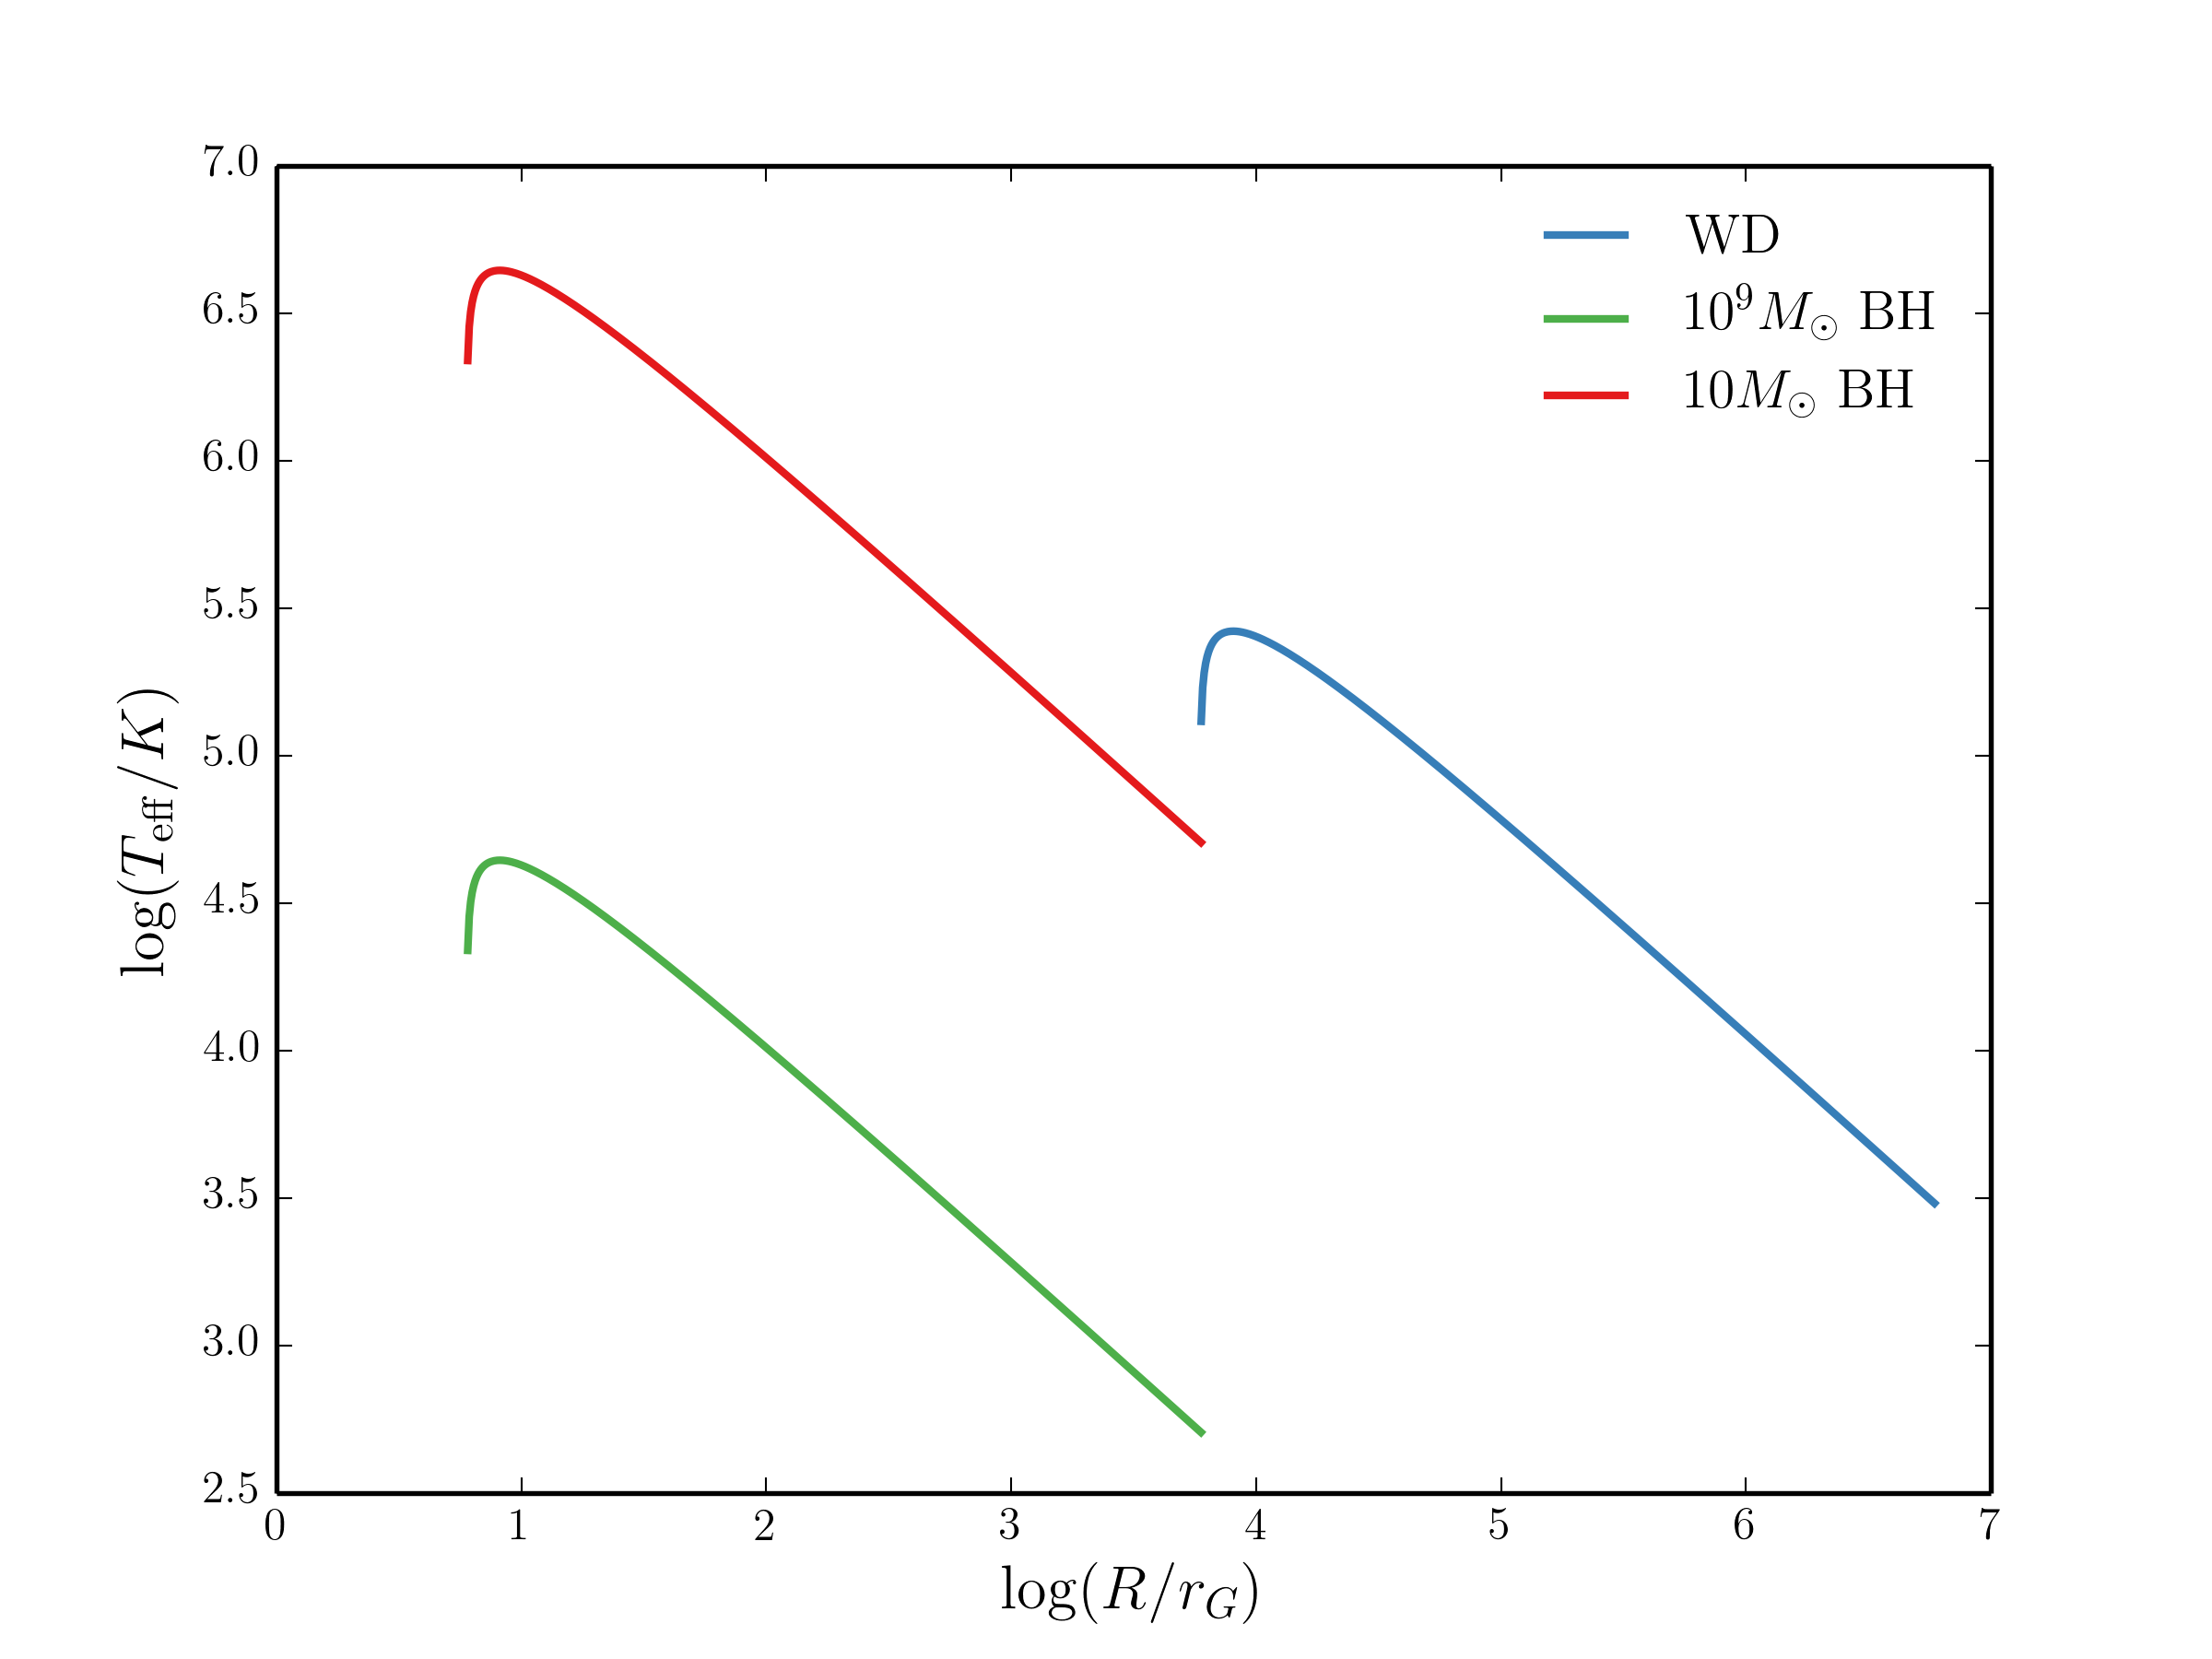
\includegraphics[width=1.0\textwidth]{figures/01-intro/disk_t.png}
\caption
[The temperature profile of an accretion disc for three different classes
of compact object.]
{
The temperature profile of an accretion disc for three different classes
of compact object.
} 
\label{fig:disk_t}
\end{figure}

\subsection{Boundary layers, black hole spin and the ISCO}

In equation~\ref{eq:ldisc} I showed that $L_{disc} = 1/2~L_{acc}$. 
One might then ask: where does the rest of the luminosity go?
The answer is dependent on the compact object in question. 
In an accreting WD, the rotating matter must eventually deposit itself 
on the surface of the WD. This is illustrated in figure~\ref{fig:omega},
which shows the angular velocity as a function of radius in a disc around
a compact object rotating with angular velocity $\Omega_*$. The boundary layer (BL)
is the region to the left of the dotted line, inside the maximum of $\Omega_K$, the Keplerian
angular velocity. The luminosity of the boundary layer is \citep{fkrbook}
\begin{equation}
L_{BL} = \frac{1}{2}\frac{GM \dot{M}}{R} \left[1 - \left(\frac{\Omega_*}{\Omega_K(R_*)}\right)\right]^2,
\end{equation}
where $\Omega_K(R_*)$ is the Keplerian angular velocity at $R_*$, assuming the thickness
of the BL is small. When $\Omega_K(R_*) \gg {\Omega_*}$, this reduces to 
$L_{BL} = 1/2~L_{acc} = L_{disc}$

In cataclysmic variables, 
BLs can be approximated with blackbodies and their temperatures estimated
indirectly via the \cite{zanstra1929} method \cite[e.g.][]{hoare1991,hoaredrew1993}.
Hopwever, they likely exhibit a variety of atomic features \citep{suleimanov2014}.
Extreme-UV (EUV) datasets have confirmed the existence of boundary layer emission
in non-magnetic CVs \citep{mauche1996}, although these observations
are limited in number.

\begin{figure}
\centering
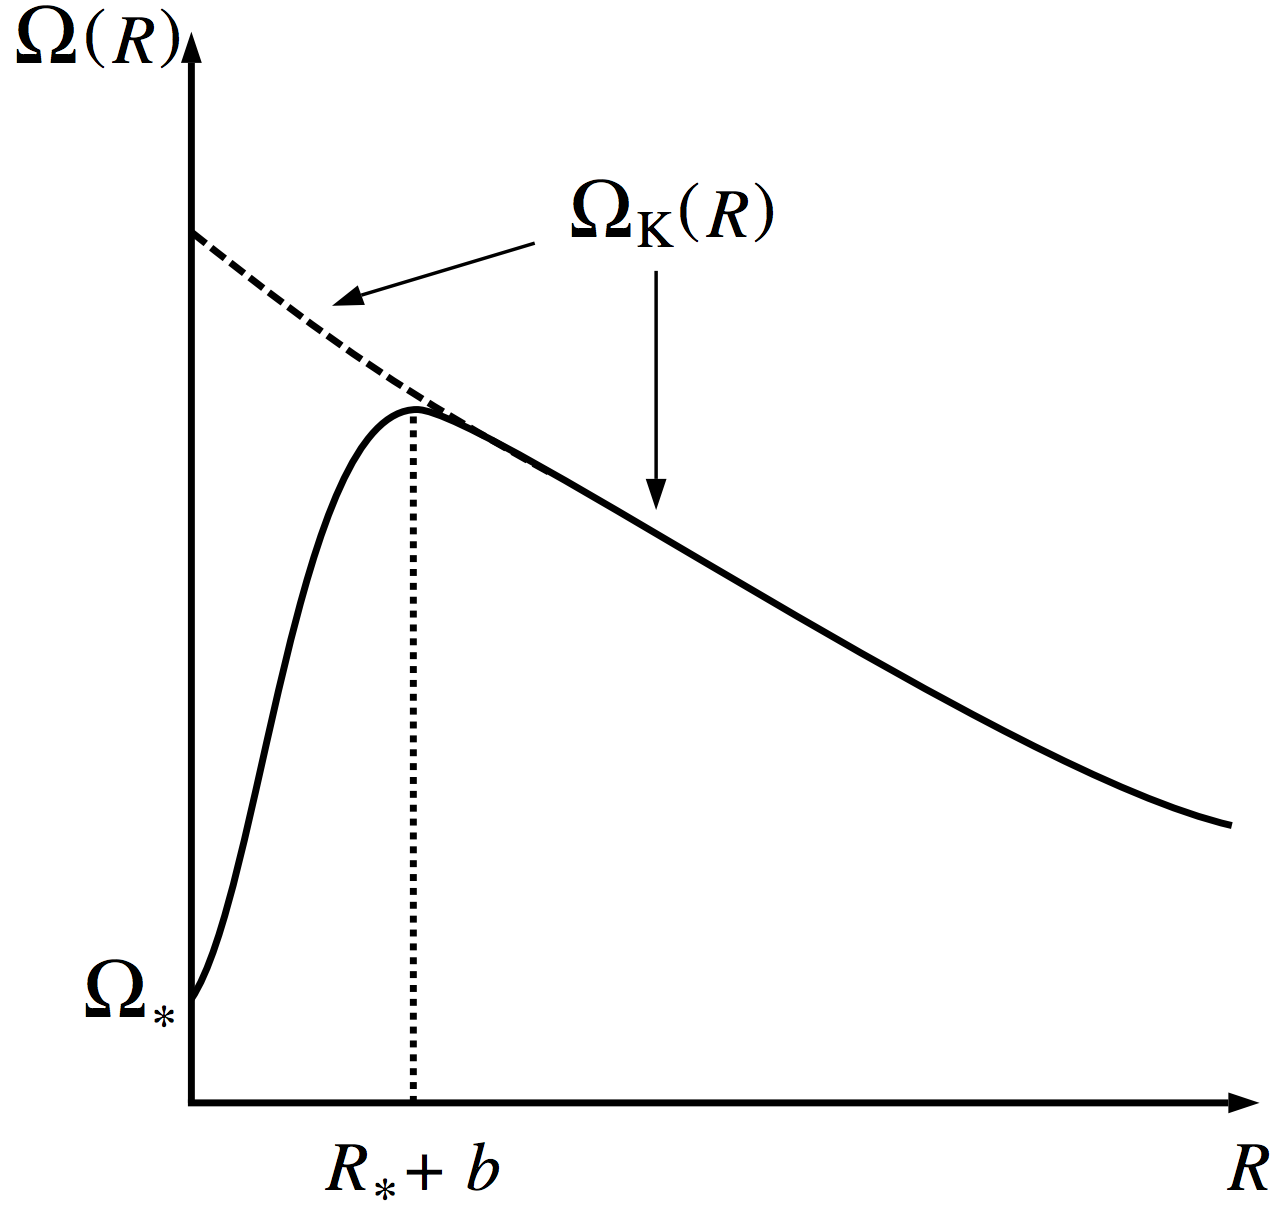
\includegraphics[width=0.7\textwidth]{figures/01-intro/omega.png}
\caption
[Angular velocity as a function of radius in an accretion disc around a rotating
compact object.]
{
{\sl Credit: Frank et al. 2002}.
Angular velocity as a function of radius in an accretion disc around a rotating
compact object with angular velocity $\Omega_*$. $\Omega_K$ is the Keplerian 
angular velocity. This graph
also helps explain why there is a turnover in the temperature-radius relation,
as $D(R)$ is proportional to the square of the {\em derivative} of this quantity.
} 
\label{fig:omega}
\end{figure}

Clearly, in BH systems a boundary layer cannot exist in the same way,
due to the lack of a physical surface. Instead, the energy must either go into
growing the BH, contributing to its angular momentum or being
channeled into a jet or other radiative source (see section~\ref{sec:disc-jet}).
The question of what happens at the inner disc edge
is complicated further by the fact that the disc cannot extend to the 
event horizon of the BH. Instead, there is an `innermost stable circular orbit' (ISCO)
beyond which the accreting matter will simply fall 
into the BH along nearly radial paths. The radius
of this orbit, $R_{ISCO}$, and the horizon radius, $R_H$,
is shown for different values of the BH spin parameter, $a_*$, 
in figure~\ref{fig:isco}, showing how matter can orbit closer to a prograde spinning BH. 
In estimating the luminosity of a Keplerian disc around a BH, 
one should really set $R_* = R_{ISCO}$ in equation~\ref{eq:eta}, giving us the interesting
result that rapidly spinning (Kerr) BHs are more radiatively efficient 
than Schwarzschild BHs.

\nocite{narayan2014, thorne1974}
\begin{figure}
\centering
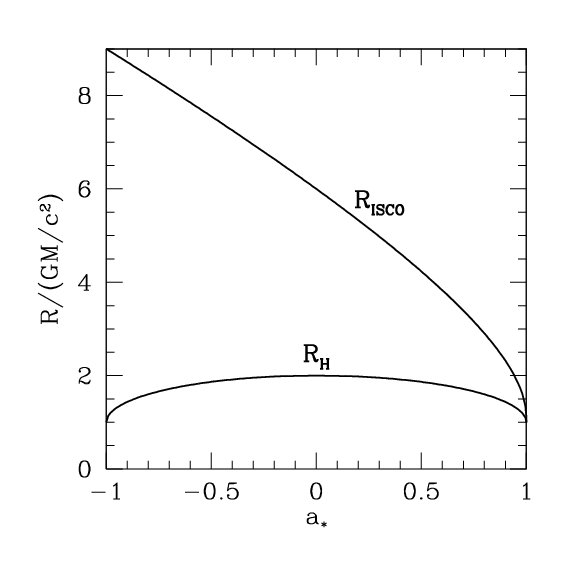
\includegraphics[width=0.7\textwidth]{figures/01-intro/isco.png}
\caption
[The radius of the ISCO, $R_{ISCO}$, and the horizon, $R_H$,
is as a function of the BH spin parameter, $a_*$.]
{
{\sl Credit: Narayan 2014.}
The radius of the ISCO, $R_{ISCO}$, and the horizon, $R_H$,
is as a function of the BH spin parameter, $a_*$. 
$a_*=0$ corresponds to a Schwarzschild BH, and $a_*=1$ and $a_*=-1$
to prograde and retrograde Kerr BHs respectively. Note that
this figure ignores the counteracting torque of photons swallowed by the BH,
which actually limits $a_*$ to a value of around $0.998$ (Thorne 1974).  
} 
\label{fig:isco}
\end{figure}


\subsection{The emergent spectrum}


\begin{figure}
\centering
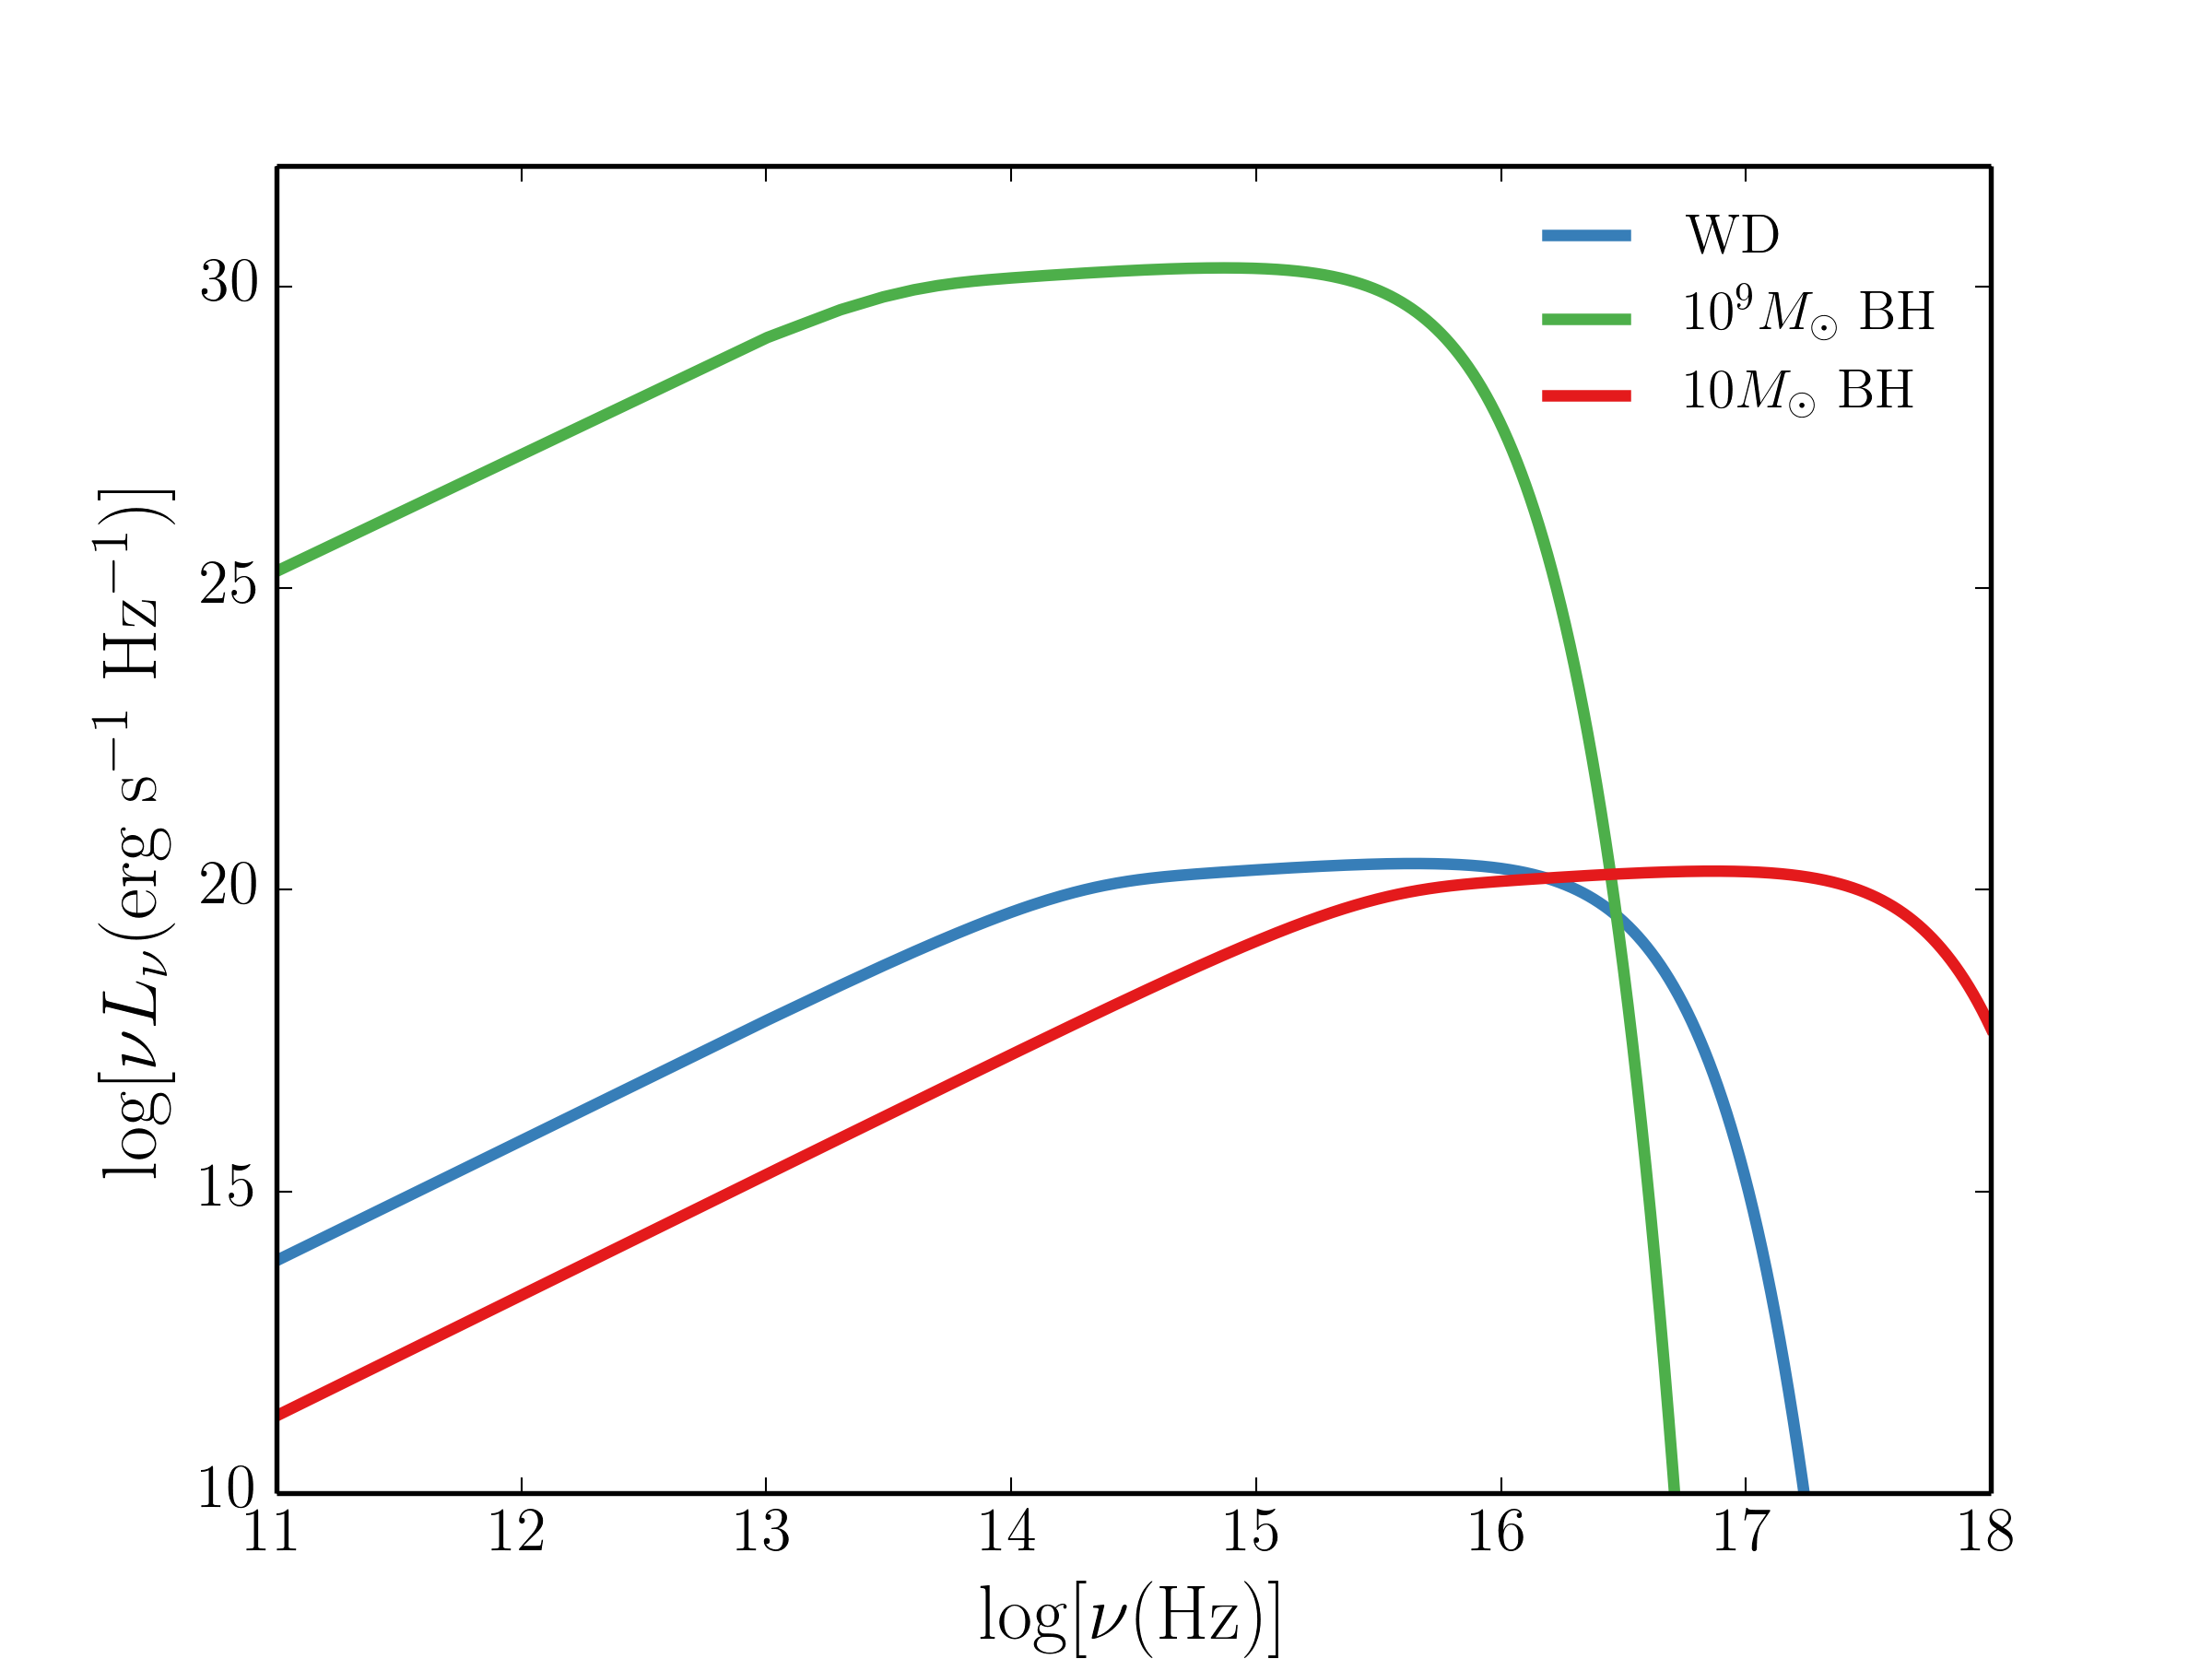
\includegraphics[width=0.8\textwidth]{figures/01-intro/disc_seds.png}
\caption
[Accretion disc SEDs for three different compact objects.]
{
Accretion disc SEDs for three different compact objects, corresponding roughly
to a quasar, an XRB and a CV. The SEDs are computed via an area-weighted sum
of blackbodies with effective temperatures governed by equation~\ref{disk_t_profile},
and the $\nu^{1/3}$ shape in the middle of the spectra can be seen.
} 
\label{fig:disc_seds}
\end{figure}

It is important to recognise that the steady-state disc treatment
{\sl does not specify the exact shape of the disc SED}. What it does do is 
say where energy is originally released. The simplest assumption is
that each annulus emits as a blackbody with temperature 
$T_{eff} (R)$, and the specific intensity through the emitting surface
thus follows the Planck Law:
\begin{equation}
B_\nu (T) = \frac{2 h \nu^3}{c^2} \frac{1}{\exp(h\nu / kT) - 1}
\label{eq:planck}
\end{equation}
Under this assumption it is possible to show that at intermediate frequencies, 
where $kT(R_{max}) \ll h \nu \ll kT_*$,
then the spectrum appears as a `stretched blackbody' with the form 
\begin{equation}
F_{\nu} \propto \nu^{1/3}.
\end{equation}
Figure~\ref{fig:disc_seds} shows the blackbody SEDs expected for the same 
objects as figure~\ref{fig:disk_t}, in
which the $\nu^{1/3}$ portion can be clearly seen.
A disc atmosphere model with frequency-dependent opacity creates a somewhat 
different (and more realistic) spectrum. 
Figure~\ref{fig:bb_v_sa} shows a comparison between a stellar atmosphere model and
blackbody model for $T_{eff}=50,000$K, showing how an annulus at that temperature
can have a significantly different spectral shape when one includes frequency-dependent opacities
in the atmosphere. It is of course possible that {\em neither} blackbody or disc atmosphere
treatments are realistic. I shall therefore devote a little time to discussing
the observational arguments for accretion discs and reviewing
the different classes of accreting objects.

\begin{figure}
\centering
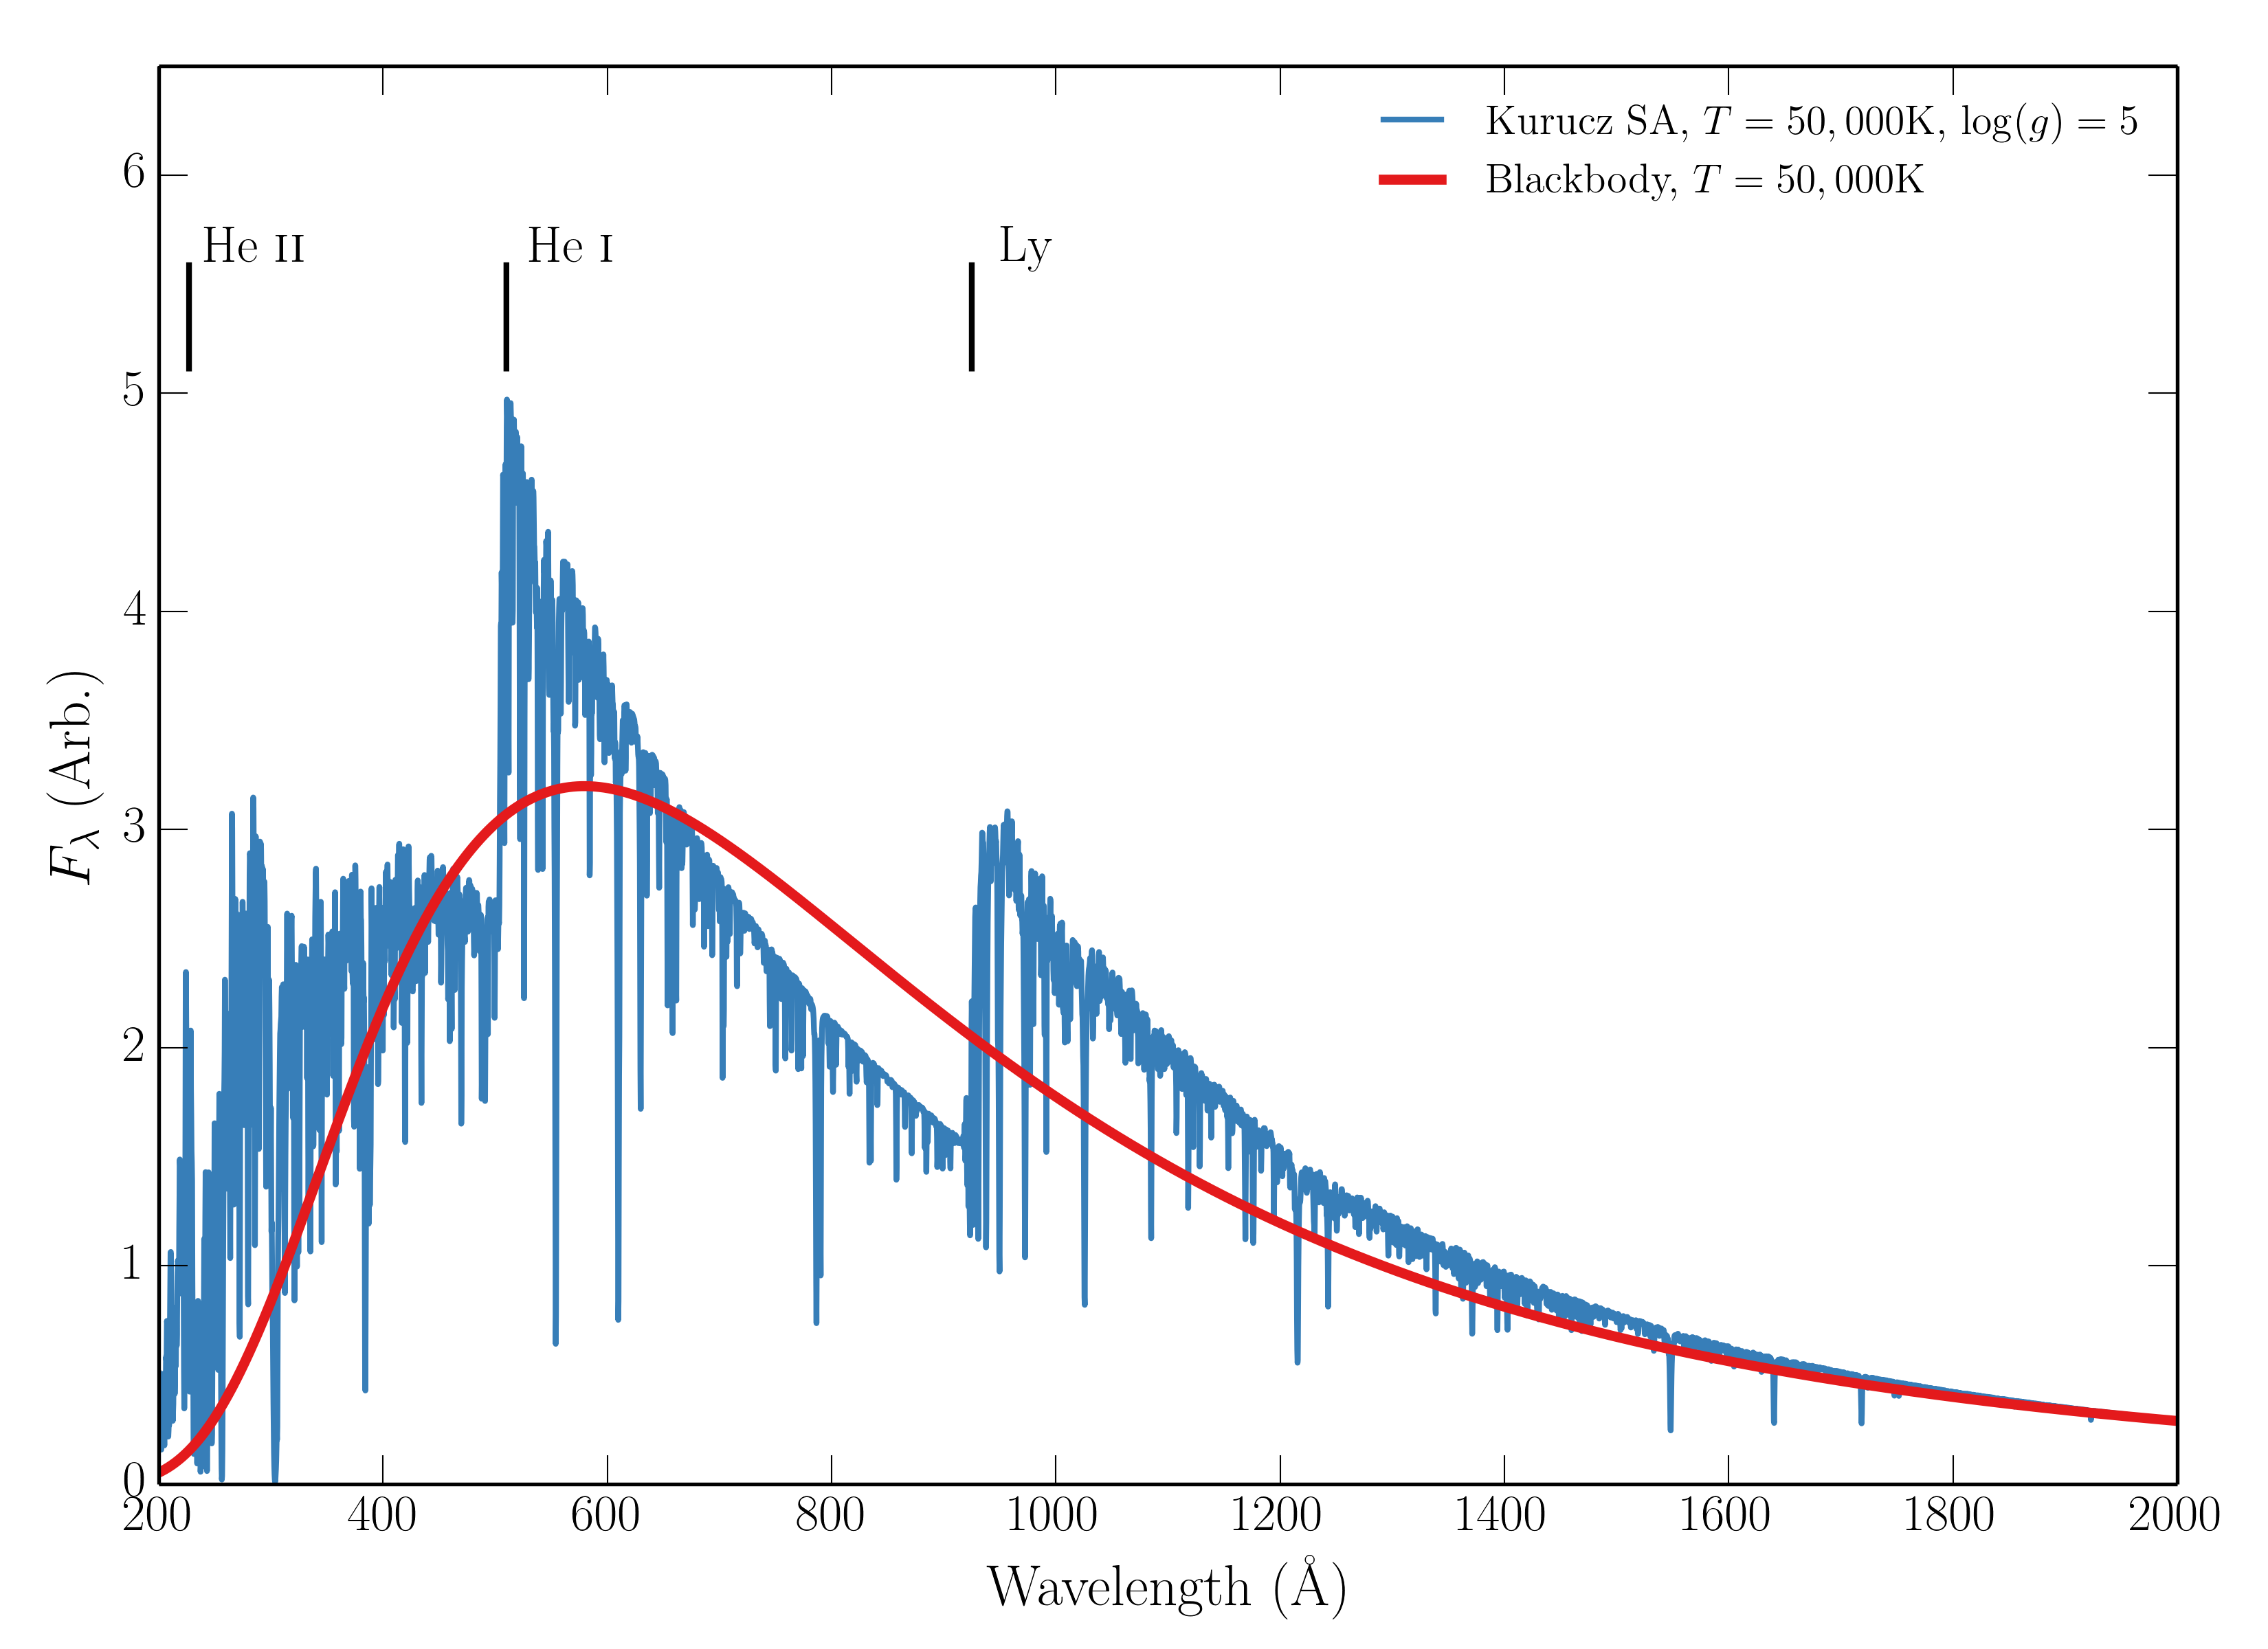
\includegraphics[width=0.8\textwidth]{figures/01-intro/bb_v_sa.png}
\caption
[A comparison between a Planck curve and Kurucz (1991) stellar atmosphere model.]
{
A comparison between a Planck curve and Kurucz (1991) stellar atmosphere model
at $T_{eff}=50,000$K and surface gravity of $\log(g)=5$. The major photoabsorption
edges are marked. Flux is reprocessed into different wavelengths by bound-free opacities,
and line blanketing also has a big effect on the spectrum. The Hydrogen and Helium lines
also experience significant pressure broadening.
} 
\label{fig:bb_v_sa}
\end{figure}


\section{Accreting Compact Binaries}

\begin{figure}
\centering
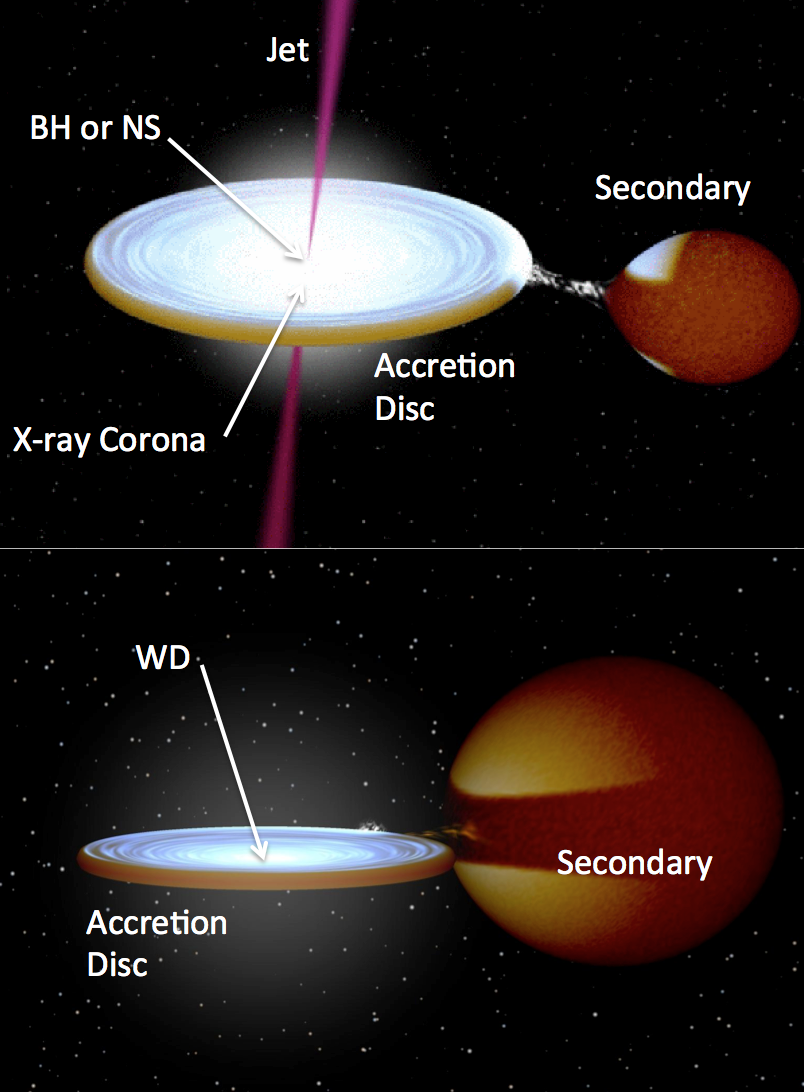
\includegraphics[width=1.0\textwidth]{figures/01-intro/cv_and_xrb.png}
\caption
[Artists impression of an LMXB and CV.]
{
{\sl Credit: Rob Hynes.} 
Artists impression of a low-mass X-ray binary (top) and
cataclysmic variable (bottom). The key components are marked,
and the clear similarity in overal structure is apparent.
} 
\label{fig:cv_and_xrb}
\end{figure}

Accreting compact binaries form many different classes, 
but are all characterised by matter streaming from a donor
onto a compact object. When the compact object is more massive 
than the donor then it is designated as the `primary', 
and the companion as the `secondary'. 
In high-mass X-ray binaries (HMXBs), the opposite is formally true.
There are only two ways by which matter can transfer 
from the secondary to the compact object. One is by Roche Lobe-overflow (RLOF),
whereby stellar evolution causes the donor star to fill its Roche Lobe, the surface
of equipotential around the star. The alternative is that the donor may expel
material via a disc or radiatively driven stellar wind, 
allowing some of it to flow onto the compact object. 
Although accretion from a wind or circumstellar disc is common in 
HMXBs \citep{bartlett2013}, here I will focus on 
RLOF as it is more common in the systems that possess high-state accretion discs
and associated outflows. Two examples of these are shown in figure~\ref{fig:cv_and_xrb}


\subsection{Roche Lobe-Overflow}

Let us consider a binary system, with masses $M_1$ and $M_2$, at positions
$\vec{r}_1$ and $\vec{r}_2$. The Roche potential, $\Phi_R$, in this system 
is then
\begin{equation}
\Phi_R = - \frac{GM_1}{| \vec{r} - \vec{r}_1 |} - 
\frac{GM_2}{| \vec{r} - \vec{r}_2 |} - 1/2 (\vec{\omega} \times
 \vec{r})^2,
\label{eq:roche}
\end{equation} 
where $\vec{\omega}$ is the angular velocity of the binary and is a vector normal to
the orbital plane. This potential is plotted in figure~\ref{fig:roche} for a mass ratio, 
$q = M_2 / M_1$ of 0.25.

\begin{figure}
\centering
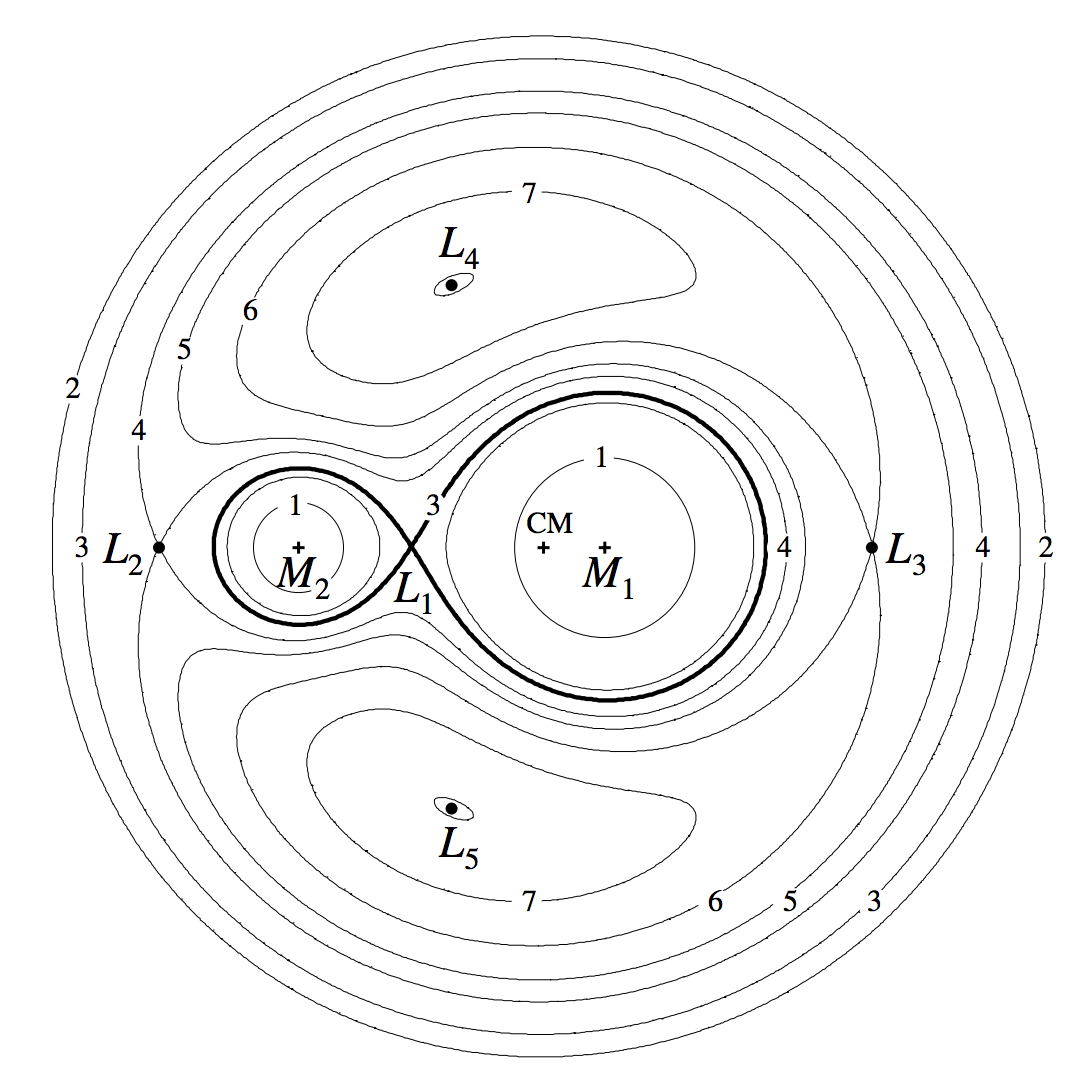
\includegraphics[width=0.7\textwidth]{figures/01-intro/roche_potential.png}
\caption
[The Roche potential in a binary system]
{
{\sl Credit: Frank et al. 2002.} 
The Roche potential in a binary system for $q = M_2 / M_1$ of 0.25.
The Lagrangian points are marked, as are the locations of the individual
and system centres of mass.
} 
\label{fig:roche}
\end{figure}

In the context of semi-detached binary systems, the most important region of the 
potential is the dumbbell shaped region enclosing the masses. Each of these
enclosed regions is known as the `Roche lobe' of the object and can be expressed 
approximately in terms of the mass ratio and separation of the system. A good approximation
for the size of the Roche lobe takes the form \citep{eggleton1983}
\begin{equation}
\frac{R_2}{a} = \frac{0.49 q^{2/3}}{0.6q^{2/3} + \ln(1+q^{1/3})}.
\label{eq:roche2}
\end{equation} 
Here $R_2$ is the radius of a sphere with the same volume as the Roche lobe for the
secondary star, which we can see depends only on $q$ and the orbital separation, 
$a$. If this secondary expands enough to fill its Roche lobe, then matter
will fall onto the other object. This process is known as Roche Lobe overflow (RLOF),
and is vitally important in astrophysics. Although caused by stellar evolution,
any accretion from RLOF will affect the mass ratio of the binary system 
and thus itself affects the evolution
of binary systems. This helps determine the orbital period
distribution of binaries \citep[e.g.][]{knigge2011_evo} 
as well as affecting the delay time distribution
of Type Ia Supernovae, for which CVs are one of the progenitor candidates 
\citep[e.g.][]{wang2012}.
It is also worth noting that the existence of gravitational waves has been 
required in models to explain the orbital period evolution of CVs since
the 1960s \citep{kraft1962}. 


\subsection{Cataclysmic Variables}

Cataclysmic variables (CVs) are systems in which a WD
accretes matter from a donor star via Roche-lobe overflow 
\citep[see the `CV bible', ][]{warnerbook}. 
CVs are not always dominated by their accretion luminosity; 
classical novae and super soft sources 
(SSS) emit mostly due to nuclear burning or detonation on the WD surface.
Accretion dominated CVs -- the focus here -- can be classified according to the 
magnetic field strength of the WD ($B_{WD} $) and photometric activity. 
Magnetic systems are classified as either `Polars' ($B_{WD} \gtrsim 10^7$~G)
or `Intermediate Polars' ($10^6 \lesssim B_{WD}  \gtrsim 10^7$~G);
in these systems the accretion flow inside the some critical radius 
(related to the Alfven radius)
is dominated by the WDs magnetic field \citep[e.g.][]{patterson1994}. 
In polars, this radius is large enough, due to the strong magnetic field,
that no disc forms at all \citep{liebert1985}.
When $B_{WD}  \lesssim 10^6$~G then the accreting material can fall
onto the WD via a disc, and the CV is classified as non-magnetic.
There are two main types of non-magnetic CVs; dwarf novae and nova-like
variables.

\subsubsection{Dwarf Novae and the Disc-instability Model}

Dwarf novae (DNe) are CVs that are characterised 
by repeated periods of quiescence and dramatic outburst. One of the 
most famous DNe is SS Cyg, whose light curve is shown in 
figure~\ref{fig:sscyg}. The repeated outbursts can be clearly seen, and
SS Cyg itself has been undergoing this behaviour for the full century 
for which it has been observed. A spectrum over the course of a 
typical outburst is shown in figure~\ref{fig:sscyg_spec}, 
and is characterised by the appearance of an optically thick
accretion disc continuum -- note the similarity to the 
stellar atmosphere disc spectrum computed in section~\ref{sec:alpha_disc},
and to the intermediate inclination nova-like variables discussed in the next
section.

The leading scnario for explaining DN outbursts, and in fact also the outbursts
in low mass X-ray binaries or `soft X-ray transients',
is the disc-instability model 
\citep[DIM; ][]{osaki1974,lasota2001}. 
In this model, a gradual increase in supply rate from the donor star 
(and hence surface density in the disc) 
causes the disc to heat up. Eventually, the disc hits a critical temperature,
around $7000$~K, and becomes ionized. Now the surface density in the disc
can increase significantly, and the disc becomes geometrically thin and
optically thick. Most importantly, it can undergo efficient radiative
cooling, and a significant increase in brightness is observed.

\begin{figure}
\centering
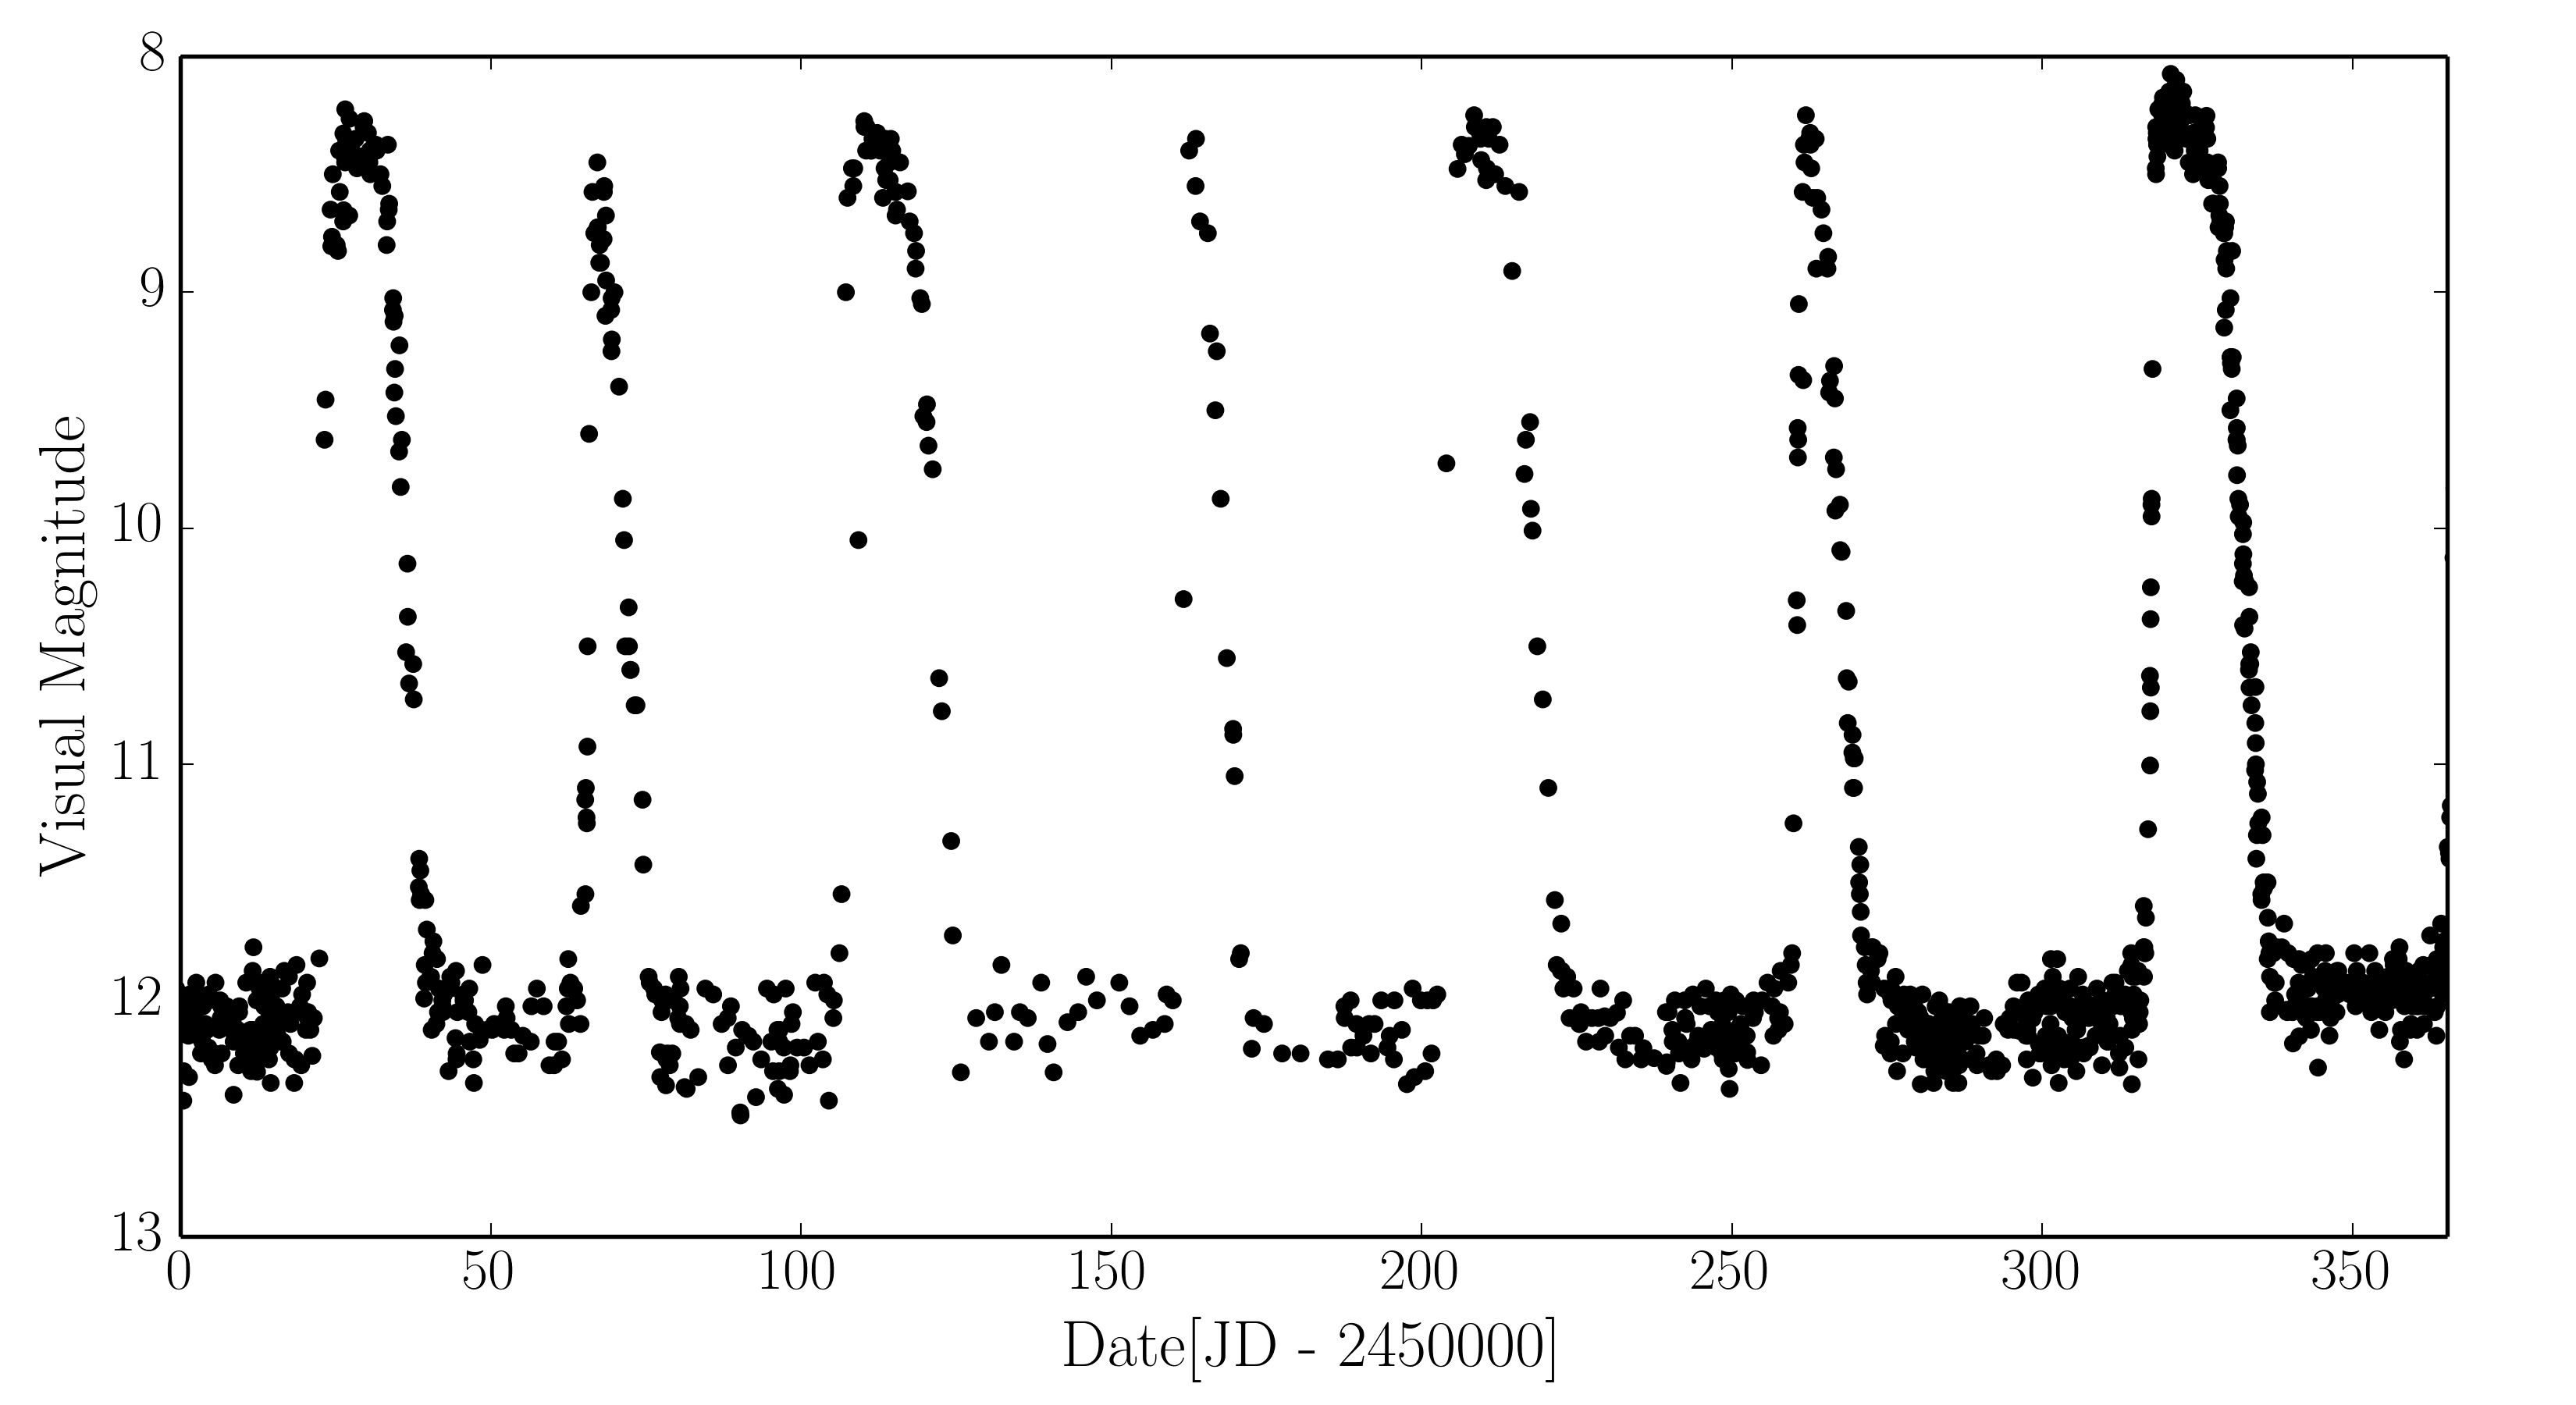
\includegraphics[width=1.0\textwidth]{figures/01-intro/lc_sscyg.png}
\caption
[A year in the life of SS Cyg.]
{
{\sl Data: AAVSO.} 
A year in the life of SS Cyg, showing the characteristic repeated
outbursts and periods of quiescence typical of a DN. SS Cyg has been
undergoing this activity since it was first observed in 1896.
} 
\label{fig:sscyg}
\end{figure}

\nocite{dhillon1996,hessman1984}
\begin{figure}
\centering
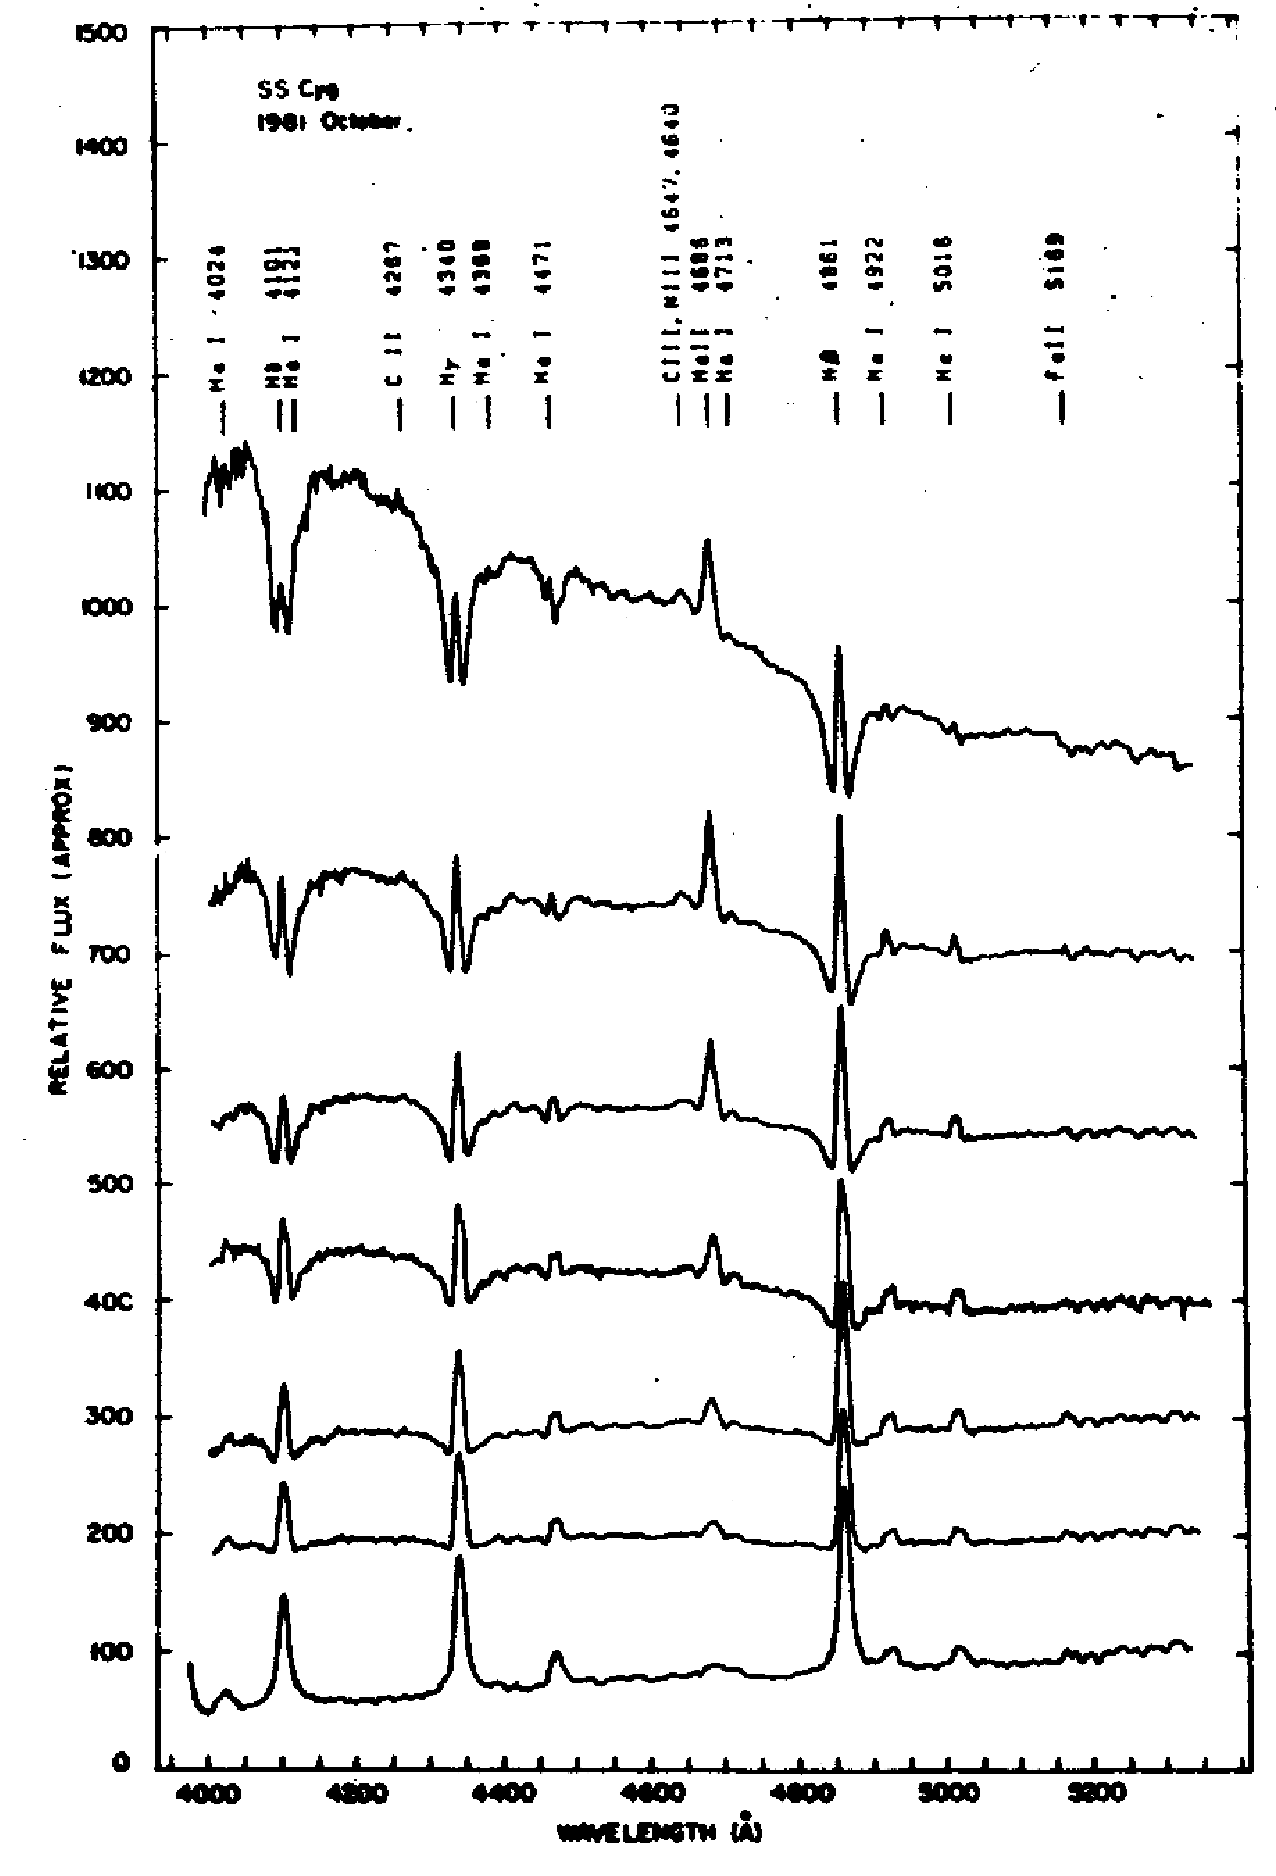
\includegraphics[width=1.0\textwidth]{figures/01-intro/sscyg_spec.png}
\caption
[Spectra of SS Cyg during an outburst cycle]
{
{\sl Credit: Hessman et al. 1984 / Dhillon et al. 1996.} 
Spectra of SS Cyg during an outburst cycle, showing the evolution from 
minimum to maximum light. The rise is characterised by the appearance of an
optically thick accretion disc spectrum. The flux scale is approximate.
} 
\label{fig:sscyg_spec}
\end{figure}

\subsubsection{Nova-like Variables}

\nocite{dhillon1996,hessman1984}
\begin{figure}
\centering
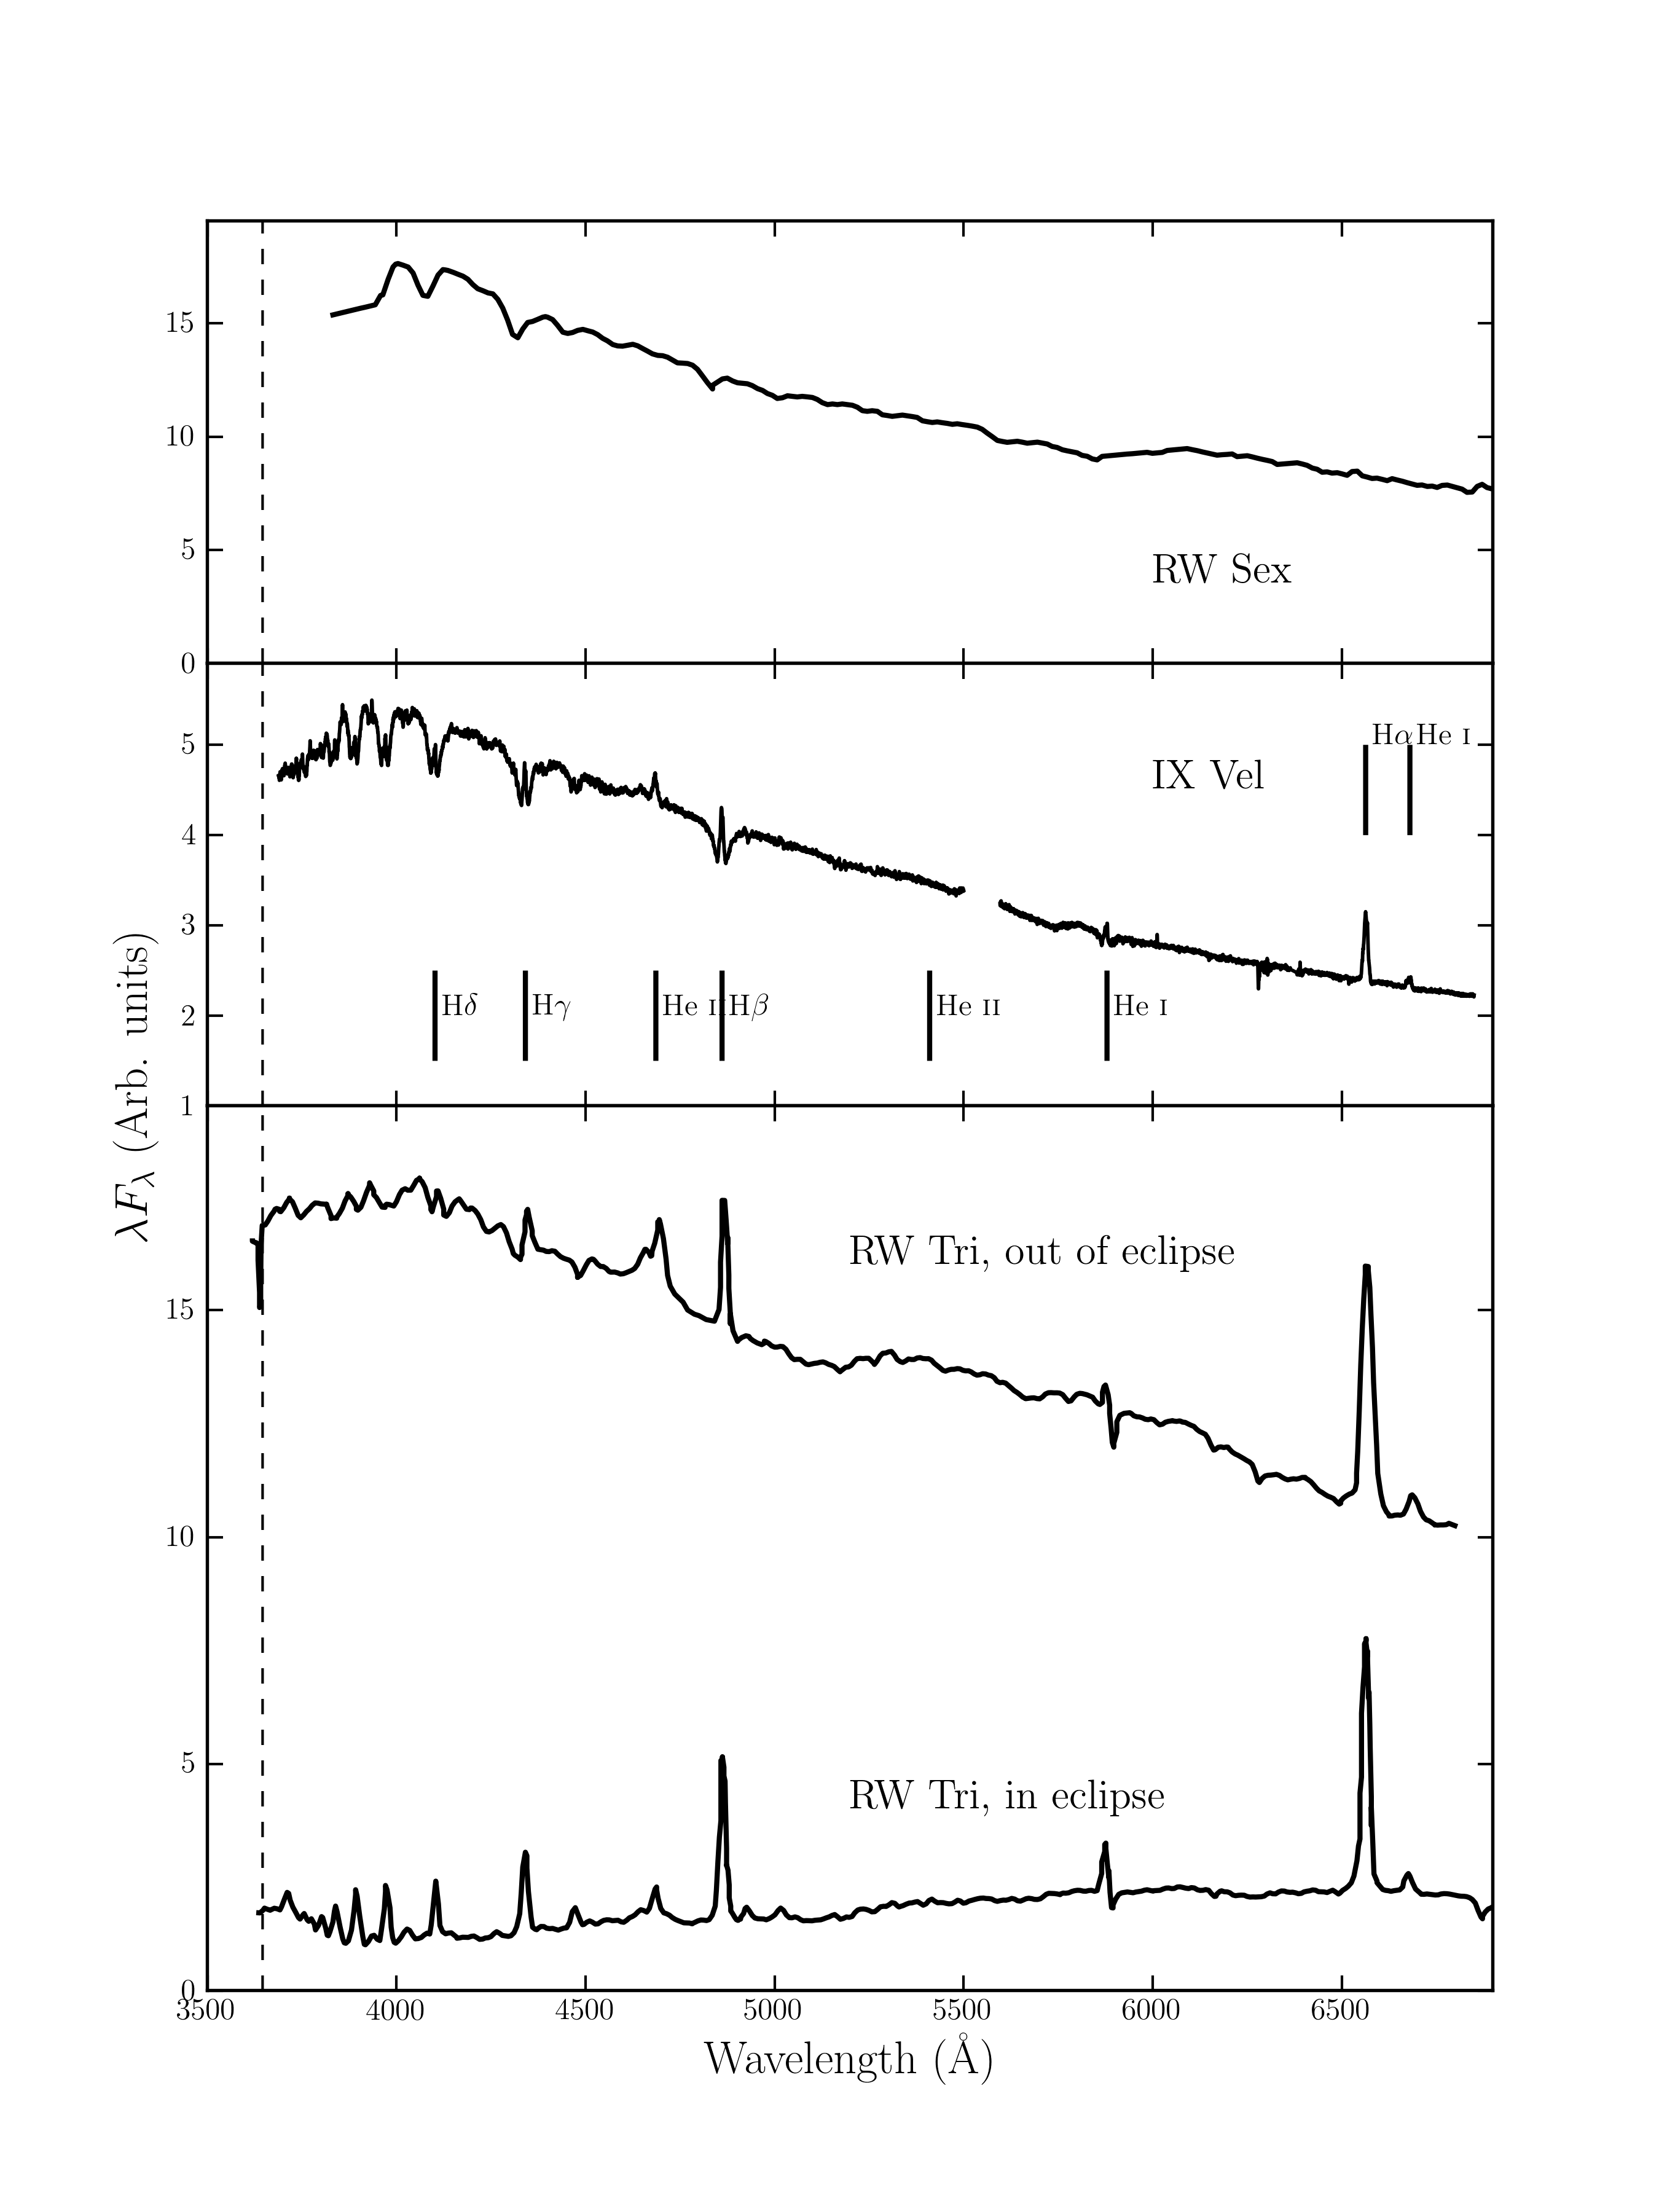
\includegraphics[width=1.0\textwidth, clip=true, trim= 0 0.6in 0 0.8in]{figures/01-intro/novalikes.png}
\caption
[Optical spectra of three nova-like variables.]
{
Optical spectra of three nova-like variables: 
RW Sex (top; Beuermann et al. 1992),
IX Vel (top middle; A. F. Pala \& B. T. Gaensicke, private communication) 
and RW Tri in and out of eclipse (bottom two panels; Groot et al. 2004).
The data for RW Sex and RW Tri were digitized from the respective publications,
and the IX Vel spectrum was obtained using the XSHOOTER spectrograph 
on the Very Large Telescope on 2014 October 10.
These systems have approximate inclinations of 
$30^\circ$, $60^\circ$ and $80^\circ$ respectively. 
The trend of increasing Balmer line emission with inclination can be seen.
In RW Tri strong single-peaked emission in the Balmer lines is seen even
in eclipse, indicating that the lines may be formed in a spatially
extensive disc wind, and there is even a suggestion 
of a (potentially wind-formed) recombination continuum in the eclipsed
spectrum. I have attempted to show each spectrum over a similar dynamic range.
} 
\label{fig:NL_spec}
\end{figure}

Nova-like variables (NLs) are similar to DNe,
except that the disc is always in a relatively 
high-accretion-rate state ($\dot{M} \sim 10^{-8}$~M$_{\odot}$~yr$^{-1}$).
NLs are therefore one of the best `laboratories' for testing the steady-state
accretion disc theory described in section~\ref{sec:alpha_disc}.
In the optical, NLs generally exhibit a series of H and He emission 
lines superposed on a blue continuum. In many
cases, and particularly in the SW~Sex subclass of NLs
\citep{HSK86,DR95}, these lines are single-peaked. This is contrary to
theoretical expectations for lines formed in accretion discs, which
are predicted to be double-peaked \citep{smak1981, hornemarsh1986}. 
{\em Low-state} CVs (dwarf novae in quiescence) do, in fact,
exhibit such double-peaked lines \citep{marshhorne1990}. 

\nocite{dhillon1996,hessman1984}
\begin{figure}
\centering
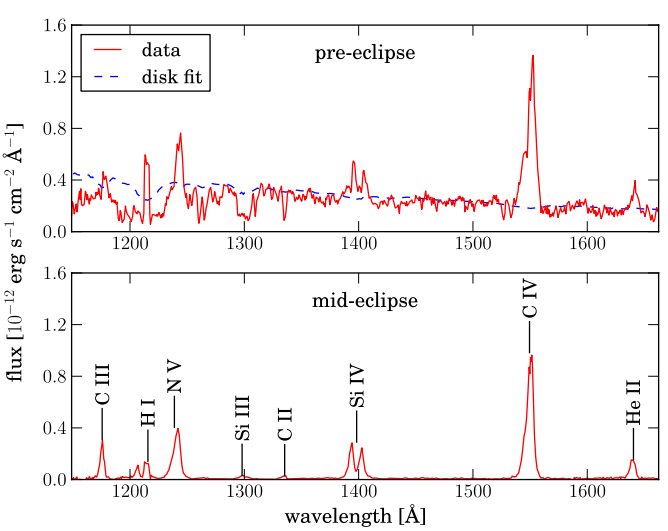
\includegraphics[width=1.0\textwidth]{figures/02-outflows/rwtri_noe.png}
\caption
[UV spectrum of RW Tri in and out of eclipse.]
{
{\sl Credit: Noebauer et al. 2010}.
UV spectrum of RW Tri in and out of eclipse, showing strong lines in 
\civfull\ and \la, among others.
} 
\label{fig:NL_spec}
\end{figure}


The UV spectra of NLs also show strong emission lines, and at 
low to intermediate inclinations dramatic blue-shifted absorption lines
can be seen in some objects. The emission line equivalent widths
in both the optical and the UV show clear correlations with 
inclination \citep{hessman1984,echevarria1988,noebauer}. 
This can be seen clearly in figure~\ref{fig:NL_spec}, and is connected to
the correlation between line strength and absolute magnitude found by \cite{patterson1984};
that is, the decrease in equivalent width at low inclination is caused by an {\em increase}
in continuum flux. This is discussed further in chapters 4 and 6, but also has 
relevance to AGN and quasar unification schemes mentioned later in this introduction.
The optical and UV spectra of NL CVs are discussed further
in the context of winds in chapter 2.

\subsection{Low Mass X-ray Binaries}

Low-mass X-ray binaries (LMXBs) 
are similar to CVs in structure (see figure~\ref{fig:cv_and_xrb}), 
but the compact object
is either a neutron star (NS) or black hole (BH). The accretion disc 
emits in the soft X-ray regime, and an additional hard X-ray power law is also 
seen in the spectrum. This hard component is normally attributed
to Compton up-scattering of seed disc photons by some kind of `corona'
of hot electrons close to the BH \citep[e.g.][]{white1988,mitsuda1989,uttley2014}.
Although I do not study LMXBs directly in this thesis, it is instructive
to briefly discuss of their observational appearance as it is relevant to the links
between accretion and outflow. The discovery that XRBs and CVs follow similar 
tracks on a hardness-intensity diagram \citep{kordingDNjet2008}
is particularly interesting in this regard, especially since \cite{ponti2012}
showed that broad Fe absorption lines are only seen in the soft-state 
high-inclination systems (see section~\ref{sec:xrb_winds}). 
This implies that equatorial outflows are intrinsic to 
the accretion process. Although the driving mechanism
is probably different to CVs \citep[e.g.][]{diaztrigo2015}, 
the similarity in general structure to models for CVs and quasars is striking.


% \begin{figure}
% \centering
% 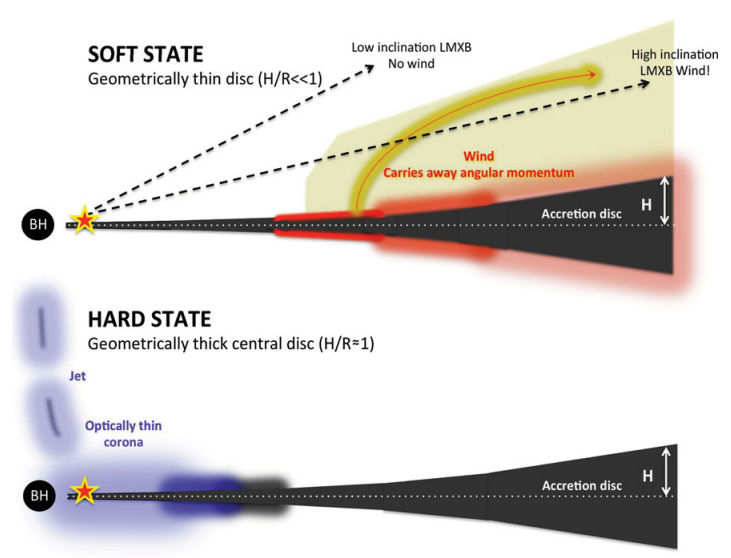
\includegraphics[width=0.7\textwidth]{figures/01-intro/ponti_wind_cartoon.png}
% \caption
% [Hardness intensity diagram for a WD, NS and BH system]
% {
% {\sl Credit: Ponti et al. 2012}
% Hardness intensity diagram for a WD, NS and BH system
% } 
% \label{fig:ponti_cartoon}
% \end{figure}


\section{Quasars and Active Galactic Nuclei}

Spectra of AGN have now been studied for over 100 years, and we have known 
that they exhibit strong, broad emission lines since the first spectrum was taken by
\cite{fath1909}. However, it wasn't until the work of \cite{seyfert1943} that the systematic 
classification of AGN really began, leading to the phrase `Seyfert galaxy'.
This label was applied to galaxies possessing a bright nucleus, spectroscopically
characterised by a blue continuum and a series of strong emission lines.
The first real physical insight into the extraordinary nature of AGN
was provided by \cite{woltjer1959}, who noted that 
(i) the nuclei must have sizes $<100$~pc,
based on the fact that they were unresolved, and (ii) the mass of the nucleus
must be very high, based on virial estimates. 
While both of these observations were based on simple arguments, the fact that these
ultra-luminous celestial objects are both {\em compact} and {\em supermassive}
is perhaps the defining insight into the nature of AGN.

Although the study of AGN was established in the optical waveband, 
radio astronomy also significantly furthered our understanding of AGN
in the mid-20th century. A number of surveys, such as the Cambridge \citep{edge1959}, 
Parkes \citep{ekers1969} and Ohio \citep{ehman1970} surveys discovered a great many 
bright radio point sources distributed isotropically across the sky.
These sources eventually became known as `quasi-stellar radio sources',
or {\em quasars}, and were soon found to be coincident with bright optical
sources or `quasi-stellar objects' (QSOs) at high 
redshifts \citep{schmidt1963,schmidt1965a,schmidt1965b}.
Nowadays, the term quasar normally has very little to do with 
radio emission and is often used interchangeably with QSO. 
Indeed, throughout this thesis I shall refer to a quasar as simply a bright, 
massive AGN; one with sufficiently high luminosity that it dominates the emission 
from its host galaxy.

One of the main classification schemes for AGN is a spectroscopic one, based on 
whether an object possesses broad emission lines in its spectrum, 
such as \civ\, broad \hb\ and
\la, in addition to the narrow lines that are always present. 
If these broad lines are seen, then the AGN is classed as type I;
if not, it is classed as type II (figure~\ref{fig:agn_templates}).
These designations were originally applied to Seyfert galaxies \citep{seyfert1943}, 
but can also be used to classify the more luminous quasar class, despite the apparent
difficulty in finding the expected number of type II sources \citep{zakamska2003}. 
This classification scheme is complicated somewhat by the existence of two
unusual types of AGN: narrow line Seyfert Is (NLSIs), which
may be explained by super-Eddington accretion \citep{done2015} 
or perhaps simply an orientation effect \citep{baldi2016},
and so-called `true type II' AGN, in which the broad line region is absent 
\citep{tran2001,shi2010} rather than obscured (see next section).
Despite this muddying of the waters, what was originally a 
clear dichotomy in spectral type provided a 
profound motivation for attempting to {\em unify} AGN via geometric arguments.


% \subsection{AGN Taxonomy}
% \label{sec:agn_taxonomy}

% In addition to Seyfert galaxies and quasars, there are a number of 
% different classes of AGN. These are broadly characterised by their spectra in the 
% optical, UV and X-ray as well as their radio behaviour. It is worth noting
% that these are observational classifications; that is, even after a century
% of study, the {\em physical} origins of the diverse behaviour of AGN
% are still an active area of research.

\begin{figure}
\centering
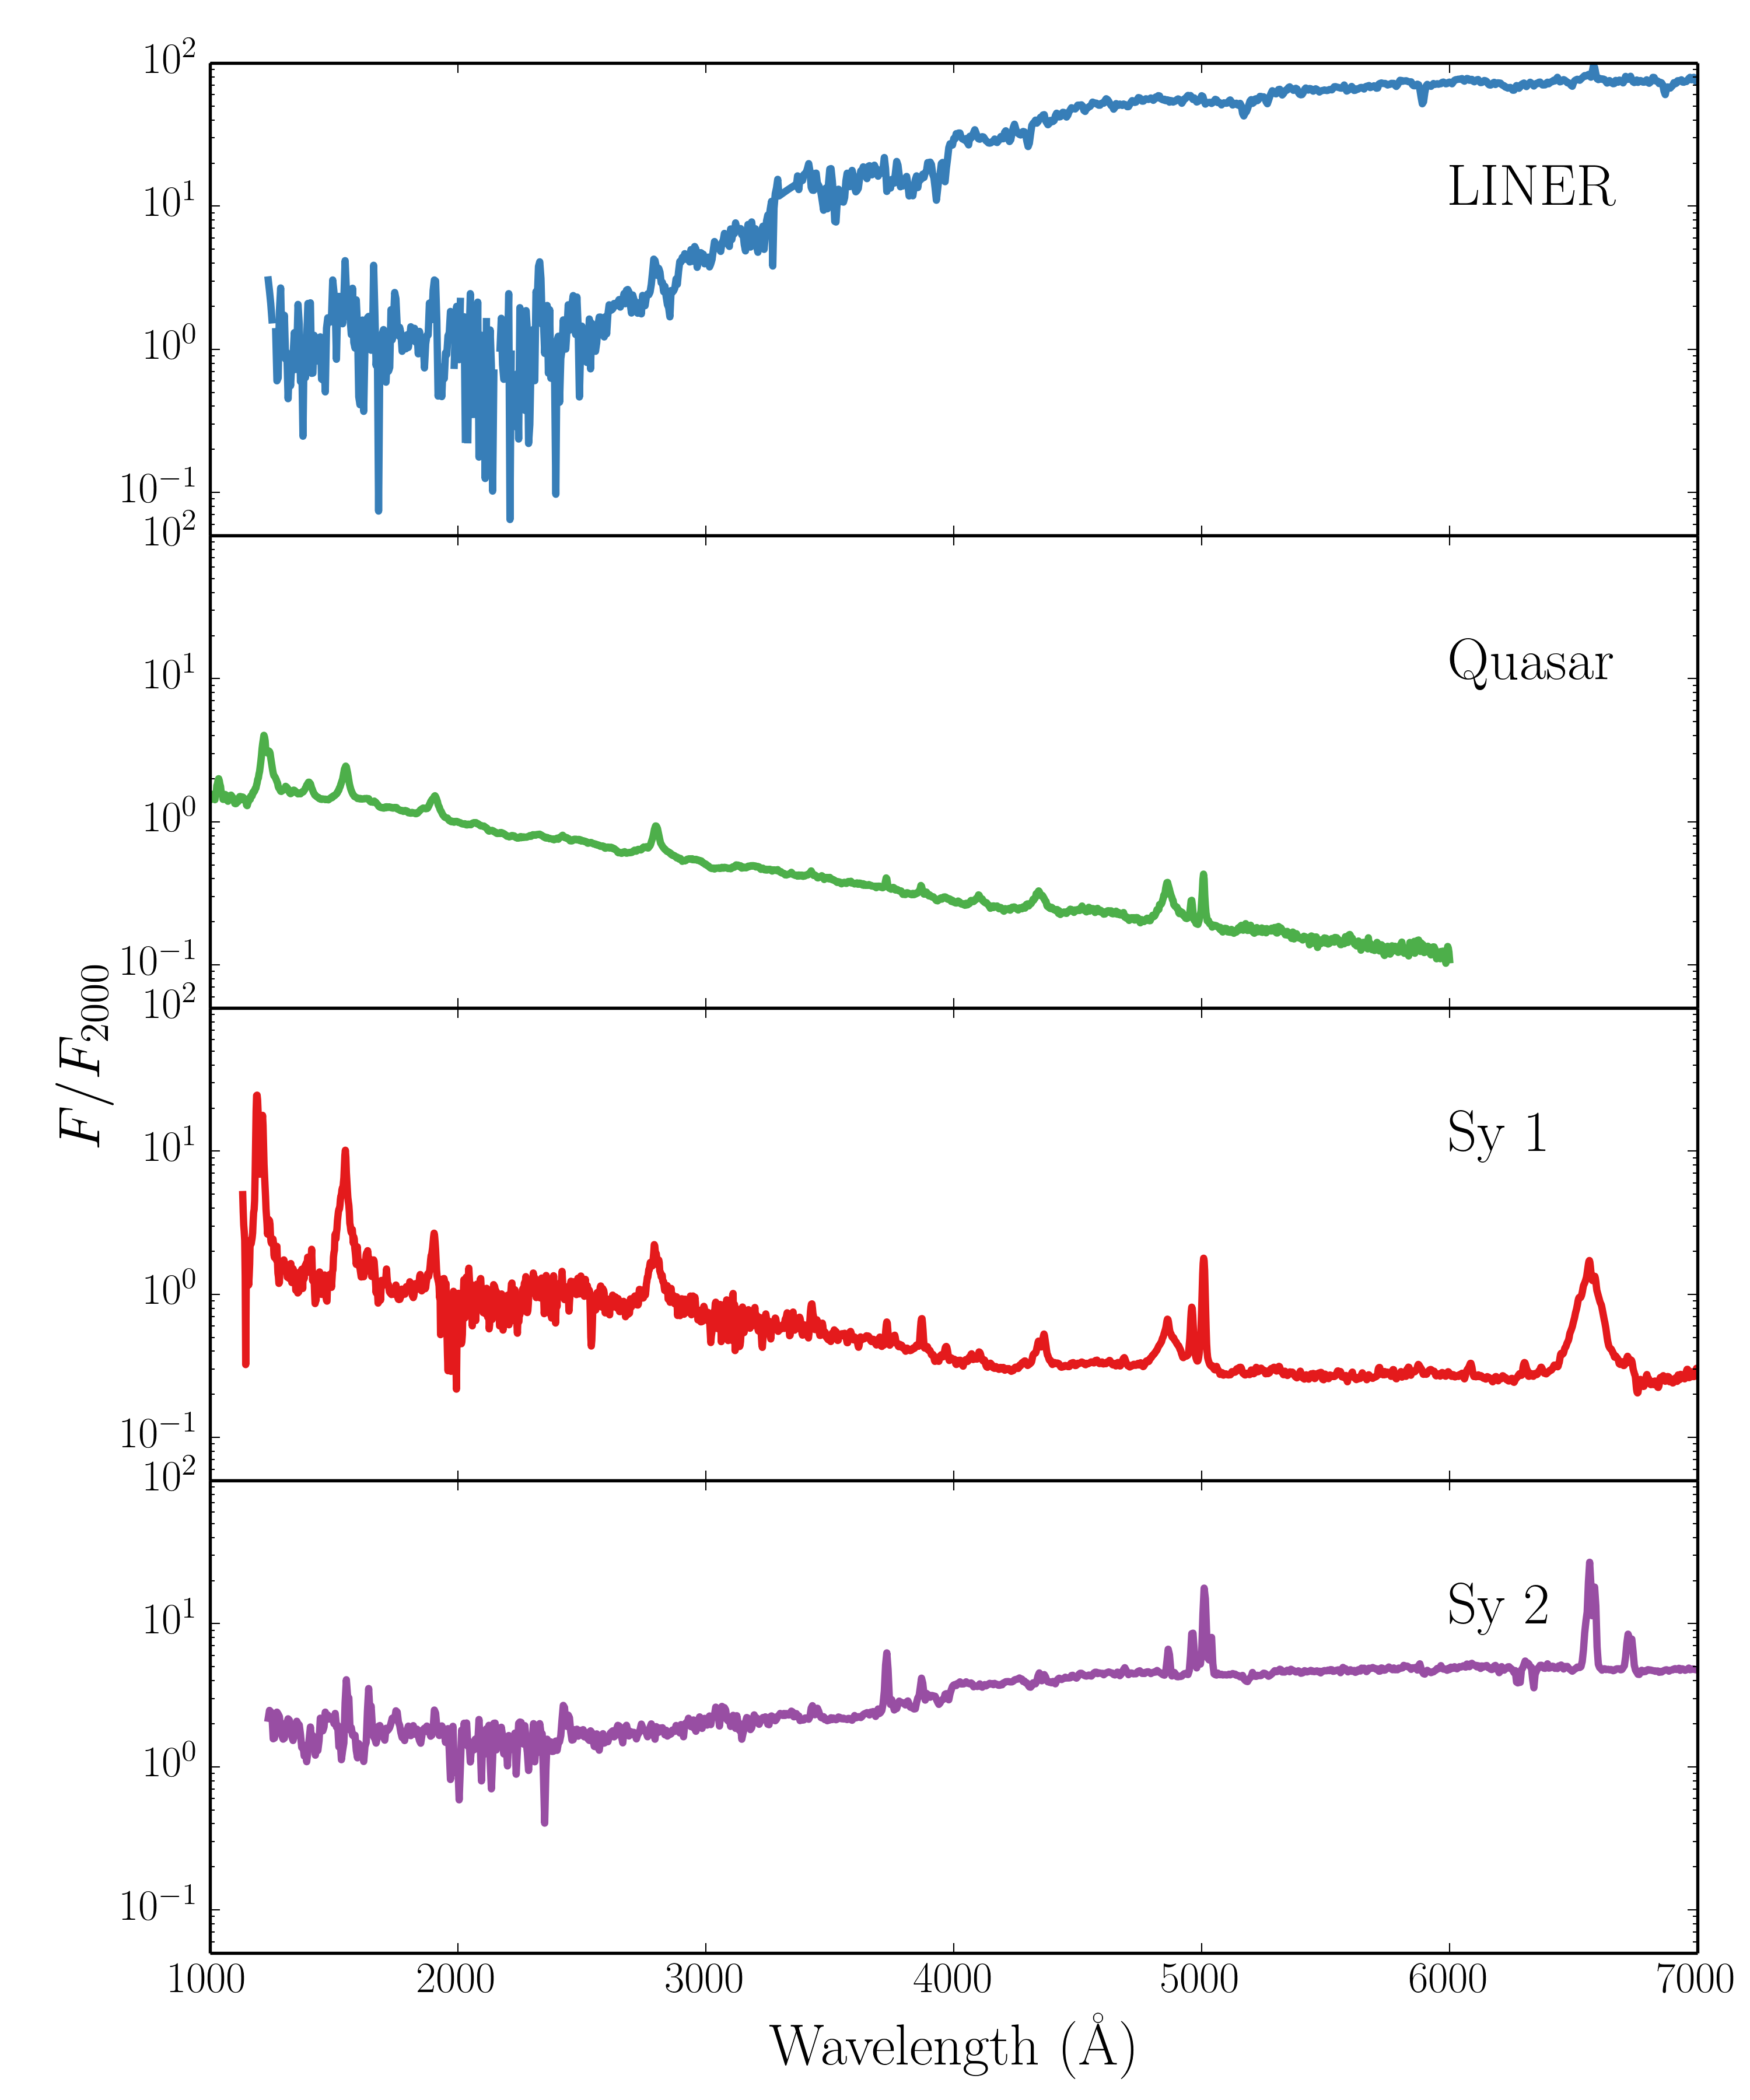
\includegraphics[width=1.0\textwidth]{figures/01-intro/agn_templates.png}
\caption
[Template spectra, from the AGN atlas, for four common types of AGN.]
{
Template spectra, from the AGN atlas, for four common types of AGN.
Obtained from \url{http://www.stsci.edu/hst/observatory/crds/cdbs_agn.html}.
} 
\label{fig:agn_templates}
\end{figure} 

% \subsubsection{Radio Galaxies}

% Radio galaxies are a broad class of AGN, of which radio-loud quasars and blazars are
% technically members, which show strong emission in the radio band. 
% The main classification scheme was proposed by \cite{FR1974}, who split
% sources according to the luminosity. FR I sources are lower in radio luminosity with a steadily decreasing surface brightness towards the edge of the radio lobes.
% FR II sources are more luminous and exhibit bright structures at the edge of their 
% radio maps. Radio galaxies are not particularly relevant here, but it is worth 
% noting that `Radio core dominance', $\log R$, is often used as an orientation indicator 
% \citep{orr1982,wills1995}. This is because more pole-on sources should, in theory, 
% be more dominated by their
% cores whereas edge-on sources should be more dominated by extended radio
% lobes. I discuss the use of orientation indicators further in chapter 6.

% \subsubsection{BL Lacs and Blazars}

% BL Lac objects -- named for the first object of the class, BL Lacertae --
% are AGN with featureless non-thermal continua 
% \citep[see figure~\ref{fig:agn_templates}, and][for a review]{falomo2014},
% in contrast to Seyfert galaxies. 
% Their optical flux is highly polarised \citep{angelstockman1980}
% and they tend to exhibit large-scale optical variability, 
% to the extent that they were originally classified as irregularly variable
% stars \citep{hoff1929}. BL Lacs are a subset of 
% a larger AGN class known as Blazars, the most luminous of which
% are known as optically violent variable (OVV) quasars \citep{wright1998}. 
% Blazars require relativistic beaming in order to explain their high 
% radio luminosities \citep{ghis1985,ghis1993}, 
% implying that the jet is orientated towards
% the observer. These objects thus have an important place in unification
% schemes (see section~\ref{agn_unification}), and
% allow us to measure bulk Lorentz factors in radio jets, which
% can be as high as $\sim50$ \citep{begelman2008}.

% \subsubsection{Obscured and Compton-thick AGN}

% \subsubsection{Low-luminosity AGN}


\subsection{AGN Unification and the dusty Torus}
\label{agn_unification}

Although Seyfert had identified type 1 and 2 AGN, a physical explanation
for this dichotomy was not forthcoming until a study by \cite[][AM85]{antonucci1985}.
They showed unambiguously that the nearby Seyfert 2 NGC~1068 is simply an obscured
type 1 AGN, by finding that broad emission lines appeared in the spectrum of
{\em polarised} flux. This provided the basis for the first successful attempt
to unify AGN behaviour, as it elegantly 
explained the apparent disconnect between the two types of 
AGN as simply a viewing angle effect; at one angle, an observer could look directly
into the broad line region (BLR) near the nucleus, but at Type 2 angles
this region was hidden from view.
The obscuring structure became known as the `torus' \citep{krolik1986}, 
due to its proposed geometry, and it was soon realised that this structure
may be made of dust, in which case it could also be responsible for the infra-red (IR)
bump in AGN \citep{neugebauer1979}.

\cite[][UP95]{UP95} went further than the original unification model
proposed by AM85, as they also tried to account for the dichotomy in 
AGN radio properties (radio-loud/radio-quiet).
The picture they proposed is shown in figure~\ref{fig:unification}.
This model attempts to explain all of the types of AGN 
% described in section~\ref{sec:agn_taxonomy} 
merely as a function of viewing angle
and presence, or absence, of a radio jet. Models such as this also 
describe the series of `bumps' observed in AGN -- the portions
of the spectrum that dominate the luminosity, shown in figure~\ref{fig:quasar_sed}. 
In most models, the `Big Blue Bump (BBB)' is ascribed to thermal 
emission from an accretion disc, and the `Small Blue Bump' to optically 
thin Balmer continuum and Fe~\textsc{ii} emission from the BLR.
The latter can just be seen between $\sim2000$\AA\ and 
$\sim4000$\AA\ in the Seyfert 1 and 
quasar templates in figure~\ref{fig:agn_templates}.
Our understanding of the BBB is still unsatisfactory 
(see section~\ref{sec:disc_continuum}).

\begin{figure}
\centering
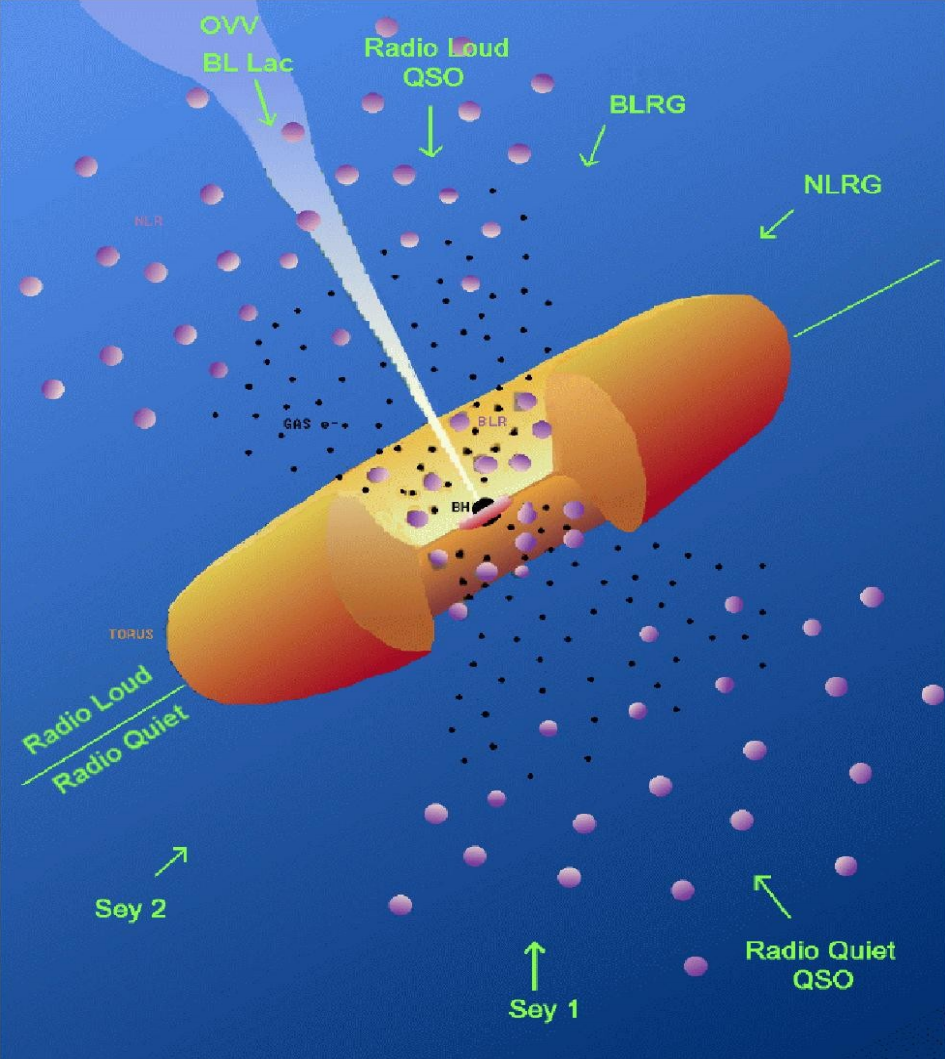
\includegraphics[width=1.0\textwidth]{figures/01-intro/up95.png}
\caption
[A unified scheme for AGN.]
{
A unified scheme for AGN.
} 
\label{fig:unification}
\end{figure} 

\nocite{elvis1994}
\begin{figure}
\centering
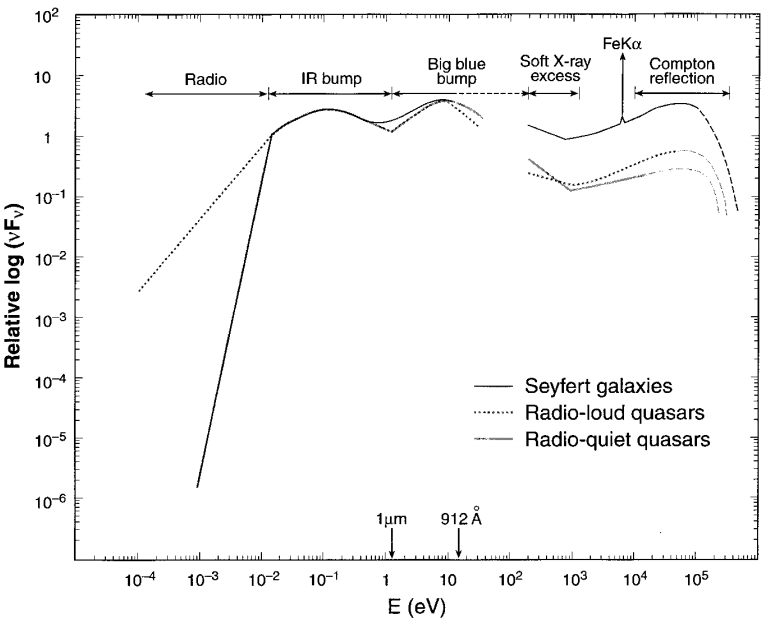
\includegraphics[width=1.0\textwidth]{figures/01-intro/agn_sed.png}
\caption
[Broadband SEDs for different AGN SEDs]
{
{\sl Credit: Koratkar \& Blaes 1999}
Approximate average broadband SEDs for a few types of AGN. The series of 
characteristic bumps can be clearly seen. 
The Soft-X-ray excess is also visible
(see section~\ref{sec:sxxs}).
} 
\label{fig:quasar_sed}
\end{figure}

Since the seminal works by AM85 and UP95, 
the picture has become somewhat more complicated. 
Variable X-ray absorption has been detected in so-called `changing look'
AGN \citep{matt2003,puccetti2007}, including even NGC 1068 itself \citep{marinucci2016}.
Changes in type have also been seen in the optical lines; 
the broad H$\beta$ component in some AGN can dramatically disappear or reappear
\citep[e.g.][]{tohline1976,cohen1986,denney2014}. 
The explanation for this could be variable absorption \citep{elitzur2012}
or a change in the accretion state of the disc. In the latter case,
it has even been suggested that a disc wind could be directly responsible
for this switch \citep{elitzur2014}.
Furthermore, dusty {\em polar} outflows
have been found to be important IR emitters \citep{hoenig2013}, implying
that, even when it comes to dust, the torus is not the whole picture.
Despite these complications, the AGN torus unification picture still
explains a lot of AGN phenomenology, and represents a useful framework 
that can be tested with observations. 


\subsection{X-ray Properties of AGN}

Approximately $10\%$ of the bolometric luminosity of AGN
comes out in the X-ray band, between $\sim0.1$ and $\sim100$~keV.
Thus, AGN dominate the cosmic X-ray background \citep{madau1994}.
The hard X-ray emission typically follows a power law shape with spectral
index -0.9 \citep[e.g.][]{koratkar1999}, 
widely considered, as in LMXBs, to come from a hot `corona' of 
electrons close to the BH that upscatters disc seed photons
\citep[e.g.][]{haardt1991}. The compactness of this X-ray corona
has been confirmed by microlensing \citep{chartas2009, dai2010} 
and variability studies \citep{green1993,crenshaw1996,risaliti2007}. 
Indeed, X-rays in AGN can be highly variable, both in terms of their intrinsic 
X-ray emission, but also due to changes in the absorption characteristics 
\citep{risaliti2002,miller2008,connolly2014}.
I discuss X-ray absorption in more detail, particularly with respect to disc winds, 
in chapter 2.

The hard X-ray spectra AGN also tend to exhibit a number of reflection features. 
Typically, these consist of a strong Fe K$\alpha$ emission line and a `Compton hump'
at high energies. The latter is produced by Compton down-scattering 
of high energy photons \citep{pounds1989,nandra1994}.
It is still unclear exactly where these features originate, 
but a common interpretation is that they are caused by 
reflection off the inner parts of the accretion disc 
\citep{fabian1995,iwasawa1996b,reynolds1999}.
If this is the case, and the broadening of the iron line is relativistic,
this would allow for measurements of the BH spin 
\citep{laor1991,iwasawa1996a,dabrowski1997}.
This hypothesis is somewhat controversial. Multiple authors have found that 
many of the relativistic features supposedly imprinted by BH spin can in fact be explained
by Comptonisation or absorption \citep[e.g.][]{misra1998,miller2013}, 
and radiative transfer modelling has shown that
an outflow can naturally produce the characteristic broad red Fe K$\alpha$ wing \citep{sim2010}.

In Compton-thick AGN, the intrinsic continuum is heavily absorbed with columns of
$N_H\sim10^{24}$~cm$^{-2}$ -- this absorption is normally attributed to the dusty torus, 
but disc winds could also contribute. Compton-thick AGN are required 
in large numbers in order to explain the cosmic X-ray background \citep{setti1989}.
In these sources, reflection features can actually dominate the X-ray spectrum 
\citep{alexander2011,gandhi2013}, but the Fe line is formed from low ionization
stages of Fe on $\sim0.1$~pc scales \citep{gandhi2015}.


\subsubsection{The Soft X-ray Excess}
\label{sec:sxxs}

If one interpolates between the $\nu^{1/3}$ law from the BBB in the UV, and the power law
in the hard X-rays, a curious excess of flux is often found
in type 1 AGN \citep[see figure~\ref{fig:quasar_sed}, and][]{koratkar1999}. 
This is known as the soft X-ray excess (SXXS), which is too 
hot to be explained by thermal disc emission, as a thin disc around an AGN should
never approach the temperatures required. Many models have been proposed to
explain this excess, including relativistically smeared 
photoabsorption \citep{gierlinskidone2004b,gierlinskidone2006}, 
relativistically smeared line and free-free emission \citep{rossfabian2005} 
and a variety of cool Comptonised component geometries such as an 
inner accretion flow \citep{magdiarz1998,done2012} 
and thin layer on top of the disc \citep{januik2001}. 
While the SXXS poses a challenge to
the simplest pictures of AGN, it may also solve some of the issues, as
some of the geometries proposed may help to explain the 
accretion disc size problem discussed in 
section~\ref{sec:disc_continuum} \citep{gardnerdone2016}.

\subsection{The Broad Line Region: Connection to winds and unification}

In the UP95 unification model, the broad emission lines
come from a series of virialised clouds close to the disc plane.
As noted by \cite[][hereafter MCGV95]{MCGV95}, there are a number of problems with
the BLR `cloud' model, perhaps most notably that there is no obvious 
physical origin for such virialised clouds. 
Testing alternative models for the BLR is therefore important.
Indeed, MCGV95 proposed a disc wind model in order to explain both BALs and BELs
in quasars. A disc wind model was also  discussed by \cite{elvis2000}, 
who proposed a structure for quasars that attempted to explain much 
of the behaviour of luminous AGN
merely as a function of viewing angle. Outflow models are discussed further in section~2.
The philosophy of these models is that, before invoking additional
degrees of freedom in a model, we should first test if known quasar phenomenology 
(disc winds) can explain other aspects of their observational appearance.
I have illustrated this general principle with the `Occam's quasar' 
cartoon shown in figure~\ref{fig:occam}. This is the picture that I will
quantitatively test in the latter, quasar-focused sections of this thesis.
The same general principle can also be applied to cataclysmic variables 
and other accreting objects.


\begin{figure}
\centering
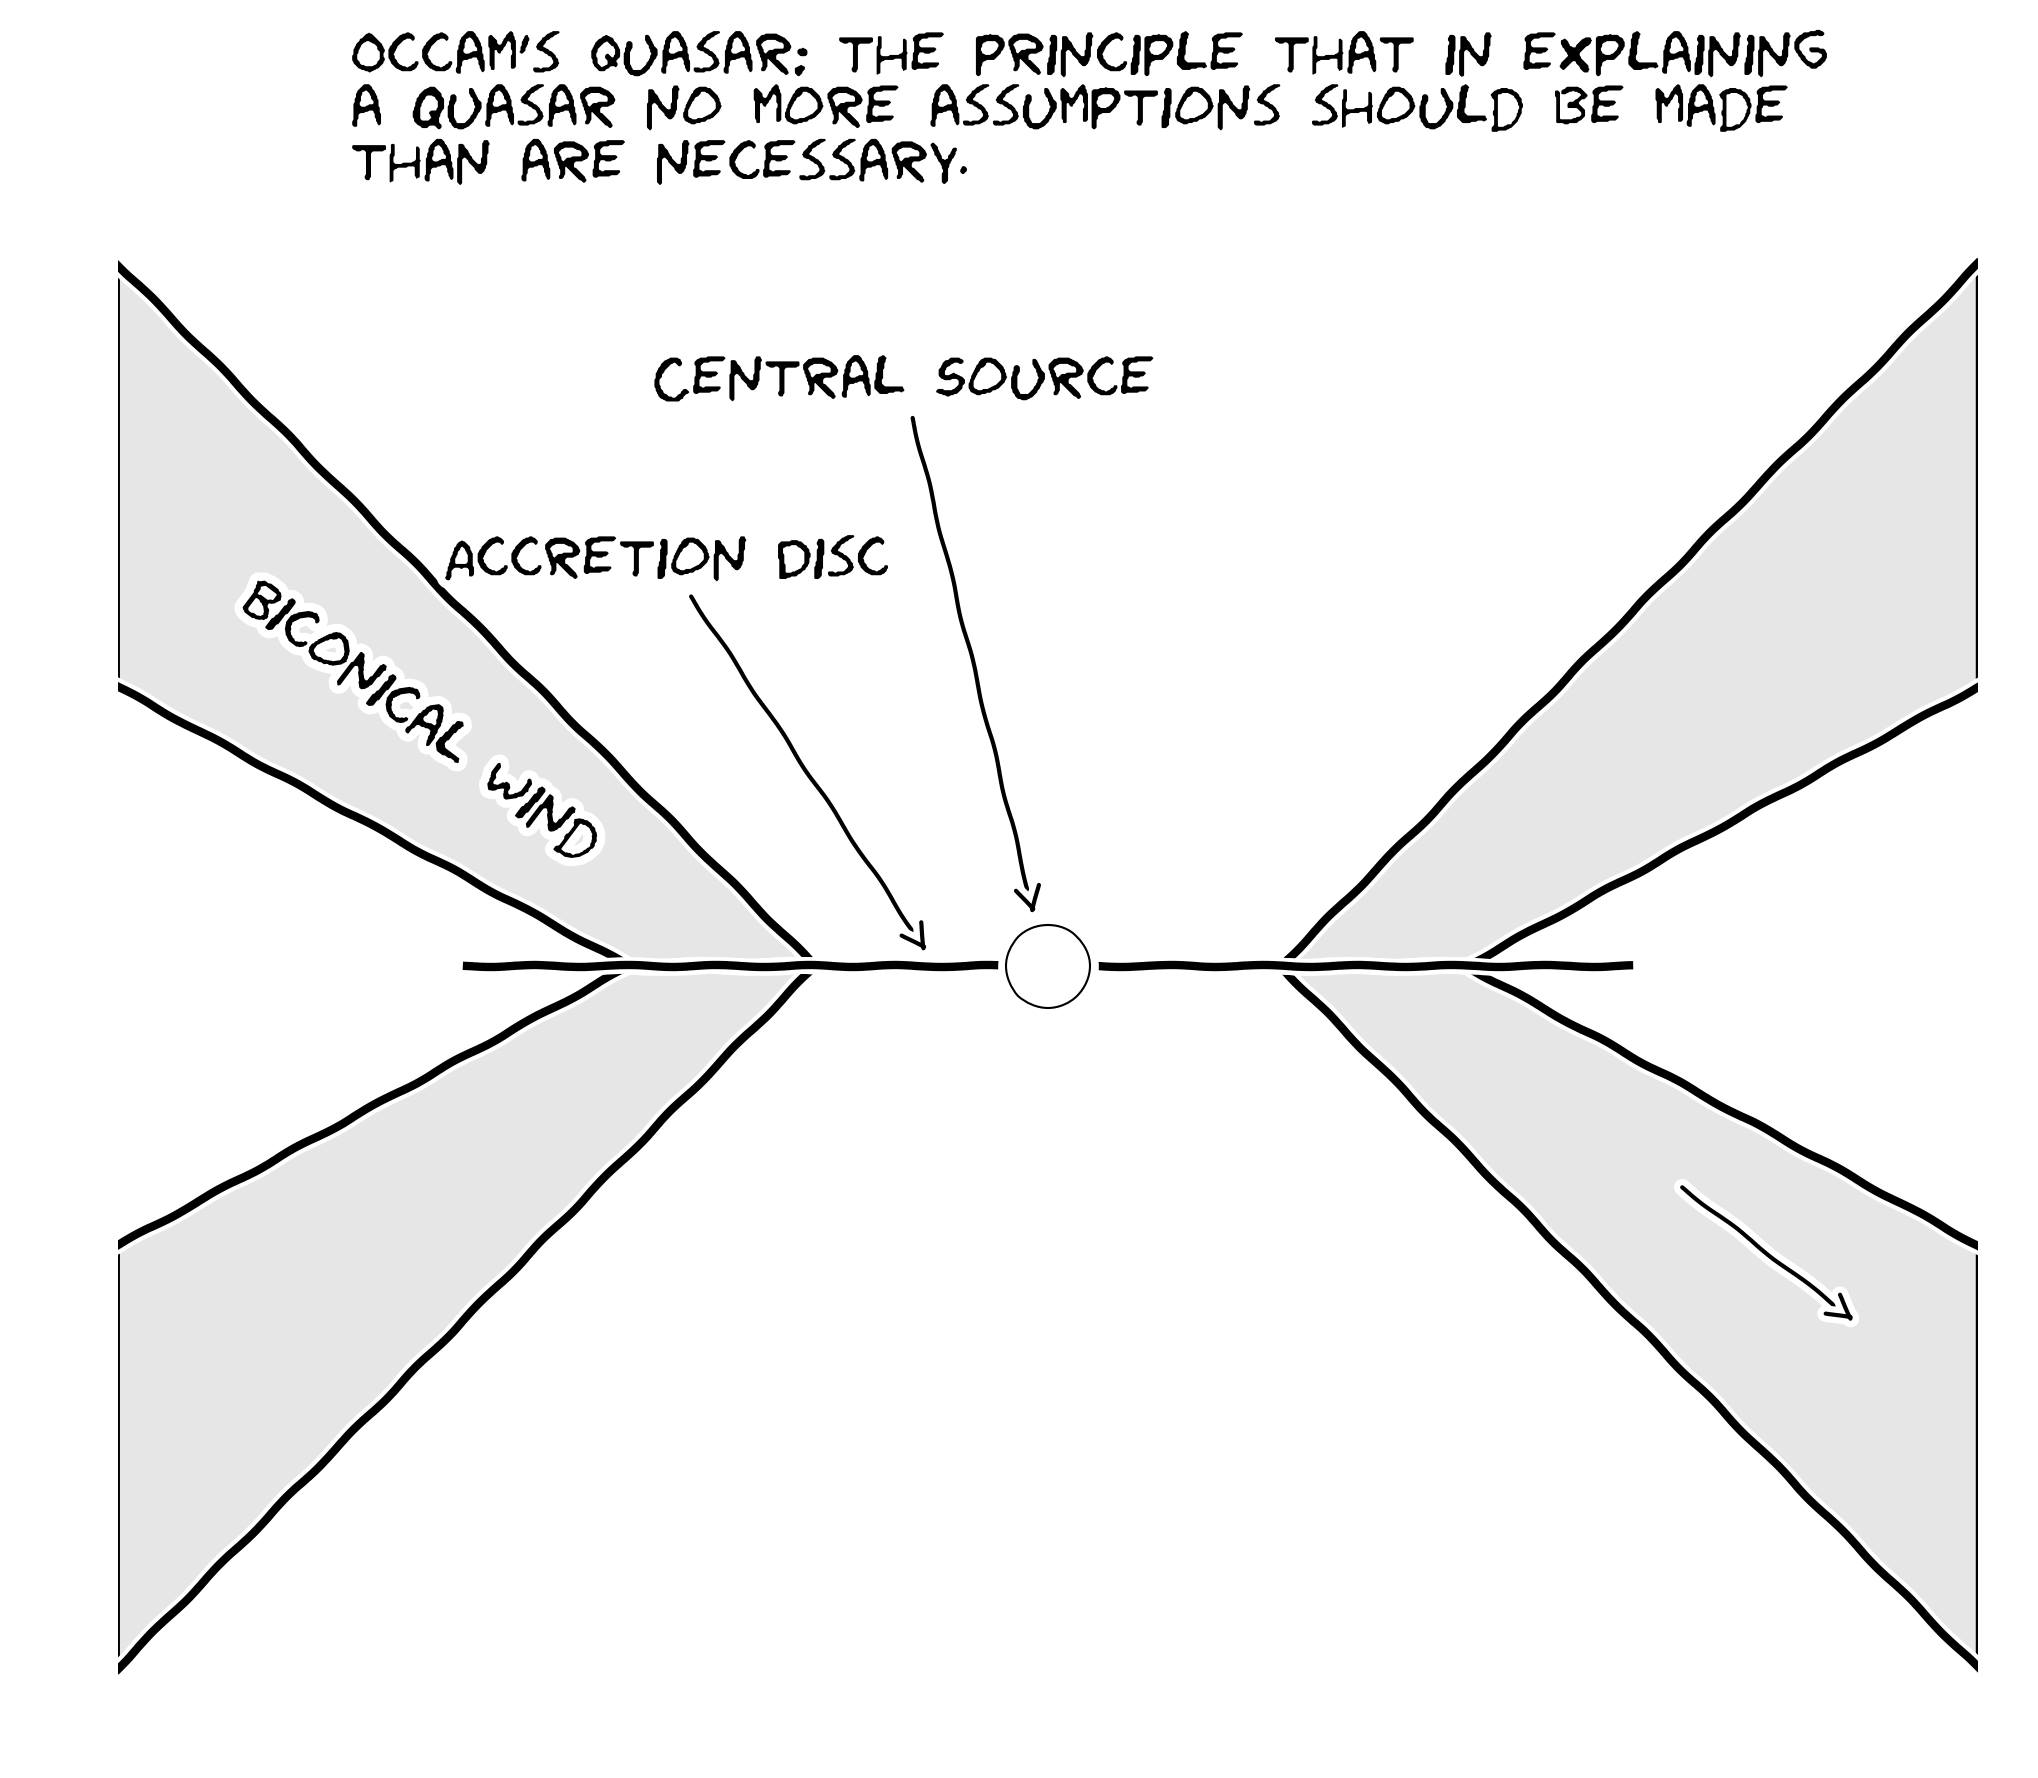
\includegraphics[width=1.0\textwidth]{figures/01-intro/occam.jpg}
\caption
[Occam's quasar]
{
Occam's quasar. How far can this general picture take us when trying to explain
the behaviour of quasars and other accreting compact objects?
} 
\label{fig:occam}
\end{figure}


\section{The Current Understanding of the Disc Continuum}

\label{sec:disc_continuum}

The SS73 model is still the most common way to fit accretion disc spectra and infer
information about the underlying physics. However, 
a number of issues have been raised with the thin-disc model and
its applicability to accreting systems. 

\subsection{The Spectral shape of CV discs}

Attempts to fit the observed SEDs of high-state CVs with simple disc models 
have met with mixed success. In
particular, the SEDs predicted by most stellar/disc atmosphere models 
are too blue in the UV \citep{wade1988,long1991,long1994,knigge1998} and exhibit
stronger-than-observed Balmer jumps in absorption 
\citep{wade1984,haug1987,ladous1989b,knigge1998}. One possible
explanation for these problems is that these models fail to capture
all of the relevant physics. Indeed, it has been argued that a
self-consistent treatment can produce better agreement with 
observational data (e.g. Shaviv et al. 1991;  but see also Idan et al. 2010).
\nocite{idanshaviv2010} \nocite{shaviv1991}
However, an alternative explanation, suggested by Knigge et al.
(1998b; see also Hassall et al. 1985)\nocite{KLWB98,hassall}, 
is that recombination continuum emission from the base of the 
disc wind might fill in the disc's Balmer absorption edge and flatten 
the UV spectrum.

Alternatively, it may just be that CV disks are never really in
a steady state, and so we should only expect the $R^{-3/4}$
temperature profile to hold in a limited portion of the disc.
From eclipse mapping, it has been shown that the inferred accretion
rate increases with radius in NLs \citep{rutten1992, horne1993}.
These results suggest that a non-radiative form of energy loss
is present in the inner regions of the disc, of which potential forms
would be advection or mass loss. This is yet another piece of evidence
that the understanding of accretion and outflow 
are intertwined, although hopefully not inextricably.

\subsection{The Big Blue Bump in AGN}

Does the SS73 model apply well to AGN spectra? There are constrasting views on the matter.
On the one hand, \cite{antonucci2013} claims that ``most of the AGN community is mesmerized by unphysical models that have no predictive power''. 
Yet a recent spectral fitting study by \cite{capellupo2015} concludes that 
``altogether, these results indicate that thin ADs are indeed the 
main power houses of AGN''. So, what are the current problems when 
confronting thin disc models with observation? 

\subsubsection{The Accretion Disc Size Problem}

One of the most interesting results of recent years relating to AGN and accretion discs is
the discovery that the continuum emission region size appears to be
a factor $\sim3$ larger than predicted by standard thin disc theory. This result
has been found independently in both microlensing \citep{morgan2010,dai2010} 
and reverberation \citep{edelson2015} studies, and poses a challenge to the 
current best-bet model for the big blue bump in AGN. 
One proposed solution is that the discs in AGN are inhomogenous,
consisting of individual clumps with independently
varying temperatures \citep{dexteragol2011}, but this is very much
still an active area of research. It is worth noting that the impact
of winds on these results has not yet been properly quantified, something
our team is currently trying to address \citep{mangham}.

\subsubsection{Fitting AGN Spectra and the 1000\AA\ Break}

One of the {\em successes} of the thin disc model, when applied to AGN,
is that we do observe a slope in the UV of $\alpha_{UV} = 0.32$, confirming
the theoretical prediction of $\nu^{1/3}$. 
However, AGN spectra do not exhibit the {\em overall} spectral shape 
\citep[e.g.][]{davis2007,shankar2016} or colour-mass scalings \citep{bonning2007} 
expected from theoretical predictions. 
This can be seen clearly in figure~\ref{fig:agn_templates},
where both the quasar and Seyfert spectra tend to peak in the UV, rather than
the EUV. Furthermore, there is a characteristic break in AGN spectra at
around $1000$~\AA\ \citep{lusso2015}, which does not scale with BH mass or luminosity,
as one might expect for a break associated with an accretion disc. 
There is also no evidence in AGN of the expected polarisation signatures from an 
optically thick disc atmosphere \citep{stockman1979,antonucci1988,antonucci1996}. 

Despite these problems, recent work suggests that the thin disc model 
still has some potential. \cite{capellupo2015} were able to fit a number of
AGN spectra in the UV and optical with thin disc models, although successful fits
were only found once they included effects such as Comptonisation and mass-loss,
as well as correcting for extinction. BH spin also had a reasonable effect on the 
spectral fits, although it is somewhat difficult to constrain from spectral fitting alone.
The $1000$~\AA\ break has also been explained with a mass-losing disc \citep{laordavis2014},
and \cite{lusso2015} suggested that incorrect IGM corrections 
may be exacerbating the effect.
So, while many problems exist, it may not quite be time to 
abandon the Shakura-Sunyaev ship just yet.

\section{The Universality of Accretion}

Accretion appears to be an important physical processes across $\sim10$ orders
of magnitude in mass. But is this process the same on all scales? Does any 
behaviour manifest in all accreting systems? 

\subsection{The RMS-flux relation}

Broad-band variability is common in all types of accretion disc. It has been
known for some time that there exists a linear relationship
between the flux and absolute root-mean-square (rms) amplitude
of this variability. This was discovered first in XRBs and AGN 
\citep{uttley2001, uttley2005, heil2012}, but it has been shown
more recently that the relationship extends to CVs and even YSOs 
\citep{scaringi2012,scaringi2015a}. The relationship is also not limited
to just one type of CV but is present in both NLs and DNe \citep{vandesande2015}.
 
The model that best reproduces this behaviour is the so-called
`fluctuating accretion disc' model \citep{lyubarskii1997,kotov2001,
arevalo2006,hogg2015}. More generally,
additive processes cannot reproduce this behaviour, and a multiplicative
mechanism is required \citep{uttley2005}. 
Regardless of the mechanism, the rms-flux relation is one of the most
clear-cut examples of a universal accretion phenomenon. 
It tells us that at least some of the behaviour in CV discs
is also present in AGN and XRBs, strengthening the argument that CVs
can be used as `accretion laboratories'. 


\subsection{Accretion states and disc-jet coupling}
\label{sec:disc-jet}

Variable and transient sources are common in astrophysics, particularly
when the sources are accreting. I have already mentioned the DIM an
and its applicability to LMXBs and CVs; it turns out that when one plots
the colour and luminosity evolution over the course of an ourburst cycle 
then they follow very similar tracks \
citep[see figure~\ref{fig:kording_hid}, ][]{kordingDNjet2008}.
The detection of radio jets is also intrinsically linked to the accretion state
of the system (disc-jet coupling), as jets only appear in the `hard' accretion 
state, to the right of the so-called `jet line' \citep{fender2001,fender2004}.
\cite{kordingDNjet2008} showed that this behaviour also occurs in CVs, 
as radio emission in the DN SS Cyg is also detected in the same region 
of colour-luminosity space. There is also a well-known correlation between 
radio and X-ray luminosities in low-hard states \citep{gallo2003}.

This clear correlation with accretion state on HIDs has natural parallels 
with AGN. 


The jet production mechanism in BHs in general is not well known. 
Theoretical work suggests that radio jets should be correlated with BH spin 
\citep{penrose1971,blandford1977}, 
but whether such a correlation exists in LMXBs is 
controversial \citep{fender2010,narayan2012}.
This has significant implications for AGN; if powerful radio jets are 
associated exclusively with rotating BHs then the number of radio-loud AGN
would imply a large fraction of them must be rapidly spinning, with
high radiative efficiencies. 
Further evidence that radio jets are not simply produced by RIAFs onto spinning
BHs is found when one considers that NLs show evidence of synchrotron
radio emission \citep{coppejans2015}. This important result suggests that our understanding
of jets is incomplete, and that the links between accretion state and 
jet production are fundamental, but unsolved. Disc winds may complicate, or simplify,
matters, depending on one's outlook (see chapter 2).

\begin{figure}
\centering
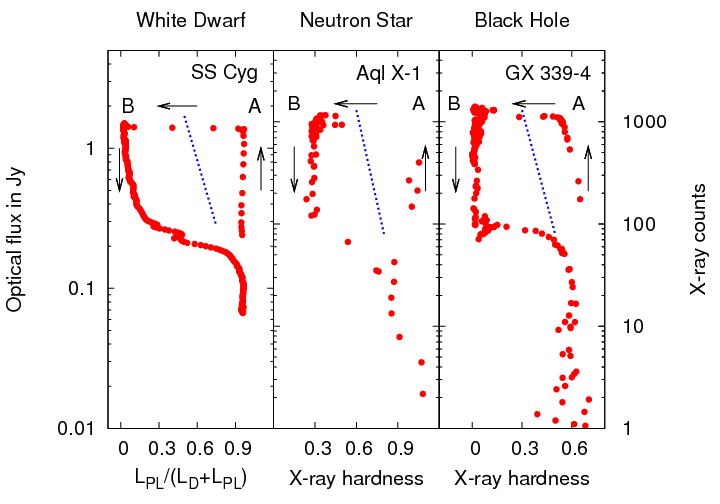
\includegraphics[width=1.0\textwidth]{figures/01-intro/kording_hid.png}
\caption
[Hardness-intensity diagrams for three types of accreting objects.]
{
{\sl Credit: Kording et al. 2008.} 
Caption.
} 
\label{fig:kording_hid}
\end{figure}

\subsection{A Global Picture}

Clearly, accretion physics is relevant to a plethora of astrophysical phenomena, 
and at least some of the physics of accretion is applicable to {\em all} 
classes of accreting object. 
It would also appear that the outflowing material observed in accreting systems 
has a profound effect on the accretion process itself, and 
possibly significantly affects the observational 
appearance of disc-accreting systems (c.f. Elvis unification model). 
Hence, in the next chapter, I will review the evidence for
winds and discuss some of the relevant background theory.

 % Introduction

\newpage
\lhead{\emph{2. Accretion Disc Winds}}  % Set the left side page header to "Contents"
 \chapter{Accretion Disc Winds}
\label{sec:winds}

\epigraph{``A view of space, with an elephant obstructing it"}
{{\sl Mike Vennart, Silent/Transparent}}


%%%%WINDS 
%%% COULD MAKE THIS A NEW CHAPTER
\section{Observational Evidence}

\index{outflows!observational evidence}
Observational evidence for mass-loaded outflows or winds is 
widespread across the entire astrophysical mass range and most of
the electromagnetic spectrum. Before exploring this evidence, 
it is pertinent to briefly discuss the `smoking gun'
used to unambiguously detect winds -- the presence of blue-shifted BALs
or `P-Cygni' profiles in an object's spectrum. 
\index{P-Cygni profile}

\begin{figure}
\centering
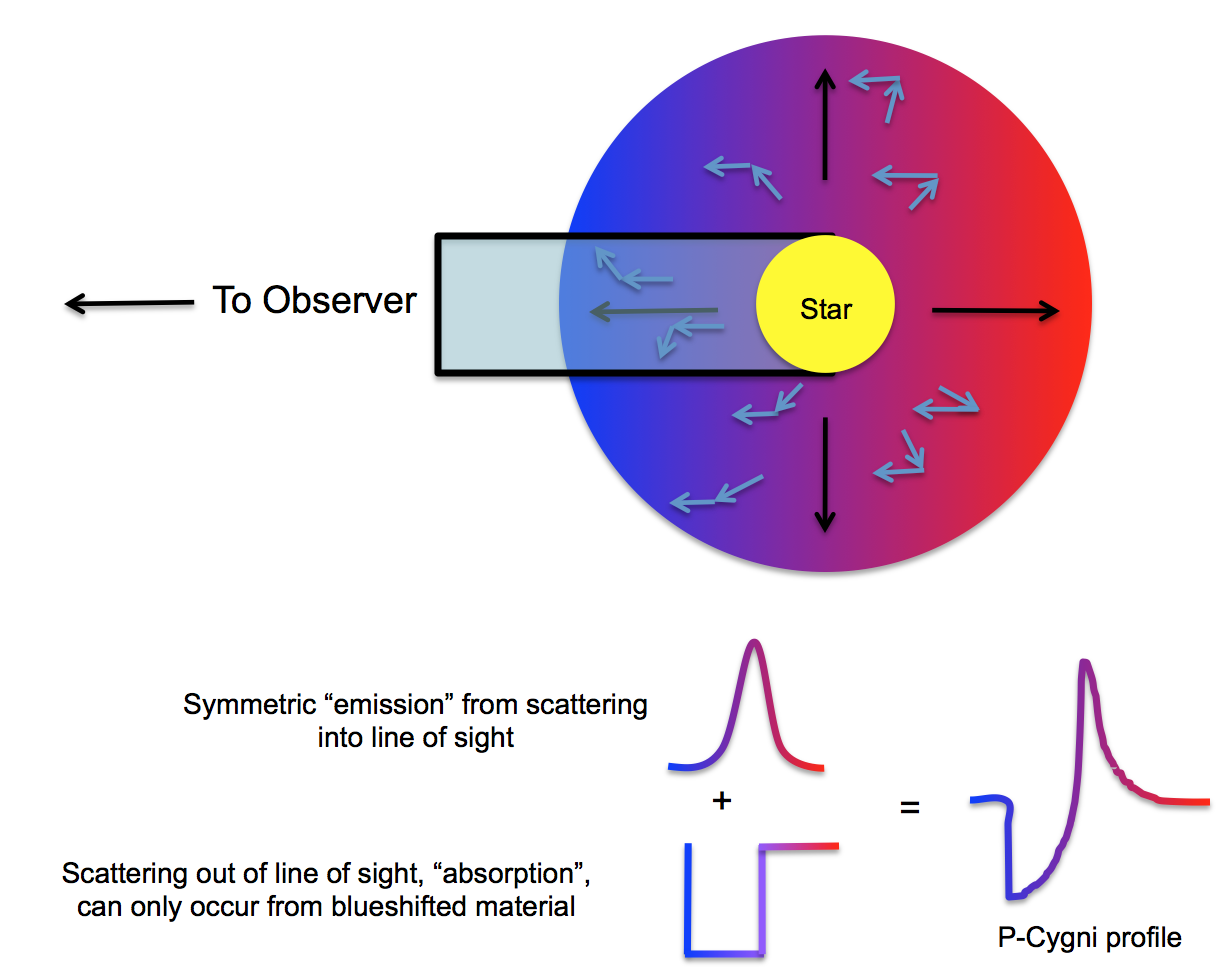
\includegraphics[width=1.0\textwidth]{figures/02-outflows/pcyg.png}
\caption
[A disagram showing how P-Cygni profiles form.]
{
Diagram showing how an expanding envelope or wind presenting significant line
opacity around a continuum source leads to the formation of P-Cygni profiles.
The black arrows denote the outflow direction and the blue arrows typical
scattering interactions.
} 
\label{fig:pcyg}
\end{figure}

Fig.~\ref{fig:pcyg} shows how a spherical outflow presenting\index{outflows!spherical}
significant line opacity will 
cause these characteristic profile shapes to form, 
as scattering out of the line of sight 
causes a dip in the blue wing of the line, while scattering into the 
line of sight from other portions of the outflow causes an increase in flux
in the red wing of the line. The situation is much more complex in most
astrophysical situations; for example, the geometry is rarely spherically 
symmetric, and the line is rarely a pure scattering case. 
Indeed, the potential 
for complicated radiative transfer effects and 
the variety in line formation mechanisms 
(e.g. recombination, collisional excitation)
is one of the reasons why 3D Monte Carlo radiative 
transfer simulations are necessary
to effectively model disc winds (see chapter 3).



\subsection{Cataclysmic Variables}
\label{sec:cv_winds}
\index{cataclysmic variable}\index{cataclysmic variable!winds}
It has been known for a long time that winds emanating from
accretion discs are important in shaping the ultraviolet (UV) spectra
of high-state CVs \citep{heap1978, greensteinoke1982}. 
The most spectacular evidence for such
outflows are the P-Cygni-like profiles seen in UV resonance lines such as
\civfull\ \citep[e.g. ][see Fig.~\ref{fig:cordova}]{cordova1982}. 
Considerable effort has been spent over the
years on understanding and modelling these UV features 
\citep[e.g.][]{drewverbunt1985,maucheraymond1987,SV93,KWD95,
kd1997,knigge1997,LK02,noebauer,puebla2011}. 
The basic picture emerging from these efforts is
of a slowly accelerating, moderately collimated bipolar
outflow that carries away $\simeq 1\% - 10\%$ of the accreting
material. State-of-the-art simulations of line formation in this type
of disc wind can produce UV line profiles that are remarkably similar
to observations, as shown in Fig.~\ref{fig:zcam_lk02}.

\begin{figure}
\centering
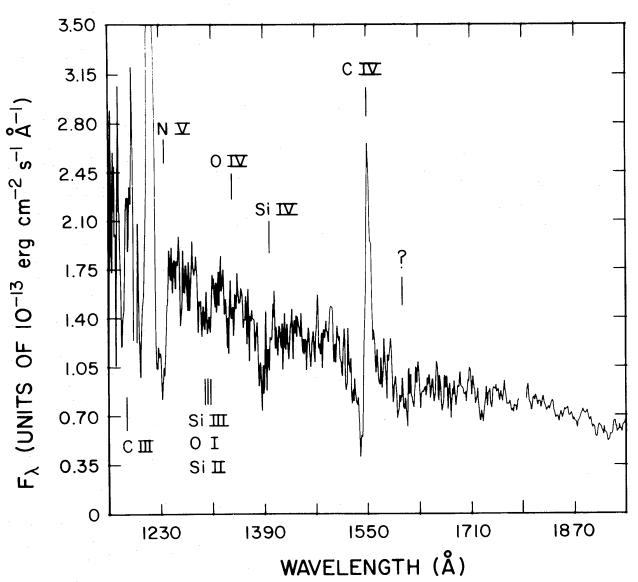
\includegraphics[width=0.8\textwidth]{figures/02-outflows/cordova_mason.png}
\caption
[UV spectrum of the DN TW Vir during outburst.]
{
{\sl Credit: Cordova \& Mason 1982}. 
UV spectrum of the DN TW Vir during outburst. The P-Cygni profiles
can be seen clearly, demonstrating that a strong, fast outflow is present
in the system. 
} 
\label{fig:cordova}
\end{figure}

\begin{figure}
\centering
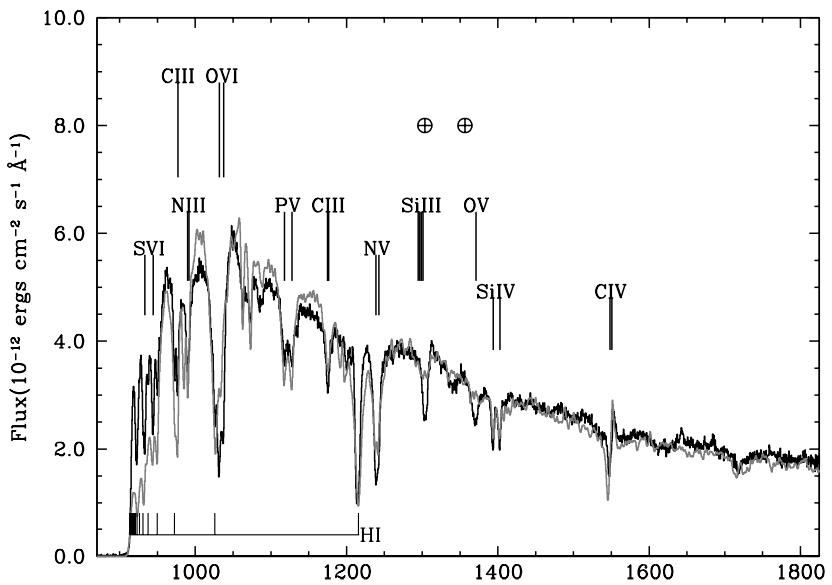
\includegraphics[width=0.8\textwidth]{figures/02-outflows/zcam_lk02.png}
\caption
[UV spectrum of Z Cam, compared to a synthetic spectrum from MCRT simulations.]
{
{\sl Credit: Long \& Knigge 2002}. 
UV spectrum of Z Cam (black), compared to a synthetic spectrum from MCRT simulations (grey).
} 
\label{fig:zcam_lk02}
\end{figure}

\begin{figure}
\centering
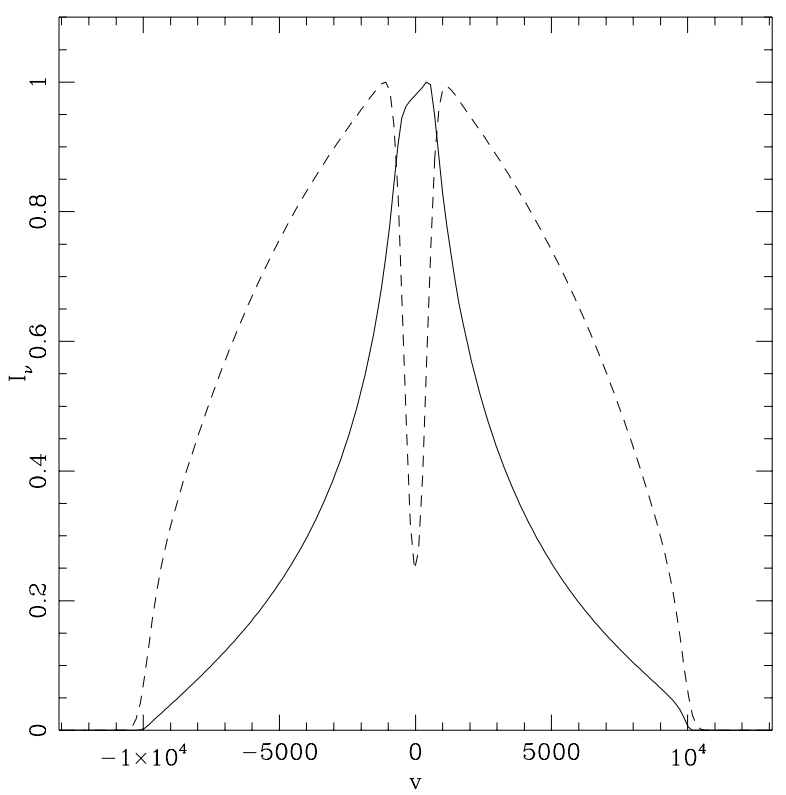
\includegraphics[width=0.7\textwidth]{figures/02-outflows/mc_line.png}
\caption
[The effect of a disc wind on a double-peaked line profile.]
{
{\sl Credit: Murray \& Chiang (1997)}. 
A comparison between a line profile, normalised to have peak intensity of 1,
produced from a Keplerian disk (solid line) and the same model with an additional
disc wind (dashed line). The radial velocity component of the disc wind modifies
the escape probabilities across the disc, causing a single-peaked line to form.
} 
\label{fig:mc_line}
\end{figure}

Much less is known about the effect of these outflows on the optical
spectra of high-state CVs. Direct evidence of wind-formed lines comes from
isolated observations of P-Cygni-like line profiles in
\ha\ and He \textsc{i} $5876$~\AA, 
\citep{patterson1996, RN98, kafka2004}. 
However, the effect of a wind  on the {\em emission} lines in the optical\index{emission line}
spectrum is unclear.
\cite{MC96, MC97} have shown that the presence of disc winds may
offer a natural explanation for the single-peaked optical emission lines in\index{emission line!single-peaked}
high-state CVs, since they can strongly affect the radiative transfer
of line photons \citep[Fig.~\ref{fig:mc_line}; also see][]{flohic2012}. 
Stronger support for a significant wind contribution to the
optical emission lines comes from observations of eclipsing
systems. There, the single-peaked lines are often only weakly
eclipsed, and a significant fraction of the line flux remains visible
even near mid-eclipse \citep[e.g.][]{baptista2000,groot2004}. 
This points to line formation in a spatially
extended region, such as a disc wind.
It is also possible that a wind may affect the continuum emission of CVs,
as described in section~\ref{sec:disc_continuum}. 
The effect of an accretion disc wind
on the optical line and continuum emission of CVs is addressed directly
in chapter 4.

\subsection{X-ray Binaries}
\label{sec:xrb_winds}

\index{X-ray binary}
As in CVs, evidence for fast outflows in LMXBs is not constrained to 
a single waveband. UV absorption in outflows was detected when
\cite{ioannau2003} observed \civfull\ P-Cygni profiles with blueshifts 
of $\sim1500$~km~s$^{-1}$ in the LMXB X2127+119.\index{P-Cygni profile} 
A series of studies also found X-ray absorption features in similar objects 
\citep{ueda1998,kotani2000,parmar2002}.\index{X-ray binary!low mass} 
These absorption features appeared to be preferentially detected
in `dipping' LMXBs. Dips in X-ray flux are thought to occur
in systems with inclinations $\gtrsim70^\circ$ 
\citep{vanderhooft1998,tanaka2003,church2005}, and possible explanations
involve disc precession \citep{barnard2006,shaw2013},\index{absorption line}  
failed state transitions \citep{soleri2013,shaw2016} or low ionization material 
partially covering the X-ray source \citep{tanaka2003}.\index{iron line}\index{accretion!state}
\cite{ponti2012} confirmed that broad absorption in highly ionized Fe lines 
occurred only in the dipping LMXBs in their sample and proposed an equatorial 
outflow geometry based on this association (see Fig.~\ref{fig:ponti_cartoon}). 
The same study also demonstrated that the winds only appeared in the soft, 
disc dominated accretion state, on the opposite side of the HID to the
region where jets are common (Fig.~\ref{fig:ponti_hid}). 
This exciting result illustrates how
important winds are to our understanding of accretion and requires that
we expand the discussion of accretion states from `disc-jet' coupling
to also include winds.

\begin{figure}
\centering
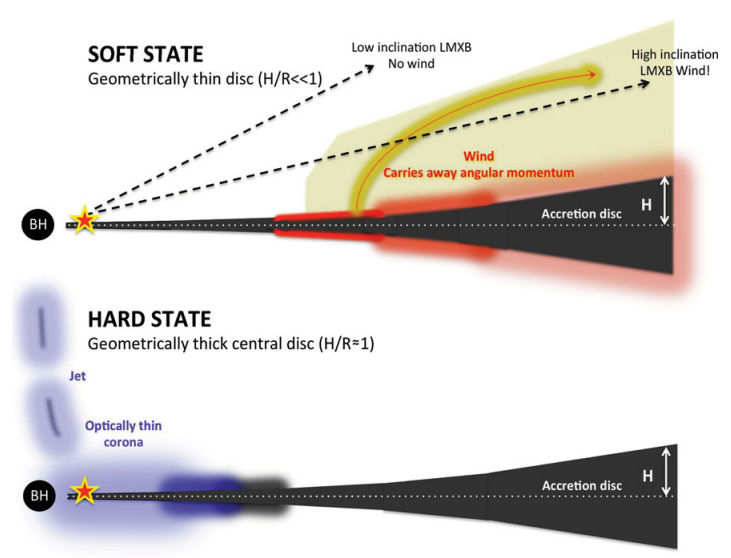
\includegraphics[width=0.8\textwidth]{figures/01-intro/ponti_wind_cartoon.png}
\caption
[A cartoon illustrating the expected geometry of soft-state LMXB winds.]
{
{\sl Credit: Fig. 3, Ponti et al. 2012, ``Ubiquitous equatorial accretion disc winds in black hole soft states'', MNRAS letters, 422, 11.
}. 
A cartoon illustrating the expected geometry of the disc and outflows in
LMXBs in the soft and hard states.
} 
\label{fig:ponti_cartoon}
\end{figure}


\begin{figure}
\centering
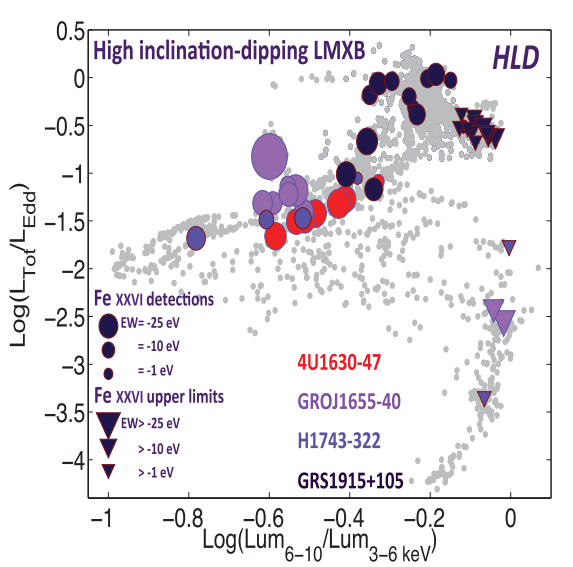
\includegraphics[width=0.8\textwidth]{figures/02-outflows/ponti_hid_dip.png}
\caption
[Hardness-intensity diagram for four dipping LMXBs.]
{
{\sl Credit: Fig. 2, Ponti et al. 2012, ``Ubiquitous equatorial accretion disc winds in black hole soft states'', MNRAS letters, 422, 11.
}. 
Hardness-luminosity diagram for four dipping LMXBs,
demonstrating that winds appear only in the soft state. 
The points are colour-coded by system, and are shown against the 
background grey points of all LMXBs studied by Ponti et al. (2012).
None of the low inclination sources in their sample show Fe~\textsc{xxvi}
absorption detections.
} 
\label{fig:ponti_hid}
\end{figure}


\subsection{AGN and Quasars}
\label{sec:agn_winds}

\subsubsection{Broad Absorption Line Quasars}
\label{sec:balqsos}

\begin{figure}
\centering
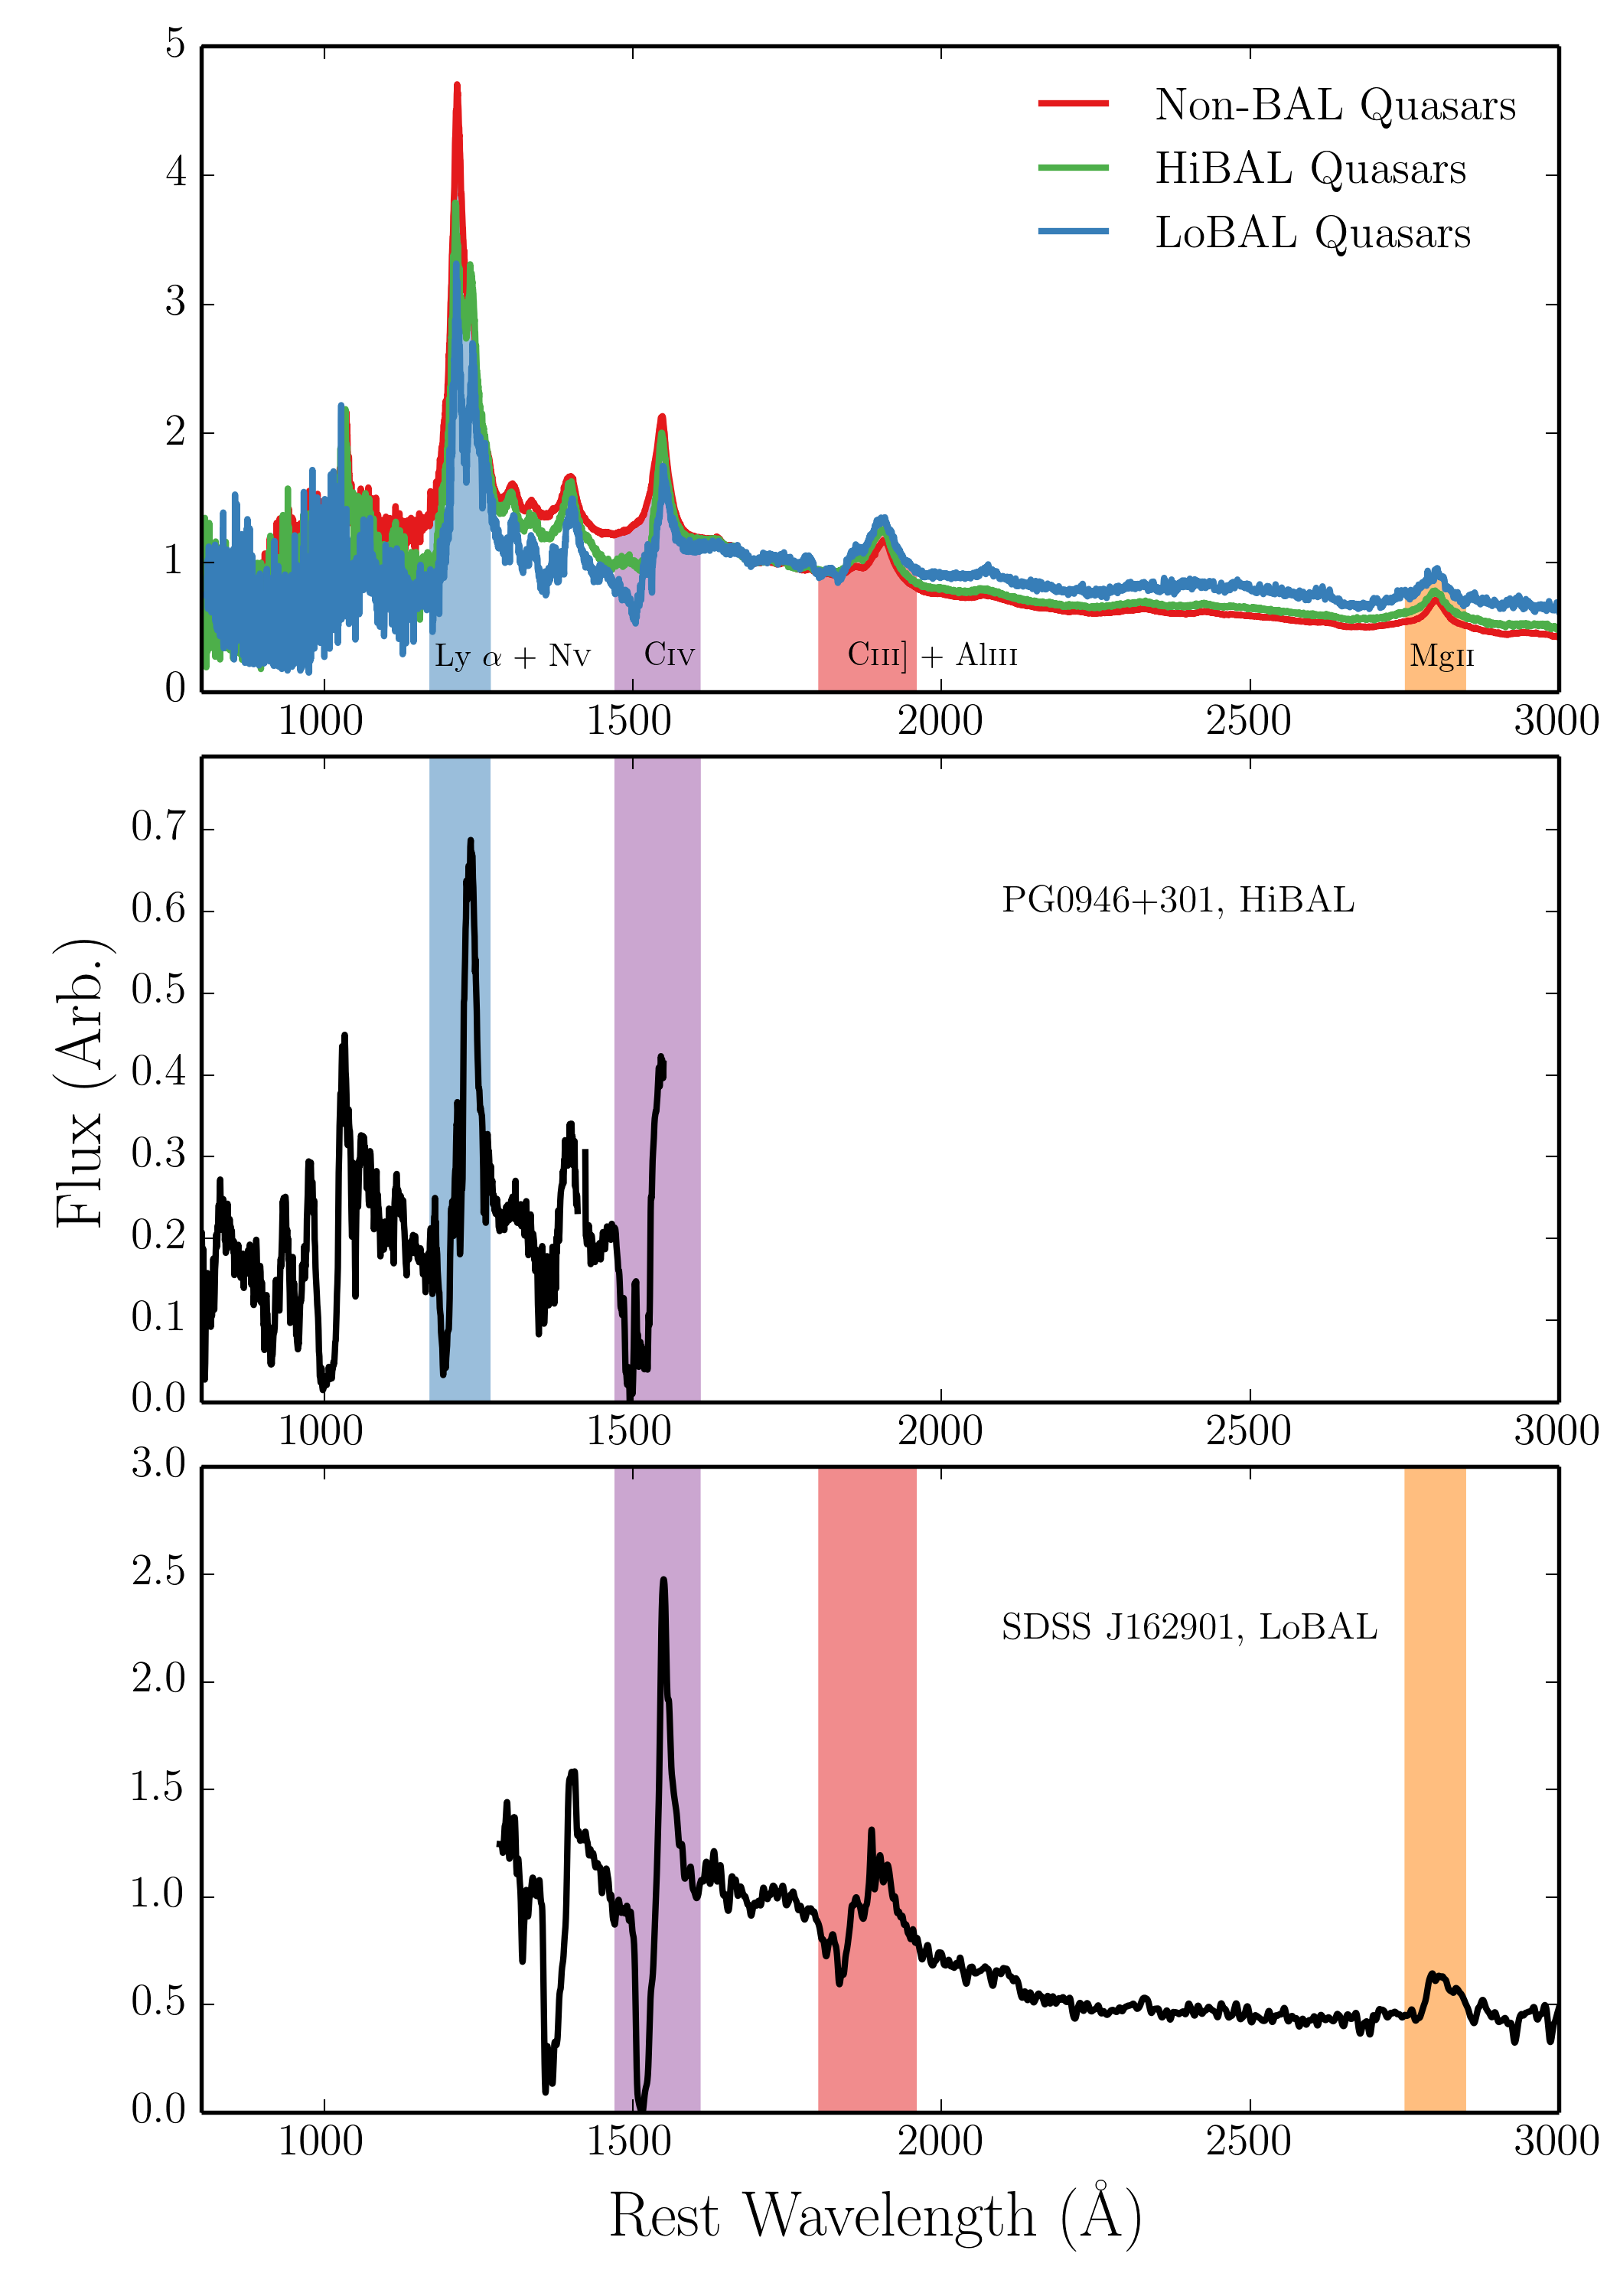
\includegraphics[width=1.0\textwidth]{figures/02-outflows/bal_spectra.png}
\caption
[Some example non-BAL, HiBAL and LoBAL spectra.]
{
Top Panel: A comparison between the SDSS non-BAL, HiBAL and LoBAL
composite spectra as presented in \cite{reichard2003}. 
Bottom Two Panels: Two individual examples of a HiBAL and LoBAL quasar
spectrum, respectively. In all panels some of the more prominent
lines are labeled and shaded, and the object name is given in 
the bottom two plots.
} 
\label{fig:bals}
\end{figure}
\index{BALQSOs}\index{quasar}\index{absorption line}\index{disc wind}
Perhaps the clearest evidence of outflows in AGN is provided by  
the blueshifted ($\sim 0.1~c$) ultraviolet 
BALs seen in approximately $20\%$ of quasars
\citep{weymann1991, knigge2008, dai2008, allen2011}. 
High-ionization BAL quasars (HiBALs)\index{BALs}\index{BALQSOs}
only show broad, blue-shifted absorption in species such as 
\civ, Si~\textsc{iv}, \nv\ and \ovi, the most prominent BAL
profile often being associated with the \civline\ line.
In addition to the more common HiBALs, 
approximately $10\%$ of BALQSOs also show absorption
in lower ionization species such as \mgii\ and \aliii\ 
\citep[LoBALs;][]{voit1993,gibson2009};
an even smaller subset also show absorption in Fe~\textsc{ii} and 
\textsc{iii} \citep[FeLoBALs;][]{becker2000,hall2002}. 
Some example spectra of BAL quasars from the HST and SDSS archives are shown in 
Fig.~\ref{fig:bals}, with important spectral lines marked.
\index{Hubble Space Telescope}\index{SDSS}\index{BALs}\index{absorption line}

The simplest explanation for the incidence of 
BAL quasars (BALQSOs) is in terms of an accretion disc wind viewed
from different angles. This principle of geometric unification
is very similar to the idea behind the UP95 and AM95 models discussed in Chapter 1.
According to this paradigm, a biconical wind rises from 
the accretion disc so that the BALQSO fraction is associated with
the covering factor of the outflow. This fraction
has been estimated by various authors using different 
selection criteria, with 
values ranging between $10\%$ and $40\%$ depending on the treatment 
of selection effects and the classification scheme used 
\citep{weymann1991, trump2006, knigge2008, dai2008, allen2011}.

BAL quasars can also be interpreted in an {\em evolutionary}
context, in which quasars spend a certain proportion of their life
in the `BAL phase'. Models generally put this phase near the start
of the quasar lifetime \citep{hazard1984,surdej1987,boroson1992,zubovas2013}, 
after a dust-enshrouded phase, but before
the main quasar period. It is perhaps more likely that {\em both} 
evolutionary and geometric effects are at work \citep{borguet2010,dai2012}.
One of the main problems with testing these two paradigms is that many of
the properties of BAL quasars fit naturally into either picture, and so
disentangling their true nature is challenging. 
The latter chapters of this thesis attempt to address this issue by testing the 
geometric unification model
and seeing how close this simple picture can get to explaining 
the BAL phenomenon.  


The BAL fraction, $f_{BAL}$, is a very useful number and must be at least
related to the covering factor of the outflow. However, selection effects associated
with the reduction in flux by the BALs themselves \citep{knigge2008} and enhanced 
reddening/extinction in BALQSOs \citep{reichard2003,allen2011}
could lead to significant underestimates of $f_{BAL}$. 
The angular dependence of the continuum causes further problems,
as objects viewed from higher inclinations could be severely under-represented in 
a flux-limited sample \citep{goodrich1997,krolikvoit1998}.
Unfortunately, accurately correcting for these effects is difficult. 
The degree of collimation of the BAL wind
is also not well known. Polarisation studies suggest that the\index{polarisation}
wind is roughly equatorial \citep{goodrich1995, cohen1995}, 
as also found from hydrodynamical and radiative transfer simulations 
\citep{PSK2000,PK04, higginbottom2013, borguet2010}.
However, there is also evidence for polar BAL outflows in 
radio-loud (RL) sources \citep{zhou2006,ghoshpunsly2007}.
In addition to these uncertainties, the physical scale of the BAL
phenomenon is also disputed and may vary from object to object.
A common assumption is that the BAL region is roughly co-spatial with
the BLR, which is reasonable considering the similar velocity widths
and ionization states in BELs and BALs. In this case, 
the radius of the absorbing material
can be estimated as $\sim 100~r_G -1000~r_G$ from reverberation mapping
and microlensing \citep[e.g., for BLRs in BALQSOs,][]{sluse2015,odowd2015}.
However, distances of  $\sim0.1$~pc ($\sim 10^4~r_G$) 
have been estimated in at least some objects from photionization modelling, 
conducted using densities calculated from absorption line doublets
\citep{borguet2013,chamberlain2015}.\index{absorption line}

BAL quasars display a wide variety of different trough shapes. 
The line profiles themselves often show complex structure 
\citep{foltz1987,ganguly2006, simonhamann2010} and can be time variable 
\citep{hall2011, capellupo2011,capellupo2012,capellupo2014, filizak2012}. 
Furthermore, a subset of quasars show
BAL-like absorption troughs with much smaller velocity widths. Depending 
on their width, these are known as narrow absorption lines (NALs) or `mini-BALs'
\citep{misawa2007,misawa2008,nestor2008}.
While some of this behaviour can be explained once again as a viewing angle
effect \citep[e.g. ][]{ganguly2001}, the
BAL profile variety and variability implies that BALQSOs 
are far from a homogenous population, and perhaps suggests the existence of
dense substructures (clumps) in their flows. Such clumpiness has been invoked
in several disc wind unification models for AGN and quasars
(see section~\ref{sec:wind_models})\index{clumping}

The X-ray properties of BAL quasars are particularly important due
to the strong ionizing potential of the X-ray radiation. 
Observationally, BALQSOs are X-ray weak when compared to 
non-BAL quasars \citep{gibson2009}. 
This X-ray weakness is often attributed to the presence of absorbing material
with column densities of $N_H \sim 10^{22-24}$~cm$^{-2}$ along the line of sight
\citep{gallagher1999,gallagher2002,green2001,grupe2003,stalin2011},
although there is also evidence that BALQSOs are {\em intrinsically}
X-ray weak \citep{sabra2001,clavel2006,morabito2013}.
The X-ray properties of BAL quasars are fundamentally coupled to 
the properties of the wind -- the X-ray absorption may, in fact, be caused by 
the outflow, which in turn has its ionization state 
determined by the X-ray radiation. Furthermore, the true X-ray 
luminosities cannot be reliably inferred until the 
inclinations of BALQSOs are
constrained, as gravitational lensing can significantly alter the
emergent angular distribution of X-ray emission even for an intrinsically
isotropic source \citep{chen2013a, chen2013b}.

Although the observed X-ray emission in BALQSOs is weaker than in otherwise similar
quasars, it still still possesses strong ionizing power. This leads to what has become
known as the `over-ionization problem' in BALQSOs: how is the moderate 
ionization state of the BAL gas maintained in the presence of ionizing 
X-rays? A number of potential solutions have been proposed, which can be 
broadly separated into `shielding' models \citep{MCGV95,PK04} and `clumpy'
models \citep{dekool1995,hamann2013}. Some of these models are discussed
further in section~\ref{sec:wind_models} and chapter~5.

\subsubsection{Warm Absorbers}

\index{warm absorber}
Warm absorbers (WAs) are regions of photoionized plasma responsible for some
of the characteristic absorption features seen in the 
soft X-ray spectra of AGN \citep{reynolds1995}.
In particular, they produce photoelectric continuum absorption 
\citep[e.g.][]{halpern1984,cappi1996,kriss1996}
and a series of narrow absorption lines in H-like and He-like ions of 
C, N, O, Si, Ne, and Fe \citep{kaastra2000}.
A wind origin is a common hypothesis for WAs 
\citep[e.g.][]{krolikkriss2001}. Clear evidence for this 
comes from the measured blueshifts of the lines, typically on the order of 
a few $100$~km~s$^{-1}$ \citep[e.g.][]{kaastra2000}. X-ray absorption and WAs are often
variable \citep{fabian1994,otani1996}, which may be interpreted in terms of 
the changing kinematics of an accretion disc wind \citep{connolly2014}. 
There is also evidence of contemporary and associated UV and X-ray absorption 
in NGC 5548 \citep{kaastra2014} and in mini-BALS \citep{giustini2011},
and, as mentioned above, BALQSOs often show strong X-ray absorption. 
A number of other AGN also show simultaneous absorption in their X-ray 
and UV spectra \citep[e.g.][]{crenshaw2003,crenshaw2012}, 
although can often arise from absorbers that are not directly associated.
Overall, there is evidence that the same outflow may produce observational signatures  
across a large range of ionization states and line energies. 

Some WAs can be modelled well with single absorbers \citep{kaastra2000}, 
but most require multiple absorption components with different ionization states
\citep[e.g.][]{kriss1996,orr1997,krolikkriss2001,connolly2014}.
One common way to parameterise the ionization state of a plasma is 
via an ionization parameter proportional to the ionizing luminosity, 
given by \citep[e.g.][]{reynolds1995}\index{ionization parameter}
\begin{equation}
\xi = \frac{L_{H}}{n_H R^2},
\label{eq:xi}
\end{equation}\index{ionization parameter}
where $L_H$ is the luminosity above $13.6$eV, and $n_H$ is the number
density of H atoms. If the absorber is stratified and the SED subject to absorption, 
self-consistent ionization and radiative transfer models
should really be used to model the spectrum (see e.g. chapter 3). This is 
because optically thin ionization parameter estimates will not properly capture 
the ionization physics due to the variation of the SED shape within the medium.
The overall body of observations points towards an outflow with a 
stratified ionization structure ranging from 
$\log (\xi / \mathrm{erg~s^{-1}~cm}) \sim 0-2$ 
and densities on the order of $10^7$~cm$^{-3}$, located at around $\sim10^{16}$~cm. 
These physical conditions or scales are not well constrained, and the connection to 
other outflows, such as the ultra-fast outflows introduced in the next section, 
is unknown. Timing observations may help to shed light on 
the properties of the mysterious, but ubiquitous, 
AGN WAs \citep{silva2015}.

\subsubsection{Ultra-fast Outflows}
\label{sec:ufos}

\index{ultra-fast outflow}
In addition to acting as WAs, winds can also imprint clear absorption features
in highly ionized Fe~K$\alpha$ lines in AGN such as PDS~456 
\citep{reeves2003, gofford2014,matzeu2016},
MCG-5-23-16 \citep{braito2007} and PG 1211+143 \citep{poundsreeves2009,fukumura2015}.
These outflow signatures are fairly common in Seyfert galaxies \citep{tombesi2010a, gofford2013}. 
One example of such a feature is shown in 
Fig.~\ref{fig:nardini}, along with a simple spherical outflow model fit 
\citep{nardini2015}. The high velocities ($\sim0.1c$) inferred 
from the line blueshifts have lead to these winds becoming known as 
ultra-fast outflows, or UFOs. 

UFOs are characterised by ionization parameters in the range\index{ionization parameter} 
$\log (\xi / \mathrm{erg~s^{-1}~cm}) \sim 3-4$
and column densities $N_H > 10^{22}$~cm$^{-2}$. Their high mass-loss rates
and large energy budgets mean that they are natural candidates for
AGN feedback (see section~\ref{sec:agn_feedback}). Measurements of
their kinetic luminosities suggest that UFOs have sufficient 
energy to affect their host galaxy \citep{gofford2015}. In fact, 
a large-scale molecular outflow has recently been detected in one 
UFO host, possibly driven by the UFO itself \citep{tombesi2015}. 
As with WAs, many of the models
used to constrain physical parameters are simplistic, and assume 
single ionization parameters, large covering factors
and thin expanding shells of outflow.
Under the assumption of a thin expanding shell, 
the mass-loss rate can be estimated using
\citep[e.g.][]{borguet2012}
\begin{equation}
\label{eq:hse}
\dot{M_W} \sim \Omega \mu N_H m_p v_{\mathrm{out}} R_{\mathrm{out}},
\end{equation}
where $\Omega$ is the solid angle covered by the outflow, $N_H$
is the column density, $m_p$ is the proton mass, $\mu$ is the mean molecular weight,
$v_{\mathrm{out}}$ is the outflow velocity
and $R_{\mathrm{out}}$ is the radius of the shell, often approximated as the launch radius
of the outflow. In reality, the absorber is probably much more complex, and full 
RT and photoionization simulations are required to accurately model 
the expected spectrum. 
In a series of papers, 
\cite{simlong2008,sim2010_hydro,sim2010_hydro} carried out such calculations
and found that reasonable verisimilitude with Fe line profiles could be achieved.
However, as with many models of AGN, a holistic, broad wavelength range
fit is still required.

\begin{figure}
\centering
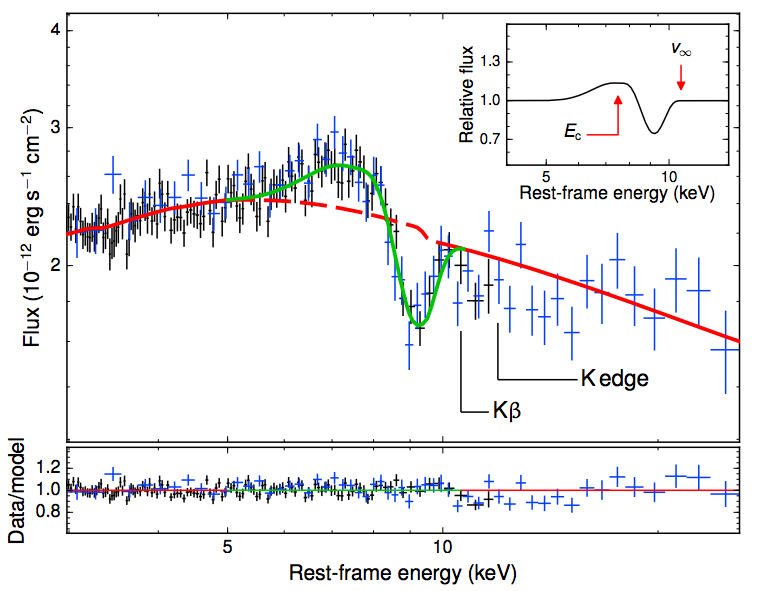
\includegraphics[width=1.0\textwidth]{figures/02-outflows/nardini_pds456.png}
\caption
[X-ray spectrum of PDS 456 fitted with a P-Cygni profile.]
{
{\sl Credit: Fig.3, Nardini et al. 2015, Science, 347, 860. Reprinted with permission from AAAS.}. 
X-ray spectrum of PDS 456 fitted with a P-Cygni profile from a 
spherical outflow model. {\sl XMM-Newton} data is shown in black 
with two combined {\sl NuStar} observations in blue.
} 
\label{fig:nardini}
\end{figure}


\subsection{Stellar Winds}

\label{sec:stellar_winds}
\index{stellar wind}
Although stellar winds are clearly not accretion disc winds,
they provide a useful, and better understood, testing ground for much
of the physics of radiatively-driven outflows. 
Wolf-Rayet (WR) stars and O-stars possess strong outflows with mass-loss rates
of up to $10^{-5}~M_\odot~$yr$^{-1}$, thought to be driven by radiation pressure
mediated by spectral lines (see section~\ref{sec:line_driving}). 
Over the typical lifetime of a massive
star ($\sim10^6$~yr), this can have a significant impact on the overall stellar mass,
causing losses of around $10~M_\odot$ of material. 

As with the systems described previously, the P-Cygni profiles
seen in hot, massive stars provide the key evidence for the presence of
a strong wind (see Fig.~\ref{fig:hot_star_wind}). Mass-loaded
winds are also thought to be responsible for the emission lines 
seen in hot star spectra \citep[e.g.][]{pauldrach1994}. Indeed, emission
line diagnostics have been particularly important in determining
the mass-loss rates of stellar winds and have also been used to demonstrate 
that line-driven stellar winds are clumpy.\index{P-Cygni profile}\index{clumping}\index{line-driving} 

\begin{figure}
\centering
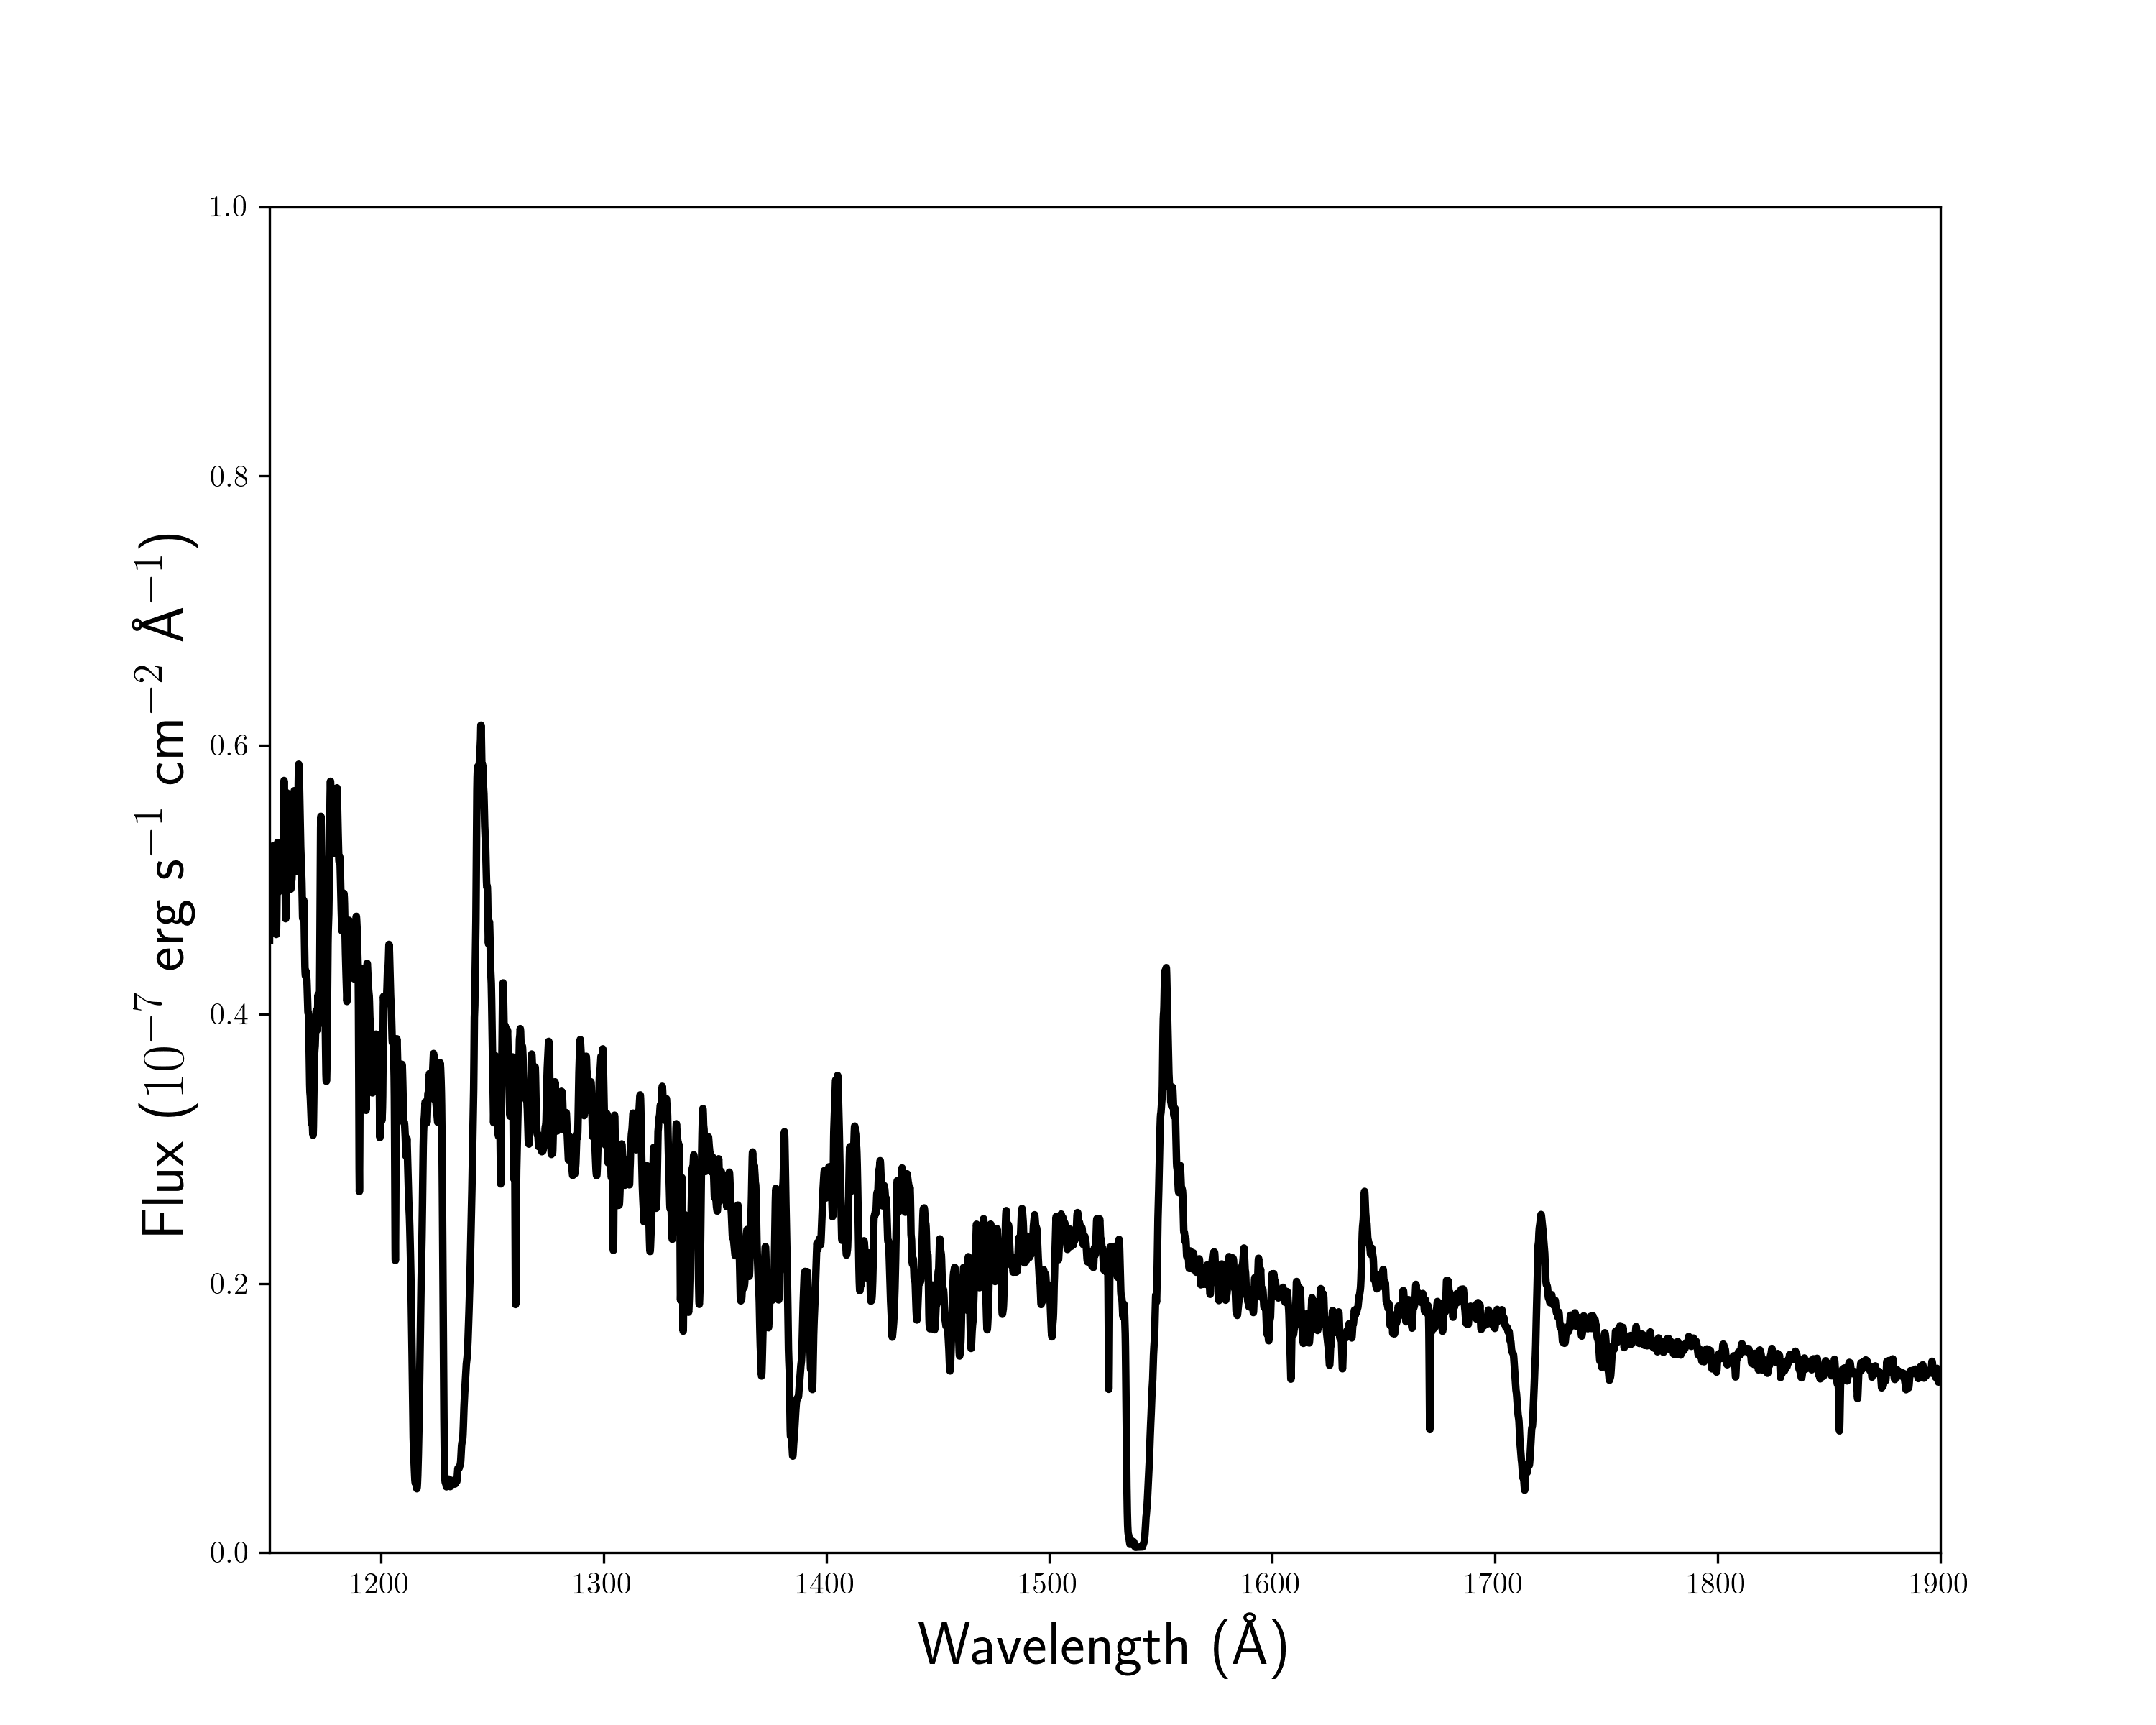
\includegraphics[width=1.0\textwidth]{figures/02-outflows/zeta_pup.png}
\caption
[UV spectrum of one of the O4 supergiant $\zeta$ Puppis.]
{
UV spectrum of one of the brightest massive O stars, 
the O4 supergiant $\zeta$ Puppis. The spectrum is obtained from 
IUE UV observations.
} 
\label{fig:hot_star_wind}
\end{figure}

\subsubsection{Clumping in Stellar Winds}

\label{sec:clumpy_stellar}
\index{clumping}\index{line-driving}\index{hot stars} 
Evidence for clumping in hot star winds comes from a range of sources.
Perhaps the most conclusive is from electron scattering wings
in emission lines: homogenous models overestimate the strength of these
wings, whereas clumpy models produce good agreement with data 
\citep{hillier1984,hillier1991eswingsmodel,hamann1992wr,hamann1994,schmutz1997}.
Further evidence for clumping comes from line variability \citep{prinja1992}
and polarisation \citep{brown1995}. Clumping is theoretically expected
in line-driven winds 
\citep[see section~\ref{sec:line_driving} and the review by][]{owocki2014} 
and is directly dealt with in this thesis.
In chapter 5, I describe the treatment of clumping I have implemented 
in our radiative transfer code, before presenting
results from a clumpy AGN wind model.

\subsection{Outflow Physics}

The spectra in figures~\ref{fig:cordova}, \ref{fig:bals}
and \ref{fig:hot_star_wind} show striking similarities -- 
characteristic broad, P-Cygni-like absorption features in UV resonance
lines extending to high blueward velocities -- 
despite vast differences in mass and scale. 
Furthermore, some of the phenomena observed in e.g. stellar winds may 
naturally solve some of 
the unanswered questions in other systems. For example, clumping
may prevent over-ionization in AGN outflows. It would seem
that at least some of the physics of outflows, like accretion physics,
is universal, and that lessons learned from smaller-scale systems may be
scaleable to AGN and quasars. In order to understand if the similarity extends beyond
a cosmetic one, I will discuss some of the 
underlying physical mechanisms that may be responsible for accelerating
these outflows.\index{outflows} 

\section{Driving Mechanisms}
\index{outflows!driving mechanism} 
Let us consider a parcel of ideal gas. By imposing nothing more than
conservation of mass, energy and momentum on that parcel, and using 
Maxwell's equations, we can write down 
three equations of magnetohydrodynamics (MHD):\index{MHD} 

\begin{equation}
\label{eq:continuity}
\frac{D \rho}{Dt} + \rho \nabla \cdot \vec{v} = 0,
\end{equation}

\begin{equation}
\label{eq:motion}
\rho \frac{Dv}{Dt} = -\nabla P + \frac{1}{4 \pi}(\nabla \times \vec{B}) \times \vec{B} + \rho \vec{g}_{rad} + \rho \vec{g},
\end{equation}

\begin{equation}
\label{eq:energy}
\rho \frac{D}{Dt} \left(\frac{u}{\rho}\right) = P (\nabla \cdot \vec{v}) + \rho \cal{L}.
\end{equation}

Here, $D$ denotes a derivative within the comoving frame of the gas parcel, $\vec{v}$ is the velocity,
$\rho$ is the gas density, $\vec{B}$ is the local magnetic field, 
$\vec{g}_{rad}$ is the radiation
force per unit mass, $\cal{L}$ is the cooling rate of the gas, $u$ is the energy density 
and $\vec{g}$ denotes the gravitational acceleration vector.

Equation~\ref{eq:continuity} is the {\em continuity equation} and describes conservation of mass. 
Equation~\ref{eq:motion} is the {\em equation of motion} and describes conservation of momentum.
Equation~\ref{eq:energy} is the {\em equation of energy conservation}. 
Equation~\ref{eq:motion} can be used to neatly demonstrate how an outflow can be driven. I have 
deliberately written equation~\ref{eq:motion} 
so that all the force terms lie on the RHS. 
For an outflow to be driven from an accreting object, one of the terms on the RHS must
dominate over gravity, $\rho \vec{g}$. These terms thus signify three potential
driving mechanisms.

\begin{itemize}
	\item Magnetic / Lorentz Forces, $\frac{1}{4 \pi}(\nabla \times \vec{B}) \times \vec{B}$.
	\item Radiative Forces, $\rho \vec{g}_{rad}$.
	\item Thermal Pressure, $-\nabla P$.
\end{itemize}

We can now examine under what physical conditions 
(and in which corresponding astrophysical objects)
we might expect these forces to overcome gravity and 
cause a parcel of mass to escape to infinity.
In other words: {\em what might drive a wind?}

\subsection{Thermal Winds}
\index{thermal wind} 
In a disc in hydrostatic equilibrium (HSE),\index{hydrostatic equilibrium} 
thermal pressure balances gravity in the vertical direction. 
The equation of motion in this $z$ direction can then be written as 
\begin{equation}
\label{eq:hse}
\rho \frac{Dv_z}{Dt} = -\frac{\partial P}{\partial z} +  \rho g_z = 0.
\end{equation}
Clearly, if the thermal pressure is significantly 
increased, this equilibrium condition no longer holds. 
This can occur in accretion discs at temperatures in excess of $\sim10^7$~K --
where other forces are negligible compared to thermal pressure -- 
and where the escape velocities are relatively low (i.e. far out in the disc).
Due to the temperature and gravity scalings, this means
that XRBs are natural candidates for showing evidence of thermally driven
winds. The outer disc can be heated to the Compton temperature by 
the central X-ray source,
potentially driving relatively high mass-loss rate outflows 
\citep{begelman1983,woods1996}. 
This driving mechanism has been proposed as a natural explanation
for the ever-present equatorial outflows in soft state XRBs \citep{ponti2012}.
However, they are much less likely candidates in CVs and AGN, because there
the escape velocity tends to greatly exceed the thermal velocity.

\subsection{Radiatively Driven Winds}
\label{sec:rad_winds}
\index{radiation pressure}\index{Eddington limit} 
Under spherical symmetry and for opacities dominated by electron scattering, 
one simply obtains the Eddington limit discussed
in section~\ref{sec:eddington} when $\rho \vec{g}_{rad} = \rho \vec{g}$. 
Hence, sources must be fairly close to the Eddington luminosity in order 
to drive an outflow purely from radiation 
pressure on electrons. There are a number of accreting systems that may drive
super-Eddington (or close to Eddington) outflows, 
such as AGN with UFOs \citep[e.g.][]{reeves2002,pounds2016},
NLSIs \citep{done2015} and ultra-luminous X-ray sources \citep[ULXs;][]{walton2013}.
However, high-state CVs are significantly below the Eddington limit 
\citep{warnerbook}, and at least some BALQSOs have low Eddington fractions 
\citep[$\sim25\%$ have $L/L_{\mathrm{Edd}}<0.1$;][]{grupenousek2015}.
These systems may nevertheless be capable of radiatively driving strong 
outflows due to the influence of line opacity.
% Despite this, line opacity may mean that radiation is still responsible for the 
% powerful outflows in these systems even at $L / L_{Edd} \sim 10^{-3}$.

\subsection{Line-driven Winds}

\label{sec:line_driving}
\index{line driving} 
Under the right ionization conditions, radiation pressure mediated by spectral lines
can be a significant  acceleration term in 
a partially ionized plasma \citep[][hereafter CAK]{CAK75}. 
The most common way to parameterise the cumulative
effect of lines on the radiation force is via the 
{\em CAK force multiplier}, ${\cal M}(t)$,
which modifies the equation for the acceleration due to radiation pressure on electrons
to give \citep[][CAK]{castor1974}\index{force multiplier}
\begin{equation}
\label{eq:force_multiplier}
\vec{g}_{rad} = \frac{\sigma_T F}{\mu c m_p} {\cal M}(t),
\end{equation}
where $F$ is the flux, and $\mu$ is the mean atomic weight.
${\cal M}(t)$ can be approximated by \citep{abbott1982}
\begin{equation}
\label{eq:force_multiplier2}
%% \cal{M}(t) = \sum_{lines} F_C \Delta \nu_D min (1/t, 1/\beta) 
{\cal M}(t) = k~t^{-\alpha} 
\left( \frac{n_e}{10^{11}~{\rm cm}^{-3}}\right)^\delta.
\end{equation}
Here, $k$, $\alpha$ and $\delta$ are parameters\index{O-star}
with best-fit values of 0.28, 0.56 and 0.09, respectively, in O-star winds \citep{abbott1982},
and $v_i$ is the component of the velocity field in the direction
being considered. This is normally a line between the source of radiation and any
given location in the wind.
The dimensionless optical depth, $t$, is given by
\begin{equation}
t = \frac{\sigma_T \rho v_{th}}{m_p | d(v_i) / ds |},
\end{equation}
% and $\beta$ is the ratio of the mass scattering coefficient of the free
% electrons, $\sigma_e$ to the line opacity, $\kappa_L$. $\Delta \nu_D$ is the Doppler
% width.  
where $v_{th}$ is the thermal speed, $\rho$ is the density, and $d(v_i) / ds$ represents
the derivative of $v_i$ along the same direction it has been defined.
It is possible to show \citep[CAK, ][]{owocki1988} that the maximum force multiplier,
${\cal M}_{\mathrm{max}}(t)$,
is around $2000-4000$. This is already an interesting result, as it tells us
that line-driven outflows can be accelerated when accretion rates / luminosities
are much lower than the Eddington limit. Indeed, using 
equation~\ref{eq:force_multiplier} we can see that a radiatively driven wind 
can be accelerated when $L > L_{\mathrm{Edd}} / M(t)$, where $M(t)$ will depend in detail on
the spectral lines in question and their relative ionization and excitation fractions.
Line-driven winds are present in O-stars and Wolf-Rayet stars, and the theory
produces good matches with observations 
\citep[e.g.][]{friend1986,pauldrach1986,pauldrach1994,hamann2008}. 
It is also a strong candidate for driving
the winds seen in high-state CVs when the accretion disc is UV bright 
\citep[][see also section~\ref{sec:proga}]{pereyra1997,proga1998,proga2005}.

\index{BALs}\index{line-locking}
Line driving may be a promising mechanism to explain BAL outflows as well, since
the strong UV resonance lines seen in absorption in O stars are also 
present in BALQSOs. The presence of `line-locked' features \citep{bowler2014} 
and the `ghost of \la' \citep{arav1995, arav1996, north2006}
in the spectra of some BALQSOs also suggests that line-driving is
at least contributing to the acceleration of the wind 
\citep[but see also][]{cottis2010}.
However, the presence of an X-ray source complicates matters.
I have already briefly touched on the `over-ionization' problem
in AGN outflows, but it now has another consequence. Not only will 
strong X-rays prevent the right features forming in the spectrum, but, if
the outflow is line-driven, they may prevent the wind existing in the first 
place. Despite these problems, some hydrodynamic simulations of line-driven AGN winds
have been successful in producing high mass-loss rates (see section~\ref{sec:proga}).

Line-driving is subject to a strong instability known
as the line deshadowing instability 
\citep[LDI;][]{lucysolomon1970,macgregor1979,owockirybicki1984,owockirybicki1985}.
The basic idea is that any velocity perturbation in a line-driven flow can cause a 
`deshadowing' effect, as the fluid element will now
be in resonance with a region of the spectrum that is less absorbed.
Thus, an increase in the line force will occur in proportion
with this velocity perturbation, and the instability can grow. 
Time-dependent numerical modelling of the LDI has shown that it can
produce a clumpy flow \citep{owocki1988,feldmeier1995,surlan2012,owocki2014}
that may explain the observational characteristics of clumping in 
stellar winds (see section~\ref{sec:clumpy_stellar}). 
The LDI is also of interest in CV and AGN winds, as it
may affect the ionization state of the flow and possibly the inferred
mass-loss rates.\index{line-driven instability}\index{clumping} 


\subsection{Magnetic Winds}
\label{sec:mag_winds}
\index{MHD}
There is still great uncertainty over the magnetic fields in accretion discs
and the physics of these magnetic processes. However, the MRI is one of the 
leading candidates for explaining angular momentum transport in accretion discs,
implying that magnetic processes are important in their dynamics. 
Thus, in many senses, magnetic driving is an attractive wind driving mechanism.
There are two main ways in which magnetic forces can drive an 
accretion disc wind, which are best explained by writing down an 
alternative form for the Lorentz force,
\begin{equation}
\vec{F}_m = \frac{1}{4\pi} (\nabla \cdot \vec{B}) \vec{B}  - \nabla \frac{B^2}{8\pi},
\end{equation}
where $B = |\vec{B}|$.
The first term can be thought of as a magnetic {\em tension}
associated with the field lines and the second as an isotropic magnetic
{\em pressure}.\index{magnetic tension}\index{magnetic pressure}\index{MHD}

Historically, the most popular magnetic wind model has been 
the `bead on a wire' mechanism proposed by \cite{blandfordpayne} and 
\cite{pelletier_pudritz}. In these models,\index{MHD wind} 
the poloidal magnetic field is dominant and is anchored in the 
accretion disc. A wind can then be driven by magnetic tension, as the
first term in the above equation operates on fluid elements (`beads') 
on the surface of the accretion disc. This can accelerate
a wind when the poloidal component of the field makes an angle of 
$>30^\circ$ with the normal to the disc surface. These models
are known as magnetocentrifugal winds, as it is the interaction between
centrifugal forces and a strong, large-scale, ordered magnetic field 
threading the disc that drives the wind. 
Magnetocentrifugal wind models have been proposed for both
AGN and YSOs \citep{pelletier_pudritz,konigl1994,kudoh1997},
and numerical simulations have demonstrated that this mechanism can produce
jets and outflows \citep{romanova1997,ouyed1997,ustygova1999}.

In an alternative MHD model the isotropic magnetic pressure 
is responsible for driving the outflow \citep{proga2003a}.
In this case the toroidal component dominates over the poloidal component
and drives a slow, dense outflow which behaves more like a thermally-driven wind 
(i.e. it conserves specific angular momentum rather than angular velocity). 

\section{Accretion Disc Wind Models}
\label{sec:wind_models}

A number of different wind models have appeared in the literature over the 
years, each attempting to explain the different observational characteristics
of quasars and CVs with a mixture of conceptual frameworks and underlying physics.
In AGN and quasars, the authors behind the models attempt to explain the origins of 
BELs and BALs, although some extend their remit into the infra-red, 
radio and X-ray regimes. In CVs, the picture is slightly more straightforward, as 
the geometry of the outflow is better constrained (see section~\ref{sec:cv_winds}).
Below, I will briefly discuss a few examples that have gained traction over the years,
particularly those describing quasars and unification,
before outlining the kinematic prescription I have used in the modelling that forms 
part of this thesis. This prescription has been successfully applied to both CVs 
and AGN.\index{disc wind!model} 

\subsection{MCGV95: A Line-driven Wind Model for AGN}

\begin{figure}
\centering
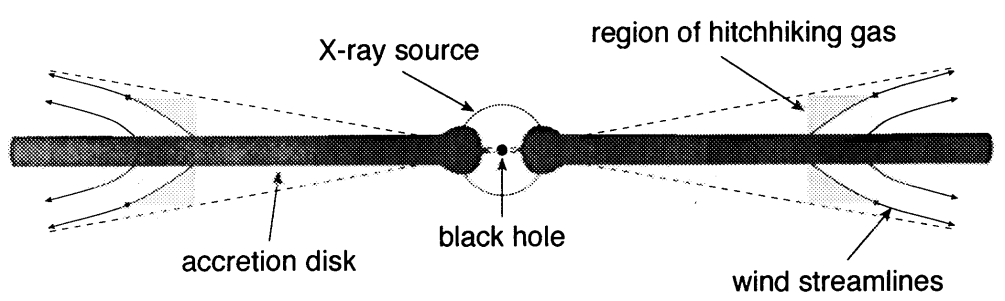
\includegraphics[width=1.0\textwidth]{figures/02-outflows/MCGV95.png}
\caption
[Cartoon showing the geometry of the MCGV95 model.]
{
{\sl Credit: Murray et al. 1995}. 
Cartoon showing the geometry of the MCGV95 model.
} 
\label{fig:MCGV95}
\end{figure}
\index{line driving}\index{shielding}\index{disc wind}  
MCGV95 proposed a model in which a smooth wind rises from an accretion disc with a launch
radius of around $10^{16}$~cm. The wind is equatorial, with an opening angle
of $5^\circ$, and is accelerated by line forces up to a terminal velocity of $0.1c$.
A sketch of the geometry is shown in Fig.~\ref{fig:MCGV95}.
One of the key features of the model is the presence of a `shield' of hitchhiking
gas, which protects the outflow from X-ray over-ionization 
and allows radiation pressure on UV resonance lines to efficiently 
accelerate the flow. 

MCGV95 found that BAL profiles were
seen for an observer looking into the wind cone, and significant collisionally excited
line {\em emission} emerged at low inclinations. This line emission came
from a relatively small BLR ($r_{BLR} \sim10^{16}$~cm) at the base of the wind, 
where densities were high ($n_e \approx 10^{10}$~cm$^{-3}$). 
The MCGV95 model was one of the first successful disc-wind unification models.
It is especially impressive as it includes photoionization calculations and 
quantitative estimates of the resultant line EWs. However, the effects of multiple
scattering and complex radiative transfer effects could not be included 
in the calculations (see chapter 5).

\subsection{De Kool \& Begelman: A Radiatively Driven, Magnetically Confined Wind}

It is, of course, possible that radiation and magnetic fields are both important
in determining the outflow characteristics. In the \cite{dekool1995} model, radiation
pressure drives an outflow from an accretion disc and also compresses the magnetic
field lines that are dragged along with the flow. This causes the magnetic field
strength in certain regions to be comparable to the gas pressure, meaning that clouds
can be magnetically confined in the flow. A diagram is shown in Fig.~\ref{fig:dekool}.
The authors find that such a model would naturally emerge at a fairly equatorial
angle with a covering factor of around $10\%$, and that lower ionization material 
would be intercepted when the system was viewed from higher inclinations, potentially
explaining some of the properties of LoBALQSOs.\index{disc wind}  

\begin{figure}
\centering
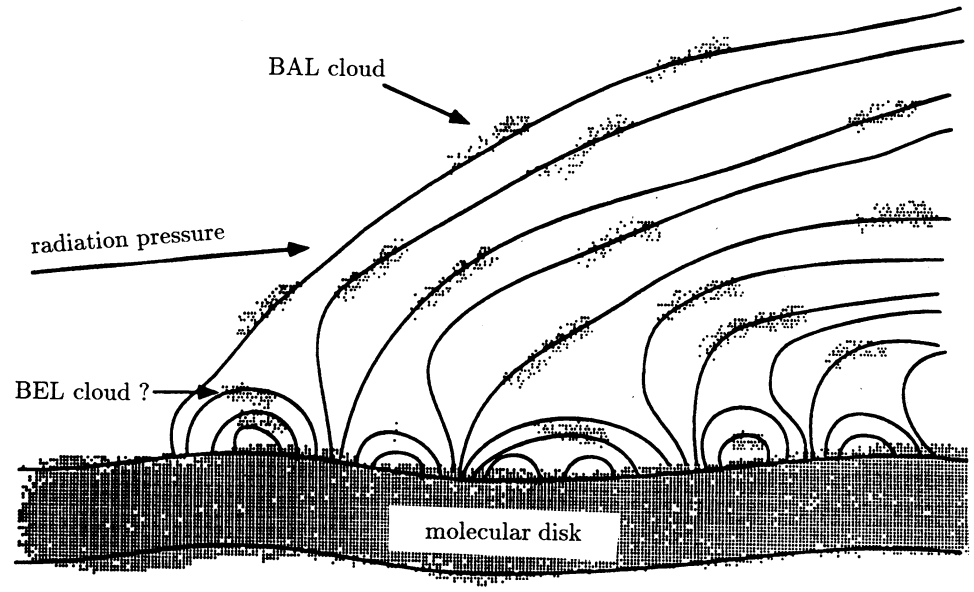
\includegraphics[width=1.0\textwidth]{figures/02-outflows/dekool.png}
\caption
[A cartoon showing the components in the De Kool \& Begelman model.]
{
{\sl Credit: De Kool \& Begelman 1995}. 
A cartoon showing the components in the De Kool \& Begelman model.
} 
\label{fig:dekool}
\end{figure}


\subsection{Elvis 2000: A Structure for Quasars}
\index{AGN!unification}\index{disc wind}  
\cite{elvis2000} expanded on the work of MCGV95 by proposing a simple
disc wind model, empirically designed to explain as much of quasar phenomenology
as possible within one unifying framework. The geometry of Elvis'
is shown in Fig.~\ref{fig:elvis}. As in the two previous models, observers 
looking into the wind cone will see a BALQSO, whereas observers looking down onto
the wind will see a type 1 quasar. Initially, the wind rises vertically, so
that observers looking underneath the flow will see NALs,
due to the small range of velocities intercepted by their line of sight. 

The flow conserves angular momentum, such that the initial Keplerian velocities
determine the BEL widths, before accelerating to BAL-like velocities of $\sim0.1c$.
The wind is assumed to be two-phase, with BEL and BAL clouds embedded in 
a warm, highly ionized medium (WHIM). This WHIM is responsible for WA-like absorption
and the X-ray scattering phenomena seen in AGN. It is also responsible for confining
the BAL and BEL clouds, allowing high densities and cooler temperatures to exist
within the flow. The ionization structure for the wind is stratified, such that the material
further out along the disc plane is somewhat shielded from the inner disc and X-rays.
This allows the lower ionization BEL profiles to form in the right locations,
and also means that LoBAL profiles would be seen at a subset of inclinations.

\begin{figure}
\centering
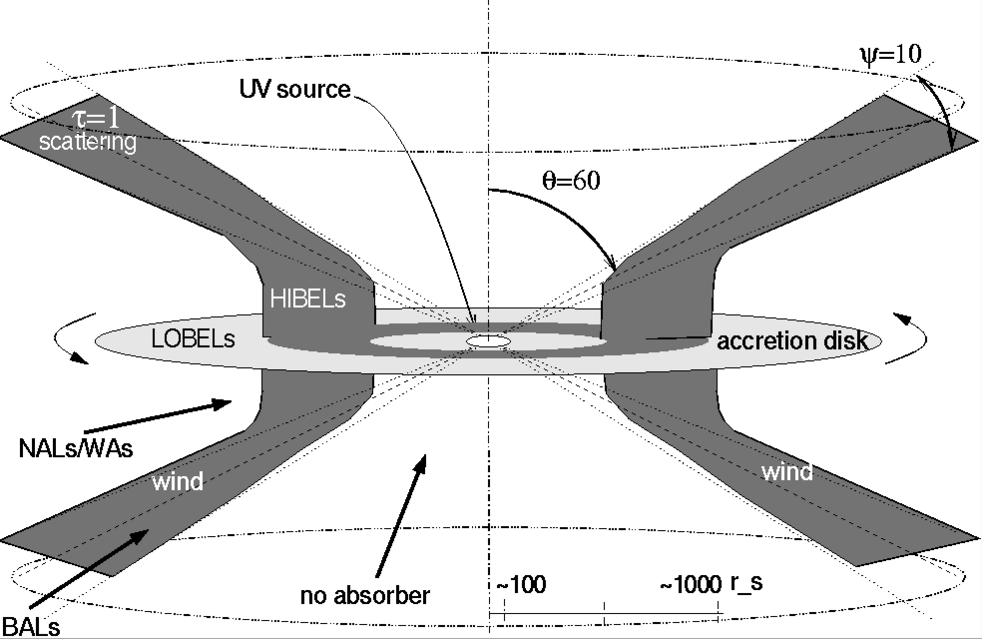
\includegraphics[width=1.0\textwidth]{figures/02-outflows/elvis.png}
\caption
[A schematic showing the main features of the Elvis model.]
{
{\sl Credit: Martin Elvis}. 
A schematic showing the main features of the Elvis model. A biconical
wind rises from an accretion disc, and the observed spectrum is determined 
purely by the viewing angle of the observer.
} 
\label{fig:elvis}
\end{figure}

\subsection{Proga et al.: Line-driven Hydrodynamic Models for AGN and CVs}
\label{sec:proga}
\index{line driving}\index{disc wind} 
Around the turn of the century, Daniel Proga and collaborators 
published a series of important papers in which they conducted 
hydrodynamic simulations of line-driven disc winds in AGN and CVs. 
In the first of these, the problem considered was that of disc
winds in CVs \citep{proga1998}. In their model, the disc was assumed
to radiate according to the $\alpha$-disc model, and the central WD was also included
as a radiating source. They found that when the disc has 
$L / L_{\mathrm{Edd}} \gtrsim 1 / {\cal M}_{\mathrm{max}} (t) \approx 0.001$, 
then strong, line-driven
outflows are driven from a few WD radii with bending angles of $\sim45^\circ$.
This result agreed qualitatively with outflows in CVs, and later efforts to compute
synthetic line profiles produced promising results \citep{proga2002}. This was the
first successful demonstration of line driving in a full hydrodynamic simulation.

The same principle was then applied to the problem of AGN outflows, with the
additional complication of an ionizing X-ray source now included 
\citep[][hereafter PK04]{PSK2000,PK04}. A snapshot from the PK04 model
is shown in Fig.~\ref{fig:PK04}. An inner `failed' wind forms in this simulation,
which initially rises up from the disc before being over-ionized by the central X-rays.
Crucially, this acts as a shield, similarly to the hitchhiking gas proposed by
MCGV95, and allows a line-driven wind to be accelerated further out in the disc. 
This outflow can be seen clearly in Fig.~\ref{fig:PK04}. 

\begin{figure}
\centering
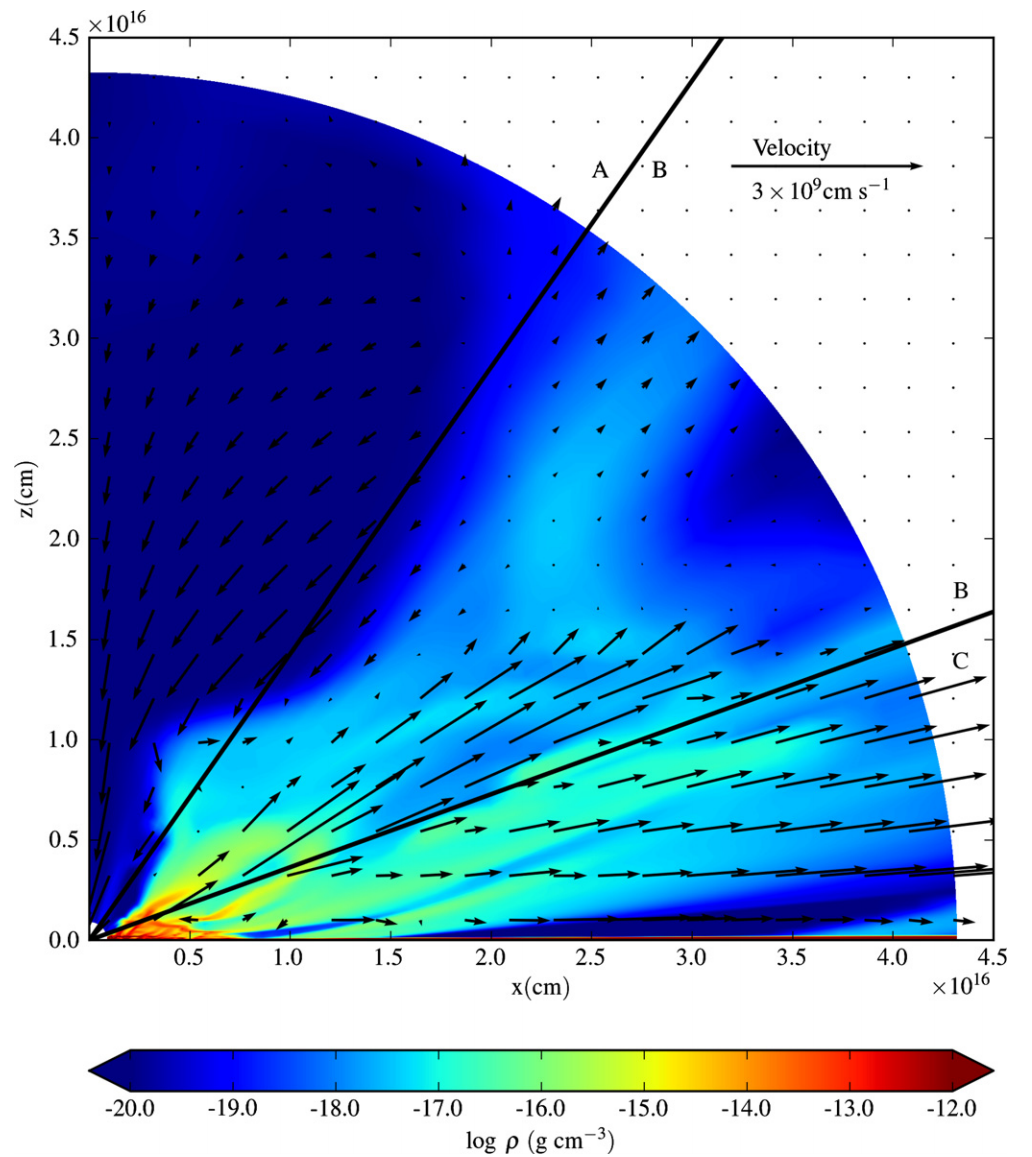
\includegraphics[width=0.8\textwidth]{figures/02-outflows/pk04_h14.png}
\caption
[Density snapshot of the PK04 model.]
{
{\sl Credit: Higginbottom et al. 2014.}. 
A snapshot of the PK04 model. Colours shows the density and 
arrows show the velocity of the flow. 
The radial lines separate three areas described by H14.
} 
\label{fig:PK04}
\end{figure}

One of the interesting results of these  simulations is that they tended
to produce somewhat unsteady, clumpy flows. In the CV case, this was caused by
the interaction between the line force and gravity, as both force terms vary 
differently with height. In the AGN case, it was instead due to the critical
importance of the ionization state on the line force. Parcels of gas can only 
be accelerated if they have the `right' ionization state, and this depends
critically on both their density and the radiation field they see. This causes
a coupling between the dynamics of the flow and the path of ionizing radiation. 
The radiation field also helps
determine the geometry of the outflow, as increasing the strength of the radiation
interior to the launch radius tends to flatten out the wind and lead to more
equatorial outflows \citep{proga1998,proga2005}. Indeed, the outflow 
in the CV case is more collimated than the equatorial AGN outflow for this reason.
This is particularly important when considering quasar unification, as it means
the viewing angles of BALQSOs can provide information about where the wind is launched.
Along with more empirical motivations, the results of this hydrodynamical modelling
are one of the reasons for adopting different geometries for the CV and quasar 
models presented in chapters 4 and 5 respectively.

It is worth noting that the smaller scale LDI could not be included in this model,
partly for computational reasons and partly because of the approximations 
used to treat the radiation field. Treating the radiation transport is also
important for other reasons. 
\citet[][hereafter H14]{H14} showed that, in this particular geometry, 
multiple scattering actually makes shielding
ineffective, and radiation will simply find its way around the failed wind
to over-ionize the flow beyond \citep[see also][]{sim2010_hydro}.
Ideally, full radiative transfer and hydrodynamical simulations would be used
to estimate the viability of line-driven winds. Our team is currently working 
on this problem (see H14 for the first step); however, much 
can also be learned from simpler, kinematic prescriptions for outflows, which can
already be modelled with full treatments of radiative transfer and ionization.  

\section{A Kinematic Prescription for a Biconical Wind}
\label{sec:sv93_model}

\citet[][hereafter SV93]{SV93}\index{disc wind}  
expanded on the work of the stellar wind community \citep[e.g.][]{AL85} 
in proposing a kinematic model for an accretion disc wind. Unlike 
hydrodynamical models, this model has no real predictive power in terms of velocities
and mass-loss rates. Instead, one sets these quantities in advance and examines the 
resultant properties of the flow and the emergent spectra. The SV93 prescription
is the most common way of describing the outflow in the 
radiative transfer code \py\ (see chapter 3)
and has been used to simulate spectra for CVs \citep[][chapter 4]{LK02, M15}, 
AM CVn systems \citep{kusterer2014} and AGN/quasars 
\citep[][chapter 5]{higginbottom2013, M16, yong2016}. 
An alternative description was developed by \cite{KWD95} and has been used
in similar applications \citep{LK02, simlong2008, sim2010}, as 
well as for young-stellar objects \citep[YSOs;][]{simmacro2005}.
Kinematic prescriptions have thus been a useful tool in allowing quantitative
tests of conceptual models, specifically for assessing their ability to reproduce
the observed spectra of a variety of astrophysical systems.

In the SV93 parametrization,
a smooth, biconical disc wind emanates from the accretion disc between 
$r_{\mathrm{\mathrm{min}}}$ and $r_{\mathrm{\mathrm{max}}}$. A schematic is shown in Fig.~\ref{fig:sv93}.
The covering fraction of the outflow is 
also controlled by the inner and outer opening angles of the wind, $\theta_{\mathrm{min}}$ and
$\theta_{\mathrm{max}}$, and the launch angle of the other streamlines is given by 
\begin{equation}
\theta(r_0) = \theta_{\mathrm{min}} + (\theta_{\mathrm{max}} - \theta_{\mathrm{min}}) \left(\frac{r_0 - r_{\mathrm{min}}}{r_{\mathrm{max}} - r_{\mathrm{max}}} \right)^{\gamma},
\label{eq:wind_theta}
\end{equation}
where $r_0$ is the launch radius of the streamline.

\begin{figure}
\centering
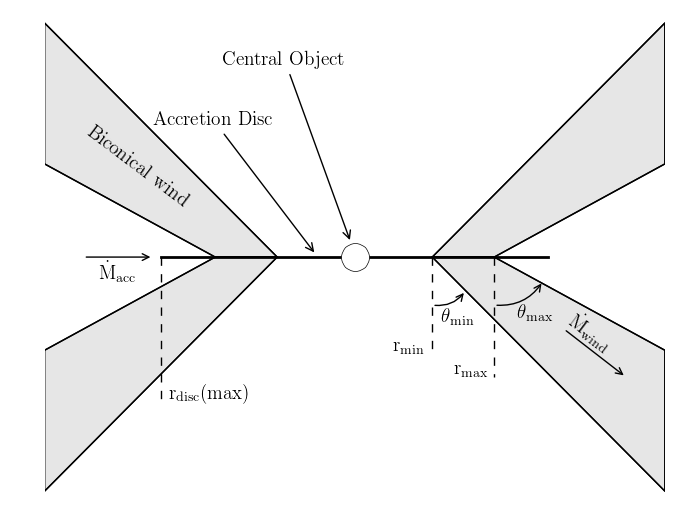
\includegraphics[width=1.0\textwidth]{figures/02-outflows/cartoon_general.png}
\caption
[A schematic showing the geometry and kinematics of the SV93 model]
{
A schematic showing the geometry and kinematics of the SV93 model. 
} 
\label{fig:sv93}
\end{figure}

The poloidal (non-rotational) velocity field of the wind, $v_l$, is given by
\begin{equation}
v_l=v_0+\left[v_{\infty}(r_0)-v_0\right]\frac{\left(l/R_v\right)^{\alpha}}{\left(l/R_v\right)^{\alpha}+1},
\label{eq:v_law}
\end{equation}
where $l$ is the poloidal distance along a particular wind
streamline. The terminal velocity along a streamline, $v_{\infty}$, is
set to a fixed multiple of $v_{\mathrm{esc}}$, the escape velocity at the launch
point. The terminal velocity will therefore be higher for streamlines closer
to the inner disc edge.
The launch velocity from the disc surface, $v_0$, is assumed to
be constant (set to $6$~km~s$^{-1}$). Once the wind is launched, it
accelerates, reaching half of its terminal velocity at $l = R_v$. The
velocity law exponent, $\alpha$, controls how quickly the wind
accelerates. Larger values of $\alpha$ cause the main region of 
acceleration to occur close to $R_v$, whereas smaller values
correspond to fast acceleration close to the disc (see
Fig.~\ref{acc_law}). The rotational velocity, $v_\phi$, is 
Keplerian at the base of the streamline, 
and the wind conserves specific angular momentum, such that
\begin{equation}
v_\phi r = v_{k} r_0,
\label{eq:vrot}
\end{equation}
where $v_{k}=(GM_{WD}/r_0)^{1/2}$.
The mass-loss rate per unit surface area, $\dot{m}^\prime$,
can be controlled by a free parameter, $\lambda_m$, such that
\begin{equation}
\dot{m}^\prime \propto \dot{M}_W~r_0^{\lambda_m} \cos [\theta(r_0)],
\label{eq:dmda}
\end{equation}
where $\dot{M}_W$ is the total mass loss rate in the wind. This equation is normalised so 
that when integrated over both sides of the disc the correct $\dot{M}_W$ emerges.
I have adopted $\lambda=0$ throughout this thesis, which corresponds to uniform
mass loss across the disc. This could have an effect on the level of shielding present 
in the flow, and the location of the emission line regions, but should not affect the qualitative
conclusions; this is briefly discussed in section~\ref{sec:param_sens}.
The density at a given point can then be calculated by imposing mass conservation
and using the velocity law. At the base of the wind, the density is 
given by
\begin{equation}
\rho (r_0) = \frac{\dot{m}^\prime(r_0)}{v_z(r_0}.
\label{eq:rho0}
\end{equation}
At a coordinate $(r,z)$ in the wind, the density is then
\begin{equation}
\rho (r, z) = \frac{r_0}{r} \frac{d r_0}{dr}\frac{\dot{m}^\prime(r_0)}{v_z(r,z)},
\label{eq:rho_rz}
\end{equation}
where the corresponding $r_0$ is found by considering the streamline that 
passes through $(r,z)$. These equations govern the kinematics
and densities in the wind in the SV93 prescription, which is used
extensively throughout this thesis. 
% This prescription is used to describe the outflow in
% the radiative transfer code \py. 
% The radiative transfer procedure and 
% ionization calculation is described in chapter 3, and specific
% applications of this model are described in
% chapters 4 and 5.


\begin{figure}
\centering
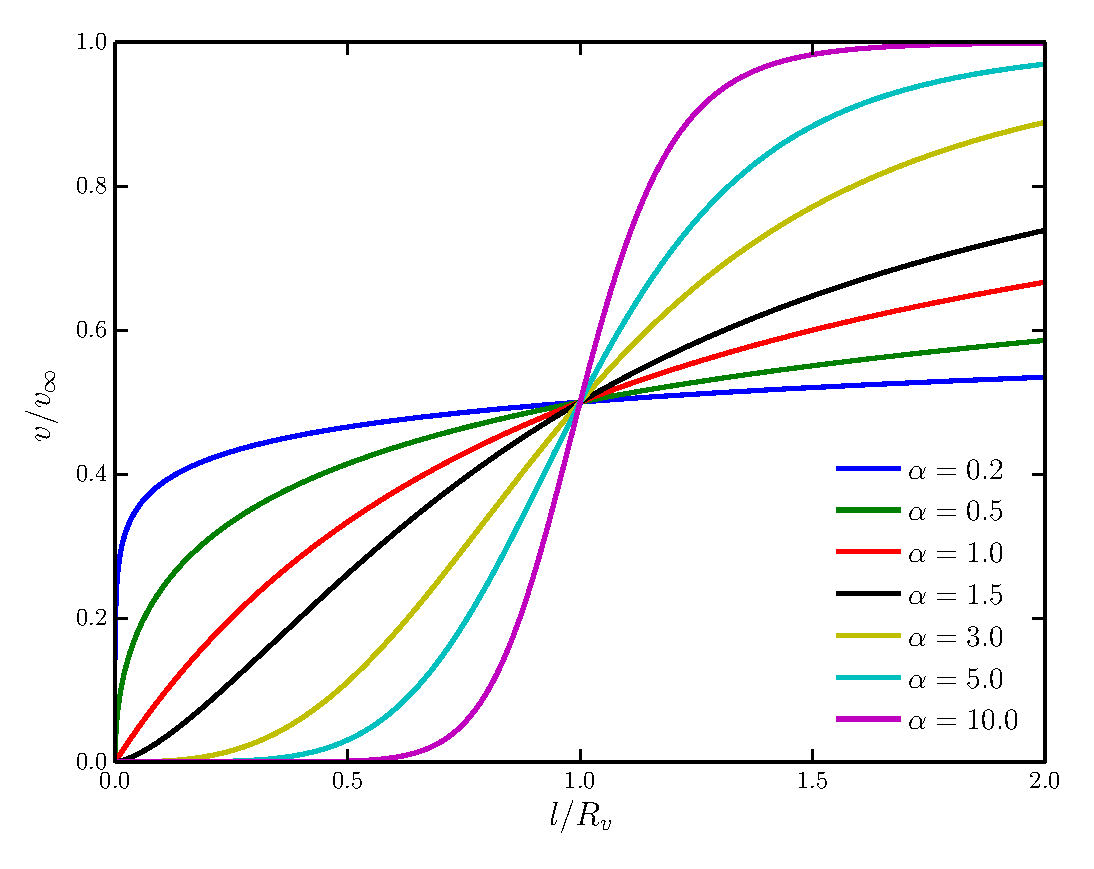
\includegraphics[width=1.0\textwidth]{figures/05-cvpaper/acc_law.eps}
\caption
[The SV93 velocity law for various values of the
acceleration exponent, $\alpha$.]
{
The SV93 velocity law for various values of the
acceleration exponent, $\alpha$.
%%{\bf JM: KSL has suggested we ditch this}
} 
\label{acc_law}
\end{figure}




\section{The big picture: AGN Feedback}
\label{sec:agn_feedback}
\index{AGN!feedback} 
The event horizon of a $10^9~M_\odot$ BH is approximately 
$10^{15}$~cm, a billionth of the radius of a typical galactic bulge. This is 
roughly the ratio in size between a small coin and the 
Earth. Even the sphere of gravitational influence of the BH is roughly 
$1000$ times smaller than the size of the galactic bulge.
Despite this vast different in scale, there is strong evidence
that the physics on the scale of the gravitational
radius of the BH affects the evolution and dynamics of its host galaxy.
This becomes less surprising when considering the {\em energetics} of accretion.
The binding energy of a galactic bulge, with mass 
$M_{\mathrm{bulge}}$ and velocity dispersion $\sigma_*$, is 
\begin{equation}
E_{\mathrm{bulge}} \approx M_{\mathrm{bulge}} \sigma_*^2,
\end{equation} 
while the energy released in growing a black hole to a 
mass $M_{BH}^\prime$ is (equation~\ref{eq:restmass}, assuming $\eta=0.1$)
\begin{equation}
E_{BH} \approx 0.1 M_{BH}^\prime c^2.  
\end{equation}
By combining these two equations, and substituting in typical numbers 
($\sigma_* = 0.001c$, $M_{BH}^\prime / M_{\mathrm{bulge}} = 10^{-3}$), we can show that 
\begin{equation}
\frac{E_{BH}}{E_{\mathrm{bulge}}} \approx 10^{-4} \left( \frac{c}{\sigma_*} \right)^2 \sim 10.
\end{equation}
In other words, the energy released when growing a BH can significantly exceed
the binding energy of the galactic bulge. This energetic 
argument is, of course, not sufficient to claim that the accreting BH must affect its
host. For example, if the radiated energy never experienced an 
optical depth of $\sim 1$, it could not couple to the galactic bulge. However,
we have already seen that many outflows in AGN possess kinetic luminosities that
are significant compared to the bolometric luminosity. Thus, outflows 
(and jets) may provide a mechanism by which the vast accretion energies can
be transferred to the BH environment.

\subsection{Observational evidence for feedback}
\index{$M_{BH}-\sigma_*$ relation}\index{$M_{BH}-M_{\mathrm{bulge}}$ relation}
Perhaps the most famous pieces of evidence for some kind of long-distance 
relationship between a central BH and its host galaxy are the 
$M_{BH}-\sigma_*$ \citep{ferrarese2000,gebhardt2000,gultekin2009} and $M_{BH}-M_{\mathrm{bulge}}$ 
\citep{magorrian1998,haring2004,mcconnell2013} correlations, 
shown in Fig.~\ref{fig:msigma} and Fig.~\ref{fig:mbulge}, respectively.
By themselves, these correlations would not necessarily imply
that the AGN is having an impact on its environment. Indeed, there are many different
theoretical models for the origin of these relations 
\citep[e.g][]{somerville2001,adams2001,burkert2001,king2003,croton2006,kormendy2013}. 
However, there are many other clues that outflows and jets from AGN can affect
the host galaxy evolution and morphology.

\begin{figure}
\centering
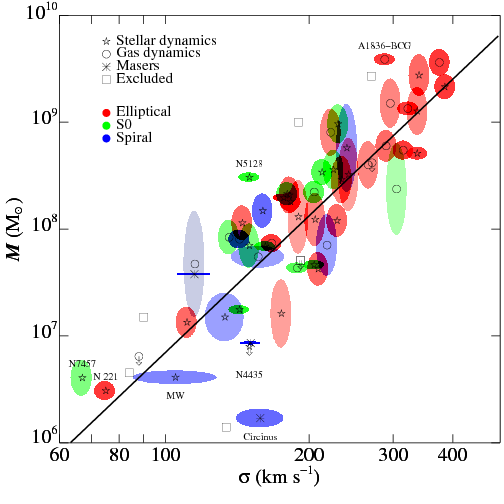
\includegraphics[width=0.7\textwidth]{figures/02-outflows/msigma.png}
\caption
[The $M_{BH}-\sigma_*$ correlation.]
{
{\sl Credit: Gultekin et al. 2009}. 
The $M_{BH}-\sigma_*$ correlation.
} 
\label{fig:msigma}
\end{figure}

\begin{figure}
\centering
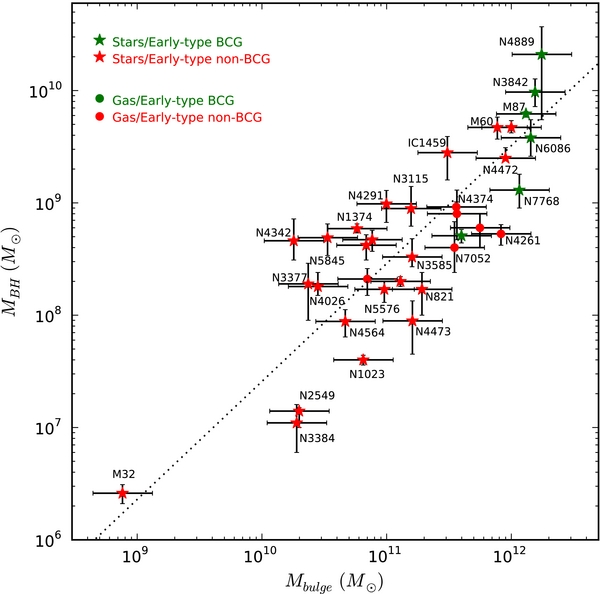
\includegraphics[width=0.7\textwidth]{figures/02-outflows/mbulge.jpg}
\caption
[The $M_{BH}-M_{bulge}$ correlation.]
{
{\sl Credit: McConell \& Ma 2013}. 
The $M_{BH}-M_{bulge}$ correlation.
} 
\label{fig:mbulge}
\end{figure}

The galaxy luminosity function describes\index{galaxy luminosity function}
the number of galaxies as a function of luminosity and is generally modelled
with the \cite{schechter1976} function. Theories of 
galaxy evolution tend to overpredict the number of galaxies at the
high luminosity end, which can be avoided by invoking quenching
of star formation by the central AGN \citep[e.g.][]{read2005,bongiorno2016}.
Galaxies also show bimodality in their colour distributions 
\citep{strateva2001,bell2003a,baldry2004}, 
with a clear separation between a blue, star-forming
main sequence, and a red sequence with lower 
specific star formation rate (sSFR). Furthermore, these two 
sequences tend to lie in the same regions of colour space as the 
host galaxies of high and low \index{galaxy colour distribution}
Eddington fraction AGN, respectively, implying that the AGN may be 
directly responsible for quenching star formation and moving 
a galaxy onto the `red and dead' branch. This has been demonstrated in 
several numerical simulations \citep[e.g.][]{springel2005,croton2006}.

There is also evidence that AGN are energetically 
significant on scales larger than the galactic bulge. X-ray observations
of cool core clusters and elliptical galaxies
can show dramatic X-ray cavities or bubbles\index{X-ray cavity}
up to 50~kpc across, with a radio-loud AGN at the centre
\citep[Fig.~\ref{fig:xray_bubbles}]{randall2011,cavagnolo2011,fabian2012}. This
shows how radio jets can significantly impact the surrounding gas,
a flavour of feedback known as `radio' or `kinetic' mode.
These cavities also provide an estimate of the kinetic power of a radio
jet, as the volume of the bubble and surrounding gas pressure gives a 
rough estimate of the $PV$ work done by the jet. This can be divided by
an age estimate for the cavity, giving powers
of up to $10^{46}$~erg~s$^{-1}$, which are weakly 
correlated with the radio luminosity of the source 
and can be large even for modest radio power \citep{birzan2008}. 

% \begin{figure}
% \centering
% 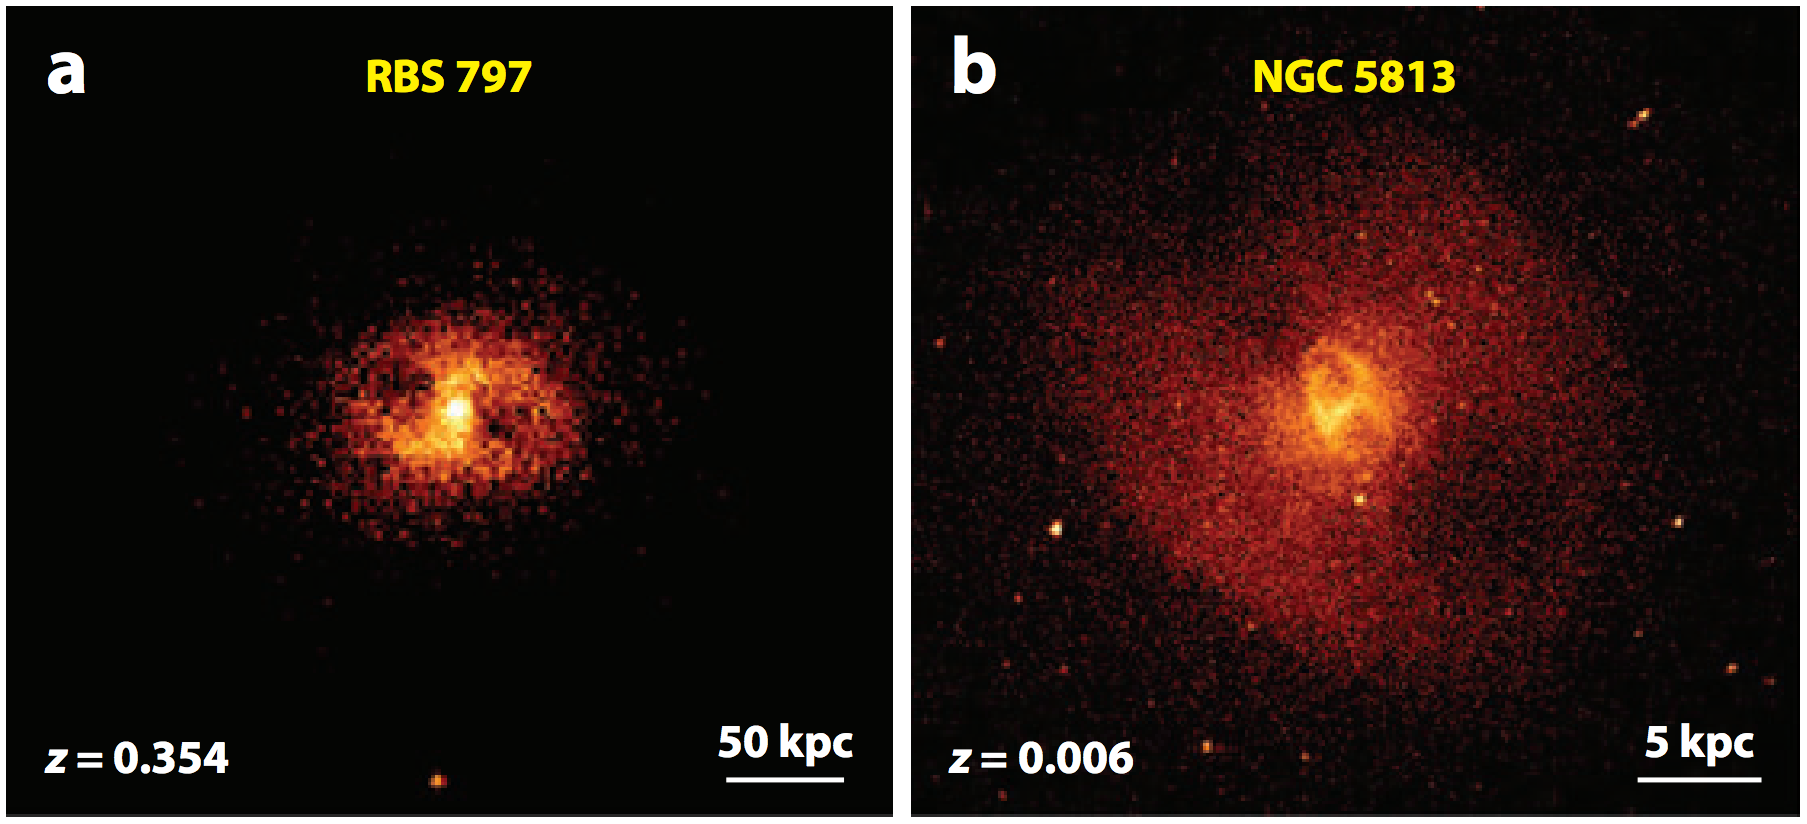
\includegraphics[width=1.0\textwidth]{figures/02-outflows/xray_cavities.png}
% \caption
% [{\sl Chandra} X-ray images showing two examples of X-ray cavities.]
% {
% {\sl Figure adapted from Fabian 2012}. 
% {\sl Chandra} X-ray images showing two examples of X-ray cavities,
% illustrating how a radio jet from an AGN can have a dramatic impact 
% on its environment. a) The RBS 797 Cluster (Cavagnolo et al. 2011). 
% b) elliptical galaxy NGC 5813 (Randall et al. 2011).
% } 
% \label{fig:xray_bubbles}
% \end{figure}

However, jets are not the only way for AGN to interact with 
their environment. I have already briefly discussed in section~\ref{sec:ufos}
how fast AGN winds can drive larger-scale molecular outflows.
This can be seen spectacularly in the FeLoBALQSO Mrk231,\index{Mrk 231}
where integrated field spectroscopy shows kiloparsec-scale
neutral gas outflows \citep{rupke2011}.
Furthermore, \cite{king2003} expanded on the ideas of \cite{silkrees1998} and
considered a super-Eddington, momentum-driven outflow expanding into the surrounding gas. 
This model naturally reproduces the observed slope of the $M_{BH}-\sigma_*$
relation. This line of argument was used to suggest that super-Eddington accretion must be
common near the end of a quasar cycle, although it is worth noting that line-driving,
or non-radiative driving, means that super-Eddington accretion rates are 
not necessarily required to drive such an outflow. Intriguingly, it follows that 
understanding outflow physics has implications for understanding 
the accretion history of BHs.\index{outflows!momentum-driven}

% \begin{figure}
% \centering
% 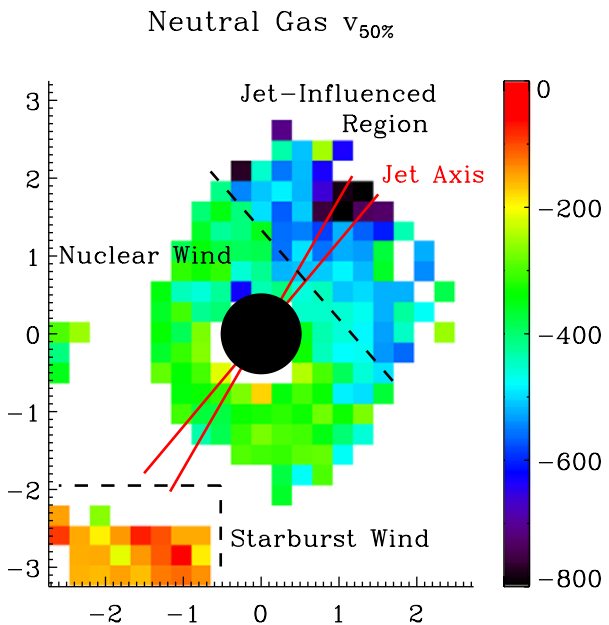
\includegraphics[width=0.8\textwidth]{figures/02-outflows/rupke2.png}
% \caption
% [Results of Gaussian line profile fitting to 
% integral field spectroscopy of Mrk 231.]
% {
% {\sl Credit: Rupke \& Veilleux 2011}. 
% Results of Gaussian line profile fitting to 
% integral field spectroscopy of Mrk 231. The quantity
% shown, $v_{50\%}$, corresponds to the centre of the fitted Gaussian
% profile and indicates that high outflow velocities 
% are present in the neutral gas.
% } 
% \label{fig:rupke}
% \end{figure}


\subsection{Alternative Explanations}

It cannot yet be proven that AGN are the drivers of the observed 
galaxy colour evolution, high-end luminosity function discrepancy or
BH-bulge correlations. 
In particular, it is also possible that mergers are responsible for these phenomena. 
For example, major galaxy mergers may explain the `red and dead' branch
of the galaxy colour bimodality \citep[e.g.][]{somerville2001,baldry2004}. 
However, AGN winds and jets are clearly 
energetically significant with respect to their host galaxies, so estimating
their kinetic powers accurately is important in discriminating between in-situ
and ex-situ scenarios. 

Having established the astrophysical importance of outflows, 
I will now move on to discussing how we might go about 
accurately modelling the ionization states of accretion disc winds 
and their emergent spectra.


 % Experimental Setup

\newpage
\lhead{\emph{3. MCRT and Ionization}}  % Set the left side page header to "Contents"
\chapter{Monte Carlo Radiative Transfer and Ionization}

\epigraph{``I'm splashing greys where once was glowing white''}{{\sl Mike Vennart, Silent/Transparent}}

In the previous chapters I have given an introduction to the field and 
some relevant background relating to accretion 
discs and their associated outflows. Now it proves useful
to discuss the specific {\em methods} I will use
in order to answer some of the questions raised so far.
In particular, I will discuss radiative transfer and photoionization
techniques.

{\sl Notation: This section contains a lot of algebraic quantities and sums over
ions, levels, and so on. Throughout, I use $N$ to denote fractional
populations of ions and $n$ to denote fractional populations of levels. 
The primed quantities $\ellp$ and $\up$ follow the convention of 
\cite{lucy2002} in that they denote sums over all lower/upper levels.
The symbol ${\cal R}$ denotes a total rate (radiative + collisional), 
and the symbol $C$ is a collisional rate, whereas ${\cal C}$ is a cooling 
rate. Starred quantities are evaluated at the stated temperature but 
in local thermodynamic equilibrium, following \cite{mihalas}. An $S$ 
superscript denotes that the estimator pertains to simple-atoms.
}
\index{Monte Carlo radiative transfer}


\section{Fundamentals of Radiative Transfer}
\index{radiative transfer}
\begin{figure}
\centering
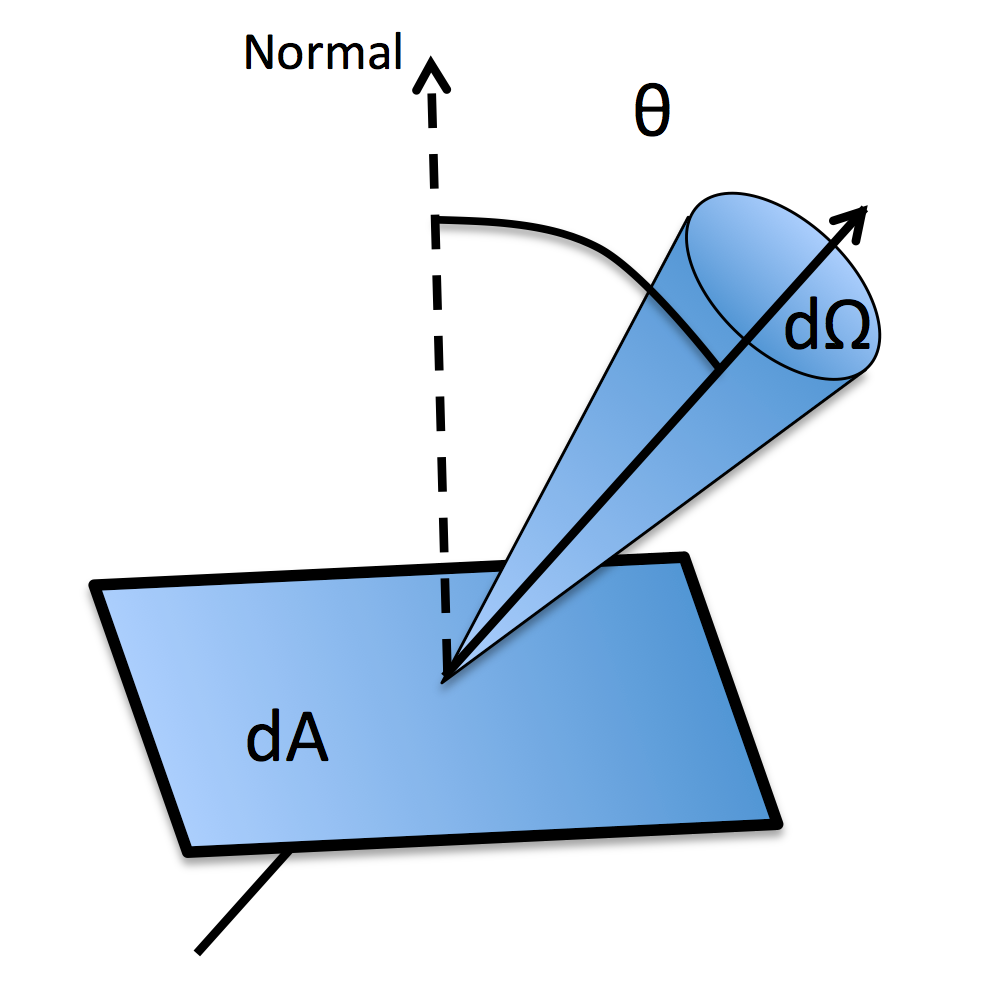
\includegraphics[width=0.5\textwidth]{figures/03-radtrans/rays_schematic.png}
\caption
{
A schematic showing a ray obliquely incident on a surface of area $dA$.
The labeled quantities are used in the definition of specific intensity.
} 
\label{fig:ray}
\end{figure}

Let us consider a ray passing through a reference surface $dA$ and 
making an angle $\theta$ with the normal to this surface. The energy
flow can then be related to the
{\em specific intensity}, $I_\nu$, by
\index{radiative transfer}\index{specific intensity}
\begin{equation}
I_\nu = \frac{dE}{d\Omega~dt~dA~d\nu},
\end{equation}
which has units of ${\rm erg~s^{-1}~Hz^{-1}~sr^{-1}~cm^{-2}}$. The specific
intensity is the most fundamental quantity of radiative transfer as it describes 
everything about the radiation field: its time, angular, spatial and frequency
dependence.
By successively multiplying by $\cos \theta$ and integrating over solid angle we 
can obtain the first and second `moments' of the radiation field. These
are the flux, $F_\nu$ and momentum flux, $p_\nu$, respectively, given by\index{momentum flux}
\begin{equation}
F_\nu = \int I_\nu \cos \theta~d \Omega,
\end{equation}
\begin{equation}
p_\nu = \frac{1}{c} \int I_\nu \cos^2 \theta~d \Omega.
\end{equation}
The {\em mean intensity}, $J_\nu$, is
\begin{equation}
J_\nu = \frac{1}{4 \pi} \int I_\nu~d \Omega.
\end{equation}
The mean intensity is particularly\index{mean intensity}
useful when one wants to ignore the solid angle dependence of the radiation,
for example when considering the impact of an ionizing radiation field.

The equation describing the specific intensity change along a path element $ds$
is the radiative transfer equation,\index{radiative transfer!equation of} 
\begin{equation}
\frac{d I_\nu}{ds} = -\kappa_\nu I_\nu + j_\nu, 
\label{eq:rte}
\end{equation}
where $\kappa_\nu$ and $j_\nu$ are the absorption and emission coefficients, respectively.
If we define the optical depth, $d \tau_\nu = \kappa_\nu ds$, this can be recast as
\begin{equation}
\frac{d I_\nu}{d \tau_\nu} = -I_\nu + S_\nu,
\label{eq:formal_rte}
\end{equation}
where $S_\nu=j_\nu/\kappa_\nu$ is the source function. This equation\index{source function}
can be solved to give the {\em formal solution to the radiative transfer equation},
\begin{equation}
I_\nu = I_{\nu,0}~e^{-\tau_\nu} + \int^{\tau_\nu}_0 S_\nu (\tau^\prime_\nu)~e^{\tau^\prime_\nu-\tau_\nu} d \tau^\prime_\nu.
\label{eq:rte_solution}
\end{equation}
A useful limit is when the source function is constant in the absorbing medium, in which case
the integral can be easily evaluated to give
\begin{equation}
I_\nu = I_{\nu,0}~e^{-\tau_\nu} + S_\nu (1 - e^{-\tau_\nu}).
\label{eq:rte_solution}
\end{equation}

% The mean intensity, $J_\nu$ is a particularly useful quantity when calculation the ionization
% state 



\subsection{Spectral Line Formation}

\index{emission line}\index{line formation}\index{absorption line}
From the above equations, it is trivial to show how emission and absorption lines form when
the source function is approximately constant.
Say we have a plasma illuminated by a blackbody of temperature $T_0$, such that
$I_{\nu,0} = B_\nu (T_0)$. The plasma layer then has a different temperature, $T$,
such that $S_\nu = B_\nu (T)$ in that medium. By inspecting equation~\ref{eq:rte_solution}
we can see that if we are optically thick within the line, but optically
thin in the continuum, then inside the line the source term is dominant and outside 
the line the first $I_{\nu,0}~e^{-\tau_\nu}$ term dominates. Therefore, if $T > T_0$ we will 
see an emission line, and if $T < T_0$ we will see an absorption line. 
% This approach describes line emission in the blackbody limit; for more complicated SED shapes
% it is necessary to construct simple model atoms.

\subsection{Local Thermodynamic Equilibrium}
\label{sec:lte}


An important physical limit is that of local thermodynamic equilibrium (LTE).
\index{LTE}\index{blackbody}
This is a first-order way to describe the physical conditions of a plasma and assumes
that all the properties of the plasma, such as the level populations and source function,
are the same as those in thermodynamic equilibrium for local values of 
temperature and density. For this to be the case, the principle of 
{\em detailed balance} must also apply, in which every\index{detailed balance} 
process by which electrons transition between states must be exactly 
balanced by its inverse process. In LTE, the electron temperature, 
$T_e$, is equal to the temperature of the radiation field, $T_R$, and
the source function is given by a blackbody, i.e. $S_\nu = B_\nu (T_R)$.
Three microscopic requirements of LTE also follow \citep{mihalas}:

a) The velocities of the electrons and ions in the plasma obey Maxwellian
distributions, such that
\begin{equation}
f(v) = 4 \pi \left( \frac{m_e}{2 \pi kT_e} \right)^{3/2} v^2 
\exp \left( - \frac{m_ev^2}{2kT_e} \right),
\label{eq:maxwellian}
\end{equation}
where $m_e$ is the mass of an electron.\index{Maxwellian distribution}

\smallskip

b) The ionization state of the plasma is governed by the {\em Saha equation},
which states that two adjacent ions have relative populations given by
\begin{equation}
\frac{N_{i+1}n_e}{N_i} = \frac{2g_{i+1}}{g_i} 
\left( \frac{2 \pi m_e kT_e}{h^2} \right)^{3/2}
\exp(-h \nu_0/kT),
\label{eq:saha}
\end{equation}
where $g_i$ is the multiplicity of ion $i$ and $\nu_0$ is the threshold frequency.
\index{Saha equation}

\smallskip

c) The excitation state of the plasma is governed by {\em Boltzmann statistics}.
A level $j$ then has a population relative to ground governed by
\begin{equation}
\frac{n_{j}}{n_1} = \frac{g_j}{g_1} \exp(-E_j/kT_e), 
\label{eq:boltzmann}
\end{equation}
where $E_j$ is the energy difference between the two levels and 
$g_j$ is the statistical weight of level $j$.\index{Boltzmann statistics}

\smallskip

Although these three assumptions are sometimes valid, in many astrophysical situations
there can be large departures from LTE. A good example of these departures is when
the SED is not a blackbody and is affected by absorption -- 
as is the case in AGN and other accreting systems. The Maxwellian assumption 
is probably the most reliable, but even this may break down
when high-energy photons create suprathermal electron distributions 
\citep{humphrey2014}.\index{LTE}\index{suprathermal electron distribution}.

\subsubsection{Dilute Approximation}
\label{sec:dilute}
A first step away from LTE is to introduce the dilute approximation. In this case,
we relax the assumption that $T_R = T_e$ and assume that the mean intensity is given
by a dilute blackbody, i.e.\index{dilute approximation}\index{LTE}  
\begin{equation}
J_\nu = W B_\nu (T_R),
\label{eq:dilute_jnu}
\end{equation}
where $W$ is the dilution factor. The ionization state can then be approximated 
with a modified Saha equation \citep{AL85,ML93},\index{ionization state} 
\begin{equation}
\frac{N_{i+1} n_e}{N_i} = W [\xi + W(1-\xi)]
\left(\frac{T_e}{T_R}\right)^{1/2}
\left(\frac{N_{i+1}n_e}{N_i}\right)^*_{T_R}, \label{eq:ml93}
\end{equation}
where $\xi$ is the fraction of recombinations that go directly to
the ground state.\index{recombination}
The excitation state can also be approximated (fairly poorly) 
with a dilute Boltzmann equation \citep{AL85,lucy1999sne}
\begin{equation}
\frac{n_{j}}{n_{1}} = W \frac{g_j}{g_{1}} \exp(-E_j/kT_R).
\label{eq:dilute_boltzmann}
\end{equation}


\subsection{The Two Level Atom}
\index{two level atom}
The two level atom formalism is well described by \cite{mihalas}.
Let us consider an atomic model consisting of two levels that are linked 
by radiative and collisional transitions. 
Whilst this model is clearly a simplification, it nonetheless allows
for a first step into non-LTE line transfer and proves useful for modelling
the resonance lines briefly touched on in chapter 2.\index{line transfer}

To construct our simple model a few assumptions are necessary. The first
is the assumption of {\em statistical equilibrium}. This is the principle \index{statistical equilibrium}
that the total rate into a given atomic level/state is equal to the 
total rate out of said state. This is clearly true whenever the timescale
to establish this equilibrium is shorter than the timescale on which
the ambient conditions change. The second is the assumption of
{\em complete redistribution (CRD)}, which states that the emission
and absorption line profiles are identical for a given transition. 
\index{complete redistribution}\index{emission line}\index{line formation}
\index{absorption line}
% This 
% assumption is somewhat analogous to the Sobolev approximation 
% (see section~\ref{sec:sobolev}). 
These assumptions allow us to formulate rate equations and derive the 
Einstein relations.\index{Einstein coefficients}

\subsubsection{Einstein coefficients}

Within a two level atom, the statistical equilibrium \index{Einstein coefficients}
rate equation between two levels can be written as
\begin{equation}
B_{lu} \bar{J}_{ul} n_l = B_{ul} \bar{J}_{ul} n_u + A_{ul} n_u,
\label{eq:rate_einstein}
\end{equation}
where $B_{lu}$, $B_{ul}$ and $A_{ul}$ are the {\em Einstein coefficients}
for absorption, stimulated emission and spontaneous emission, respectively.
The `mean intensity in the line', $\bar{J}_{ul}$, is given by\index{mean intensity}
\begin{equation}
\bar{J}_{ul} = \int \phi(\nu) J_\nu d\nu,
\label{eq:jbar}
\end{equation}
where $\phi(\nu)$ is the line profile.
We can then rearrange equation~\ref{eq:rate_einstein} in terms of 
the mean intensity, giving
\begin{equation}
\bar{J}_{ul} = \frac{A_{ul} / B_{ul}}{(n_l/n_u)(B_{lu}/B_{ul}) - 1}.
\label{eq:jbar2}
\end{equation}
In LTE, $\bar{J}_{ul} = B_\nu (T)$ and the level populations obey Boltzmann statistics, 
so equations~\ref{eq:planck}, \ref{eq:boltzmann}
and \ref{eq:jbar2}  can be combined to give
\begin{equation}
\frac{2 h \nu_{ul}^3}{c^2} \frac{1}{\exp(h\nu_{ul} / kT) - 1} =
\frac{A_{ul}/B_{ul}}{(g_l/g_u)(B_{lu}/B_{ul}) \exp(h\nu_{ul} / kT) - 1}.
\end{equation}
This must be true at all values of $T$, so we can 
simply equate coefficients to show that\index{Einstein coefficients}
\begin{eqnarray}
\frac{A_{ul}}{B_{ul}} &=& 2 h \nu_{ul}^3/c^2, \\  
\frac{B_{lu}}{B_{ul}} &=& g_u/g_l.  
 \label{eq:einstein_relations}     
\end{eqnarray}
These two equations are known as the {\em Einstein relations} and have 
no dependence on temperature. They are therefore relations between 
purely atomic properties.

\subsection{The Sobolev Approximation}
\label{sec:sobolev}\index{Sobolev Approximation}
The Sobolev approximation (SA) is a useful limit 
for treating line transfer in fast-moving flows. Originally 
the theory was mostly applied to stellar winds, although since then
a wide variety of astrophysical objects have been modelled using Sobolev treatments,
such as accreting systems (this work) and supernovae. The underlying theory
of Sobolev optical depths and the associated escape probability formalism
was originally developed by \cite{sobolev1957,sobolev1960}, but has since
been expanded on by multiple authors 
\citep[e.g.][]{rybicki1970,rybickihummer1978,hubeny2001rt}.

The Sobolev limit applies when the local bulk velocity gradients in a flow 
dominate other any thermal broadening. In the presence of these steep
velocity gradients, one can assume that the interaction of a photon of a given frequency
with a particular 
bound-bound transition takes place over a small resonant zone, known as a 
`Sobolev surface'. The length of this zone is roughly
\begin{equation}
l_s \approx \frac{v_{th}}{dv / ds},
\end{equation}
where $v_{th}$ is the mean thermal speed of the particles in the flow, and 
$dv_s / ds$ is the velocity gradient along the direction of the ray. 
The Sobolev length is thus always defined
both as a function of the position in the flow and the direction of the ray in question.
It is important that the physical conditions of the plasma do not change on this scale.
If this is the case, then we can assume that all line interactions for a given 
frequency will occur at a single `resonant' point. The location at which
a given photon will interact with a line of frequency $\nu_{ul}$
is then given, in velocity space, by\index{resonance line}
\begin{equation}
v_s = c~\left(1 - \frac{\nu_{ul}}{\nu}\right),
\label{eq:resonance}
\end{equation}
where the scalar velocity here is $v_s=\vec{v}\cdot \vec{n}_s$, where $\vec{v}$
is the velocity vector of the flow and $\vec{n}_s$ is the unit vector describing the
photon direction. The Sobolev optical depth is then
\begin{equation}
\tau_S = \frac{\pi q_e^2}{m_e c}  \left(n_l - n_u \frac{g_l}{g_u} \right) \frac{f_{lu} \lambda_{lu}}{| dv / ds |},
\label{eq:tau_sob}
\end{equation}
where $q_e$ is the electron charge, $f_{lu}$ is the oscillator strength of the transition,
and $\lambda_{lu}$ is the line wavelength.\index{absorption line}
We can see that the physical quantities determining the line opacity are therefore 
the level populations in the plasma, the velocity gradient and the atomic physics
associated with the bound-bound transition. An obvious consequence of the line opacities
in a resonant zone is that many line interactions may occur if the line is
optically thick. The more line interactions that occur, the higher the chance
that an electron will collisionally de-excite, and the photon will be absorbed.
It thus becomes useful to introduce the angle-averaged Sobolev escape probability,
given by
\begin{equation}
\beta_{ul} = \int \frac{1 - \exp(\tau_S)}{\tau_S} d\Omega,
\label{eq:beta_sob}
\end{equation}
which can be approximated by taking an appropriate
average, $<\tau_S>$, of the Sobolev optical depth, giving 
\begin{equation}
\beta_{ul} = \frac{1 - \exp(-<\tau_S>)}{<\tau_S>}.
\label{eq:beta_sob}
\end{equation}


\subsubsection{Two-level Atom with Escape Probabilities}
\index{two level atom}
Let us now write down the rate equation linking our two-level atom,
\begin{equation}
B_{lu} \bar{J}_{ul} n_l + C_{lu} n_l = 
B_{ul} \bar{J}_{ul} n_u + \beta_{ul} A_{ul} n_u + C_{ul} n_u,
\label{eq:rate_2level}
\end{equation}
where I have introduced the collisional rates $C_{ul}$ and $C_{lu}$, and included
the effect of line trapping via the angle-averaged Sobolev escape probability.
We now seek to find a relation between the source function in the line
and the intensity that will simplify the coupled problem of radiative transfer
and statistical equilibrium. When we consider a two-level atom
this can be written as \citep{mihalas}
\begin{equation}
S_{ul} = (1 - q) \bar{J}_{ul} + q B(\nu_{ul}),
\label{eq:rate_2level}
\end{equation}
where $B(\nu_{ul})$ is the Planck function at line centre and $q$ is the 
`absorption fraction'. This form can be obtained by splitting
equation~\ref{eq:rte} into scattering and absorption components and then
substituting in approximate forms for the opacities and emissivities.
If we now consider that the emissivity in the line is simply give\cal n
by $n_u A_{ul} h \nu_{ul} / 4 \pi$, it is possible to show that
the absorption fraction is given by
\begin{equation}
q = \frac{C_{ul} (1 - e^{-h\nu/kT_e})}{\beta_{ul} A_{ul} + C_{ul} (1 - e^{-h\nu/kT_e})}.
\end{equation}
This quantity is approximately equal to
the probability that an excited bound electron
will collisionally de-excite and is used in the formulation of two-level atom
estimators in section~\ref{sec:simple_hc}.
\index{Monte Carlo radiative transfer}


\subsection{Monte Carlo Approaches}

Simple radiative transfer problems can be solved analytically,
but with more complicated geometries it is necessary to use numerical techniques,
such as Monte Carlo radiative transfer (MCRT). 
MC techniques are easily implemented with modern computing approaches and 
are intuitively parallelisable problems. I will now describe one specific 
MCRT code, which has been used for the majority of the work in this thesis.
\index{Monte Carlo radiative transfer}








%%%%%%%%%%%%%%%%%%%%%%%%%%%%%
% PYTHON
%%%%%%%%%%%%%%%%%%%%%%%%%%%%%

\section{{\sc python}: A Monte Carlo Ionization and Radiative Transfer Code}
\label{sec:python}
\index{Monte Carlo radiative transfer}\index{photoionization}\index{ionization state}
\py\footnote{Named c. 1995, predating the inexorable rise of a certain widely used
programming language.} is a Monte Carlo ionization and radiative transfer code. 
The general philosophy of the code is to be able to produce synthetic spectra
for astrophysical objects with outflows in 2.5D, using a self-consistent ionization 
treatment. The code is written in C, and has been in development since the mid-1990s.
Throughout this time it has been used with application to CVs \citep[hereafter LK02]{LK02},
YSOs \citep[][hereafter SDL05]{simmacro2005}, supernovae \citep{kerzendorfsim} and AGN/quasars 
\citep[hereafter H13 and H14]{higginbottom2013,H14}. It is also capable of producing spectra 
for stellar winds and conducting simple photoionization balance calculations for
comparison with codes such as \textsc{cloudy}. Some more detail on code testing and 
development can be found in 
sections~\ref{sec:code_validation} and \ref{sec:code_maintenance},
respectively. Although \py\ is well-described in the publications referenced above,
it is central to this thesis, and I will thus provide substantial detail on its operation. 

\subsection{Basics}

\begin{figure}
\centering
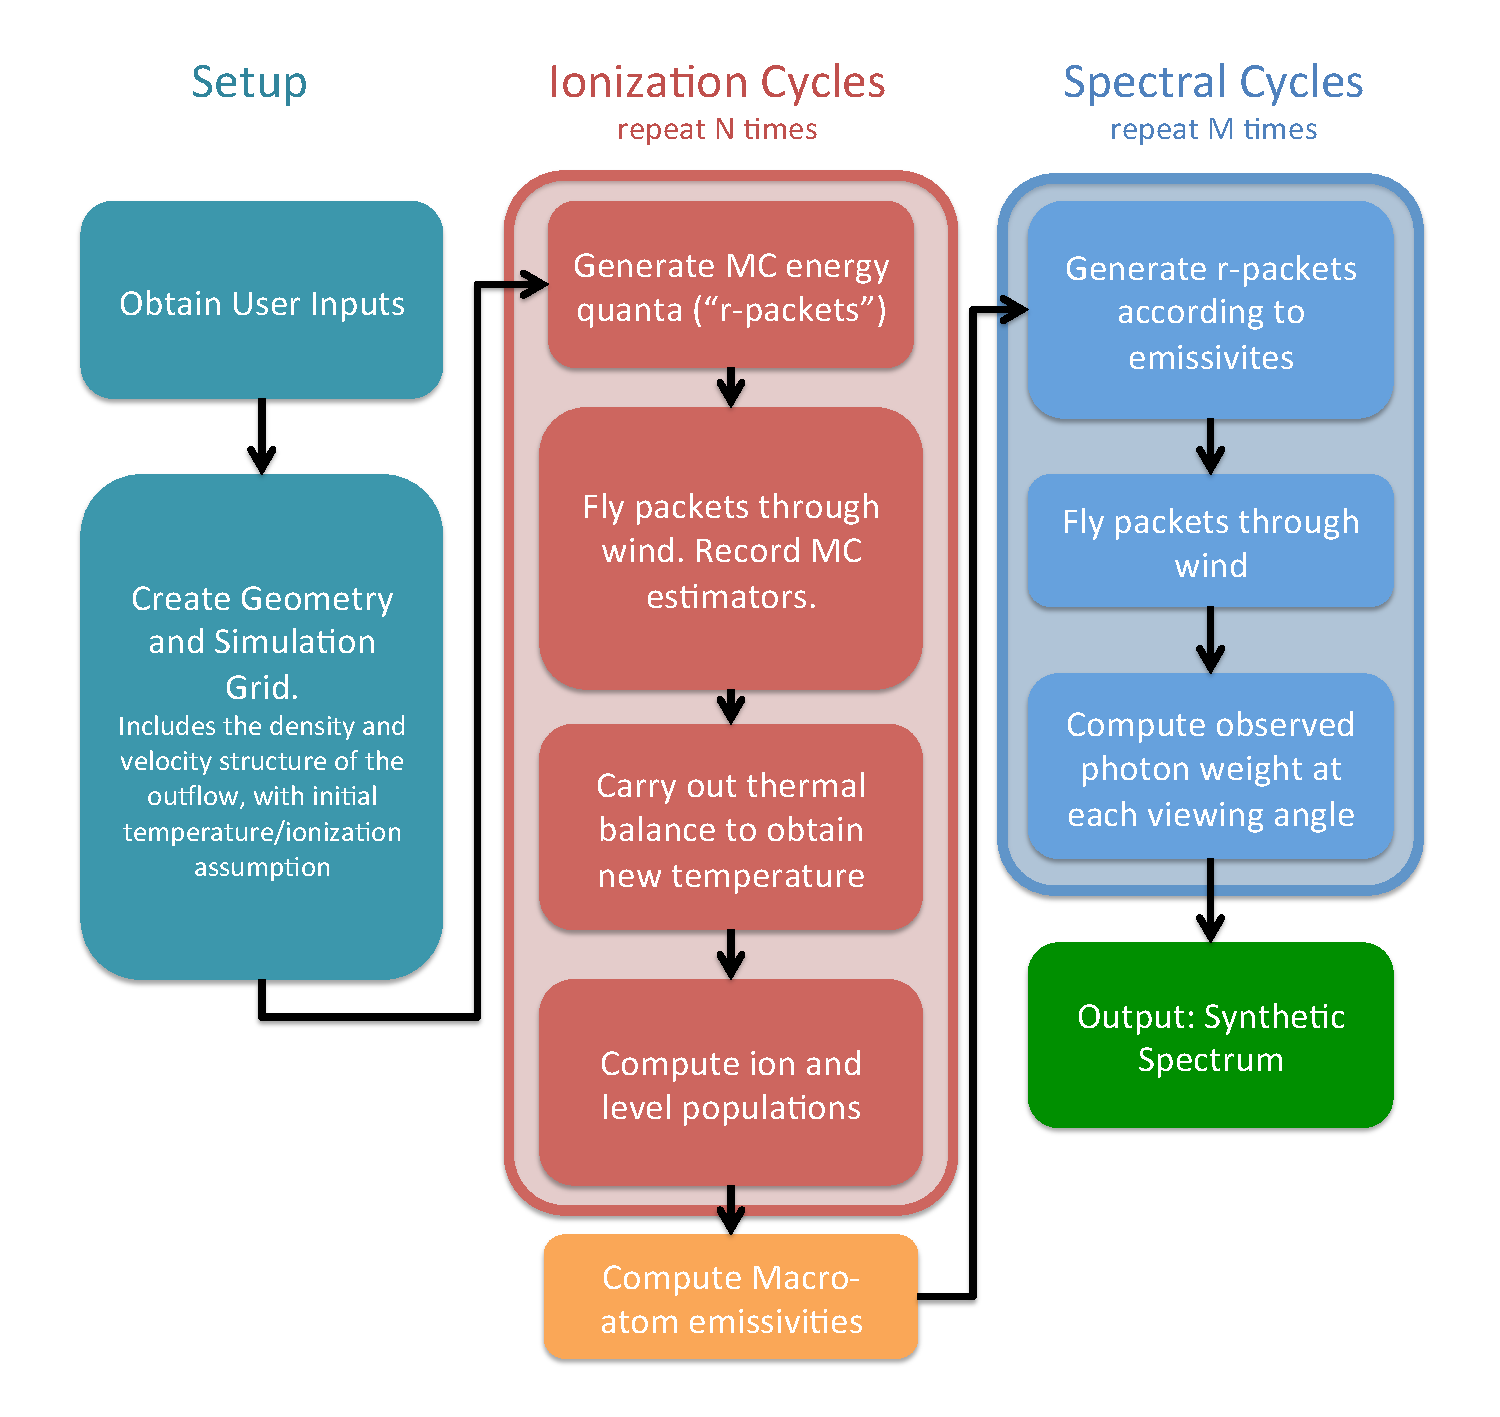
\includegraphics[width=1.0\textwidth]{figures/03-radtrans/flowchart.pdf}
\caption
{
A flowchart showing the basic operation of \py.
} 
\label{fig:flowchart}
\end{figure}

\py\ operates in three distinct stages, shown in figure~\ref{fig:flowchart}. 
First, the user specifies the photon sources,
geometry and kinematics of the system, normally with a similar parameterisation
to the SV93 model described in section~\ref{sec:sv93_model}. 
The code can operate with a number of different coordinate systems 
(e.g. spherical polar, cylindrical), but in this work I use only cylindrical coordinates.
In this case, the outflow is discretised into a $n_x \times n_z$ logarithmic grid with 
user-specified dimensions. The co-ordinates, $(x_i, z_i$), 
of the corner of the $i$th cell are then given by
\begin{align}
x_i &= L_{x}~10^{(i-1)\frac{\log (R_{\mathrm{max}} / L_{x})}{n_x}},\\
z_i &= L_{z}~10^{(i-1)\frac{\log (R_{\mathrm{max}} / L_{z})}{n_z}},
\end{align}
where $L_x$ and $L_z$ are appropriately chosen (but hardwired) scale lengths, and $R_{\mathrm{max}}$ 
is the extent of the simulation domain.
From these co-ordinates the poloidal distance can be calculated and
the velocity set according to equation~\ref{eq:v_law}. The density
is then calculated from equation~\ref{eq:rho_rz}. An initial temperature,
$T_{\mathrm{init}}$ is set by the user. The ionization fractions throughout
the wind are then initiated to Saha (LTE) abundances at $T_{\mathrm{init}}$, and the level 
populations are initially set according to the Boltzmann formula. The eventual
ionization and excitation state of a cell is insensitive to the initial assumed 
conditions providing sufficient numbers of ionization cycles are completed -- 
indeed, cells often converge on solutions with large departures from LTE.
\index{Saha equation}\index{LTE}

Once the basic setup process has been carried out, the ionization state,
level populations and temperature structure are calculated.
This is done via an iterative process, by transporting several populations of 
MC energy quanta (`photons' or `$r$-packets') through the outflow.
This process is repeated until the code converges.\index{$r$-packet}
In each of these iterations (`ionization cycles'), the code records estimators that 
characterize the radiation field in each grid cell. At the end 
of each ionization cycle, a new electron temperature is calculated
that more closely balances heating and cooling in the 
plasma. The radiative estimators and updated electron
temperature are then used to revise the ionization state of the wind,
and a new ionization cycle is started. The process is repeated until
heating and cooling are balanced throughout the wind (see sections~\ref{sec:heating_cooling}
and \ref{sec:convergence}).\index{convergence} 

This converged model provides the basis for the second set of
iterations (`spectral cycles'; section~\ref{sec:spectral_cycles}), 
in which the code computes the synthetic spectrum based on the 
MC estimators recorded during the ionization cycles. 
The emergent spectrum over the desired spectral range is synthesized by 
tracking populations of energy packets through the wind and recording 
the escaping energy packets for\index{spectrum} 
a number of user-specified viewing angles.  In the ensuing sections,
I will describe each of the above steps in more detail, particularly
with regards to the macro-atom mode of operation (section~\ref{sec:matoms}).


% \py\ is designed to operate in a number of different
% regimes, both in terms of the scale of the system and in terms of the
% characteristics of the underlying radiation field.
% It was originally developed by LK02 in order to model the UV spectra
% of CVs with a simple biconical disc wind model. SDL05
% \nocite{simmacro2005} used the code to model Brackett
% and Pfund line profiles of H in young-stellar objects (YSOs). As part
% of this effort, they implemented a `macro-atom' mode (see below) in
% order to correctly treat H recombination lines with
% \py. Finally, H13 used \py\ to model broad absorption line (BAL) QSOs. For
% this application, an improved treatment of ionization was implemented,
% so that the code is now capable of dealing with arbitrary
% photo-ionizing SEDs, including non-thermal and multi-component ones. 
\subsection{Radiation Packets}
\label{sec:packets}\index{$r$-packet} 
Every energy packet in the simulation starts out as a radiation packet generated
from one of $N_S$ photon sources. To ensure that the frequency distribution
of photons is adequately sampled in important frequency regimes, 
{\em stratified sampling} is used. A specified fraction, $f_i$,
of photons must emerge each band $i$, whose frequency boundaries
can be adapted for the astrophysical situation considered. 
The weight, $w_i$, of the radiation packets in a given energy band with boundaries
$\nu_i$ and $\nu_{i+1}$ is then given by
\begin{equation}
w_i = \frac{\sum_j^{N_S} \int_{\nu_i}^{\nu_{i+1}} L_{\nu,j}~d\nu}{f_i~N_p},
\end{equation}
where $N_p$ is the total number of photons desired, 
and $L_{\nu,j}$ is the monochromatic 
luminosity of photon source $j$. 
The frequency of photons is calculated by constructing a 
cumulative distribution function (CDF), $f_{C,i}(\nu)$,
from the spectral energy distribution in each band $i$: 
\begin{equation}
f_{C,i} (\nu) = 
\frac{\int_{\nu_i}^{\nu} L_\nu~d\nu}
{\int_{\nu_i}^{\nu_{i+1}} L_\nu~d\nu} ~.
\end{equation}
A photon frequency can then be generated by cycling through the bands. In each band,
a random number is chosen between 0 and 1, and the frequency is 
then selected by interpolating on the sampled CDF. This process is repeated until 
each band has the specified number of photons, with the packet
weights adjusted accordingly.

\py\ can operate in two modes concerning the approach to energy packets. 
In the original mode described by LK02, continuum processes attenuate 
the weight of the radiation packets. This attenuation is accounted for 
by including the wind as an additional photon source.
In the second mode, energy packets are indivisible and strict radiative equilibrium is
enforced. From here on I will only be discussing this indivisible packet scheme, 
as it is required in order to be able to use macro-atoms to accurately
treat recombination in H and He.\index{radiative equilibrium} 

\subsection{Radiative Transfer Procedure}

\label{sec:rt_procedure}
\index{Monte Carlo radiative transfer} 
As a photon travels through a plasma, it has a finite probability
of interacting with free or bound electrons and undergoing a scattering
or absorption event. In order to deal with this in a Monte Carlo sense, a random optical 
depth is generated before an $r$-packet is moved,
\begin{equation}
\tau_R = - \ln (1 - {\cal Z}),
\end{equation}
where ${\cal Z}$ is a random number between 0 and 1. 
The $r$-packet is then gradually transported through a given cell. 
As it moves, the optical depth, $\tau^\prime$, it experiences
is incremented continuously, representing continuum processes. When the $r$-packet comes
into resonance with a line, according to equation~\ref{eq:resonance},
the Sobolev optical depth is calculated from equation~\ref{eq:tau_sob} and added to 
$\tau^\prime$. This process is illustrated in Fig.~\ref{fig:scatter_ml93} and
continues until $\tau^\prime \geq \tau_R$ or the $r$-packet leaves the cell. If the
photon leaves the cell, the values of $\tau_R$ and $\tau^\prime$ are preserved,
and the process continues using the conditions in the new cell. If 
$\tau^\prime \geq \tau_R$, then an interaction with the plasma has occurred, and
the process governing this interaction must be identified. This is done by
randomly picking an interaction process in proportion with their contributions
to $\tau^\prime$. If the process is an electron scatter then a new, isotropic
direction is generated for the $r$-packet. Otherwise, the packet must
interact with either the thermal pool or the excitation energy of the plasma.

\begin{figure}
\centering
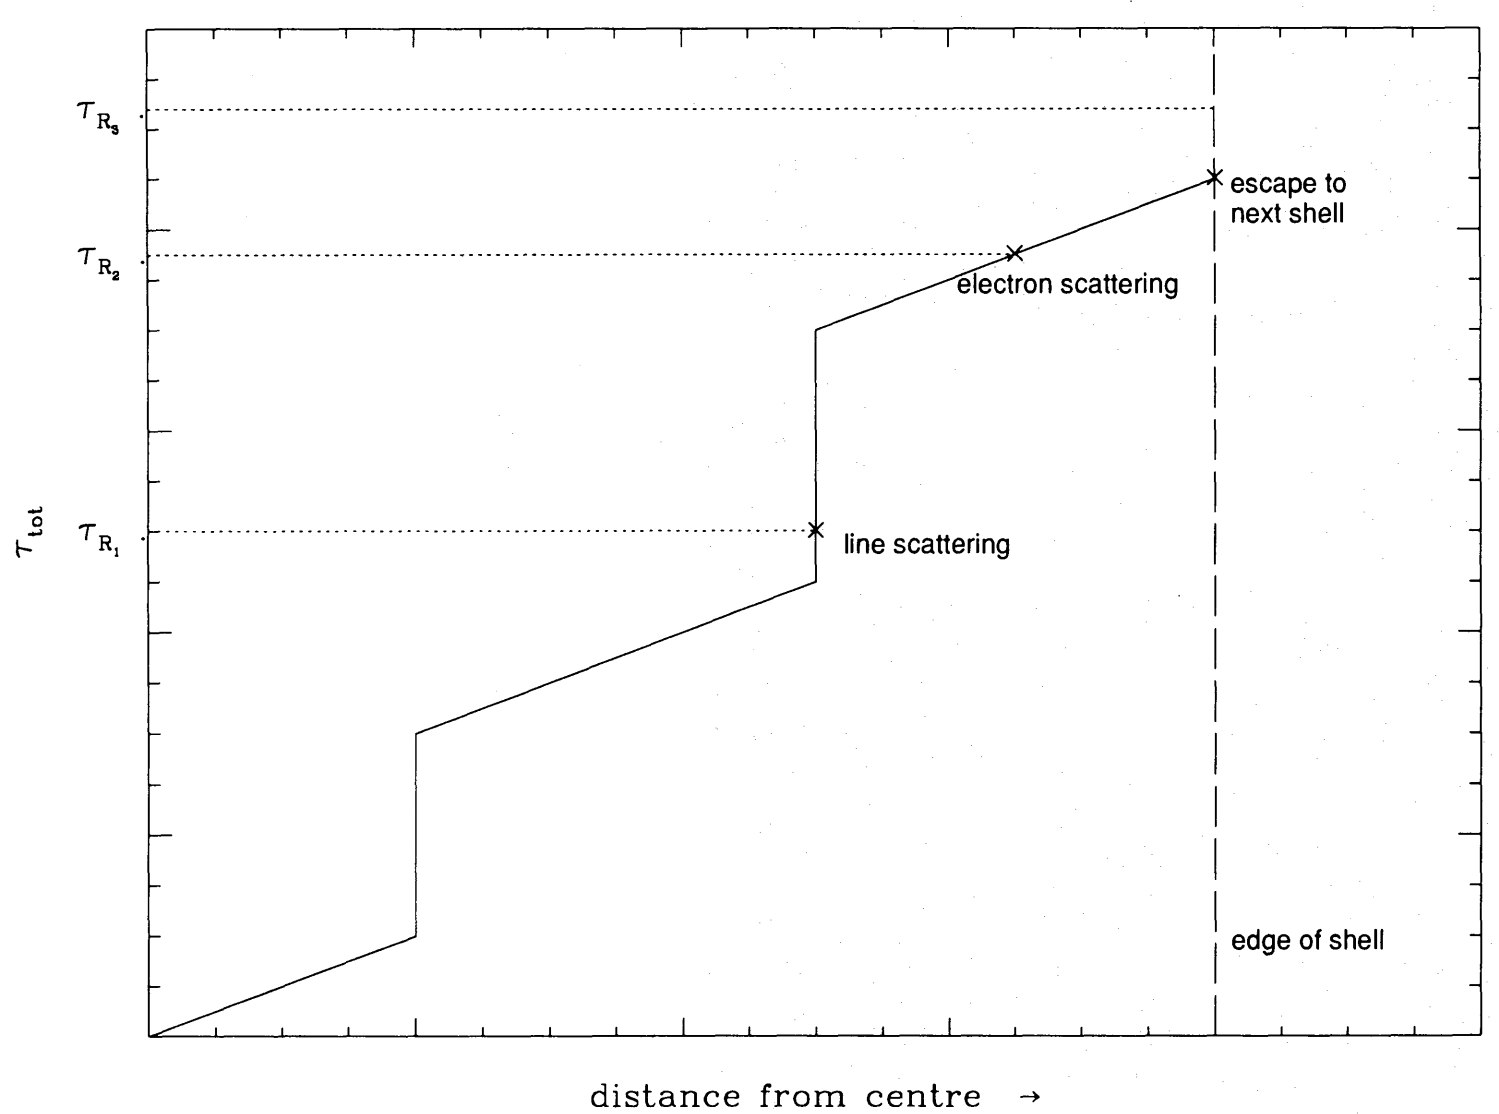
\includegraphics[width=0.7\textwidth]{figures/03-radtrans/tau_scat.png}
\caption
[The process of choosing a scattering location in a cell.]
{
{\sl Credit: Mazzali \& Lucy 1993}. 
The process of choosing a scattering location in a cell.
} 
\label{fig:scatter_ml93}
\end{figure}

\subsubsection{Continuum Opacities}

In order to calculate $\tau^\prime$ in the above approach, we need
to know the opacities that will contribute to it. An opacity 
at a given frequency, $\kappa(\nu)$,
is related to an optical depth, $\tau(\nu)$, by
\begin{equation}
\tau(\nu) = \kappa(\nu)~\Delta s,
\end{equation}
where $\Delta s$ is the distance moved by the photon. The bound-free
opacity is calculated from a sum over photoionization cross-sections (bfjumps),
such that
\begin{equation}
\kappa_{bf} = \sum_{j\kappa}^{\mathrm{bfjumps}} \sigma_{j\kappa} (\nu) n_j.
\end{equation}
The free-free emission coefficient for an individual ion $i$ of charge $Z_i$ 
is \citep{gayet1970}\index{free-free emission}\index{free-free absorption}
\begin{equation}
j_{ff,i} (\nu) = \bar{g}_{ff}\frac{8 Z_i^2 q_e^6}{3m_e^2 c^3}
\left( \frac{2\pi m_e}{3 k T_e} \right)^{1/2}
N_i n_e \exp(-h\nu/kT_e),
\label{eq:jff} 
\end{equation}
where $\bar{g}_{ff}$ is the mean free-free Gaunt factor and formally
depends on both frequency and temperature.\index{gaunt factor!free-free}
The free-free opacity is calculated from Kirchhoff's law,\index{Kirchhoff's law} 
\begin{equation}
\kappa_{ff, i}(\nu) = \frac{j_{ff,i} (\nu)}{B_\nu (T_e)}.
\end{equation}
% which gives
% \begin{equation}
% \kappa_{ff, i}(\nu) = \bar{g}_{ff} n_e N_i \frac{4}{3} \left(\frac{2\pi}{3}\right)^{1/2}~
% \frac{Z_i^2 q_e^6}{m_e^2 hc} \left(\frac{m_e}{kT_e}\right)^{1/2}~
%  \nu^{-3} [1 - \exp(-h\nu/kT_e)].
% \end{equation}
These opacities are all used in the heating and cooling estimators 
introduced in section~\ref{sec:estimators}.
For radiative transfer purposes, electron scattering is treated in the Thomson
limit\index{electron scattering}
\begin{equation}
\kappa_{es} = \sigma_T n_e.
\end{equation}
However, for heating and cooling balance the electron scattering opacity 
is treated in the Compton limit, in order to estimate the Compton heating and cooling 
effect on the plasma. The Compton opacity is given by
\begin{equation}
\kappa_{C} = \sigma_{KN} (\nu) n_e,
\end{equation}
where $\sigma_{KN} (\nu)$ is the cross-section computed 
from the Klein-Nishina formula \citep{klein-nishina} and, unlike $\sigma_T$,
is frequency dependent.\index{Compton scattering}\index{Klein-Nishina formula}

\subsubsection{Doppler Shifts}
\index{Doppler shift}
When calculating opacities, the photon frequency must be shifted from
the rest frame of the photon into the rest frame of the plasma.
This shift depends on the before and after directions of the photon. Let us denote
these two directions with unit vectors $\vec{n}_i$ and $\vec{n}_f$, respectively,
and consider a situation when a photon scatters off an electron in a region of the
wind moving at velocity $\vec{v}$.
The final frequency of the photon with initial frequency $\nu_i$ is then 
\begin{equation}
\nu_f = \nu_i ~\frac{1 - (\vec{v} \cdot \vec{n}_i) / c}{1 - (\vec{v} \cdot \vec{n}_f) / c}.
\end{equation}
In the case of a resonance scatter with line transition $u \rightarrow j$, the 
new frequency is
\begin{equation}
\nu_f = \frac{\nu_{uj}}{1 - (\vec{v} \cdot \vec{n}_f) / c}.
\end{equation}
When we consider that the resonant point is chosen according to 
equation~\ref{eq:resonance}, and that $v=\vec{v} \cdot \vec{n}_f$ in this case,
it is clear that the above two equations are equivalent. The above formulae are the 
non-relativistic case, which was used for this thesis. However, this should in general 
be improved to use the special relativistic formula.
This would produce more accurate Doppler shifts for the fastest regions of an
outflow, as the current treatment 
introduces errors of order $5$\AA\ at the blue edges of the highest velocity
absorption lines in the models described in chapters 4 and 5.



\subsubsection{Choosing Packet Directions}

The last variable, in addition to $w_i$ and $\nu$, needed to define a 
radiation packet is the direction of travel.
In the case of isotropic emission, the direction of a photon packet
is chosen so that the probability of emission in each bin of solid
angle is the same. It follows that 
\begin{equation}
p(\Omega)d\Omega \propto \cos \theta \sin \theta d\theta d\phi,
\end{equation}
where the angles are in polar coordinates and relative to the local
outward normal. For a spherical emitting source, such as 
a star, one must first generate a location on the star's surface
and then calculate the photon direction relative to the normal at the point.
For emission from optically thick surfaces the above equation can be modified
to include linear limb darkening, $\eta(\theta)$:
\begin{equation}
p(\theta, \phi) d\theta d\phi = \eta(\theta) \cos \theta \sin \theta d\theta d\phi.
\end{equation}
The Eddington approximation is usually adopted in the code, so that $\eta(\theta)$
is given by
\begin{equation}
\eta(\theta) = a (1 - \frac{3}{2} \cos \theta).
\end{equation}
The constant $a$ is normalised such that the total probability
sums to $1$. Whenever a radiation packet undergoes an electron scatter,
the new direction is chosen to be isotropic. However,
when the photon is a line photon, the new direction is chosen
according to a line trapping model, which samples a probability 
distribution according to the Sobolev escape probability in different 
directions.\index{limb darkening}


%%%%%%%%%%%%%%%%%%%%%%%%%%%%%
%MACRO ATOMS
%%%%%%%%%%%%%%%%%%%%%%%%%%%%%

%%%%%%%%%%%%%%%%%%%%%%%%%%%%%
%%%%%%%%%%%%%%%%%%%%%%%%%%%%%
% MACRO ATOMS
%%%%%%%%%%%%%%%%%%%%%%%%%%%%%
%%%%%%%%%%%%%%%%%%%%%%%%%%%%%

\section{Macro-atoms}
\label{sec:matoms}
{\sl The macro-atom scheme was created by Leon Lucy and is outlined in 
his 2002/03 papers. It was implemented in \py\ by Stuart Sim, initially
for the study of recombination lines in YSOs (SDL05).
}

\citet[][hereafter L02, L03]{lucy2002, lucy2003}
has shown that it is possible to calculate the emissivity of a gas in
statistical equilibrium without approximation for problems with large departures
from LTE.
His `macro-atom'\index{macro-atom} scheme allows for all possible transition paths from a given level,
dispensing with the two-level approximation, and
provides a full non-LTE solution\index{LTE}
for the level populations based on Monte Carlo estimators. The macro-atom
technique has already been used to model Wolf-Rayet star\index{Wolf-Rayet star}
winds \citep{sim2004}, AGN disc winds \citep{simlong2008, tatum2012},\index{YSO}\index{Supernova}
supernovae \citep{kromersim2009, kerzendorfsim} and YSOs (SDL05). A full 
description of the approach can be found in L02 and L03.\index{stellar wind}

Understanding macro-atoms requires something of a philosophical shift.
Normally MCRT is described in the most intuitive way- that is, we imagine
real photons striking atoms and either scattering or imparting energy to a 
bound electron. With Lucy's scheme we instead 
reimagine the MC quanta as packets of quantised energy flow, 
so that the scheme becomes a purely
{\em statistical} one. The amount of time a given energy quantum spends in a specific atomic
level or thermal pool is then somewhat analogous to the absolute energy 
contained therein.

Following L02, let us consider an atomic species interacting with a radiation field.
If the quantity $\epsilon_j$ represents the ionization plus excitation energy of 
a level $j$ then the rates at which the level absorbs and emits radiant energy 
are given by
\index{Macro-atoms!Rate equations}
\begin{equation}
 \dot{A}_{j}^{R} = R_{\ellp j} \epsilon_{j \ellp} \;\;\;\;\; {\rm and} \;\;\;
\;\;  \dot{E}_{j}^{R} = R_{j \ellp} \epsilon_{j \ellp} \;\;\; ,
\end{equation}
where $\epsilon_{j \ellp} = \epsilon_j - \epsilon_\ellp$.
Here, I have adopted Lucy's convention, in which the subscript 
$\ellp$ denotes a summation over all lower states ($\ell<j$), and
$\up$ a summation over all upper states ($u>j$).
Similarly, the rates corresponding to {\em kinetic} (collisional)
energy transport can then be written as
\begin{equation}
 \dot{A}_{j}^{C} = C_{\ellp j} \epsilon_{j \ellp} \;\;\;\;\; {\rm and}
\;\;\;
\;\;  \dot{E}_{j}^{C} = C_{j \ellp} \epsilon_{j \ellp} \;\;\; ,
\end{equation}
Let us define ${\cal R}$ as a total rate, such that
${\cal R}_{\ellp j}  = R_{\ellp j} + C_{\ellp j}$.
If we now impose statistical equilibrium\index{statistical equilibrium}
%
\begin{equation}
 ({\cal R}_{\ellp j}-{\cal R}_{j \ellp})+({\cal R}_{\up j}-{\cal R}_{j\up})=0 \;\;\;,
\end{equation}
we obtain 
\begin{eqnarray}
 \dot{E}_{j}^{R}+\dot{E}_{j}^{C}+{\cal R}_{j\up}\epsilon_{j}+
 {\cal R}_{j \ell}\epsilon_{\ellp}  \nonumber \\  
 = \dot{A}_{j}^{R}+\dot{A}_{j}^{C}+{\cal R}_{\up j} \epsilon_{j}
 +{\cal R}_{\ellp j} \epsilon_{\ellp}           .  
 \label{eq:matom_SE}     
\end{eqnarray}
This equation is the starting point for the macro-atom scheme. It shows 
that, when assuming radiative equilibrium, the energy flows through
a system depend only on the transition probabilities and atomic physics
associated with the levels the energy flow interacts with.
By quantising this energy flow into radiant ($r$-) and kinetic ($k$-) packets, 
we can simulate the energy transport through
a plasma discretised into volume elements (``macro-atoms''),
whose associated transition probabilities govern the interaction 
of radiant and kinetic energy with the ionization and excitation energy associated 
with the ions of the plasma.

Although equation~\ref{eq:matom_SE} assumes strict radiative equilibrium,\index{radiative equilibrium}
it is trivial to adjust it to include non-radiative source and sink terms. 
For example, in an expanding parcel of plasma, adiabatic cooling may be 
included with a simple modification to the RHS of equation~\ref{eq:matom_SE}.
\index{adiabatic cooling}


%%%%%%%%%%%%%%%%%%%%%%%%%%%%%
% PROBS
%%%%%%%%%%%%%%%%%%%%%%%%%%%%%

\subsection{Transition Probabilities}

Having interpreted equation~\ref{eq:matom_SE} in a {\em stochastic} way,
we can now construct our Monte Carlo scheme, following L02.
A macro-atom in state $j$ always has a finite probability of `deactivating'
radiatively or collisionally:
\begin{equation}
p_{j}^{R} = \dot{E}_{j}^{R} / D_j \;\;\;\;\; {\rm and} \;\;\;
\;\; p_{j}^{C} = \dot{E}_{j}^{C} / D_j,
\label{eq:deactivate}
\end{equation}
where I have defined
\begin{equation}
D_j =  \dot{E}_{j}^{R}+\dot{E}_{j}^{C}+{\cal R}_{j\up}\epsilon_{j}+
 {\cal R}_{j \ellp}\epsilon_{\ellp} = ({\cal R}_{j\ellp} + {\cal R}_{j\up}) \epsilon_{j}.
\end{equation}
The corresponding jumping probabilities\index{macro-atom!transition probability}, 
which describe the probability
that the macro-atom transitions to a different state while remaining active, 
are given by
\begin{equation}
p_{ju} = {\cal R}_{ju} \epsilon_{j} / D_j \;\;\;\;\; {\rm and} \;\;\;
\;\; p_{jl} = {\cal R}_{jl} \epsilon_{l} / D_j.
\end{equation}
Note that the jumping probability is always proportional to the energy
of the lower level, whereas the emission probability is proportional
to the energy {\em difference} between the levels, as 
$\dot{E}_{j}^{R} = R_{j\ellp} (\epsilon_j - \epsilon_\ellp)$. We can also
trivially show that the probabilities are correctly normalised, as
\begin{align}
p_{j}^{R} + p_{j}^{C} + p_{jl} + p_{ju} &=
(1/D_j) ( {\cal R}_{j\up} \epsilon_{j} + {\cal R}_{j\ellp} \epsilon_{\ellp} +
\dot{E}_{j}^{R} + \dot{E}_{j}^{C}) \\
&= 1. \nonumber
\end{align}

With these transition
probabilities identified, a Monte Carlo calculation can proceed by formulating
the normal statistical equilibrium rate equations that will depend on
the ambient conditions of the plasma. The effect of these ambient conditions
is expressed through the use of Monte Carlo estimators.




%%%%%%%%%%%%%%%%%%%%%%%%%%%%%
% RATES
%%%%%%%%%%%%%%%%%%%%%%%%%%%%%
\subsection{Rate equations}
\label{sec:rate_eq}\index{Monte Carlo!estimator}
The macroscopic transition probabilities above depend on the traditional
rate equations formulated according to statistical equilibrium. 
In the framework of the Sobolev escape probability formalism\index{Sobolev approximation} 
(see section~\ref{sec:sobolev}),\index{radiative excitation}\index{radiative de-excitation}
the bound-bound excitation rate, ${\cal R}_{ju}$, in an ion is given by 
\begin{equation}
{\cal R}_{ju} = B_{ju} n_j J_{\mathrm{est}} \left(1 - \frac{n_j g_u}{n_u g_j} \right) + q_{ju} n_j n_e,
\label{eq:rju}
\end{equation}
where $u$ is now a specific upper level, and $q_{ju}$ is the collisional
rate coefficient (see section~\ref{sec:coll}). The $(1 - n_j g_u/n_u g_j)$ term
is the correction for stimulated emission from equation~\ref{eq:einstein_relations},
and requires that there are no population inversions (see section~\ref{sec:numerical_matom}).
The quantity $J_{\mathrm{est}}$ is the Monte Carlo estimator for the mean intensity 
impinging on the Sobolev region, weighted by an angle-dependent escape probability, 
given by \citep{sim2004}
\begin{equation}
J_{\mathrm{est}} = \frac{c}{4 \pi \nu_{uj} V} \sum_{i}^{\mathrm{photons}} w_i \frac{1 - e^{-\tau_{s,i}}}{\tau_{s,i}} \frac{1}{(dv/ds)_i}.
\end{equation}
Here $w_i$ is the photon weight (in luminosity units), $\nu_{uj}$
is the line frequency, $dv/ds$ is the velocity gradient and
$\tau_s$ is the Sobolev optical depth.
The sum is over all photons that come into resonance with the line,
and thus represents an integral over solid angle.
This is essentially the MC estimator form of $\beta_{uj}\bar{J}_{uj}$, and
reduces to the estimator in equation~20 of L02 
in the limit of homologous flow or symmetric escape probabilities.
The corresponding de-excitation rate is then \index{Sobolev approximation}
\begin{equation}
{\cal R}_{uj} = \beta_{ju} A_{uj} n_u + B_{uj} n_u J_{\mathrm{est}}  +
q_{uj} n_u n_e.
\label{eq:ruj}
\end{equation}
The photoionization and collisional ionization rates
between a lower level, $l$, and the continuum level $\kappa$ 
(or, in the case of ions with more than one bound electron, 
the ground state of the upper ion),
$\kappa$, are
\begin{equation}
{\cal R}_{j \kappa}= \gamma_{j\kappa} n_j - \alpha^{st}_{\kappa j} n_\kappa n_e   + q_{j \kappa} n_j n_e.
\label{eq:rjk}
\end{equation}
Here, $q_{j \kappa}$ is the collisional ionization rate coefficient,\index{collisional ionization}
$\gamma_{j \kappa}$ is the photoionization rate\index{photoionization}
from $j \rightarrow \kappa$, and $\alpha^{st}_{\kappa j}$ is the stimulated recombination
coefficient. This is included as a negative photoionization term rather 
than a positive recombination term as in L03, which requires that there are
no population inversions (see section~\ref{sec:numerical_matom}). 
The corresponding recombination rate is given by\index{recombination}
\begin{equation}
{\cal R}_{\kappa j} = \alpha_{\kappa j} n_{\kappa} n_e + q_{\kappa j}
n_\kappa n_e, \\
\end{equation}
where $\alpha_{\kappa l}$ is the radiative recombination coefficient
to level $l$, and is given by 
\begin{equation}
\alpha_{\kappa j} = 4\pi \left( \frac{n_j}{n_e n_\kappa} \right)^*_{T_e} \int^\infty_{\nu_0} 
\frac{\sigma_{j\kappa} (\nu)}{h \nu} \frac{2 h \nu^3}{c^2} 
\exp \left( \frac{- h \nu}{k T_e} \right) d\nu.
\label{eq:alpha_sp}
\end{equation}
This treatment means that radiative and collisional
rates to and from all levels can be considered when calculating the
ionization state, level populations and transition probabilities, 
although ionization directly to excited levels of the upper ion is 
neglected.\index{level population}

\subsubsection{Collision Strengths}
\label{sec:coll}

The bound-bound collisional de-excitation rate coefficient, $q_{uj}$, is calculated from the
\cite{vanregemorter} approximation, given by\index{bound-bound collision strength}
\begin{equation}
q_{uj} = \bar{g} f_{ju}\frac{8.629\times10^{-6}}{g_u T_e^{1/2}}
\frac{8 \pi}{\sqrt{3}}~\frac{g_j}{g_u} \frac{\nu_{\mathrm{Ryd}}}{\nu_{uj}}
\label{eq:vanregemorter}
\end{equation}
where $\lambda_{uj}$ is the wavelength of the transition, $\nu_{\mathrm{Ryd}}$
is the frequency at $13.6$~eV and $\bar{g}$ is 
an effective gaunt factor of order unity.
The inverse rate is calculated by considering detailed balance, 
such that
\begin{equation}
q_{ju} = q_{uj} \frac{g_u}{g_j} \exp \left( \frac{-h \nu_{uj}}{k T_e} \right).
\label{eq:vanregemorter2}
\end{equation}\index{bound-bound collision strength}
Using equation~\ref{eq:vanregemorter} means that collisions between radiatively
forbidden transitions are not taken into account when one 
splits levels into $l$- and $s$-subshells, as well
as principal quantum number, $n$ (as done with He~\textsc{i}; 
for the CV models in chapter 4). Although this approximation is, in general, 
a poor one, the effect is second order in the physical 
regime where recombination lines are formed in the models presented here 
(see section~\ref{sec:coll_bl}).\index{van Regemorter approximation} 

The bound-free collision strengths are calculated using equation~5.79 of
\cite{mihalas}. The collisional ionization rate coefficient is\index{collisional ionization}
\begin{equation}
q_{j\kappa} = 1.55 \times 10^{-13} n_e~\bar{g}_{i}~\sigma_{j\kappa} (\nu_{\kappa j})~
\frac{h \nu_{\kappa j}}{k T_e^{3/2}}
\exp \left( \frac{- h \nu_{\kappa j}}{k T_e} \right),
\label{eq:qioniz}
\end{equation}
where $\sigma_{j\kappa} (\nu_{\kappa j})$ is the photoionization cross-section 
at the threshold energy.
The effective gaunt factor for ion $i$, $\bar{g}_{i}$, is approximately
equal to $0.1,0.2,0.3$ for $Z=1,2$ and $>2$, respectively,
where $Z$ is the atomic number. Note that the use of this estimator
implies a $\nu^{-3}$ shape to the photoionization cross-section,
which is only strictly true for for hydrogenic ions.
The collisional (three-body) recombination rate is found using the Saha equation
and given by\index{collisional recombination}\index{Saha equation}
\begin{equation}
q_{\kappa j} = q_{j\kappa} \left( \frac{n_j}{n_e n_\kappa} \right)^*_{T_e}.
\label{eq:qrecomb}
\end{equation}
For numerical reasons, the above two expressions are combined in \py\ where 
possible, in order to avoid multiplying two exponentials.
\index{recombination}




%%%%%%%%%%%%%%%%%%%%%%%%%%%%%
%ESTIMATORS
%%%%%%%%%%%%%%%%%%%%%%%%%%%%%
\subsection{Macro-atom estimators}
\label{sec:estimators}
In order to solve the above rate equations and compute the transition 
probabilities, it is necessary to construct estimators for the various properties
of the radiation field that appear in the macro-atom rate equations. This is done
by converting integrals over the radiation field into summations over 
$r$-packets passing through a cell. This represents the stochastic nature of
a MC simulation and is by no means unique to the macro-atom formalism.
The first step is to apply the energy-density argument of \cite{lucy1999radeq},
which gives, for a time-independent code\index{Monte Carlo!estimator}
\begin{equation}
J_\nu~d\nu = \frac{1}{4\pi}\frac{1}{V} \sum_{d\nu} w_i \Delta s,
\end{equation}
\index{mean intensity}
where the summation is over all photons between $(\nu, \nu+d\nu)$. This allows
the formulation of estimators in a MC sense, rather than in integral form. 

\subsubsection{Bound-free estimators}
The estimator for the photoionization rate is\index{photoionization rate}\index{photoionization}
\begin{equation}
\gamma_{j\kappa} = \frac{1}{V} \sum_i^{\mathrm{photons}} 
\frac{w_i~\sigma_{j\kappa}({\nu})}{h \nu}~\Delta s
\end{equation}
and that for the stimulated recombination\index{stimulated recombination} rate is
\begin{equation}
\alpha_{\kappa j}^{st} =\left( \frac{n_j}{n_e n_\kappa} \right)^*_{T_e}
\frac{1}{V} \sum_i^{\mathrm{photons}} 
\frac{w_i~\sigma_{j\kappa}({\nu})}{h \nu}
~\exp(-h\nu/kT_e)~\Delta s,
\end{equation}
where $\sigma_{j\kappa} (\nu)$ is the photoionization cross-section for this transition.
We also need to define modified rate coefficients to represent
the rates at which bound-free transitions add energy to, and remove energy from, 
the radiation field. These are required for photoionization, 
spontaneous recombination and stimulated recombination and are given by\index{recombination}

\begin{equation}
\gamma^E_{j\kappa} = \frac{1}{V} \sum_i^{\mathrm{photons}} 
\frac{w_i~\sigma_{j\kappa}}{h \nu_{\kappa j}}~\Delta s, 
\end{equation}

\begin{equation}
\alpha^E_{\kappa j} = 4\pi \left( \frac{n_j}{n_e n_\kappa} \right)^*_{T_e}
 \int^\infty_{\nu_{\kappa j}} 
\frac{\sigma_{j \kappa}(\nu)}{h \nu_{\kappa j}} \frac{2 h \nu^3}{c^2} 
\exp \left( \frac{- h \nu}{k T_e} \right) d\nu,
\end{equation}

\begin{equation}
\alpha_{\kappa j}^{st,E} = \left( \frac{n_j}{n_e n_\kappa} \right)^*_{T_e}
\frac{1}{V} \sum_i^{\mathrm{photons}}
\frac{w_i~\sigma_{j\kappa}({\nu})}{h \nu_{\kappa j}}
~\exp(-h\nu/kT_e)~\Delta s.
\end{equation}
The rate at which recombinations convert
thermal {\em and} ionization energy into radiant energy is then
$\alpha^E h\nu_{\kappa j} n_\kappa n_e$, where $h \nu_{\kappa j}$
the energy difference between the continuum state $\kappa$ and 
the level $j$ the electron is recombining into. 
The amount of this energy which is removed from the thermal pool
therefore given by the estimator\index{recombination}
\begin{equation}
\cc_{bf} = \sum_{j\kappa}^{\mathrm{bfjumps}} 
\left[ (\alpha^E_{\kappa j} + \alpha^{st,E}_{\kappa j} - \alpha_{\kappa j} - \alpha^{st}_{\kappa j}) 
n_{\kappa} + 
q_{j\kappa} n_j \right]
n_e h\nu_{\kappa j} V,
\end{equation}
where the sum is over all the macro-atom bound-free transitions ($j\rightarrow\kappa$) 
in the simulation, set by
the number of photoionization cross-sections. 
For bound-free heating\index{bound-free heating}, a similar expression can be derived. The rate at which
a level $j$ absorbs energy by bound-free 
transitions is given by $\gamma^E_{j\kappa} h\nu_{\kappa j} n_\kappa n_e$,
of which $\gamma_{j\kappa} h \nu_{\kappa j} n_l$ goes into ionization energy, leaving 
\begin{equation}
\hh_{bf} = \sum_{j\kappa}^{\mathrm{bfjumps}} \left[ (\gamma^E_{\kappa j} - \gamma_{\kappa j}) n_j + n_\kappa n_e^2 q_{\kappa j} \right] h \nu_{\kappa j} V
\end{equation}
as the rate at which radiant energy heats the plasma via bound-free transitions.


\subsubsection{Bound-bound estimators}
The heating and cooling rates for macro-atom bound-bound transitions are the rates of
collisional excitations and de-excitations
- i.e. the rate at which thermal energy is converted into
bound-bound excitation energy and vice versa.
These heating and cooling rate estimators are:\index{bound-bound heating}\index{bound-bound cooling}

\begin{equation}
\hh_{bb} = \sum_{ju}^{\mathrm{lines}} q_{uj} n_u n_e h \nu_{uj} V,
\end{equation}


\begin{equation}
\cc_{bb} = \sum_{ju}^{\mathrm{lines}} q_{ju} n_j n_e h \nu_{uj} V.
\end{equation}

\subsubsection{Other heating and cooling estimators}
Although I have now defined the estimators required to calculate the 
transition probabilities, level populations, heating rates and cooling rates in macro-atoms, 
there are still a number of heating and cooling mechanisms that do not involve macro-atoms. 

The free-free cooling estimator is calculated from the emission coefficient
in equation~\ref{eq:jff},\index{free-free cooling}
\begin{equation}
\cc_{ff} = V \sum_i^{\mathrm{ions}} \int \frac{j_{ff,i}(\nu)}{4\pi} d\nu,
\end{equation}
where the integral is over all frequencies included in the simulation,
and the sum is also over all ions included in the simulation.
The corresponding heating rate is then\index{free-free heating}
\begin{equation}
\hh_{ff} = \sum_i^{\mathrm{photons}} w_i \kappa_{ff} \Delta s.
\end{equation}
Compton heating and cooling is included in the thermal balance and as
$(r\rightarrow k)$ and $(k\rightarrow r)$ transitions:\index{Compton heating}
\begin{equation}
\cc_{\mathrm{comp}} = 16 \pi \sigma_T V J \frac{k T_e}{m_e c^2},
\end{equation}
\begin{equation}
\hh_{\mathrm{comp}} = n_e \sum_i^{\mathrm{photons}} \frac{h\nu}{m_e c^2} w_i \kappa_{C}\Delta s,
\end{equation}
where the estimator for the frequency-integrated mean intensity is\index{mean intensity}
\begin{equation}
J = \frac{1}{4\pi V} \sum_i^{\mathrm{photons}} w_i \Delta s.
\label{eq:j}
\end{equation}
Induced Compton heating is then given by \citep{cloudy2013}\index{Compton heating!induced}
\begin{equation}
\hh_{\mathrm{ind~comp}} = n_e \sum_i^{\mathrm{photons}} \frac{J_\nu c^2}{h \nu^3} \frac{h\nu}{m_e c^2} 
w_i \kappa_{C} \Delta s,
\end{equation}
where $J_\nu c^2/h \nu^3$ represents the
photon occupation number, and $J_\nu$ is either 
calculated from the spectral model
described in section~\ref{sec:simple_ionization} or from a dilute blackbody.
The adiabatic cooling rate is derived by considering the $PdV$ work done by the flow
and is given by\index{adiabatic cooling}
\begin{equation}
\cc_{a} = k T_e V (\nabla \cdot v) \left(n_e + \sum\limits_{i=1}^{\mathrm{ions}} N_i\right),
\end{equation}
where $\nabla \cdot v$ is the divergence of the 
velocity field at the centre of the cell. The sum is over all ions 
included in the simulation.

\noindent

%%%%%%%%%%%%%%%%%%%%%%%%%%%%%
% K PACKETS
%%%%%%%%%%%%%%%%%%%%%%%%%%%%%
\subsection{$k$-packets}\index{$k$-packet}
$k$-packets represent quantised kinetic or thermal energy, and any interaction
chain involving a $k$-packet thus represents interaction with the thermal
pool of ions and electrons. $k$-packets can be produced either directly
via a continuum heating process ($r \rightarrow k$), 
or by the collisional de-activation of a macro-atom 
($r \rightarrow \ldots \rightarrow A^* \rightarrow k$) in accordance with
equation~\ref{eq:deactivate}. 

Once they are produced, $k$-packets never move, as they represent the quantised
thermal energy flow in a finite volume element. Hence, when they are produced,
their destruction path is decided according to the different cooling mechanisms
in the plasma. A $k$-packet then has a probability of being destroyed by process $i$ that
is given by
\begin{equation}
p_{i,\mathrm{destruct}} = \cc_i / (\cc_{bf} + \cc_{ff} + \cc_{bb} + \cc_{\mathrm{comp}} + \cc_a).
\end{equation}
Note that only adiabatic cooling leads to an actual destruction of the energy packet,
as a departure from radiative equilibrium. All other processes will lead to the 
creation of an active macro-atom or an $r$-packet.\index{adiabatic cooling}


%%%%%%%%%%%%%%%%%%%%%%%%%%%%%
% FLOWCHART
%%%%%%%%%%%%%%%%%%%%%%%%%%%%%

\subsection{Putting it All Together}

I have now defined all quantities needed to write down the transition 
probabilities in a macro-atom simulation. Fig.~\ref{fig:flow_matom}
shows the decision tree traversed by an energy packet in the simulation,
showing the complicated set of interactions it can undergo each time it 
scatters.\index{macro-atom}

\begin{figure}
\centering
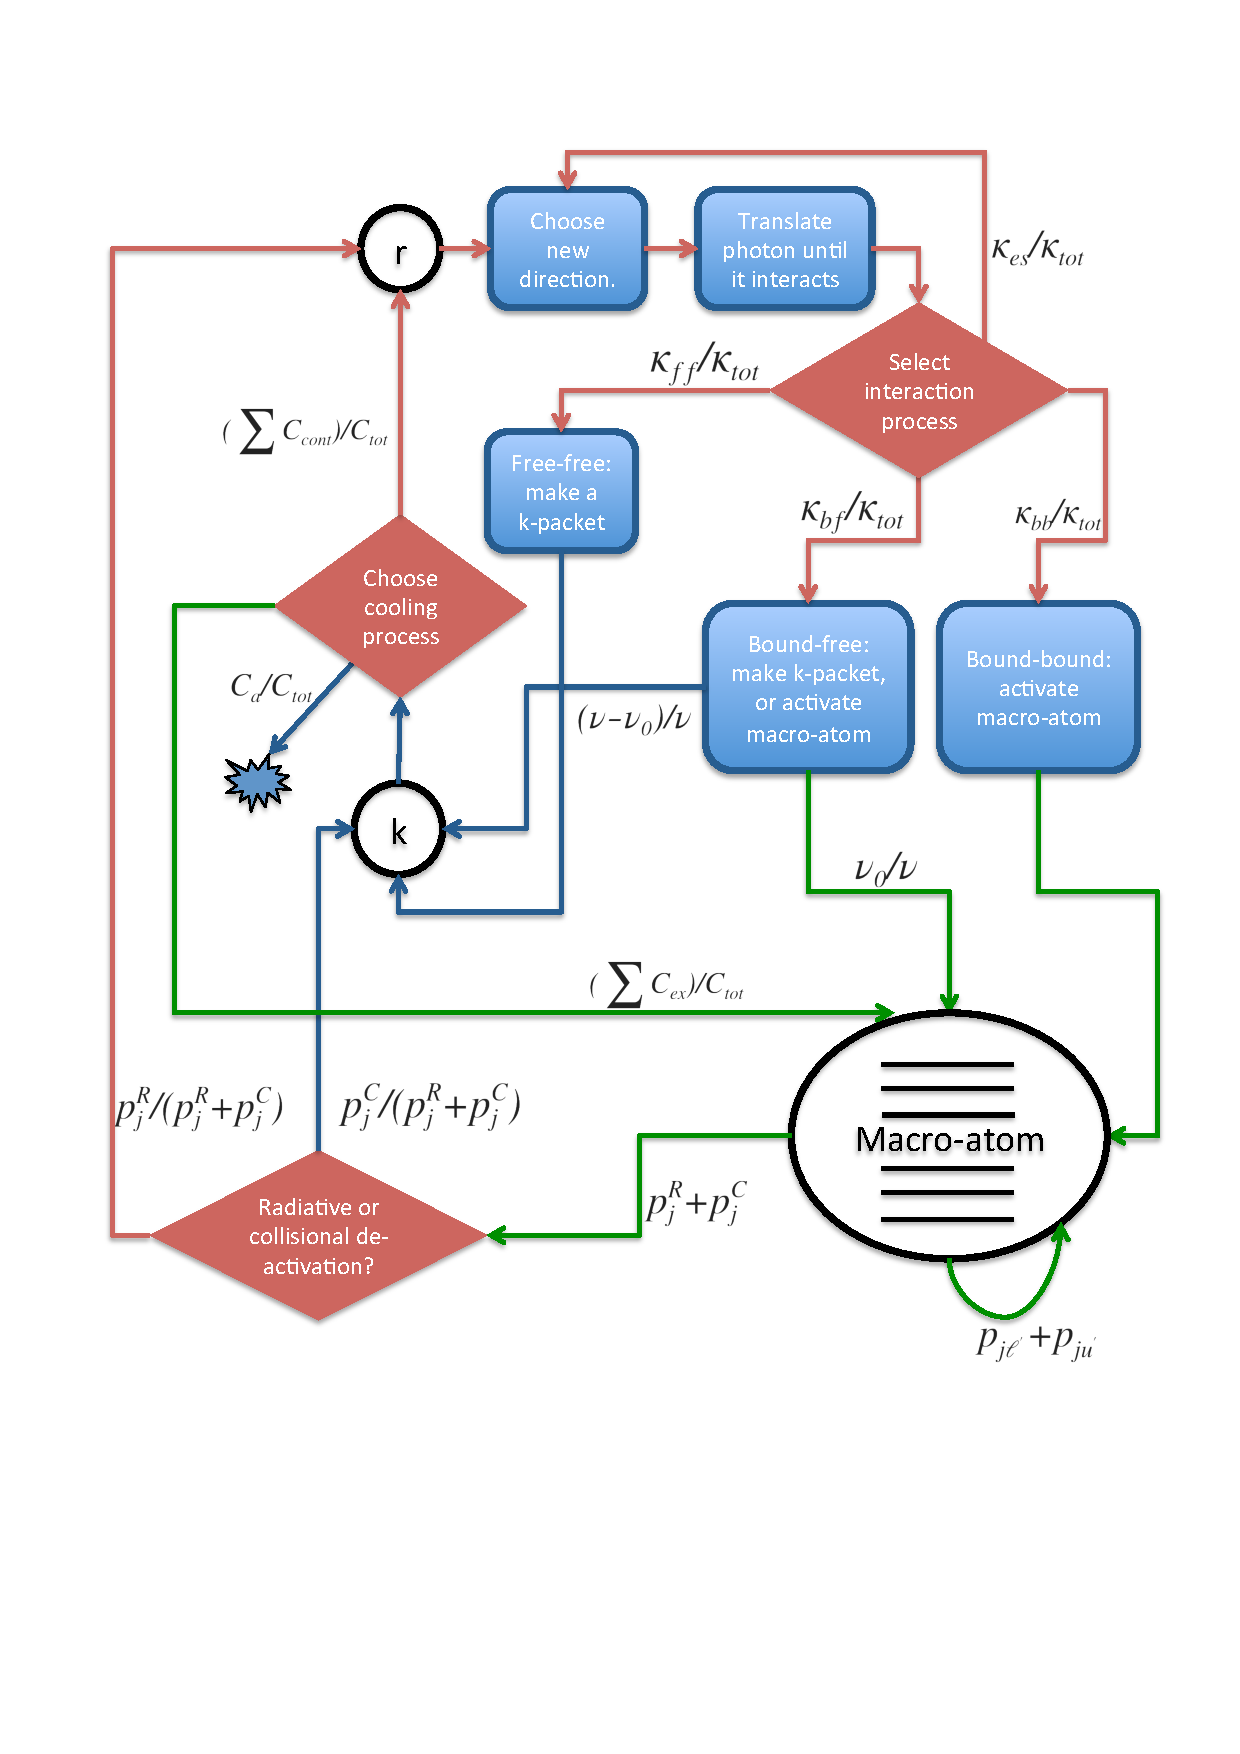
\includegraphics[width=1.0\textwidth, clip=true, trim=0 2.6in 0in 0in ]{figures/03-radtrans/matom_flow_ca.pdf}
\caption
[The decision tree traversed by an energy packet 
in macro-atom mode.]
{
The decision tree traversed by an energy packet 
in macro-atom mode, depicting the interaction
between radiation ($r$-packets), the thermal pool ($k$-packets), and ionization
and ionization/excitation energy (macro-atoms). 
The probabilities at each decision point are 
marked, and are defined in the text. The red, blue and green coloured arrows
represent radiant, kinetic and ionization/excitation energy respectively.
The symbols are defined in the text, except ${\cal C}_{\mathrm{cont}}$ and 
${\cal C}_{\mathrm{ex}}$ which refer to cooling contributions to radiative and excitation 
energy respectively.
} 
\label{fig:flow_matom}
\end{figure}

%% XXX CHECK THIS.


%%%%%%%%%%%%%%%%%%%%%%%%%%%%%
% POPS
%%%%%%%%%%%%%%%%%%%%%%%%%%%%%


\subsection{Ionization Fractions and Level Populations}
\label{sec:matom_pops}
In section~\ref{sec:lte} I described how it is possible to calculate the
ionization and excitation of a plasma under LTE or dilute approximations.
Macro-atoms are not approximated -- their level and ion populations are 
calculated by solving the rate equations formulated in section~\ref{sec:rate_eq}. 
This is done via matrix inversion. For an element with $n$ ions and $m_i$
levels in each ion, we construct a square matrix with dimensions 
$m = \sum_i^n m_i$.
This element then has a total number density of $N_{elem} = \sum_i^n N_i$.
In order to turn the system of rate equations for this element into matrix form, we
populate the $j$th diagonal of the matrix with the negative of the rate out of
level $j$, $-({\cal R}_{j\ellp} + {\cal R}_{j\up})$, 
and populate the off-diagonals $(j,k)$ with the positive rate 
${\cal R}_{jk}$. These are then multiplied by a vector containing the fractional level
populations and must equal a vector of zeros, due to statistical equilibrium.
Our matrix equation is then\index{ionization state}\index{level population}
%
\begin{equation}
\begin{bmatrix}
    -{\cal R}_{1\up} & {\cal R}_{21} & {\cal R}_{31} & \dots & {\cal R}_{m1} \\
    {\cal R}_{12} & -({\cal R}_{2\ellp} + {\cal R}_{2\up}) & {\cal R}_{32} & \dots & {\cal R}_{m2} \\
    {\cal R}_{13}  & {\cal R}_{23} & -({\cal R}_{3\ellp} + {\cal R}_{3\up}) & \dots & {\cal R}_{m3} \\
    \vdots & \vdots & \vdots & \ddots & \vdots \\
    {\cal R}_{1m}      & {\cal R}_{2m} & {\cal R}_{3m} & \dots & -{\cal R}_{m\ellp}
\end{bmatrix}
\begin{bmatrix}
    n_1 / N_{elem} \\
    n_2 / N_{elem} \\
    n_3 / N_{elem} \\
    \vdots         \\
    n_m / N_{elem} 
\end{bmatrix}
=
\begin{bmatrix}
    0 \\
    0 \\
    0 \\
    \vdots \\
    0
\end{bmatrix}
.
\end{equation}
%
This problem is not yet soluble, as a valid solution is that all levels 
could simply have occupation numbers of $0$. In order to close the problem, we must impose the boundary condition that the sum of the fractional populations is 1, i.e.
%
\begin{equation}
\sum_i \frac{N_i}{N_{elem}} = 1.
\end{equation}
In matrix form, this is equivalent to replacing the entire first row
of the rate matrix with 1, and the first entry of the RHS vector with a 1,
so that we have
%
\begin{equation}
\begin{bmatrix}
    1  & 1 & 1 & \dots & 1\\
    {\cal R}_{12} & -({\cal R}_{2\ellp} + {\cal R}_{2\up}) & {\cal R}_{32} & \dots & {\cal R}_{m2} \\
    {\cal R}_{13}  & {\cal R}_{23} & -({\cal R}_{3\ellp} + {\cal R}_{3\up}) & \dots & {\cal R}_{m3} \\
    \vdots & \vdots & \vdots & \ddots & \vdots \\
    {\cal R}_{1m}      & {\cal R}_{2m} & {\cal R}_{3m} & \dots & -{\cal R}_{m\ellp}
\end{bmatrix}
\begin{bmatrix}
    n_1 / N_{elem} \\
    n_2 / N_{elem} \\
    n_3 / N_{elem} \\
    \vdots         \\
    n_m / N_{elem} 
\end{bmatrix}
=
\begin{bmatrix}
    1 \\
    0 \\
    0 \\
    \vdots \\
    0
\end{bmatrix}
\end{equation}
%
This matrix equation can now be solved.
The actual matrix manipulation in the code is handled by the GNU 
scientific libraries \citep[GSL;][]{GSL} implementation of
LU decomposition \citep{turing}. This is a fast and reliable way of
inverting large matrices that includes error handling and enables
checking of, for example, singular rate matrices.
\index{LU decomposition}

\subsection{Numerical Issues and Population Inversions}
\label{sec:numerical_matom}

An inherent problem in MC simulations is noise, particularly
when the MC estimators involved rely on specific frequencies of
photons in order to be incremented. One of the side effects
of this is that population inversions can occur. A population
inversion is present when\index{population inversion}\index{Monte Carlo!estimator}
\begin{equation}
n_u > n_l \frac{g_u}{g_l}.
\label{eq:pop_inverse}
\end{equation}
This can cause problems, for example, with the inclusion
of stimulated recombination rates as negative photoionization
terms. Inspection of equations~\ref{eq:rju} 
and \ref{eq:rjk} reveals that a negative
excitation rate would be obtained in this situation.

In order to prevent this problem, the level populations are `cleaned' 
after each matrix calculation, as suggested by L03. 
This is done by cycling through the levels
after the calculation has been carried out and checking if
condition~\ref{eq:pop_inverse} is ever satisfied. If it is, then
the upper population is simply set to a value just below this limit.
This is only necessary when there is a permitted dipole transition 
between the two levels being compared.

In addition to the population inversion problem, it is also possible to 
produce singular rate matrixes when photon statistics are poor, 
particularly in heavily absorbed portions of the wind. 
% where photons
% which come into resonance with lines, or are above threshold frequencies,
% may be rare. 
In order to deal with this issue, I have written a routine in \py\
that checks if the rate matrix is singular and if any anomalous (negative or
non-finite) populations exist in the solution found. If either of these 
conditions are met, the calculation is redone using dilute estimators.
This procedure is also carried out for the simple-atom ionization
calculation when the rate matrix approach is in use 
(see section~\ref{sec:simple_ionization}).

%%%%%%%%%%%%%%%%%%%%%%%%%%%%%
%SIMPLE ATOMS
%%%%%%%%%%%%%%%%%%%%%%%%%%%%%

\section{A hybrid line transfer scheme: including simple-atoms}

I have now described in detail how the macro-atom approach is 
implemented in \py. A pure macro-atom approach can be easily used for
some situations -- for example, in the YSO application described by 
SDL05, which uses a H-only model. However, in accretion
disc winds, the densities can be very high, and higher $Z$ elements must be 
included. Including all these elements as macro-atoms is not
currently computationally feasible in \py\ for anything but the simplest
models. I will thus now describe a `hybrid scheme', which treats H and He
with the macro-atom approach, but models all other atoms 
as `simple-atoms'. \index{simple-atom}

\subsection{Line Transfer}

Simple-atoms still interact with $r$- and $k$-packets,
but do not possess internal transition probabilities. As a result,
they are analogous to the two-level atom treatment, as any excitation
is immediately followed by a deactivation into an $r$- or $k$-packet.
The choice of radiative or kinetic deactivation is made according 
to the relative rates in the two-level atom formalism. 
For a bound-bound transition $u\rightarrow j$, these two probabilities
are then
\begin{equation}
p_{uj}^{S,R} = \frac{ A_{uj} \beta_{uj} }
{ A_{uj} \beta_{uj} + C_{uj} \exp(-h\nu_{uj} / k T_e) }
= 1 - q
\end{equation}
and
\begin{equation}
p_{uj}^{S,C} = \frac{ C_{uj} \exp(-h\nu_{uj} / k T_e) }
{ A_{uj} \beta_{uj} + C_{uj} \exp(-h\nu_{uj} / k T_e) }
= q.
\end{equation}
For a bound-free transition, the code assumes radiative recombination, and 
thus any bound-free simple-atom activation is immediately followed 
by the creation of an $r$-packet. This approximates the bound-free continuunm, 
even when compared to other two-level atom radiative transfer schemes. 
This is discussed further and tested in section~\ref{sec:line_test}.

This hybrid approach preserves the fast treatment 
of, for example, UV resonance lines, while accurately 
modelling the recombination cascades that populate the levels 
responsible for, e.g., H and He line emission. As a result of this hybrid
scheme, a separate set of estimators must be recorded for simple-atoms, 
and the ionization and excitation of these elements is calculated 
with a different, approximate approach.
In order to include simple-atoms, we must add in a few extra pathways
to Fig.~\ref{fig:flow_matom}, so that energy packets can also
activate simple-atoms, through either bound-free or bound-bound
processes. The relative probabilities of these channels are set
in proportion with the simple-atom opacities.


\subsection{Heating and Cooling Estimators}
\label{sec:simple_hc}

The bound-bound heating rate is computed during the photon propagation and is a sum
over photons which come into resonance with each line, given by 
\begin{equation}
{\cal H}_{bb}^S = \sum_i^{\mathrm{photons}} \sum^{\mathrm{lines}}_{ju} (1 - q) (1 - e^{-\tau_{S,ju}}) w_i.
\end{equation}
Similarly, the bound-bound cooling rate is given by 
\index{bound-bound heating}\index{bound-bound cooling}
\begin{equation}
{\cal C}_{bb}^S = \sum_{ju}^{\mathrm{lines}} q \left(n_j\frac{g_u}{g_j} - n_u\right) q_{uj} n_e 
\frac{(1 - e^{-h\nu_{ju}/kT_e})}{(e^{h\nu_{ju}/kT_e} - 1)}  h \nu_{ju}.
\end{equation}
These estimators are fundamentally different quantities from the corresponding
macro-atom estimators and are not used to
calculate k-packet probabilities. Instead, they represent the amount of
energy transferred to and from the plasma by the radiation field,
whereas in the macro-atom case they represent the rate of collisional excitations
and de-excitations.
%%note the difference to the macro-atom approach- here this is already 
\noindent
The bound-free heating rate is given by
\begin{equation}
{\cal H}_{bf}^S = \sum_i^{\mathrm{photons}} \sum_{j\kappa}^{\mathrm{bfjumps}} w_{i} e^{-\tau} \frac{\nu - \nu_{j\kappa}}{\nu}
\end{equation}
where $\nu$ is the frequency of the photon in question, and $\nu_{j\kappa}$
is the ionization threshold. The bound-free cooling rate is then
\begin{equation}
{\cal C}_{bf}^S = \sum_{j\kappa}^{\mathrm{bfjumps}} \int_{\nu_{j \kappa}}^\infty
h \nu \left(\frac{2 \pi m_e k T_e}{h^2} \right)^{-3/2}
\frac{2 h \nu^3}{c^2} 
\frac{g_j}{g_\kappa g_e}
T_e^{-3/2} \sigma_{j \kappa} (\nu) 
\exp(- h (\nu - \nu_{j \kappa}) / kT_e).
\end{equation}

\subsubsection{Radiation Field Estimators, Ionization and Excitation}
\label{sec:simple_ionization}\index{ionization state}
\index{mean intensity}\index{Monte Carlo!estimator}
For simple-atoms we do not record radiation field estimators for discrete 
transitions, as we do for macro-atoms. Instead, we record estimators to
give us a model of the radiation field. The estimators needed
depend on the ionization mode employed.
The radiation temperature, $T_R$, is estimated by first recording the mean frequency, 
$\bar{\nu}$, of the photons passing through a cell
\begin{equation}
\bar{\nu} = \frac{\sum_{photons} w_i \nu_i \Delta s}{\sum_{photons} w_i \Delta s}.
\end{equation}
This is then used to estimate a radiation temperature by
considering the value expected from a blackbody \citep{ML93}:\index{blackbody}
\begin{equation}
T_r = \frac{h\bar{\nu}}{3.832~k}
\end{equation}
The dilution factor can be calculated by comparing the estimator for the mean intensity (equation~\ref{eq:j}) to the Stefan-Boltzmann law:\index{dilution factor}\index{mean intensity}
\begin{equation}
W = \frac{\pi J}{\sigma~T_r^4}.
\end{equation}
This set of estimators is sufficient to describe the 
radiation field if the dilute approximation is adopted(section~\ref{sec:dilute}).
\index{dilute approximation}

H13 improved on the dilute blackbody approximation by
modelling the SED in the cell using a series of band-limited 
radiation field estimators. In this scheme, a series of bands is defined
in which to record these estimators. These bands are different to those
discussed in section~\ref{sec:packets}, as those instead govern photon generation.
In H13, the band-limited estimators were used to construct a correction factor
that could be used in a modified Saha equation 
(similar in form to equation~\ref{eq:ml93}). However, the code has now been
improved further, so that the ion populations are computed by solving the rate equations.
Thus we now simply need to calculate photoionization rate estimators for simple 
ions, which rely on being able to integrate a modelled form of the mean intensity.

The mean intensity is modelled in each band $i$ using either a power law or exponential
with respective forms of
\begin{equation}
J_{\nu,i} = K_{PL} \nu^{\alpha_{PL}}~\mathrm{and}
\end{equation}
\begin{equation}
J_{\nu,i} = K_{\exp} \exp(-h\nu / k T_{\exp}),
\end{equation}
where $T_{\exp}$ and $\alpha_{PL}$ are fit parameters, and $K_{PL}$ and $K_{\exp}$ 
are normalisation constants, which are obtained by ensuring that
the model reproduces the band limited mean intensity from equation~\ref{eq:j}.
An example of a modeled spectrum compared to the recorded MC spectrum from
the summed photons is shown in figure~\ref{fig:cell_spec}, showing how
this scheme faithfully reproduces the SED in situations where there are large departures
from a blackbody. 

\begin{figure}
\centering
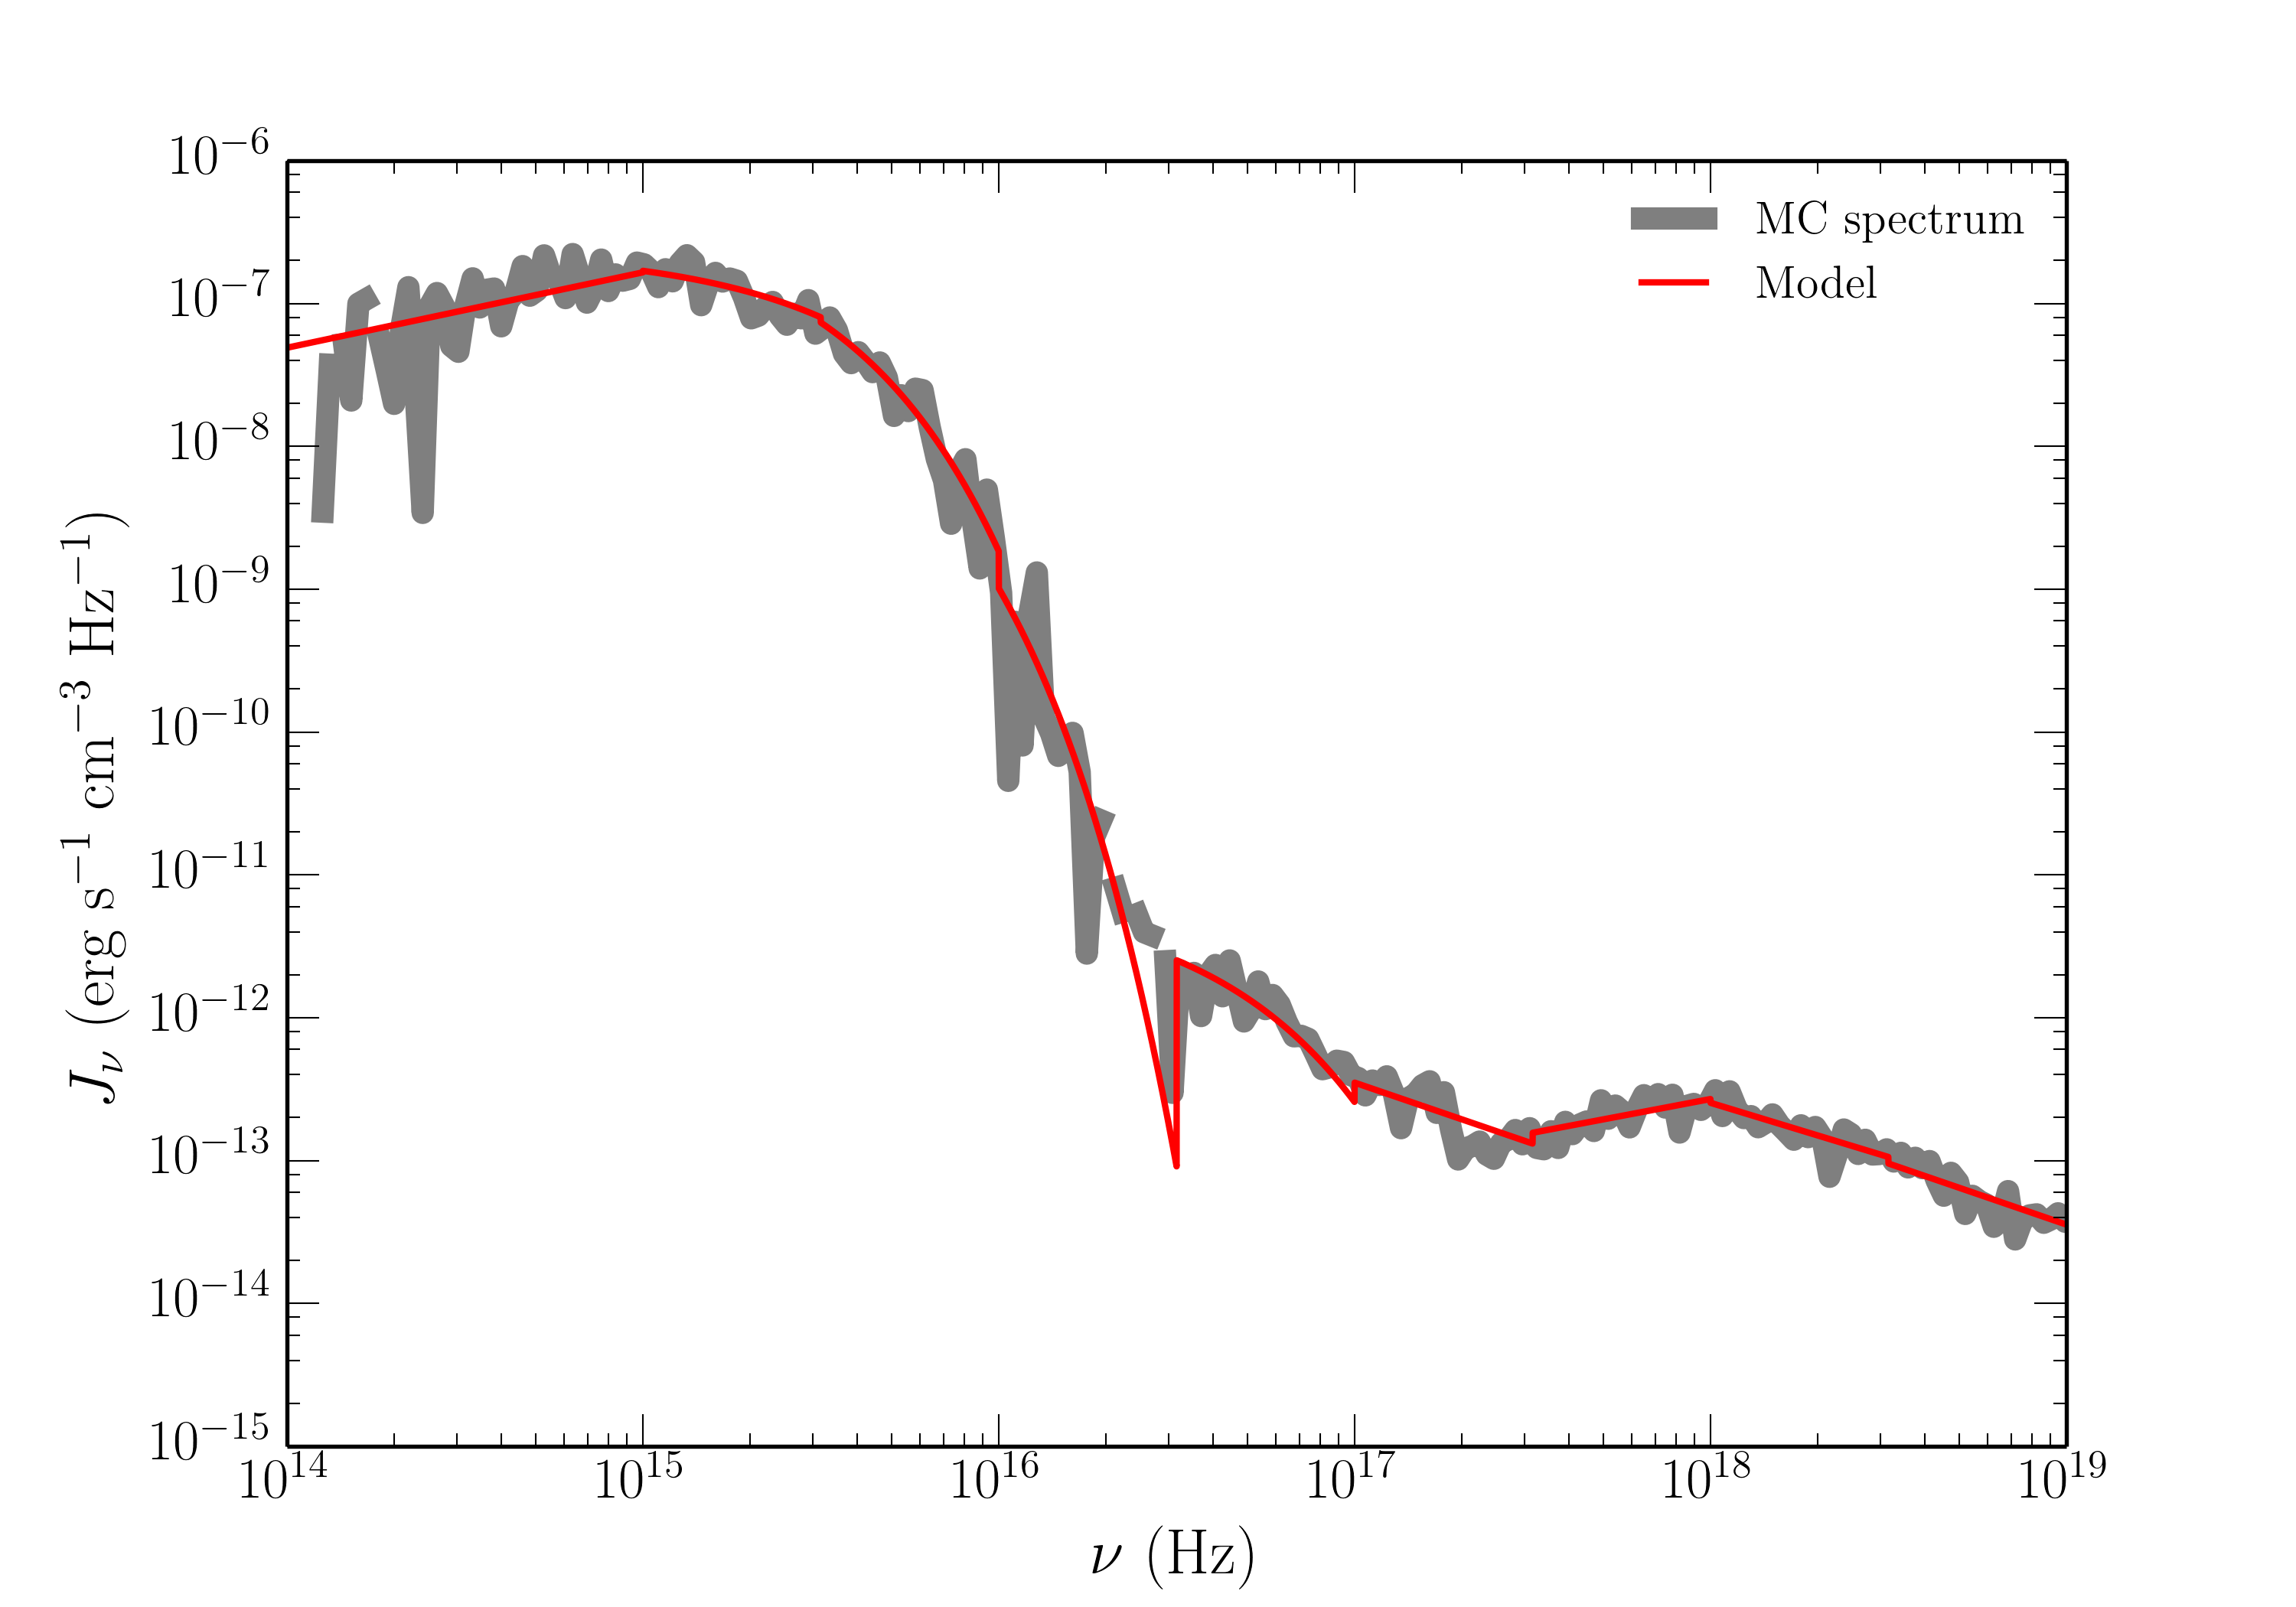
\includegraphics[width=1.0\textwidth]{figures/03-radtrans/cell_spec.png}
\caption
{
An example of a modeled spectrum in \py\ compared to the recorded MC spectrum,
from an individual cell in an AGN model.
} 
\label{fig:cell_spec}
\end{figure}

Once the model for the mean intensity has been calculated, it is possible
to formulate a photoionization rate estimator from ion $i$ to $i+1$ 
for simple-atoms,
\begin{equation}
\gamma_{i,i+1}^S = \sum_i^{\mathrm{bands}} \int_{\nu_i}^{\nu_{i+1}} 
\sum_j^{\mathrm{levels}} \frac{J_{\nu,i} \sigma_{j\kappa}(\nu) }{h \nu} d\nu.
\end{equation}
Recombination rate coefficients are then obtained from 
either tabulated data (see section~\ref{sec:atomic_data})
or, failing that, the Milne relation (equation~\ref{eq:alpha_sp}).
\index{recombination}\index{photoionization}

The rate matrix used to calculated the ionization state of simple-atoms
can now be populated. An example rate matrix for H and He would be
\begin{equation}
\begin{bmatrix}
    1  & 1 & 0 & 0 & 0 \\
    \gamma_{H\textsc{i},H\textsc{ii}}^S & -n_e \alpha_{H\textsc{ii},H\textsc{i}} & 0 & 0 & 0 \\
     0 & 0 & 1 & 1 & 1 \\
     0 & 0 & \gamma_{He\textsc{i},He\textsc{ii}}^S & -n_e \alpha_{He\textsc{ii},He\textsc{i}} - \gamma_{He\textsc{ii},He\textsc{iii}}^S & 0\\
     0 & 0 & 0 & \gamma_{He\textsc{ii},He\textsc{iii}}^S & -n_e \alpha_{He\textsc{iii},He\textsc{ii}}
\end{bmatrix}
\begin{bmatrix}
    N_{H\textsc{i}} \\
    N_{H\textsc{ii}} \\
    N_{He\textsc{i}} \\
    N_{He\textsc{ii}} \\
    N_{He\textsc{iii}} 
\end{bmatrix}
=
\begin{bmatrix}
    n_H \\
    0 \\
    n_{He} \\  
    0 \\
    0
\end{bmatrix}
.
\end{equation}
Thus the problem is very similar to solving for level populations in macro-atoms, except that
it is bounded differently.

The rate matrix method with a banded spectral model for the mean intensity is used
in chapter 5 of this thesis, whereas for chapter 4 the dilute approximation is adopted
and ion fractions are obtained from a modified Saha equation (equation~\ref{eq:ml93}).
Regardless of the ionization mode used, the relative excitation fractions of simple-atoms
within each ionization stage of a given species are 
estimated via a modified (dilute) Boltzmann
equation (equation~\ref{eq:dilute_boltzmann}). This equation is approximate, and, in 
general, this approximation is not good. We therefore endeavour to treat any species in
which the excitation state of the ions is thought to be important
in determining either the ionizing radiation field, or emergent spectrum,
as macro-atoms.\index{Saha equation}\index{dilute approximation}\index{mean intensity}

\section{Heating And Cooling Balance}
\label{sec:heating_cooling}
I have already given the estimators used to calculate
heating and cooling rates in the plasma. These are not only used
in the creation and elimination of $k$-packets, but also in the heating
and cooling balance carried out in \py\ to achieve a self-consistent
temperature structure in the wind. \index{$k$-packet}

At the end of each ionization cycle, the code has stored a new set
of MC estimators for radiative heating of the plasma. We then
assume that each cell is in thermal equilibrium, so that the appropriate
electron temperature is simply the value of $T_e$ that is a solution
to the equation
\begin{equation}
\hh_{\mathrm{tot}} - \cc_{\mathrm{tot}} ( T_e) = 0,
\end{equation}
where $\hh_{\mathrm{tot}}$ and $\cc_{\mathrm{tot}}$ are the total heating and cooling rates in 
the plasma. A number of checks are in place to ensure numerical stability,
namely a maximum temperature and a maximum change in temperature from cycle
to cycle. This is especially important in cases where the initial
guess at the wind temperature is far from the true value.

\subsection{Convergence}

\label{sec:convergence}
\index{convergence}
\py\ always runs a fixed number of ionization cycles, rather than terminating
when a convergence criterion is reached. As a result, it is up to the user
to check that the simulation is converged. An individual cell is considered
converged when a) the temperature stops changing signicantly, i.e. both
$T_R$ and $T_e$ satisfy
\begin{equation}
\frac{|T_{\mathrm{new}} - T_{\mathrm{old}}|}{T_{\mathrm{new}} + T_{\mathrm{old}}} < 0.05,
\end{equation}
and b) the heating and cooling rates are well balanced, such that
\begin{equation}
\frac{|\hh_{\mathrm{tot}} - \cc_{\mathrm{tot}}|}{\hh_{\mathrm{tot}} + \cc_{\mathrm{tot}}} < 0.05.
\end{equation}
These criteria could doubtless be improved, but they are nonetheless
a good way of ensuring that thermal and radiative equilibrium holds in the 
plasma. An example of how the average temperature and fraction
of converged cells changes over the course of the ionization cycles in
a typical CV model is shown in Fig.~\ref{fig:conv}.


\begin{figure}
\centering
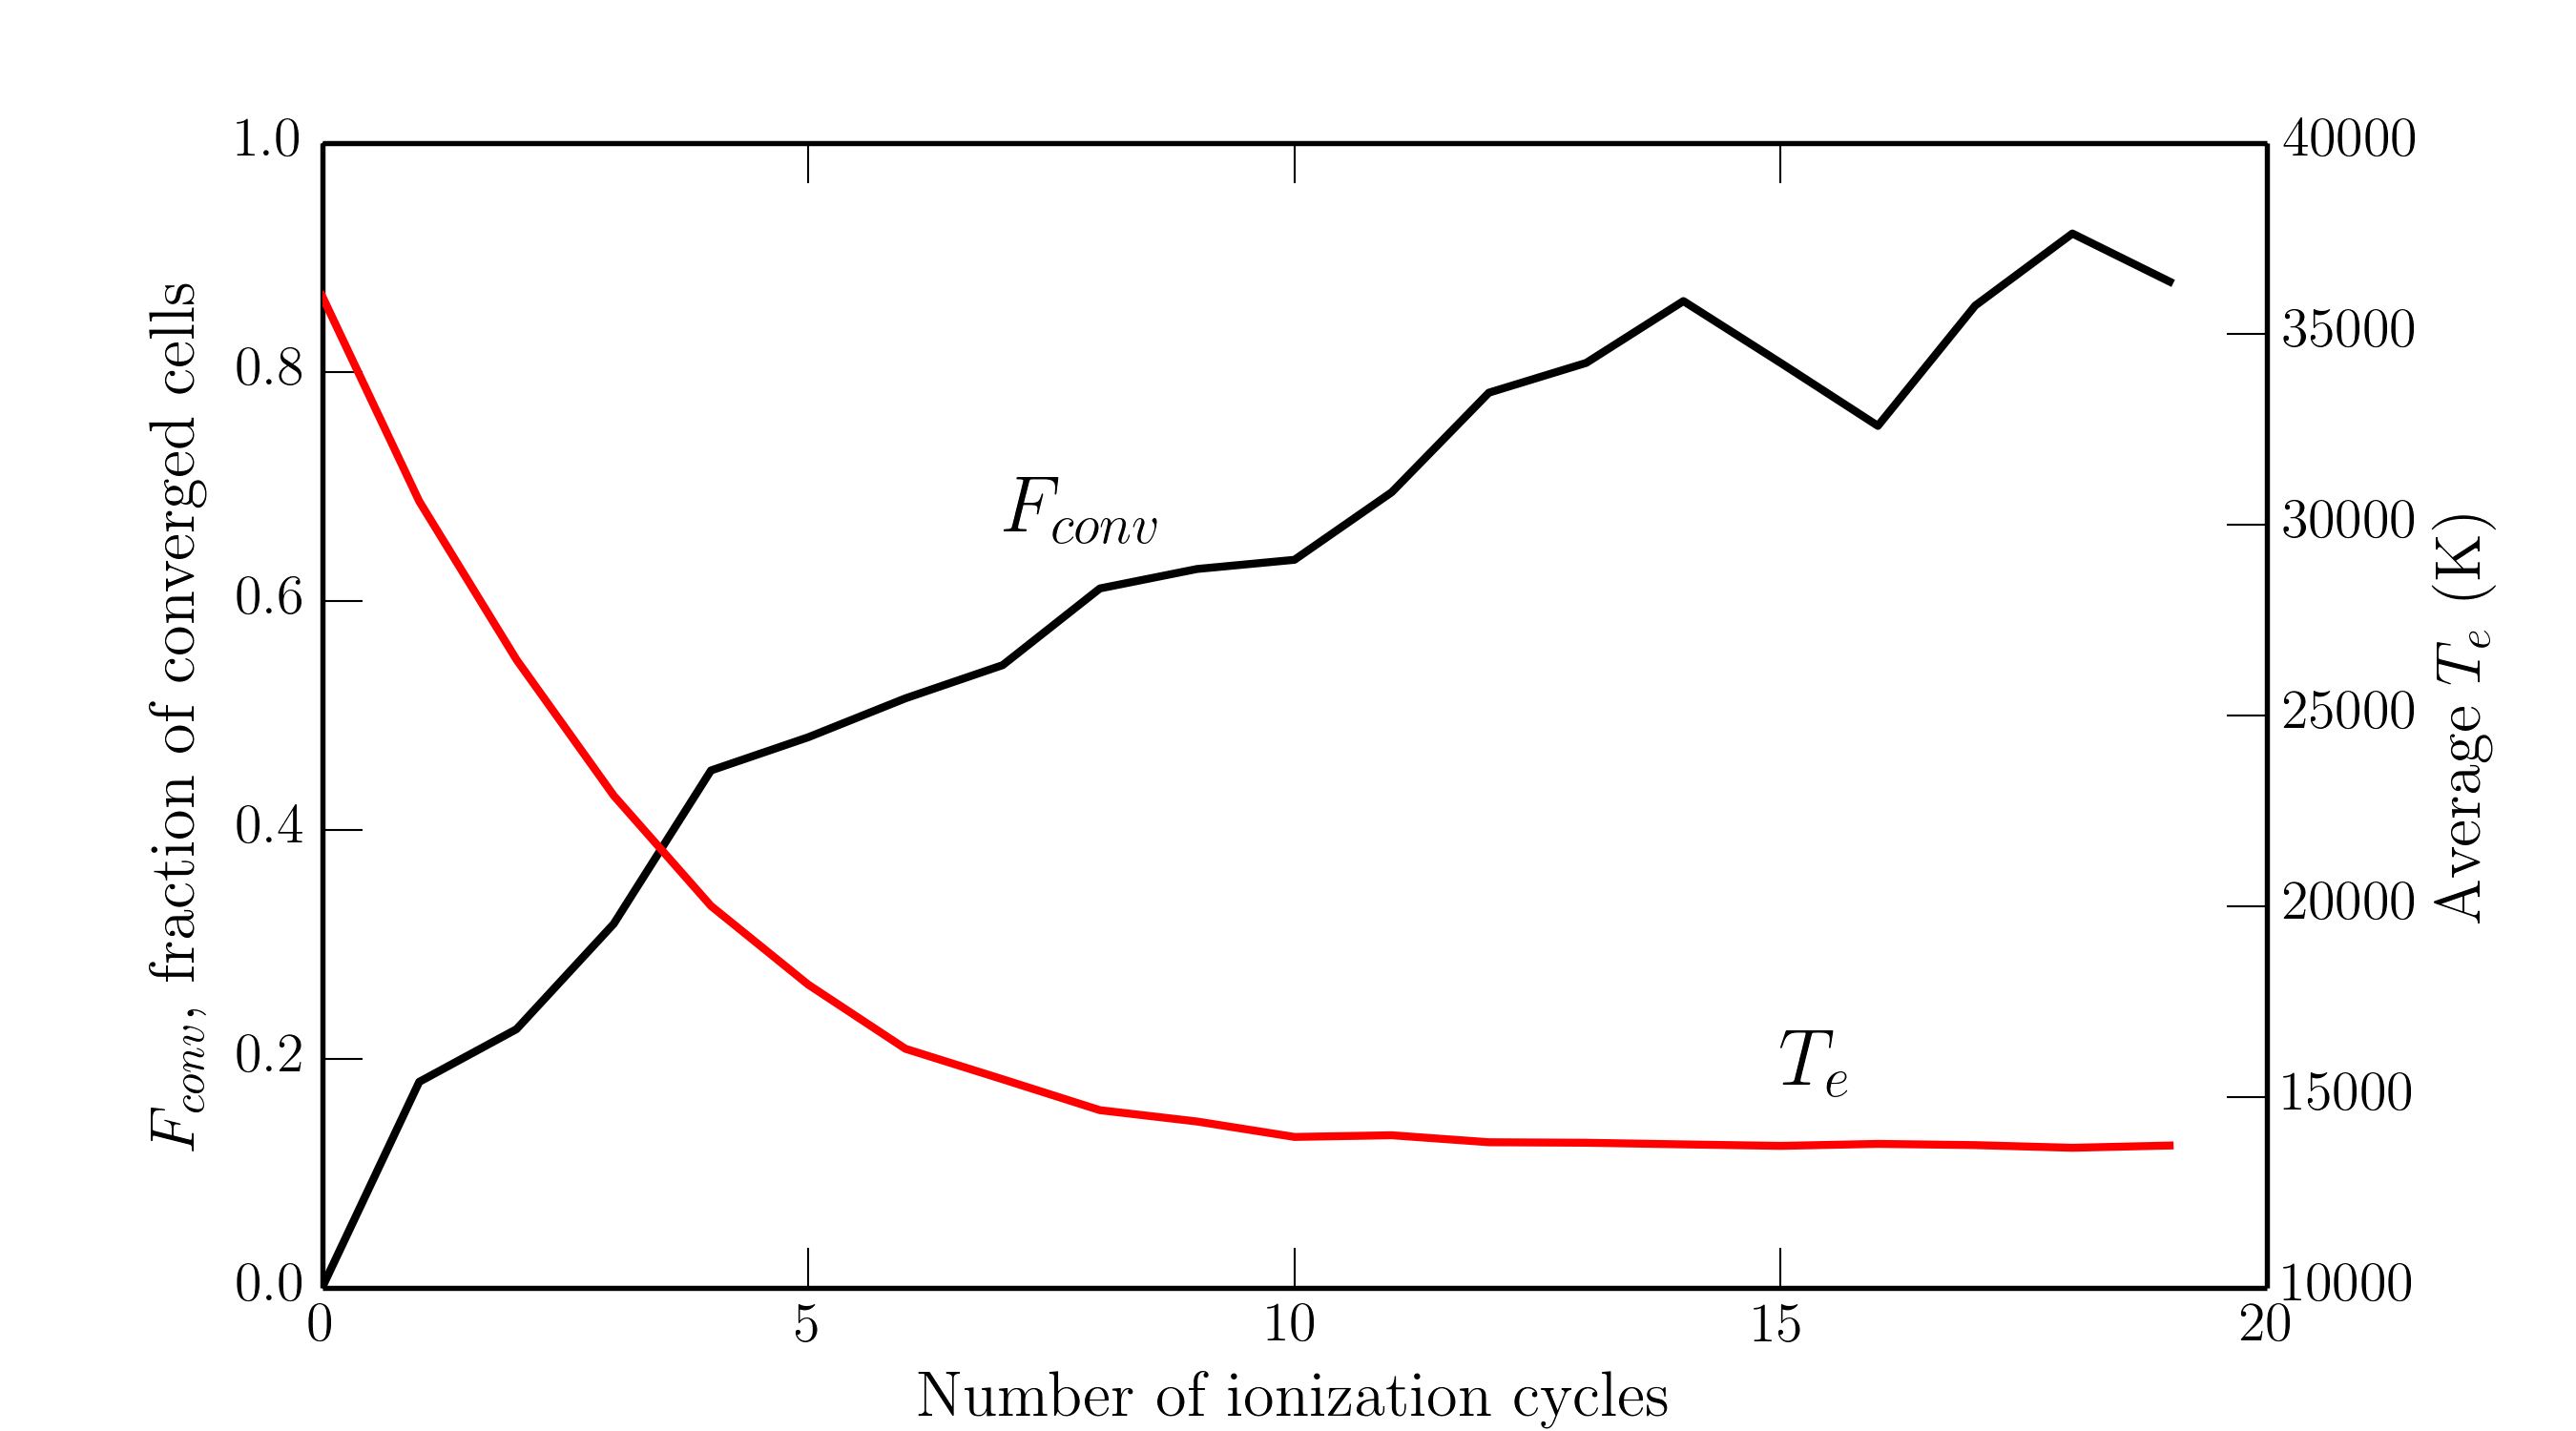
\includegraphics[width=1.0\textwidth]{figures/03-radtrans/graph_conv.png}
\caption
{
The average temperature and fraction of converged cells in
a typical CV model, shown as a function of the number of ionization cycles
completed. 
} 
\label{fig:conv}
\end{figure}




\section{Spectral Cycles}
\label{sec:spectral_cycles}
The primary output from \py\ is a synthetic spectrum over a specific wavelength
range produced at user-specified viewing angles. This spectrum is produced 
in a separate cycle from the calculation of the ionization state, as we are then concerned
with producing detailed, high-resolution spectra in a specific wavelength regime
that can then be compared to observations.

\index{variance reduction}
The code utilises a variance reduction technique in order to minimise the amount of 
time spent in this portion of the code. This technique is based 
on a similar method implemented by \cite{woods1991} and is known in the code
as the `extract' method. This method works by 
tracking photon packets until they scatter or interact with the plasma, according
to the procedure described in section~\ref{sec:rt_procedure}. 
At the scattering location, the optical depth the photon would
experience were it to escape to infinity along each requested viewing angle, 
$\tau_{\mathrm{extract}}(\theta_i)$, is calculated. The spectrum at each 
viewing angle $\theta_i$ is then incremented by an amount
\begin{equation}
\Delta L = w f(\theta_i) \exp(-\tau_{\mathrm{extract}}(\theta_i)),
\end{equation}
where $w$ is the weight of the photon, and $f(\theta_i)$ is a weighting proportional to
the probability that the photon would have scattered in direction $\theta_i$. Once this
value has been added to the corresponding wavelength bin, the photon
proceeds as normal in its new random direction.

In the alternative `live or die' method this extraction procedure is not
carried out, and a user simply has to run a sufficient number of 
photons to ensure that enough will happen
to fall into the finite solid angle bins requested. This is significantly
less efficient. A comparison between the two methods is shown in 
figure~\ref{fig:extract_demo} for a standard CV model, showing that the spectrum 
produced is identical in shape, but with significantly higher signal-to-noise (for
fixed number of cycles) in the `extract' case.
\index{variance reduction}

\begin{figure}
\centering
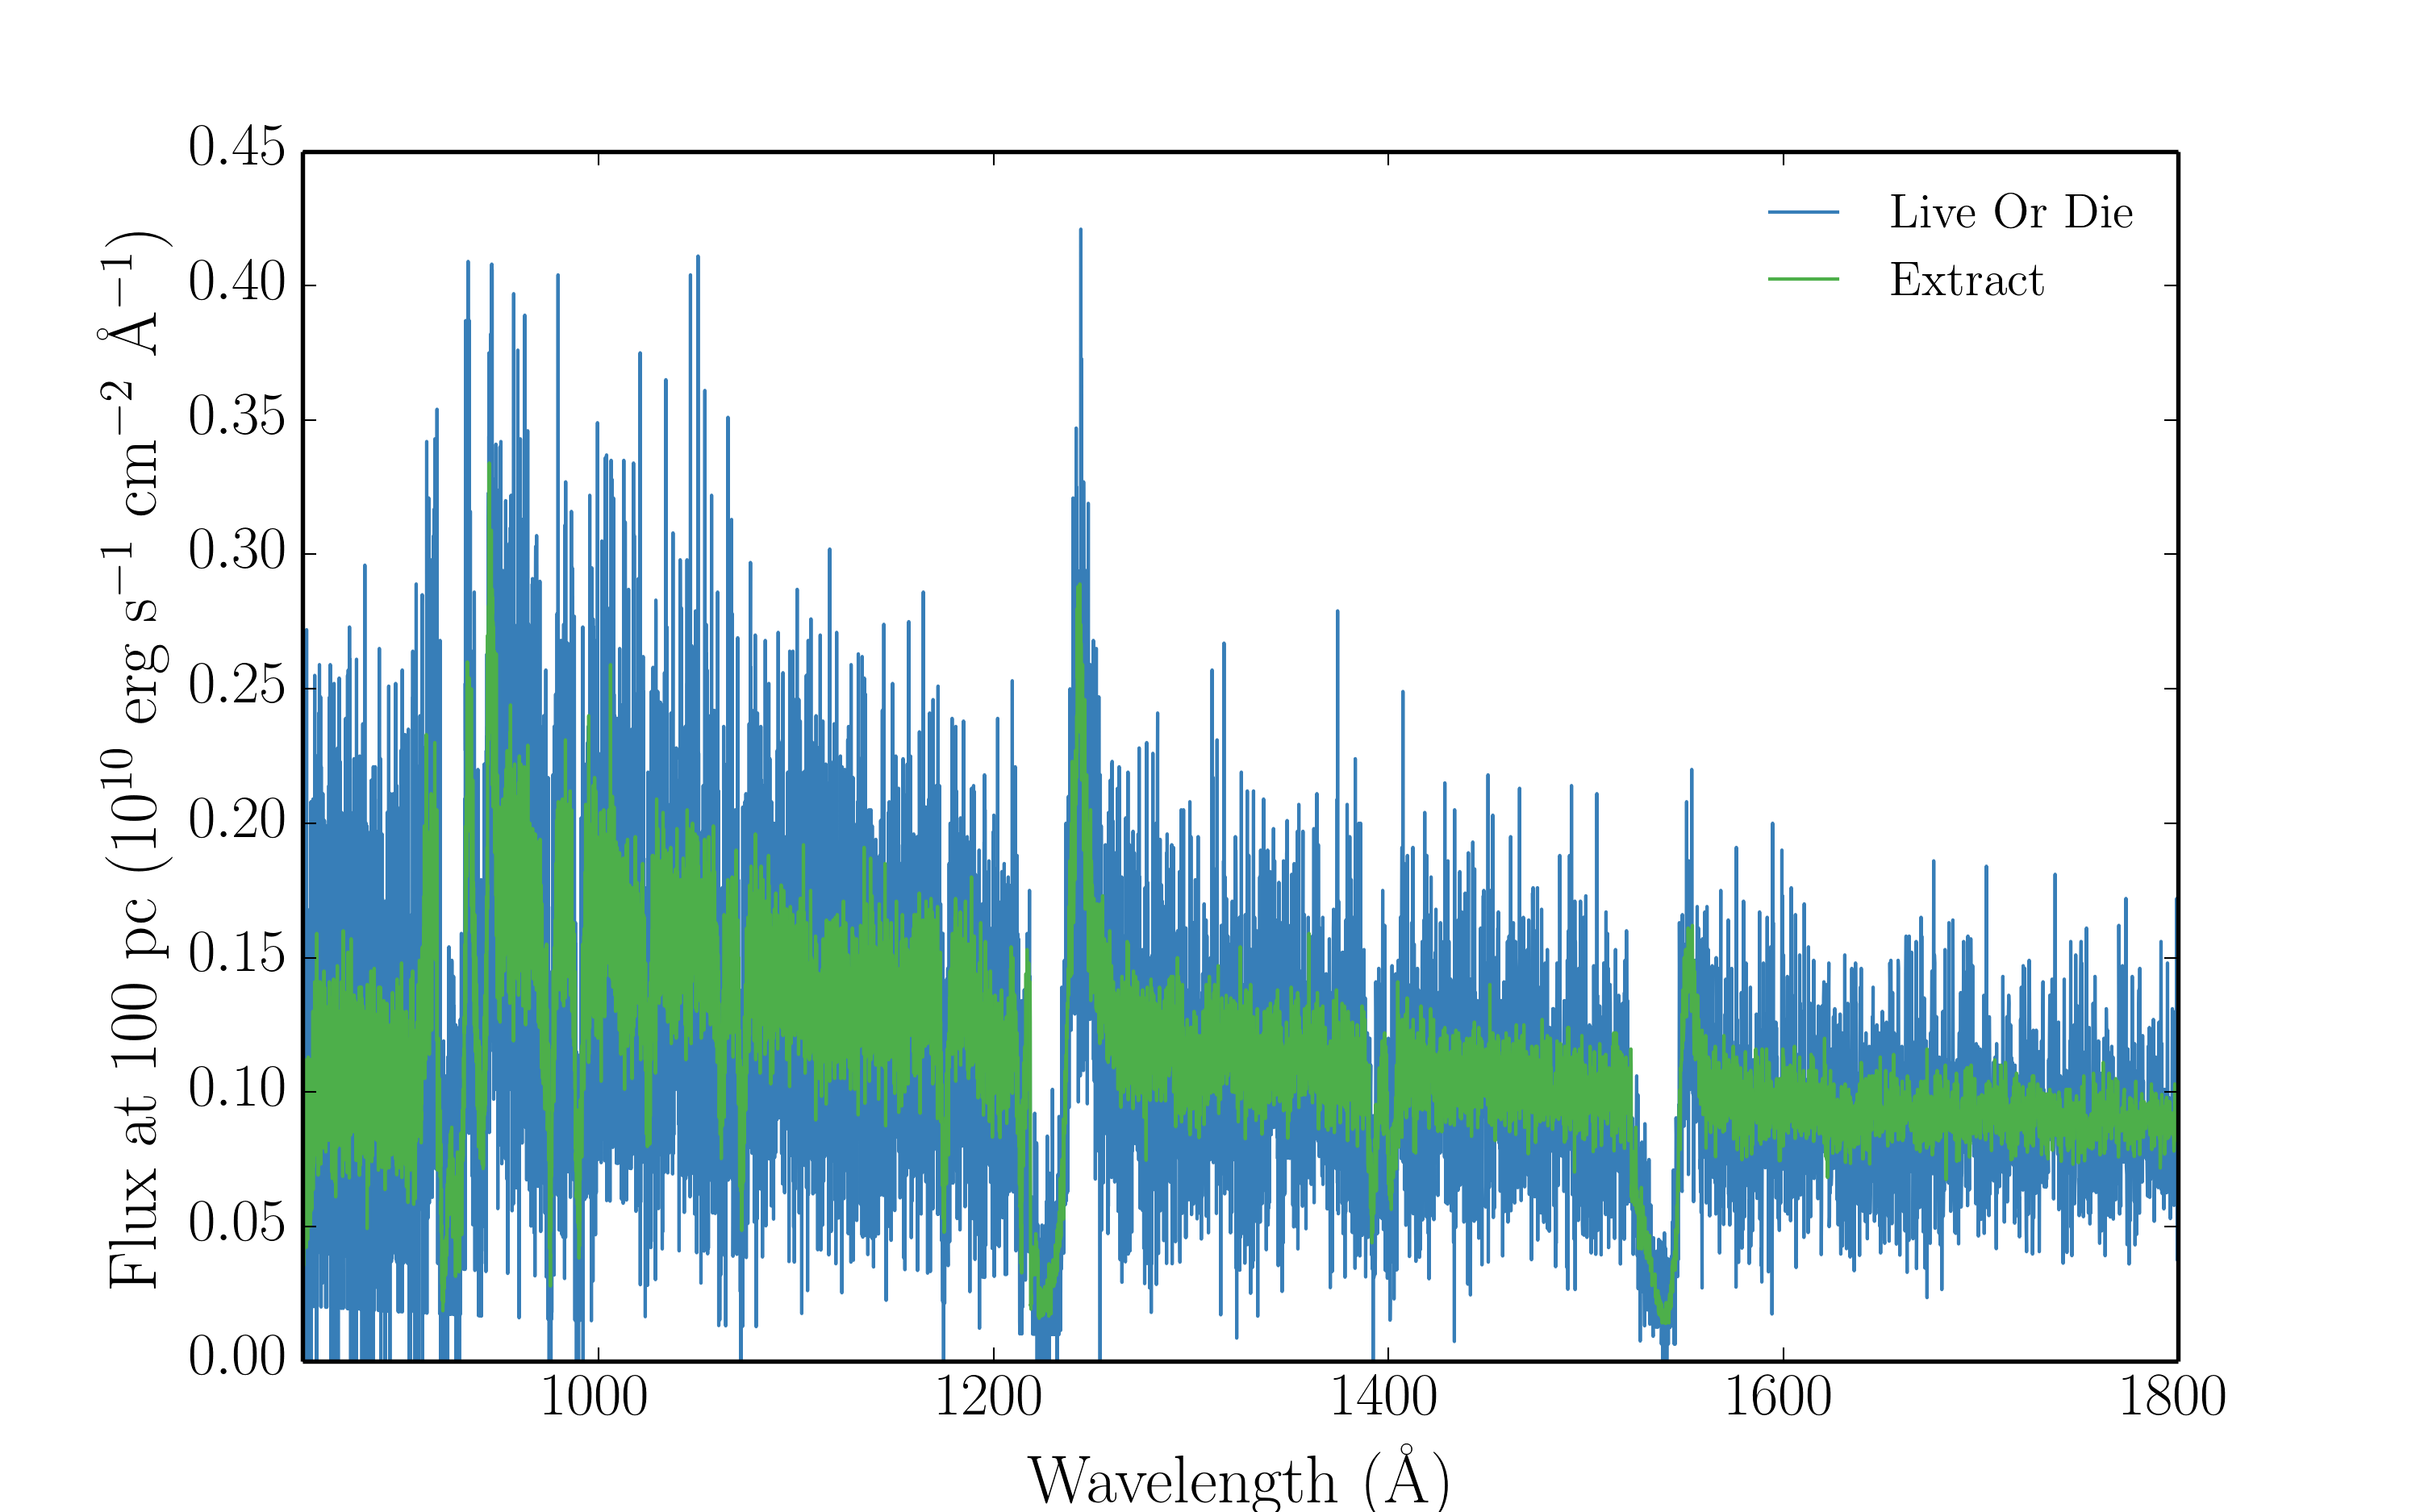
\includegraphics[width=1.0\textwidth]{figures/03-radtrans/extract_demo.png}
\caption
[A comparison of synthetic spectra produced in extract and live or die modes.]
{
A synthetic spectrum after $30$ spectral cycles with $100,000$ photons
from simple CV wind model at a $60^\circ$ viewing angle.
Spectra produced with both the extract and live or die modes
are shown. The effectiveness of the extract variance reduction technique can
be clearly seen, and we can see that the spectral shape is unaltered.
} 
\label{fig:extract_demo}
\end{figure}

\subsection{Macro-atom Emissivity Calculation}

In order to preserve the philosophy that a detailed 
spectrum is calculated in a limited wavelength regime, \py\ carries
out a macro-atom emissivity calculation before the spectral cycles.
The aim of this step is to calculate the luminosity contributed
by macro-atoms -- equivalent to the total amount of reprocessed emission -- 
in the wavelength range being considered.

This process can be very computationally intensive, especially if the wavelength regime
being simulated has very little emission from bound-free and line processes
in the wind, but the overall broad-band emissivity is high.
During the ionization cycles, the amount of energy absorbed into $k$-packets and 
every macro-atom level is recorded using MC estimators. Once 
the ionization cycles are finished, and the model has converged, these absorption
energies are split into a certain number of packets and tracked through
the macro-atom machinery until a deactivation occurs. When this happens,
the emissivity of the level the macro-atom de-activated from is incremented
if the packet lies in the requested wavelength range. If it does not, then 
the packet is thrown away. It is easy to see how what is essentially a MC rejection
method can be an inefficient way of sampling this parameter space. Fortunately,
this problem is parallelisable (see section~\ref{sec:parallel}).

Once the emissivities have been calculated, the spectral synthesis can proceed.
This is done in a different way to the ionization cycles. Photons 
are generated from the specified photon sources over the required wavelength range,
but are now also generated according to the calculated macro-atom and 
$k$-packet emissivities in each cell. These photons are `extracted' according
to the procedure outlined above.
In order to ensure that radiative equilibrium 
still holds, any photon that interacts with a macro-atom or $k$-packet is immediately 
destroyed. The photons are tracked and extracted as normal until they escape the 
simulation; resonant scatters are dealt with by a combination of
macro-atom photon production and destruction.\index{$k$-packet}

\section{Atomic Data}
\label{sec:atomic_data}
One of the big challenges in building reliable photoionization and radiative
transfer codes lies in the acquisition of accurate and complete atomic datasets.
All of the rates described so far contain a term, such as the oscillator strength 
or dimensionless collision strength, that is dependent purely on the atomic physics
associated with the transition. These quantities can be measured in laboratory experiments,
or predicted from atomic structure codes that derive the atomic physics from 
quantum theory.
\index{bound-bound collision strength}
\index{atomic data}
\index{opscillator strength}

Throughout this work, I have used very similar atomic data to that described 
by LK02 and H13. Elements included are H, He, C, N, O, Ne, Na, Mg, Al, Si, S,
Ar, Ca and Fe, although this can be easily be adapted. Solar abundances from
\cite{vernerbarthel1994} are adopted, and ionization potentials and ion
multiplicities are from \cite{verner1996}. Line information for simple-atoms 
is obtained from \citet[][$\sim5,000$ lines]{verner1996} 
and \citet[][$\sim55,000$ lines]{kurucz1995}. 
The level information for simple-atoms is constructed 
from the line lists using the technique described by \cite{lucy1999sne}.

Radiative recombination rate coefficients are taken from 
the \textsc{Chianti} database version 7.0 \citep{dere1997,landi2012}.
Ground state recombination rates from \cite{badnell2006} are adopted where available,
otherwise the code defaults to calculating recombination rates from the Milne
relation. Free-free Gaunt factors are from \cite{sutherland1998}.
\index{recombination}\index{gaunt factor!free-free}\index{Milne relation}


\subsection{Macro-atom Level and Line Data}

\index{macro-atom}\index{level population}
A 20-level model H atom was incorporated into \py\ by SDL05,
and includes line oscillator strengths from \cite{menzel1935}.
This model atom is only split according to principle quantum number $n$,
and it is thus assumed that collisions in the plasma will cause 
the $l$-subshells to be populated according to statistical weights. 
This is known as {\em $l$-mixing} and is a good approximation for hydrogen in
dense astrophysical plasmas due to the near degeneracy of the subshell 
energy levels.

In order to correctly model He recombination lines in CVs and AGN, such as the 
prominent \heiiuv\ line, I have expanded the atomic data set, so that \py\
now contains all the atomic data needed for a He macro-atom. This data was 
obtained from \textsc{Topbase}, except for some inaccurate line wavelengths
that were set to the experimental values from the National 
Institute of Standards and Technology (NIST\footnote{\url{http://www.nist.gov/}}).
He~\textsc{i} is split into $l$ and $s$ subshells so as to correctly model the
singlet and triplet lines observed in many optical spectra. He~\textsc{ii} is assumed
to be $l$-mixed, as it is hydrogenic.

For CV modelling (chapter 4), I used the full 20-level hydrogen atom, with 53 levels of 
He~\textsc{i} up to principle quantum number 10, and 10 levels of He~\textsc{ii}. 
Modelling levels close to the continuum energy can
provide a performance hit in macro-atom mode, but is necessary
when modelling recombination lines from excited 
upper levels. In quasar models (chapter 5) 
this is not as important, and the
plasma is generally more ionized. There, a 10-level hydrogen atom was used and
He~\textsc{i} was treated with only the ground state -- this simplification
had no effect on the temperature structure of the wind or emergent spectrum.

\subsection{Photoionization Cross-sections}

\index{photoionization}\index{atomic data}
Photoionization cross-sections are from \textsc{Topbase} \citep{cunto1993} and from 
\cite{vfky}. Where possible, I use \top\ photoionization cross-sections. This is because
these cross-sections are partial and represent the cross-section for a photoionization
from a given {\em level}, and so can be used to specify macro-atom 
bound-free rates to and from all configurations of the lower ion. 
I neglect photoionizations to excited configurations
of the upper ion. For simple-atoms, these cross-sections are included in the ionization
calculation, by summing over levels, but are not used for a full level populations solution.
The \top\ cross-sections have two major drawbacks in that they do not 
extend to particularly high energies and do not always contain accurate threshold
energies.

In order to improve the \top\ cross-sections, I extrapolated them to larger
energies. This was done by finding the slope, in log-log space,
of the cross-section at the maximum energy, and extrapolating to $100$~keV.
In some cases, the slope near the maximum energy was anomalous 
due to resonances or similar structure in the cross-section, or possibly
simply due to unknown problems in the \top\ calculations. These
cases were identified by eye and a $\nu^{-3}$ extrapolation
was then applied instead. 
The results of this extrapolation on the soft X-rays in an AGN model
are shown in figure~\ref{fig:xs}. Where previously there was a sharp,
unphysical edge due to the lack of high energy 
($\nu \gtrsim 10^{18}~\mathrm{Hz}$) data, 
there is now a smooth recovery to an X-ray 
power law we expect. I also manually adjusted the threshold energies in some
cases to match the more accurate values from \cite{vfky}.

\begin{figure}
\centering
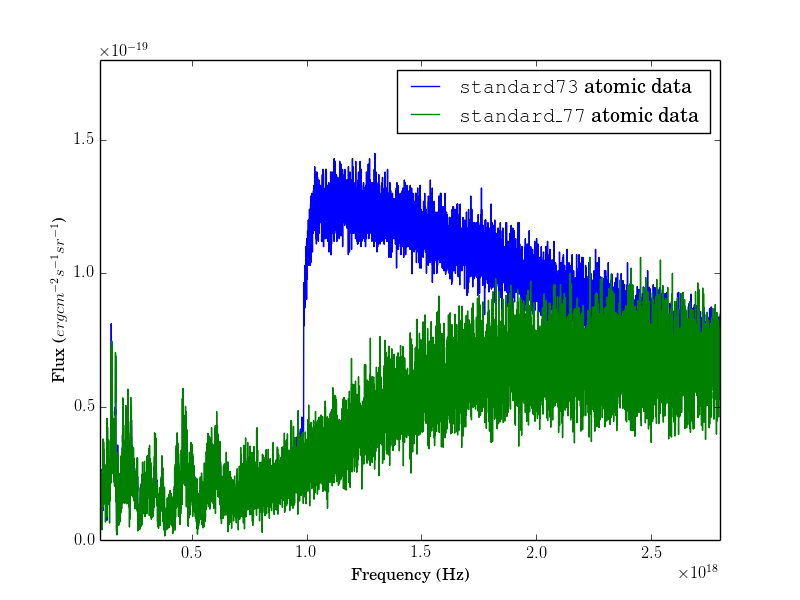
\includegraphics[width=1.0\textwidth]{figures/03-radtrans/xs.png}
\caption
[The effect of extrapolated cross-sections on the soft X-ray spectrum]
{
A comparison of the soft X-ray regime of the H13 model, with two different
datasets. standard73 is the dataset with old, unextrapolated cross-sections 
and standard77 instead includes extrapolated cross-sections as described in
the text.
}
\label{fig:xs}
\end{figure}

\section{Code Validation}
\label{sec:code_validation}

The main challenge for high performance scientific computing can be 
elegantly summarised by the \cite{ferland2002} epitaph, {\sl `Reliability in the face 
of complexity'}. I have already delved into some of the complexity in this case,
so it is important to establish whether the code is also reliable before I present
results. 

\subsection{Testing Against \cld}

\index{\cld}\index{photoionization}
\cld\ is a spectral synthesis and photoionization code used to simulate
the emergent spectrum and ionization conditions in nebulae and other plasma
environments. As a result, it uses many of the same techniques as \py\
in order to compute ionization states, level populations and heating and cooling
rates. It thus represents an excellent benchmarking tool. \py\ has been tested extensively
against \cld\ in the past; some of these successful
tests can be found in H13 and LK02.

Figs.~\ref{fig:h_cloudy} to \ref{fig:ir_cloudy} show a series of 
ionization plots with relative ion fractions plotted as a function of
ionization parameter, $U$. The ionization parameter is a useful
way to parameterise the ionization state of a plasma, and is given by
\begin{equation}
U = \frac{4\pi}{n_H c}\int_{13.6{\rm{eV}} / h}^{\infty}\frac{{J_{\nu}d\nu}}{h\nu}.
\label{eq:ip}
\end{equation}
Note the difference in form to equation~\ref{eq:xi}, as $U$ is proportionaly to
the {\em number} of ionizing photons rather than the ionizing luminosity.
In \py, the ionization parameter in a cell 
is calculated via a MC estimator, such that\index{ionization parameter}
\index{Monte Carlo!estimator}\index{photoionization}\index{ionization state}
\begin{equation}
U_{\py} = \frac{1}{c~V~n_H} \sum_i^{\mathrm{photons}} \frac{w_i \Delta s}{h \nu}.
\end{equation}
This test is designed to check that \py\ still agrees
well with \cld\ when we turn on the full macro-atom machinery.
The calculations are conducted using the same 
incident SEDs, densities and abundances, and \py\ is operated in
1D, thin shell mode to simulate an optically thin plasma and facilitate
comparison with \cld. I have shown two separate ionization modes
from \py: (i) standard mode, in which nothing is treated as a macro-atom,
and the spectral model ionization scheme of H13 is used to calculate
ion fractions; (ii) hybrid mode, in which H and He are treated as 
macro-atoms, and their level populations and ion fractions are solved
using MC estimators according to the routine
described in section~\ref{sec:matom_pops}. In both 
cases the simple-atoms have their populations calculated using the H13 scheme.
\index{\cld}

In general, the calculated fractions are in excellent agreement, with a few 
exceptions. The first problem is with He at low ionization parameters 
(see Fig.~\ref{fig:he_cloudy}), where there is a discrepancy between 
the macro-atom solution and the standard mode solution 
(the latter agrees well with \cld). This is due to 
differences in the calculated recombination rate. In macro-atom mode, 
this is done using the Milne relation for all the bound-free jumps that 
have been identified, which currently includes all transitions from the lower ion but
ignores transitions to excited states of the upper ion. By contrast, 
in standard mode, \py\ uses the recombination rates from Chianti,
which represent a weighted sum over all the possible bound-free transitions,
and are thus in some ways more complete. Neverthless, the macro-atom
scheme is self-consistent, in that all photoionization pathways have a matching 
recombination pathway, and the level populations are calculated much more
accurately. Furthermore, the models presented later generally have 
$\log U \gtrsim -2$, where the calculation
agrees well with \cld\ and standard mode.
The second problem lies in Fe, where there can be quite large differences
between \py\ and \cld. This is mainly due to Auger ionization and charge 
exchange and is currently been improved in \py, but is not included here.  
\index{\cld}\index{Auger ionization}\index{ionization state}\index{charge exchange}
\index{ionization parameter}

\begin{figure}
\centering
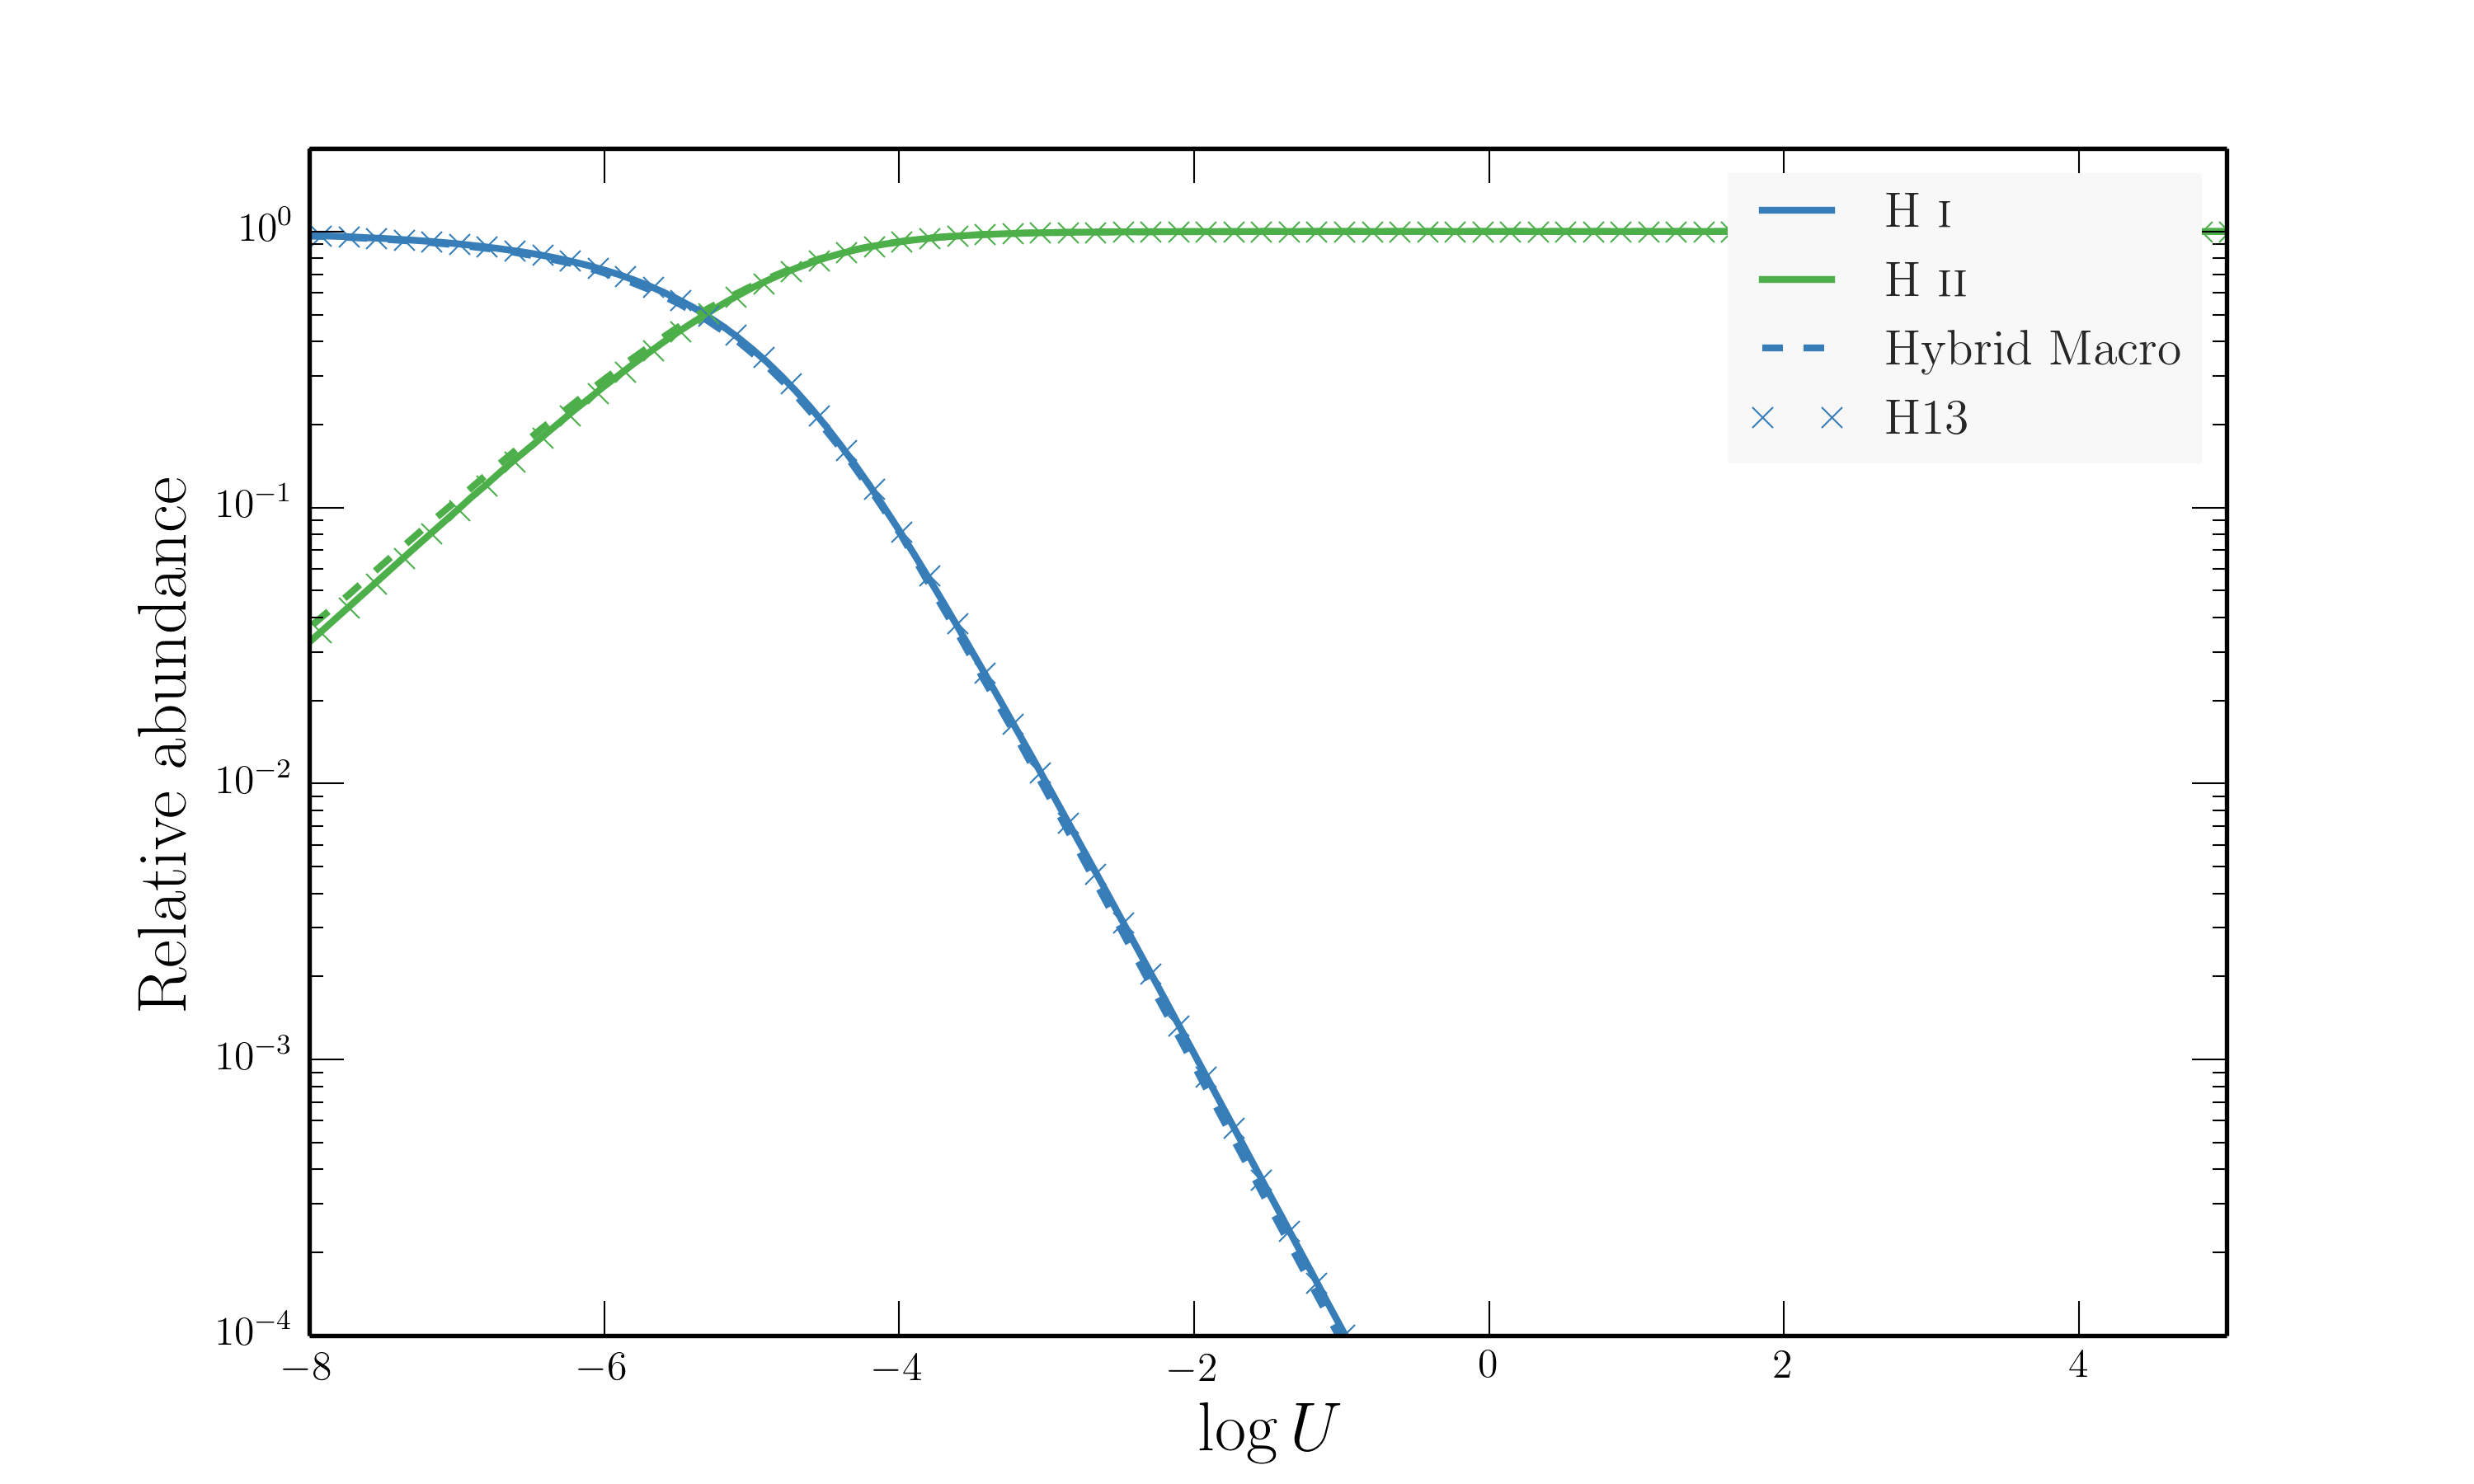
\includegraphics[width=1.0\textwidth]{figures/03-radtrans/hy_comp.png}
\caption
[Relative ion fractions for Hydrogen in \cld,\py\ in standard mode and 
\py\ in hybrid mode.]
{
Relative ion fractions as a function of ionization parameter from the
hybrid macro-atom scheme, with Hydrogen and Helium 
treated as a full macro-atom (dotted lines), compared
to both \cld\ (solid lines) and \py\ in simple-atom only mode 
(H13, crosses). The colours correspond to the different ionic stages 
and are labeled for the \cld\ case.
}
\label{fig:h_cloudy}
\end{figure}

\begin{figure}
\centering
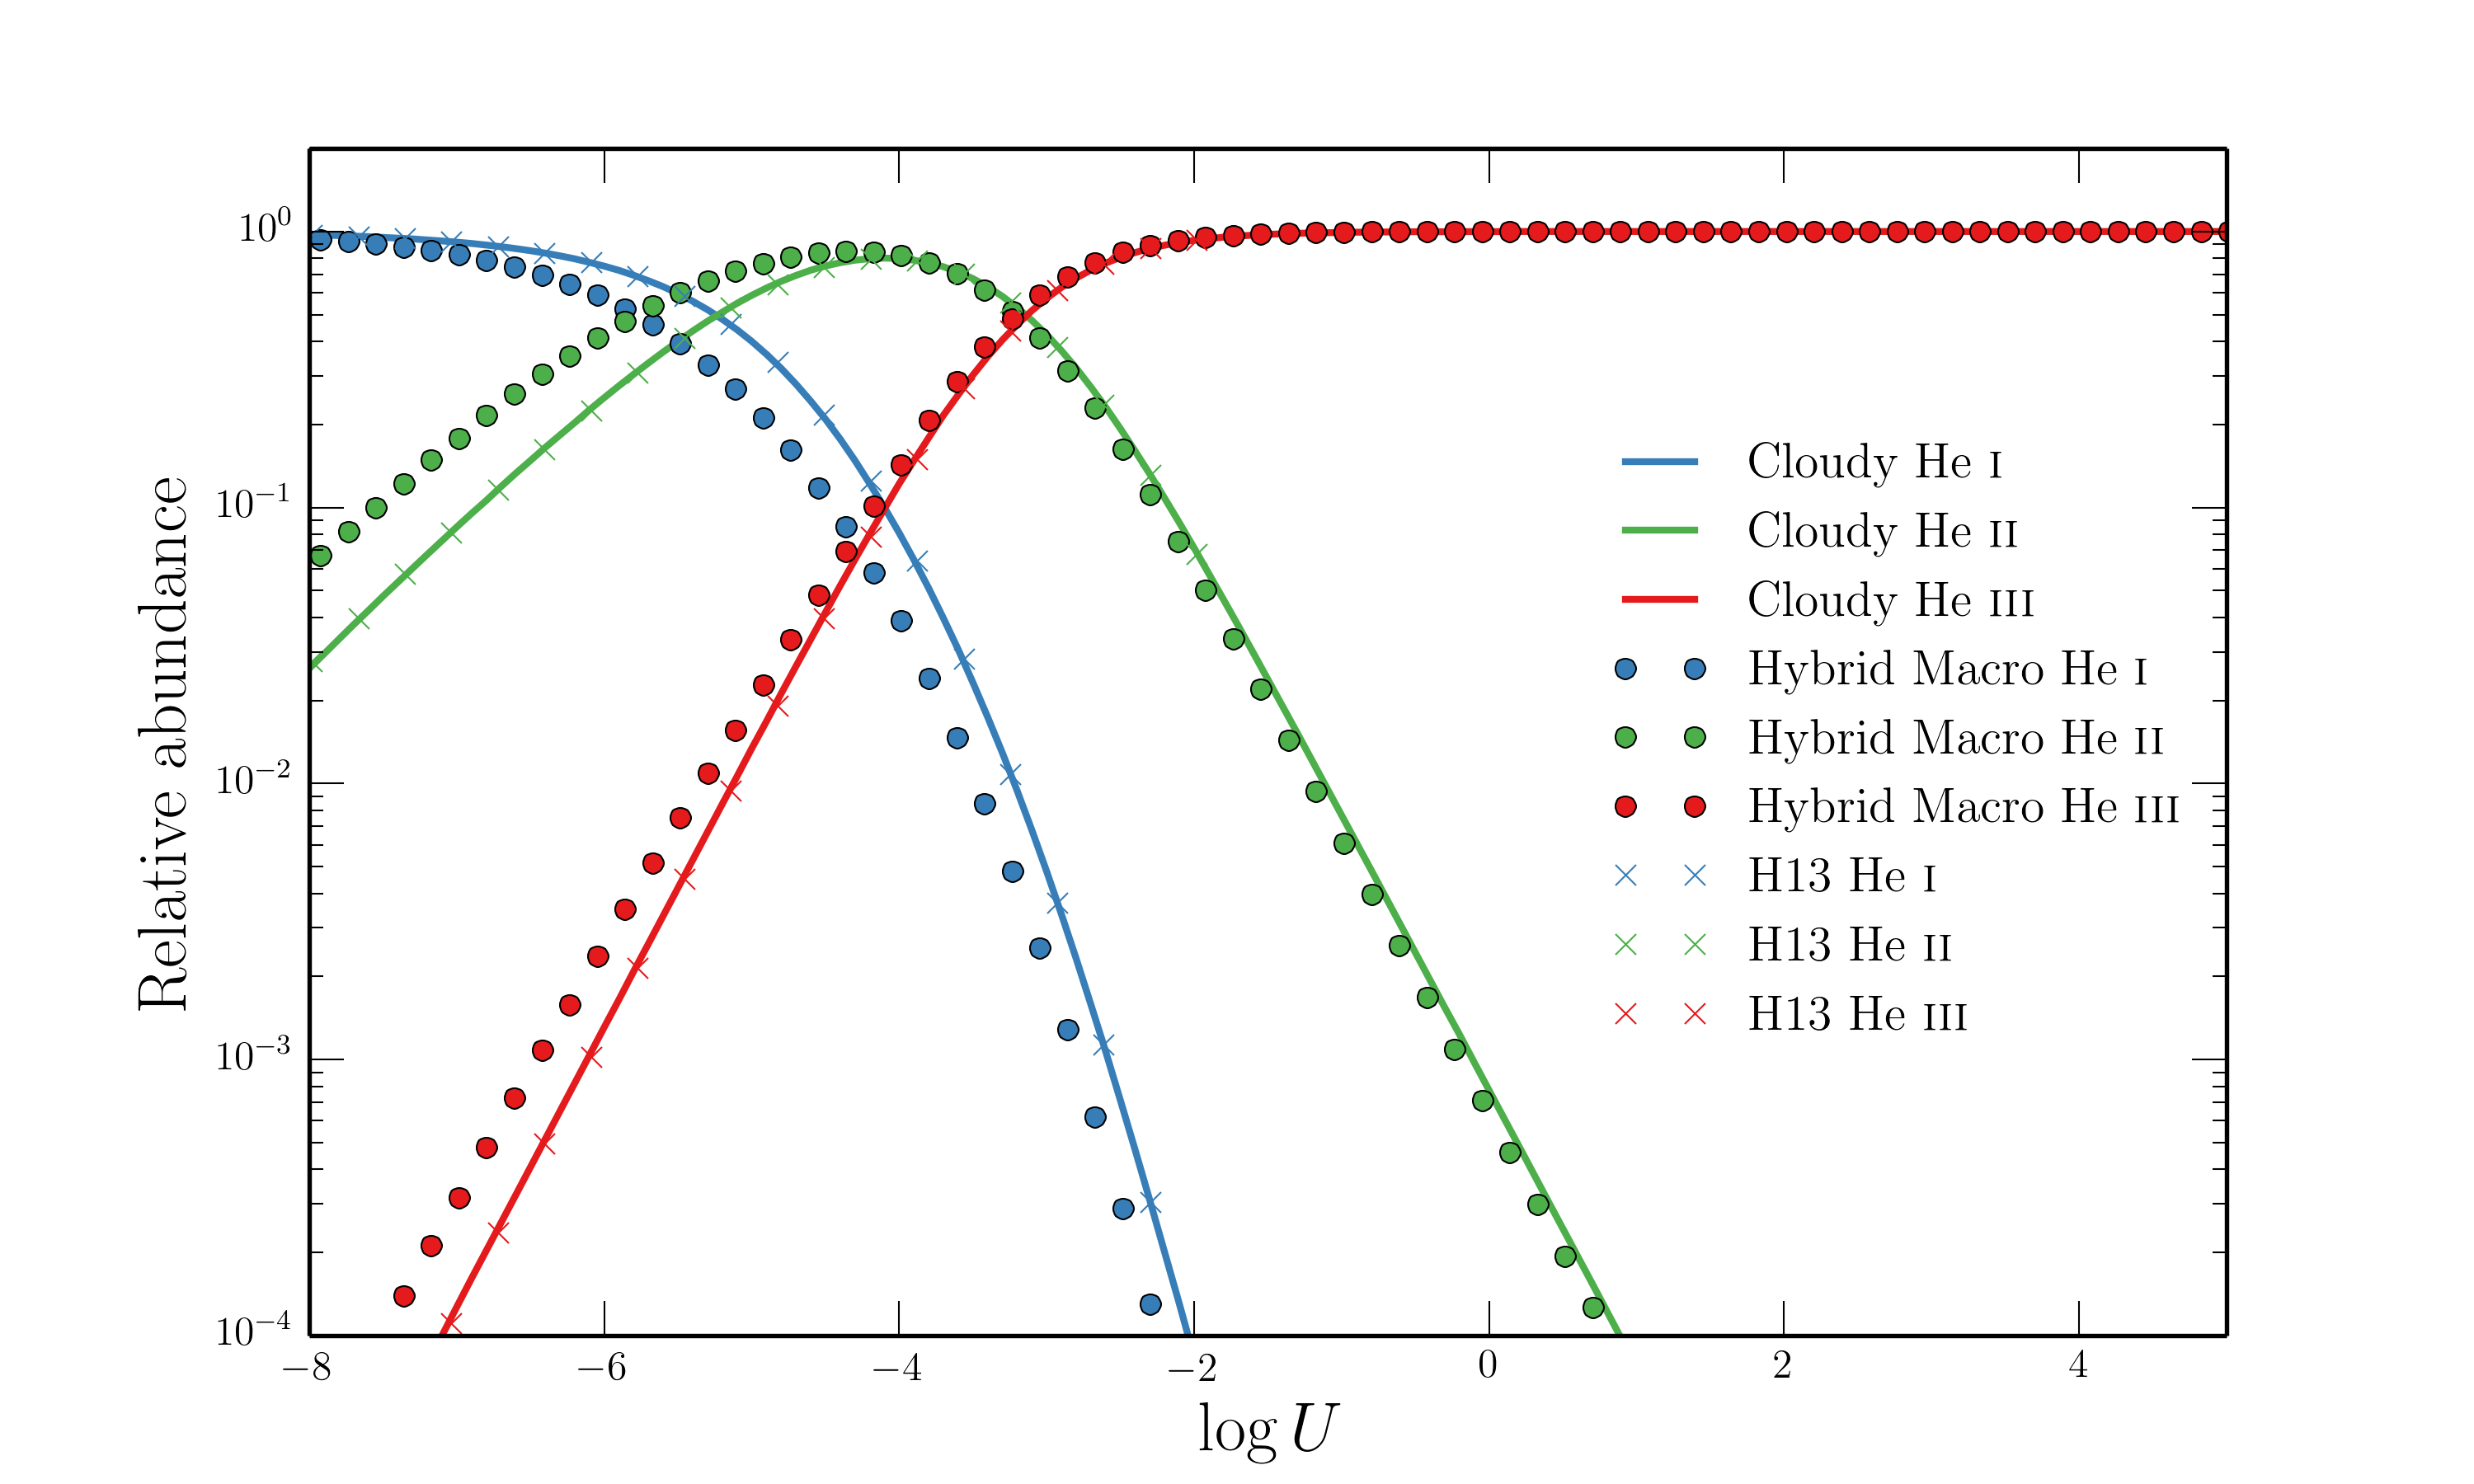
\includegraphics[width=1.0\textwidth]{figures/03-radtrans/he_comp.png}
\caption{
As figure~\ref{fig:h_cloudy}, but for Helium.
}
\label{fig:he_cloudy}
\end{figure}

\begin{figure}
\centering
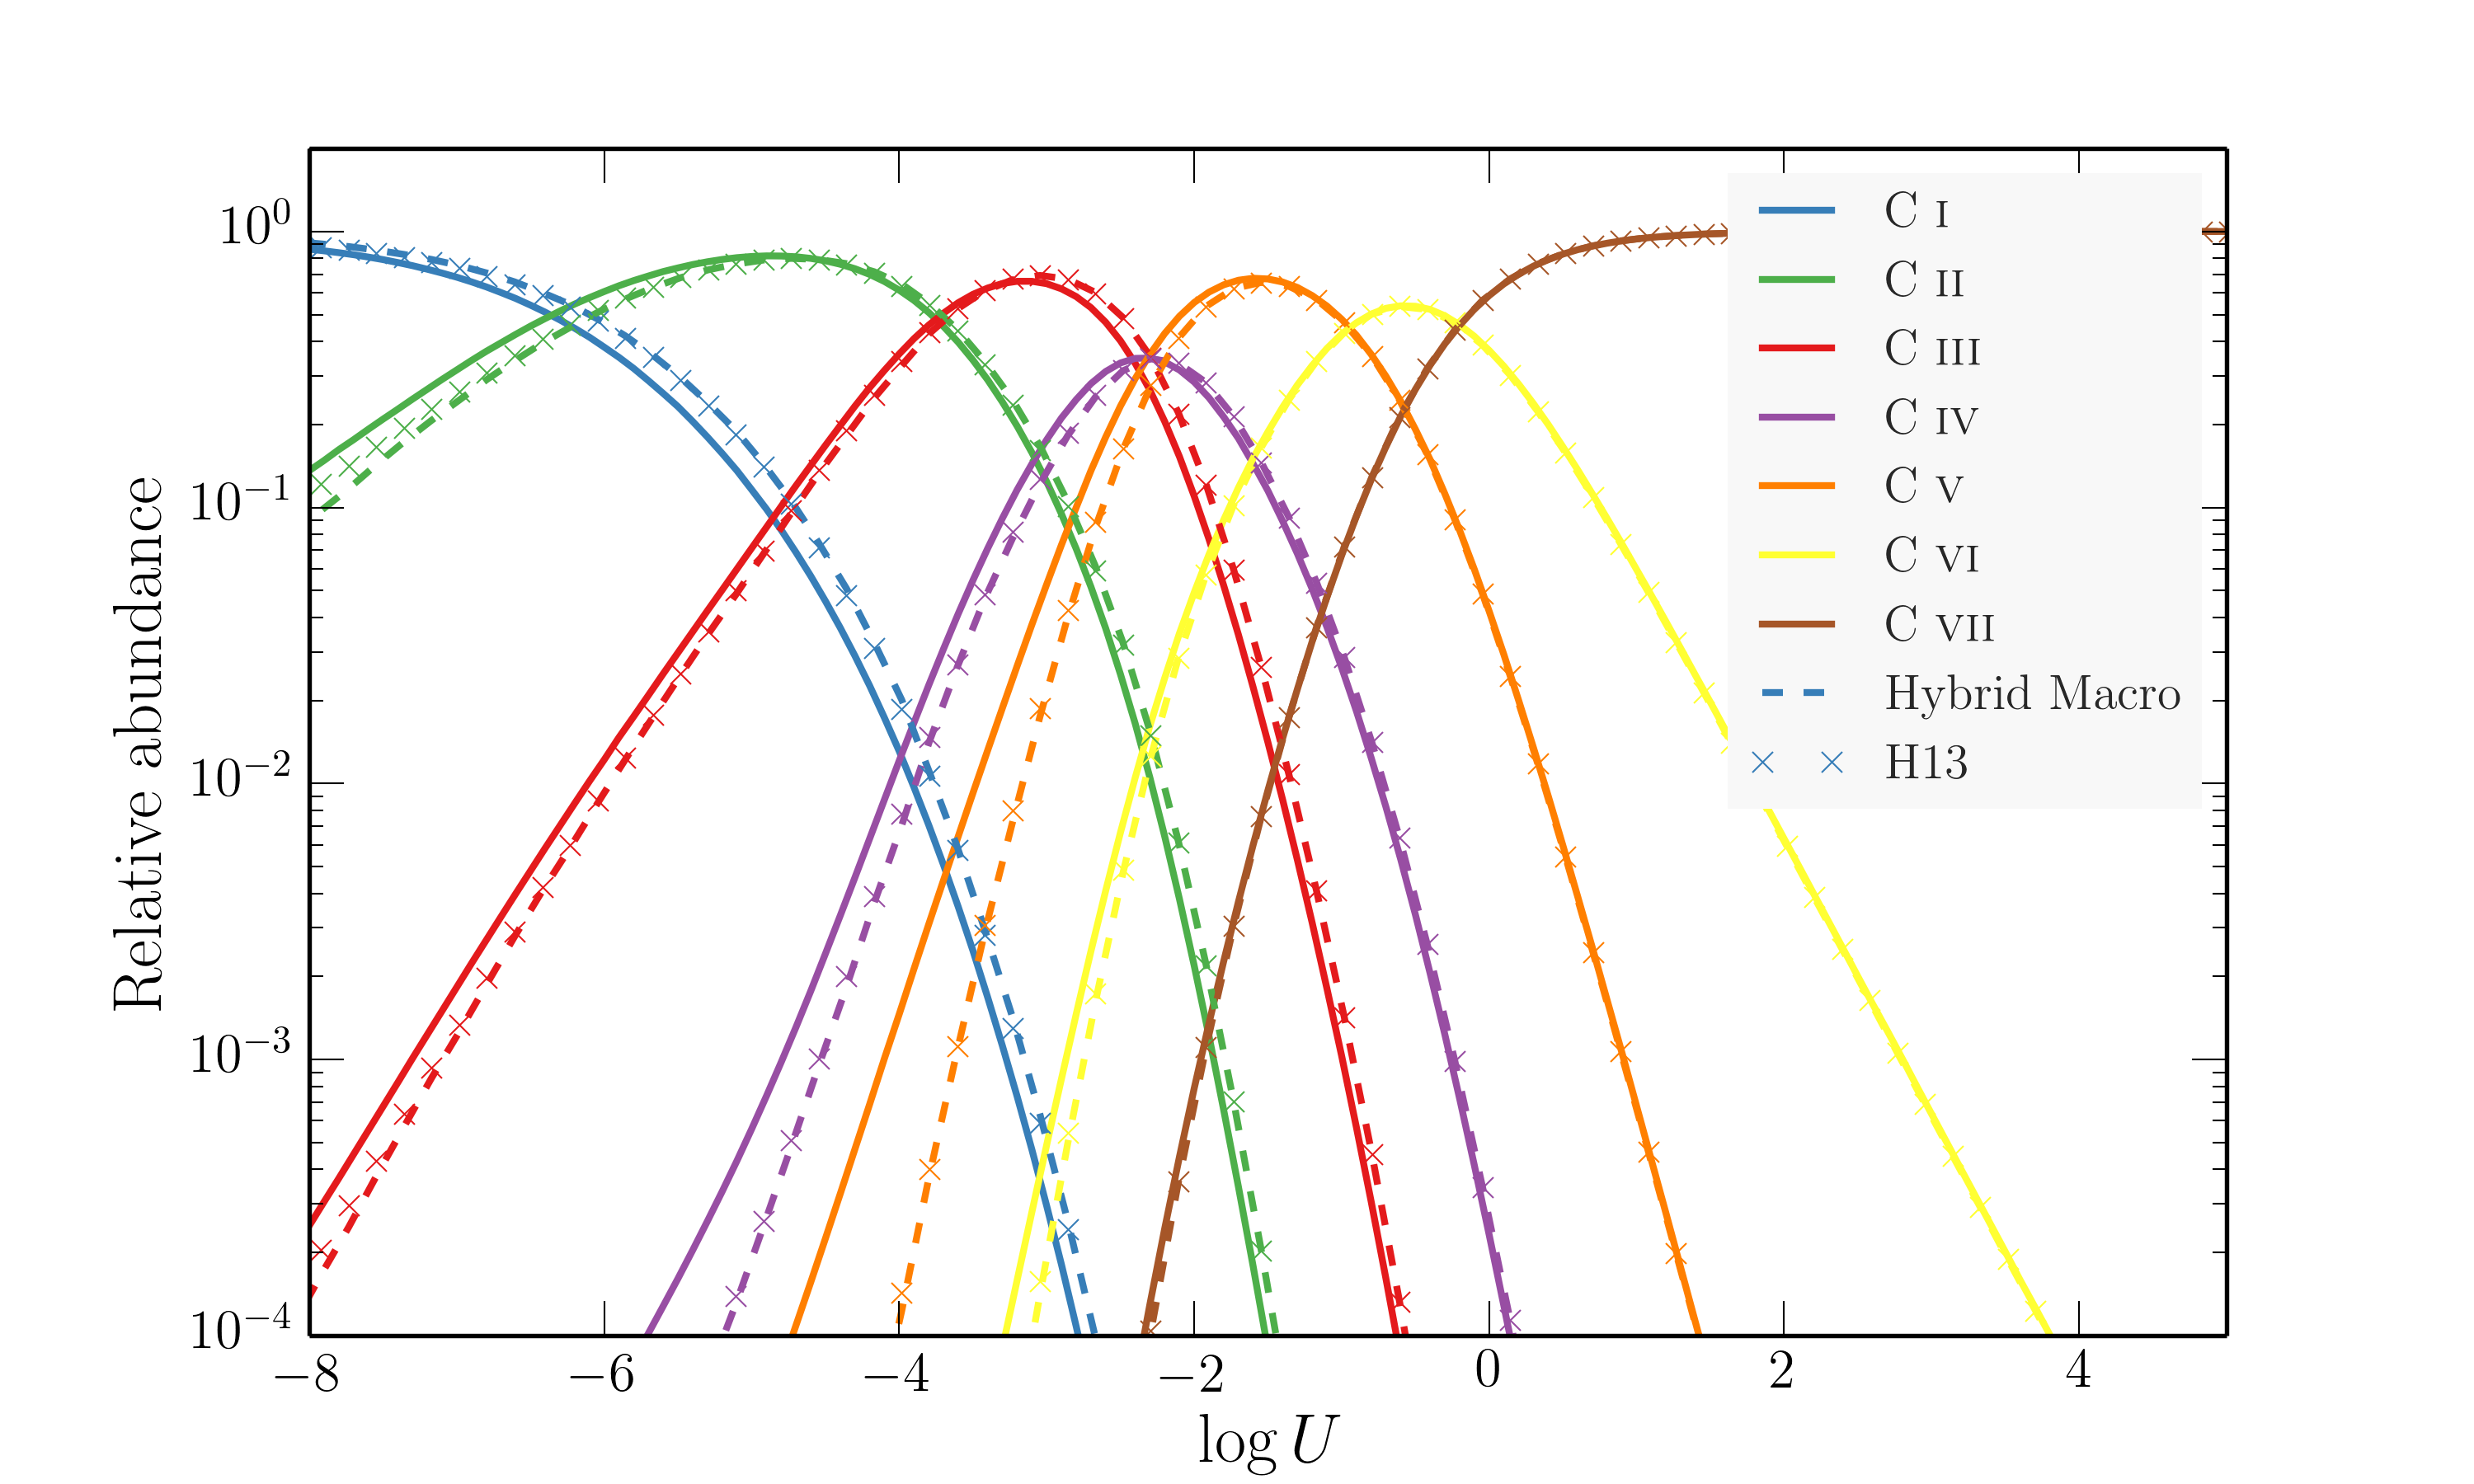
\includegraphics[width=1.0\textwidth]{figures/03-radtrans/ca_comp.png}
\caption
{
As figure~\ref{fig:h_cloudy}, but for Carbon.
}
\label{fig:c_cloudy}
\end{figure}

\begin{figure}
\centering
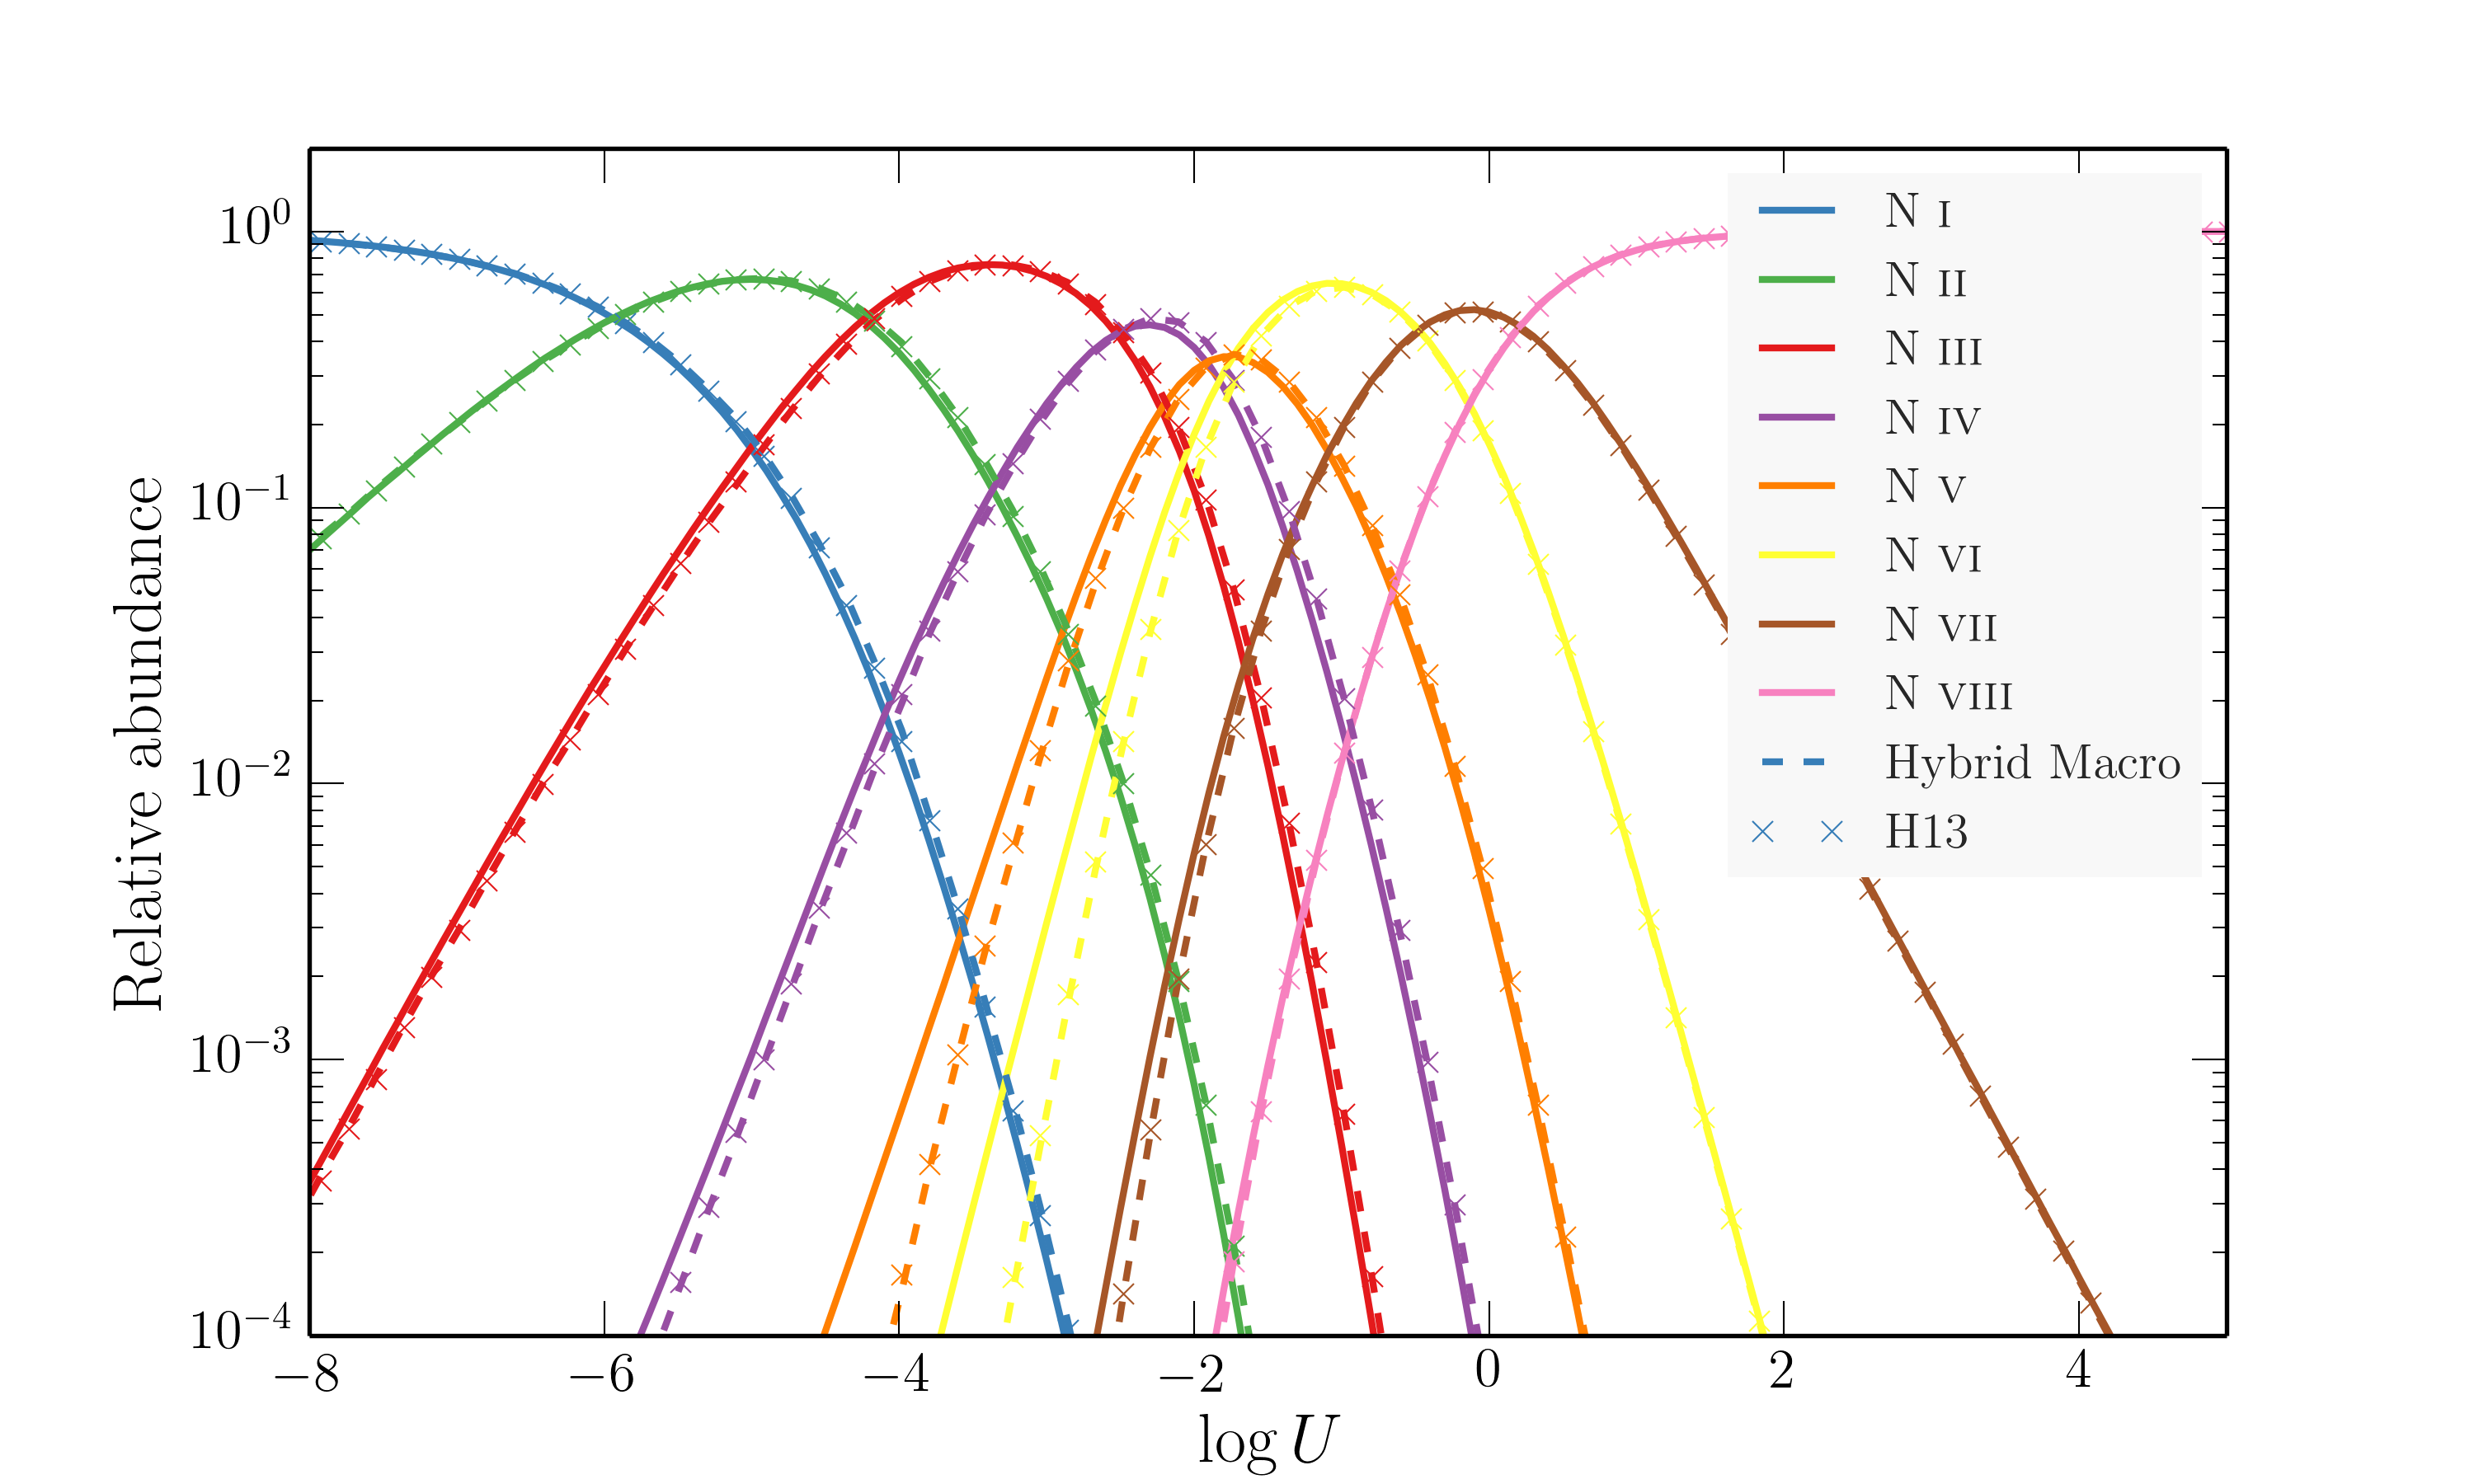
\includegraphics[width=1.0\textwidth]{figures/03-radtrans/ni_comp.png}
\caption{
As figure~\ref{fig:h_cloudy}, but for Nitrogen.
}
\label{fig:n_cloudy}
\end{figure}

\begin{figure}
\centering
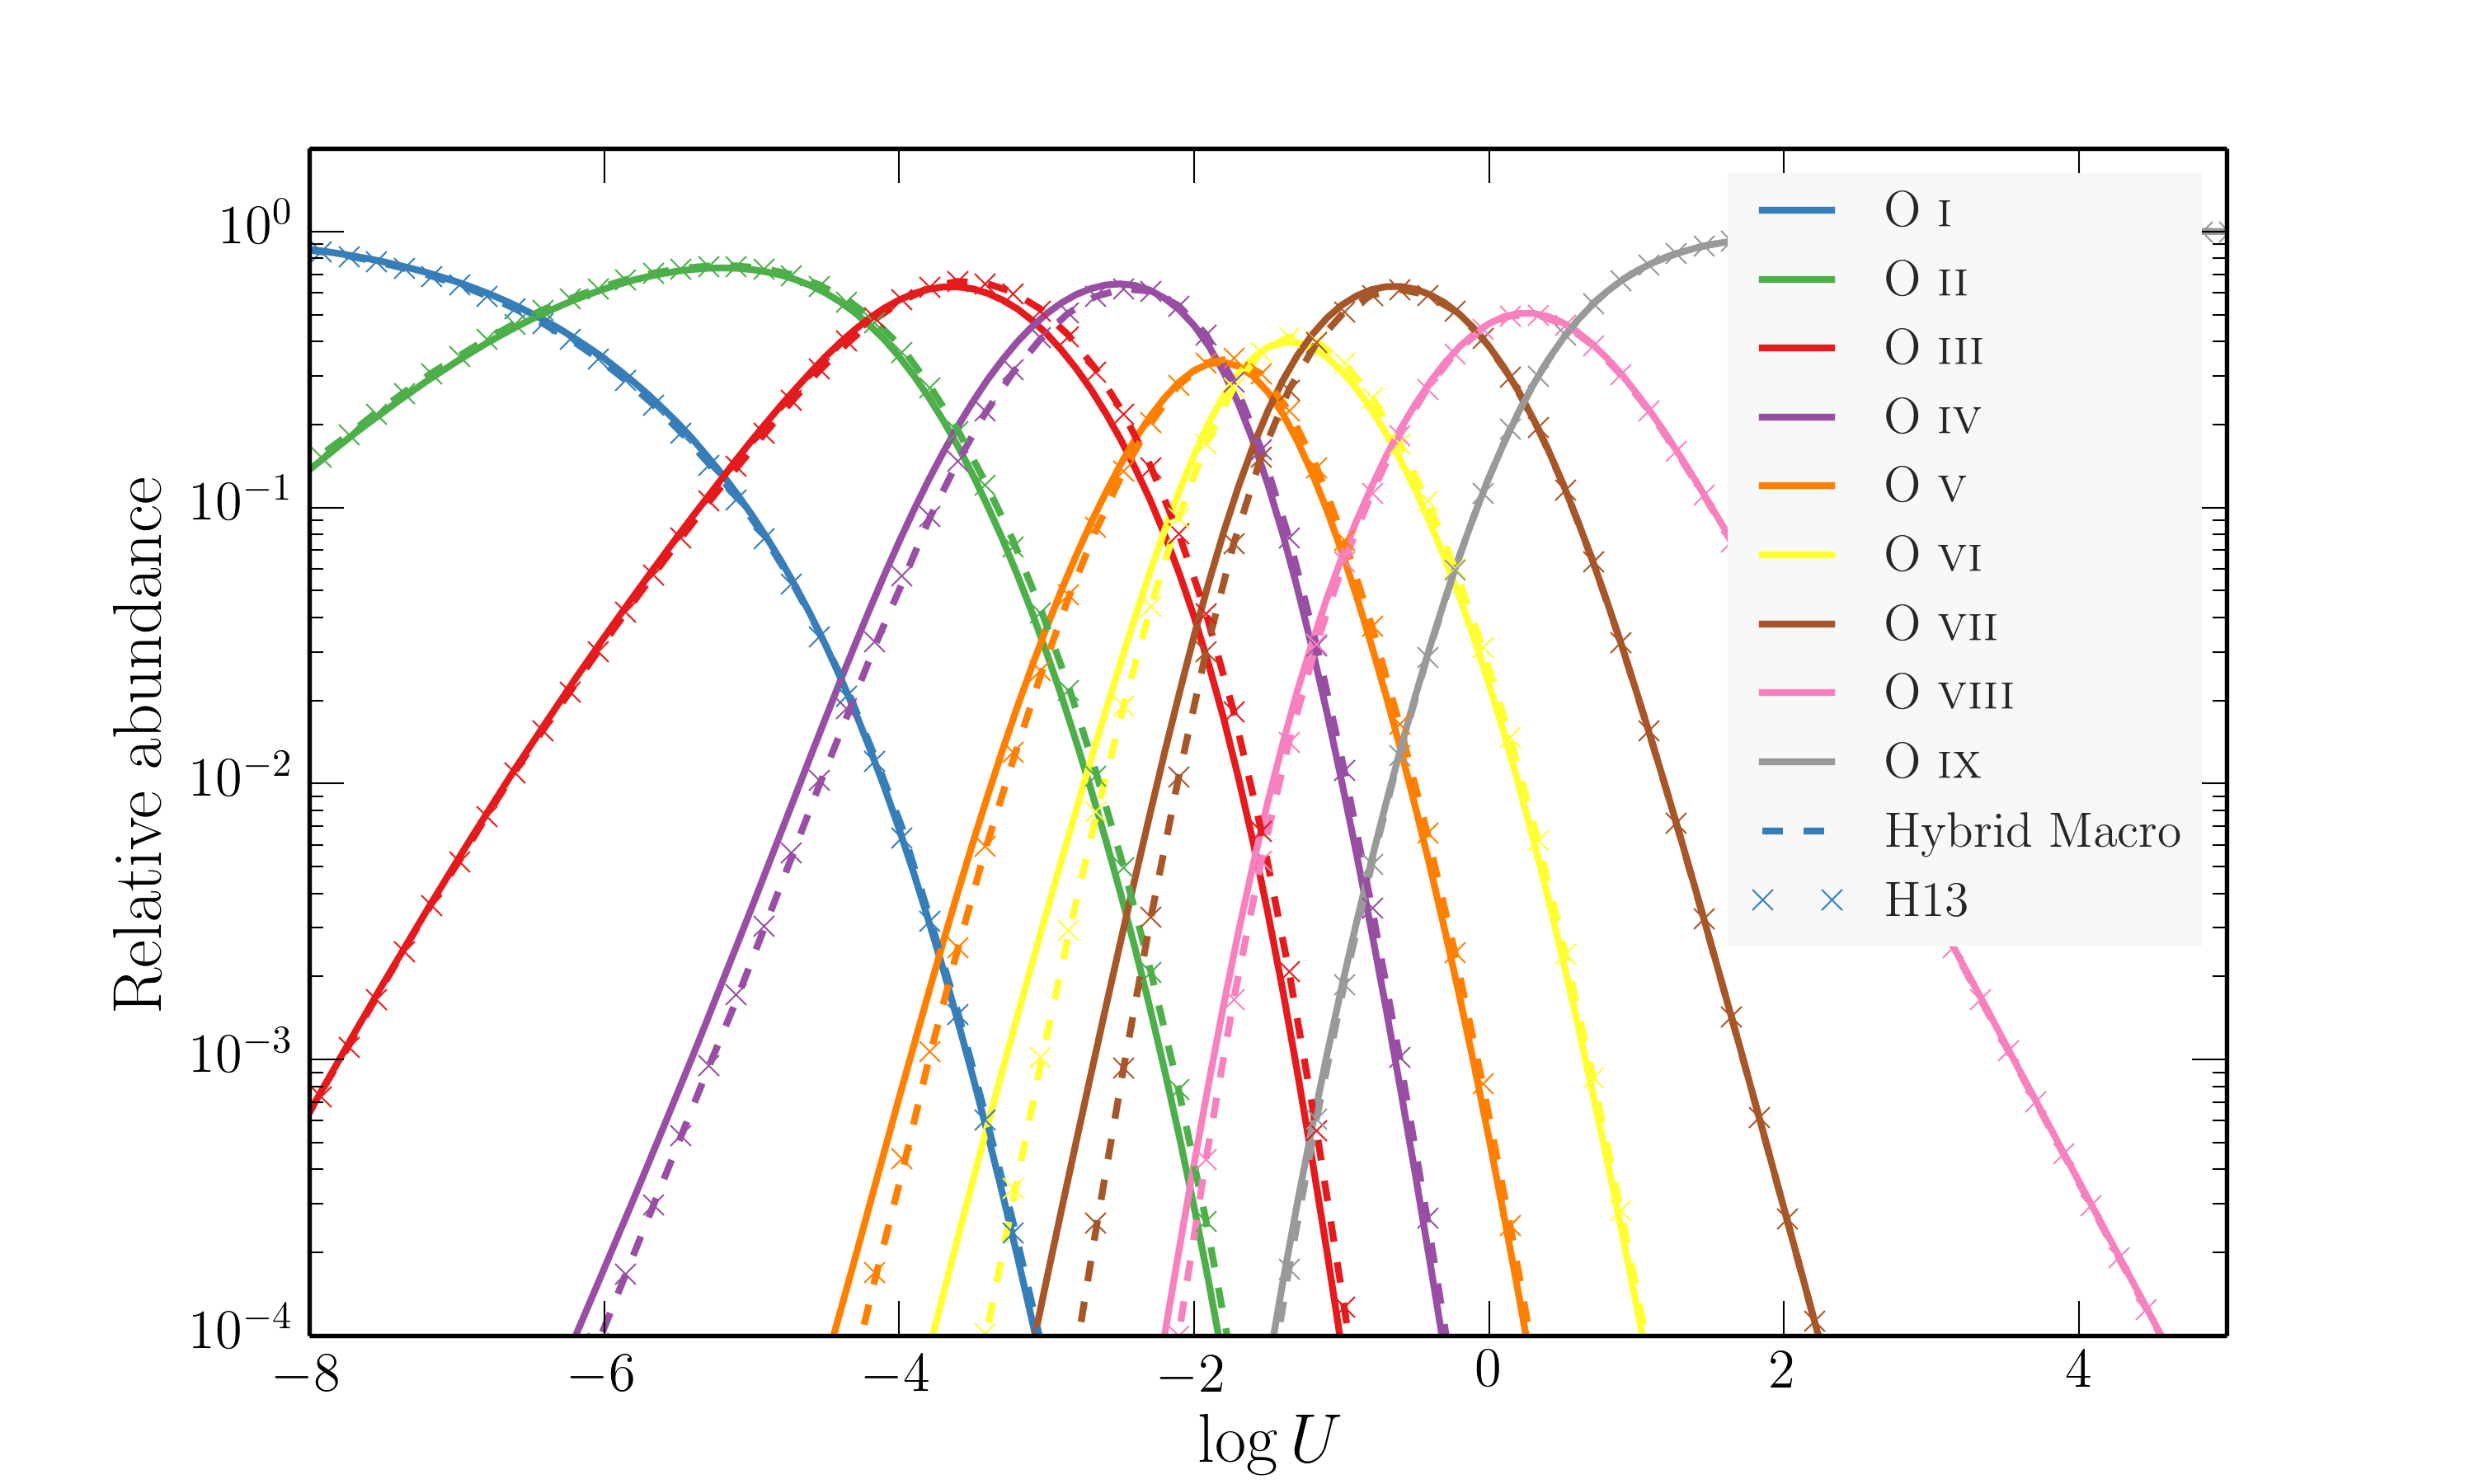
\includegraphics[width=1.0\textwidth]{figures/03-radtrans/ox_comp.png}
\caption
{
As figure~\ref{fig:h_cloudy}, but for Oxygen.
}
\label{fig:ox_cloudy}
\end{figure}

\begin{figure}
\centering
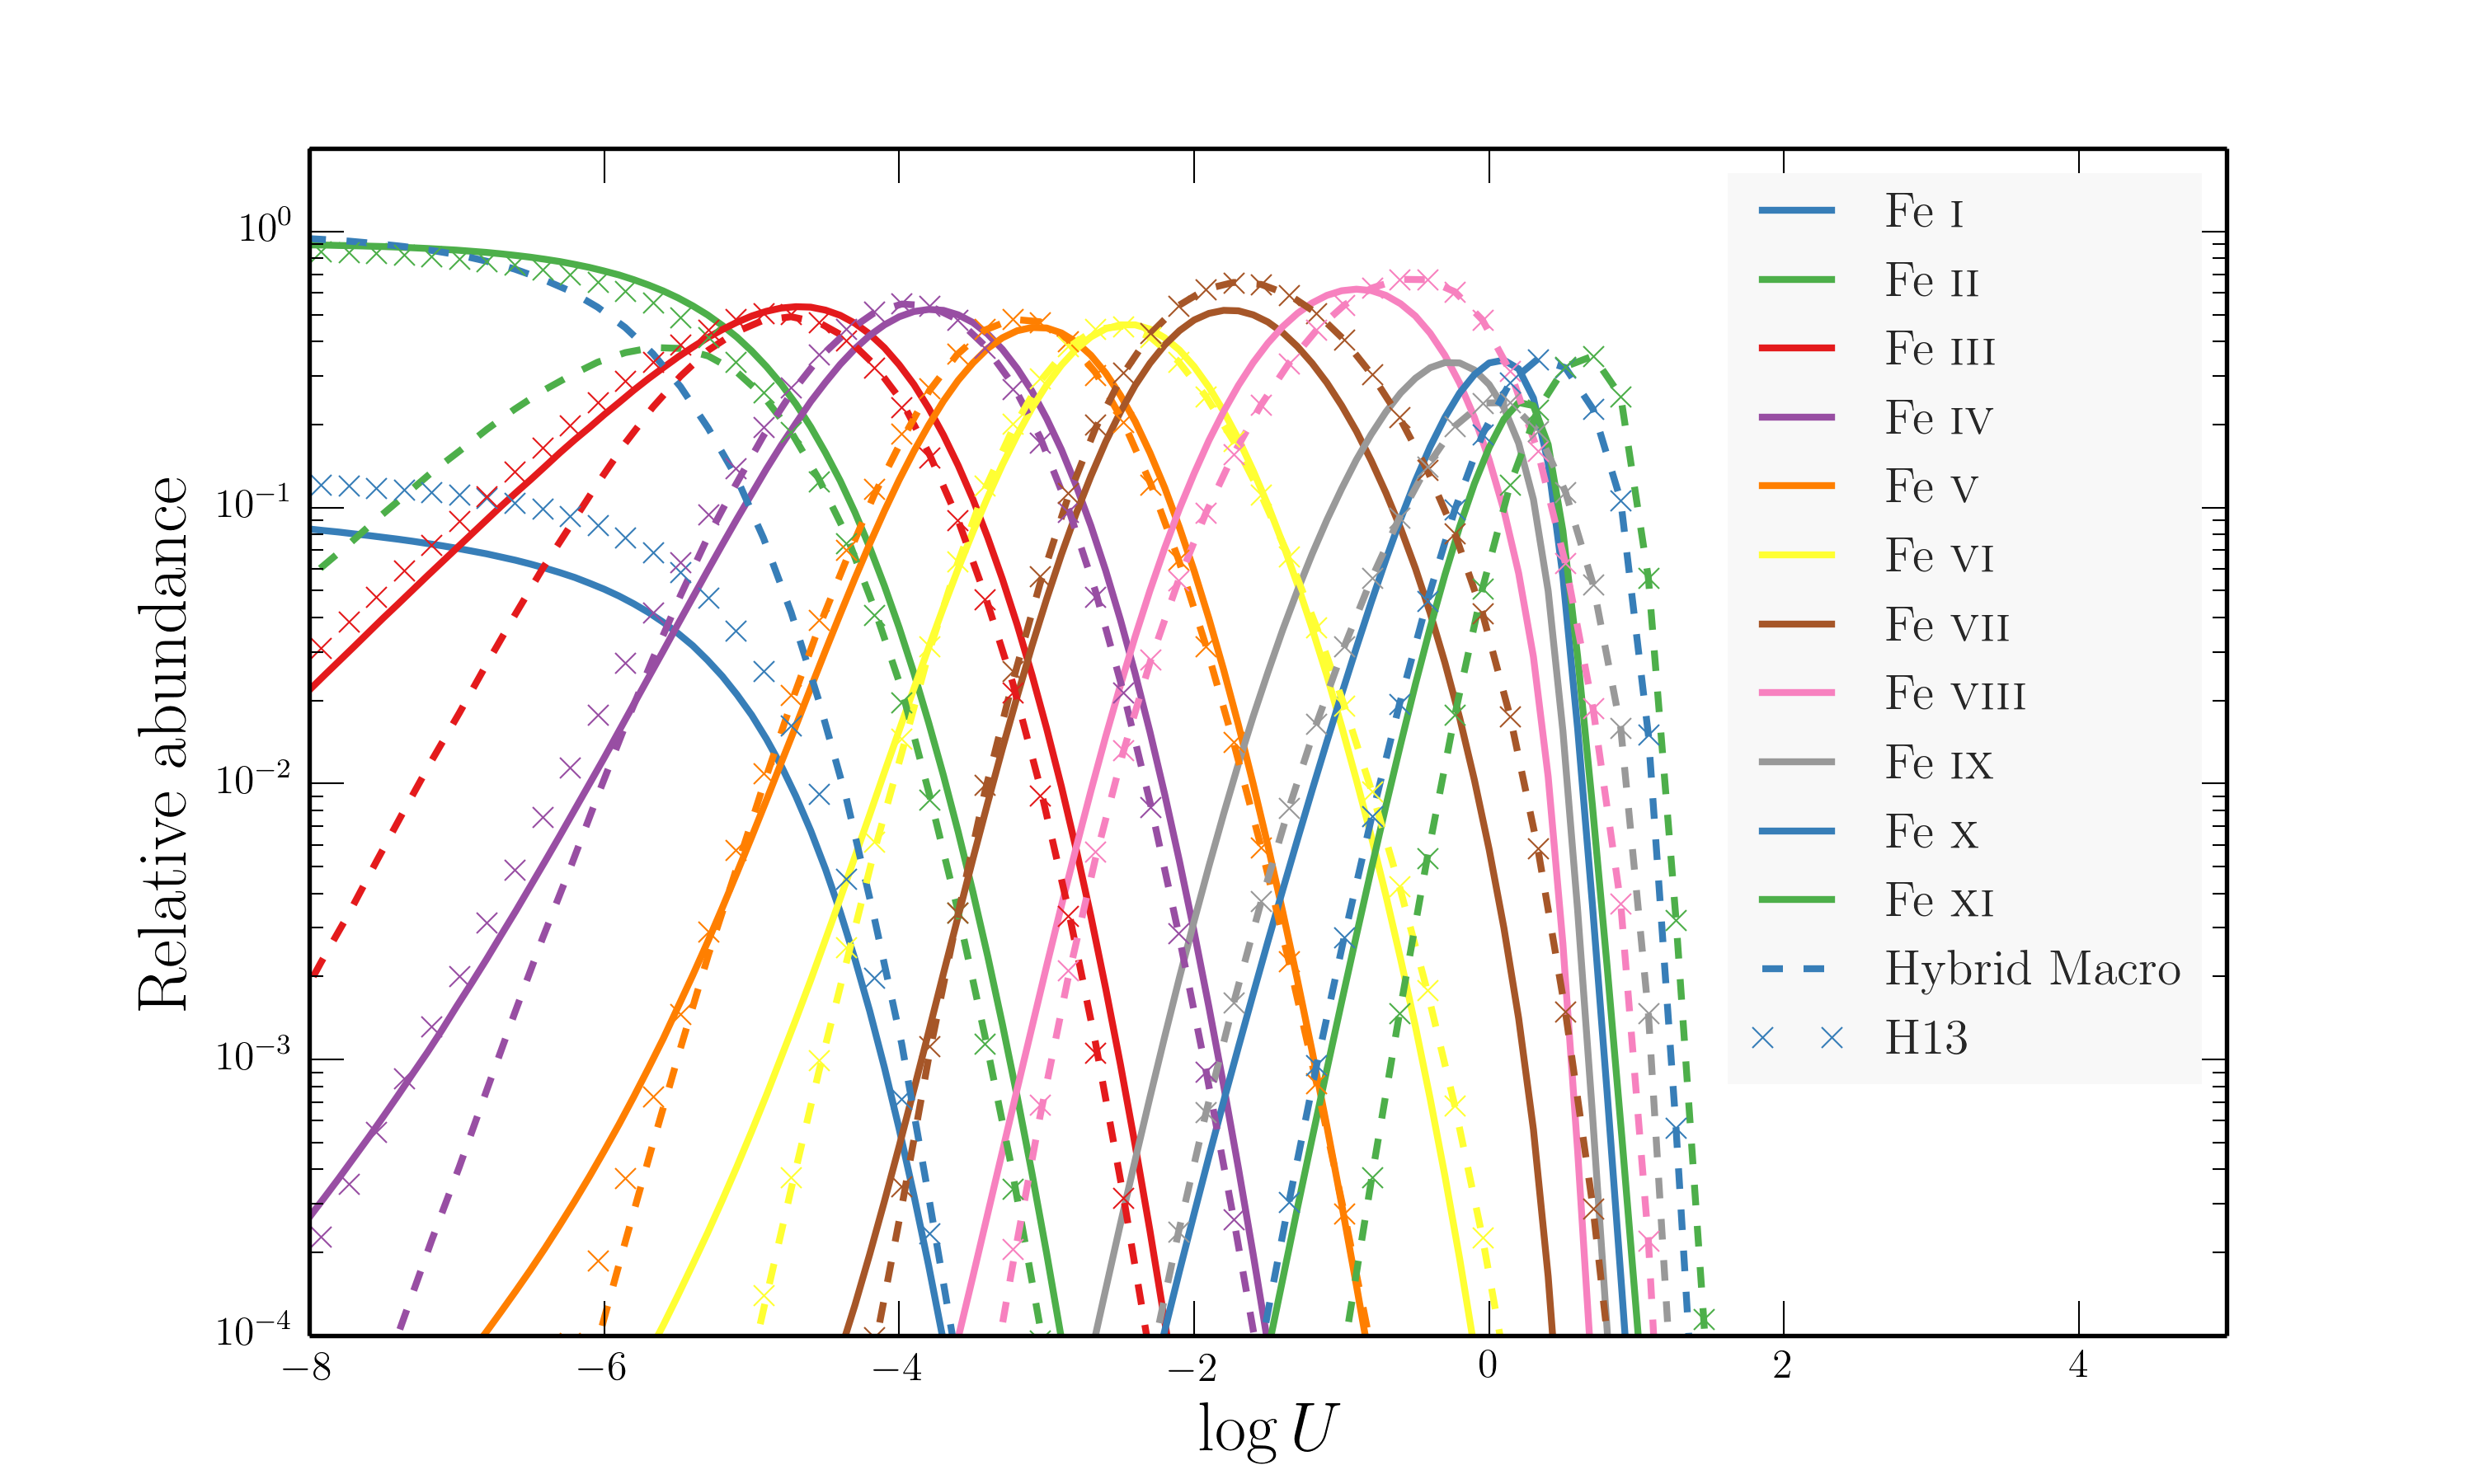
\includegraphics[width=1.0\textwidth]{figures/03-radtrans/ir_comp.png}
\caption
{
As figure~\ref{fig:h_cloudy}, but for the first 11 ionization stages of Iron.
}
\label{fig:ir_cloudy}
\end{figure}

\subsection{Macro-atom Testing Against \tar\ and Theory}

\index{\tar}\index{Supernova}
\tar\ is a 1D photoionization and radiative transfer code designed to
model supernovae in a quick and easy python package; it is described in detail by
\cite{kerzendorfsim}. Although \tar\ is simpler in terms
of geometry, it has many of the same capabilities of \py\ and 
thus makes for an excellent comparison. 

Fig.~\ref{fig:caseb_tests} shows the results of two code tests. 
In the top panel, I show a comparison of the Balmer series 
emissivities as predicted by \py\ in the l-mixed Case~B limit against the
analytical calculations by \cite{seaton1959}.\index{Case~B} 
Both calculations are calculated at $T_e=10,000$K.
Case B is an approximation commonly used in nebular astrophysics 
\citep[see e.g.][]{osterbrock} in which
one assumes that all line transitions are optically thin, except
for the \la\ transition, which is taken as optically thick.
Thus, this test comparison is carried out using a thin shell
of plasma in which the escape probabilities, $\beta_{uj}$ 
are artificially set to 1 in all transitions except \la, which
has its $\beta_{uj}$ set to 0.

The bottom panel shows a comparison of He I level populations 
(the most complex ion currently 
treated as a macro-atom) between \py\ and \tar\ models.
The calculation is conducted with physical parameters of $n_e=5.96\times10^4$~cm$^{-3}$,
$T_e=30,600$K, $T_R=43,482$K and $W=9.65\times10^{-5}$. 
Considering that the two codes use different atomic data, and that
\tar, unlike \py, includes a 
complete treatment of collisions between 
radiatively forbidden transitions, the factor of 
$<2$ agreement is encouraging. 
\index{\tar}
\begin{figure}
\centering
\includegraphics[width=1.0\textwidth]{figures/05-cvpaper/fig_caseb_tardis.eps}
\caption
[Balmer decrements in \py\ compared to Seaton (1959), and He level populations
compared to \tar.]
{
{\sl Top Panel:} `Case B' Balmer decrements computed 
with \py\ compared to analytic calculations
by Seaton (1959). Both calculations are calculated at $T_e=10,000$K.
{\sl Bottom Panel:}  a comparison of He I level populations (the most complex ion we currently 
treat as a macro-atom) between \py\ and \tar\ models. 
The calculation is conducted in thin shell mode
with physical parameters of $n_e=5.96\times10^4$~cm$^{-3}$,
$T_e=30,600$K, $T_R=43,482$K and $W=9.65\times10^{-5}$. 
}
\label{fig:caseb_tests}
\end{figure}

Fig.~\ref{fig:tardis_spec} shows a comparison 
between \tar\ and \py\ synthetic spectra from 
a simple 1D supernova model. This comparison was originally presented by
\cite{kerzendorfsim}, but I have since then discovered a bug in the Doppler shifting
routine in \py, introduced around \py\ 76, which was present in this test. 
Fixing this issue leads to slightly better agreement between the two codes. 
The model involves a full computation of the ionization state in the 
dilute blackbody mode, and, although run in 1D, it 
still tests most of the radiative transfer
machinery of the code. The spectra are in good agreement, considering
there are differences in their treatment of excitation and their atomic data.
This comparison is particular encouraging when we consider
that \cite{kerzendorfsim} also show comparisons with other supernova
codes such as \textsc{Artis} \citep{kromersim2009}, 
with similarly good agreement.

\begin{figure}
\centering
\includegraphics[width=1.0\textwidth]{figures/03-radtrans/tardispython_thesis.png}
\caption[Comparison between \tar\ and \py\ synthetic spectra from 
a simple 1D supernova model.]
{
% {\sl Credit: Kerzendorf \& Sim 2014}.
Comparison between \tar\ and \py\ synthetic spectra from 
a simple 1D supernova model. A bug in Doppler shifting of
photons was discovered around \py\ 76, meaning that the code now gives
even better agreement than presented in Kerzendorf \& Sim 2014.
% $\delta$ is an additional parameter that can be included in the ML93 equation,
% and thus the appropriate comparison here is with the $\delta=1$ case.
}
\label{fig:tardis_spec}
\end{figure}

\subsection{Testing Line Transfer Modes}
\label{sec:line_test}
The simple-atom approach has a few drawbacks. The first is that it cannot
deal well with lines in which the lower level is an excited state, such as the 
Balmer lines. This means that it is important to treat recombination lines using the 
macro-atom approach. The second is that a bound-free continuum activation, 
in normal terms a photoionization, is followed by a radiative deactivation
with the frequency chosen assuming a hydrogenic cross-section. 
This does not well represent reality, where recombining
electrons tend to do so to a variety of levels, so there is a gradual
redshifting of the radiation field. In addition, most ions are not hydrogenic. 
This problem has wider implications than
the first, as it could mean that the global ionization and temperature structure of the wind
was affected, if, for example, opacities due to elements such as C, N and O were important
in determining the ionizing radiation field.

In order to verify that this is a second order effect, 
I show a test in Fig.~\ref{fig:line_transfer} in which I compare the spectra calculated
using the indivisible 
line transfer mode against spectra calculated
using weight reduction mode (which does not make this 
approximation). The model shown is the fiducial BAL quasar model from
H13, where modelling the aborption effect on the ionizing radiation field 
properly is important due to the stratified
and self-shielding flow. As long as H and He are treated as macro-atoms, the agreement
between the modes is good, and the ionization structure in the flow is very similar.
Many of the differences in the ionization structure in the flow are actually
caused by the improved treatment of the Balmer and Lyman continua.

\begin{figure}
\centering
\includegraphics[width=1.0\textwidth]{figures/03-radtrans/line_transfer_comparison.png}
\caption
[A comparison between weight reduction and line transfer mode.]
{
A comparison between weight reduction and line transfer mode. 
The model is the H13 fiducial BALQSO model -- agreement is generally even
better for CV models. 
} 
\label{fig:line_transfer}
\end{figure}

\section{Code Maintenance and Version Control}
\label{sec:code_maintenance}

In an effort to manage the expansion of the team working on \py, I was responsible
for bringing the code under the auspices of a robust version control system.
Thanks to these efforts, the code is now hosted on GitHub at 
\url{https://github.com/agnwinds/python/}. Our team uses a Pull \& Fork model
for collaborative code development, in which major changes are made in a 
forked repository before the developer submits a `Pull request' to the main 
repository. In order to test the code, we use a combination of Travis CI build tests 
-- run for each commit to the upstream repository -- and our own test suite, which is 
run every night on a multi-core server. I have written both of these test suites.

\begin{figure}
\centering
\includegraphics[width=1.0\textwidth]{figures/03-radtrans/github1.png}
\caption
[Github commit history for \py\ from 2013-2016.]
{
Commit history from Feb 3, 2013 to Feb 29, 2016, showing the regular code development
that makes version control such a necessity to a collaborative code project. Produced
using the Github API and plotting capability.
} 
\label{fig:github}
\end{figure}

\subsection{Parallelisation} 
\label{sec:parallel}

\index{MPI}
Including macro-atoms in a simulation can have a significant impact 
on runtime, especially when simulating dense regions of plasma. 
By way of example, the CV model presented by LK02 takes approximately
118s to run one ionization cycle with $10^6$ photons. One of the macro-atom 
models presented in chapter 4 takes 5651s to complete the same task. 

Fortunately, MCRT codes are intuitively parallelisable, as is the macro-atom
emissivity calculation described above, since operations on cells or photons can
simply be divided up between processors. \py\ is parallelised using an open 
source Message Passing Interface (MPI) implementation known as 
Open MPI \citep{openmpi}. This library provides the core functions needed
in order to share out computing tasks among a series of parallel processors
with distributed memory. The parallelised elements of \py\ include
photon propagation, updating of wind ionization and temperature structure
and the calculation of macro-atom emissivities. This involves
a reasonable amount of book-keeping in that the radiation field estimators 
must be communicated between threads so as to correctly account for all
the photons that have interacted with a given cell. I have been responsible
for all of the parallelisation implemented that is
specific to the macro-atom routines.

Fig.~\ref{fig:para_times} shows the effect of parallelising a run. Due to the nature of MCRT,
it is possible to achieve significant decrease in overall 
runtime. This improvement was crucial in order to be able to run the simulation
grids used for chapters 4 and 5.


\begin{figure}
\centering
\includegraphics[width=1.0\textwidth]{figures/03-radtrans/para_times.png}
\caption
[Total runtime per cycle for an AGN run as a 
function of the number of processors.]
{
Total runtime per cycle for an AGN run as a 
function of the number of processors.
} 
\label{fig:para_times}
\end{figure}


% \section{My Contribution}

% The code and techniques described represent a large collaborative effort
% by a number of different people. It is therefore important to clearly
% identify my specific contribution to the above work.

% \begin{itemize}
% 	\item Parallelisation of the macro-atom estimators (so they are correctly communicated between threads), and the emissivity calculation described in section~??.
% 	\item Improvement of photoionization cross-sections as described in section~??.
% 	\item Incorporation of Helium macro-atom atomic data.
% 	\item Tabulation of VFKY photoionization cross-sections to avoid on the fly calculations
% 	from the fitting formulae.  
% \end{itemize}







 % Experimental Setup

\newpage
\lhead{\emph{4. The Impact of Accretion Disc Winds on the Optical Spectra of CVs}} 
%%%%%%%%%%%%%%%%%%%%%%%%%%%%%%%%%%%%%%
%
%          TITLE AND AUTHORS
%
%%%%%%%%%%%%%%%%%%%%%%%%%%%%%%%%%%%%%%%


\chapter{The Impact of Accretion Disc Winds on the Optical Spectra of Cataclysmic Variables}

{\em This chapter is based on the publication:

Matthews J. H., Knigge C., Long K. S., Sim S. A., Higginbottom N., 
`The impact of accretion disc winds on the optical spectra of 
cataclysmic variables',
2015, MNRAS, 450, 3331.}
%%%%%%%%%%%%%%%%%%%%%%%%%%%%%%%%%%%%%%
%
%          INTRODUCTION
%
%%%%%%%%%%%%%%%%%%%%%%%%%%%%%%%%%%%%%%%

\section{Introduction} 
\label{sec:intro} 

\nocite{groot2004}
\nocite{beuermann1990}
\nocite{beuermann1992}
\nocite{higginbottom2013}

\index{Monte Carlo radiative transfer}
Here, I present Monte Carlo radiative transfer simulations designed
to assess the likely impact of accretion disc winds on the
optical spectra of high-state CVs. The goal is to
test whether the disc winds that produce the UV
resonance absorption lines also naturally create significant amounts of  
optical emission. More specifically, I aim to investigate whether a 
disc wind model can reproduce the optical lines observed in CV spectra,
such as \ha, \hb, \heiiopt\ and the He~\textsc{i} lines, as well as
the \heiiuv\ emission line. I also aim to explore whether the recombination
continuum from the wind can sucessfully `fill-in' the Balmer photoabsorption
edge intrinsic to stellar or disc atmosphere spectra and to establish
if a disc wind model can produce single-peaked lines as proposed
by \citet[][hereafter referred to collectively as MC96]{MC96,MC97}.
The relevant background to this study is outlined in section~\ref{sec:cv_winds}.
\index{cataclysmic variable}\index{disc wind}

In order to carry out these simulations and effectively model the optical
spectra of CVs, I use the `macro-atom' approach described in chapter 3. 
With this method, \py\ is able to deal correctly with processes involving
excited levels, such as the recombination emission observed in CV spectra.
The prescription used to describe the wind is the biconical SV93 model described in 
section~\ref{sec:sv93_model}; a schematic for this specific application
is shown in Fig.~\ref{cartoon}. 
The remainder of this chapter is organized as follows. I begin
by describing the photon sources and input SED used in this modelling.
In section~\ref{modela}, I present spectra simulated from the benchmark 
model employed by LK02. In section~\ref{sec:modelb}, I present a revised model
optimized for the optical waveband, before summarising the
findings in section~\ref{sec:cv_conclusions}.


\subsection{Sources and Sinks of Radiation}
\label{radsources}

\begin{figure} 
\centering
\includegraphics[width=1.0\textwidth]{figures/05-cvpaper/fig2_cartoon.png}
\caption{Cartoon illustrating the geometry and kinematics of the benchmark CV wind model.}
\label{cartoon}
\end{figure} 

The net photon sources in this CV model are the accretion disc, the
WD and, in principle, a boundary layer with user-defined temperature
and luminosity. All of these radiating bodies are taken to be
optically thick, and photons striking them are assumed to be destroyed
instantaneously. The secondary star is not included as a radiation
source, but is included as an occulting body. This allows eclipses to be
modelled. Finally, emission from the wind itself is also accounted for, but
note that this assumes the outflow is in radiative equilibrium. Thus all
of the heating of the wind, as well as its emission, is ultimately
powered by the radiation field of the net photon sources in the
simulation. In the following sections, I will describe the treatment
of these system components in slightly more detail, which are also
shown in Fig.~\ref{cartoon}.

\subsubsection{Accretion disc}

\index{accretion disc}\index{accretion disc!thin disc models}
\index{blackbody}\index{stellar atmosphere}
\py\ has some flexibility when treating the accretion 
disc as a source of photons. The disc is broken down into annuli 
such that each annulus contributes an equal amount to the bolometric
luminosity. The disc is geometrically thin, but optically
thick, and I thus adopt the temperature profile of a standard
\cite{shakurasunyaev1973} $\alpha$-disc. An annulus can then
be treated either as a blackbody with the corresponding effective
temperature or as a stellar atmosphere model with the appropriate
surface gravity and effective temperature. Here, blackbodies are used
during the ionization cycles and to compute the Monte Carlo
estimators. The input SED for the ionization cycles is shown in 
Fig.~\ref{cv_model_sed}.
However, during the spectral synthesis stage of the 
simulation stellar atmosphere models are used. This produces more
realistic model spectra and allows a test of whether recombination
emission from the wind base can fill in the Balmer jump, which is
always in absorption in these models. 
The synthetic stellar atmosphere spectra are calculated with
\textsc{Synspec}\footnote{http://nova.astro.umd.edu/Synspec43/synspec.html}
from either Kurucz \citep{kurucz1991} atmospheres (for $T_{\mathrm{eff}} \leq
50,000$~K) or from \textsc{TLUSTY} \citep{tlusty} models (for $T_{\mathrm{eff}} > 50,000$~K). 
\index{accretion disc}\index{stellar atmosphere}\index{\textsc{TLUSTY}}
\index{Balmer edge}

\begin{figure} 
\centering
\includegraphics[width=0.8\textwidth]{figures/05-cvpaper/sed.png}
\caption[The spectral energy distribution of the 
accretion disc and white dwarf used in the ionization cycles for
the CV modelling.]{The spectral energy distribution of the 
accretion disc and white dwarf used in the ionization cycles for
the CV modelling. The important ionization edges for
hydrogen and helium are marked.}
\label{cv_model_sed}
\end{figure} 

\subsubsection{White Dwarf}

The WD at the center of the disc is always present as a spherical occulting
body with radius $R_{WD}$ in \py\ CV models, but it can also be included
as a source of radiation. In the models presented here,the
WD is treated as a blackbody radiator with temperature $T_{WD}$ and luminosity
$L_{WD} = 4\pi R_{WD}^2 \sigma T_{WD}^4$.\index{white dwarf}
\index{blackbody}

\subsubsection{Boundary Layer}

It is possible to include radiation from a boundary layer (BL) between
the disc and the WD. In \py, the BL is described as
a blackbody with a user-specified effective temperature and
luminosity. The models presented here initially follow LK02 in setting
the BL luminosity to zero, partly as the temperature, luminosity, and even
existence of a BL in CVs with strong winds is not certain \citep{hoaredrew1993}.
However, I have confirmed that the addition 
of an isotropic BL with $L_{BL} = 0.5 L_{\mathrm{acc}}$ and temperatures in 
the range $80~{\rm kK} \leq T_{BL} \leq 200~{\rm kK}$ would not change 
any of the main conclusions here. 
The influence of the BL on the heating and cooling balance
in the wind, as well as the emergent spectrum, is briefly discussed in
section~\ref{sec:coll_bl}.
\index{boundary layer}\index{blackbody}


\subsubsection{Secondary Star}

The donor star is included in the system as a pure radiation sink, 
i.e. it does not emit photons, but absorbs any photons that strike its
surface. The secondary is assumed to be Roche-lobe filling, so its
shape and relative size are defined by setting the mass ratio of the system, 
$q_M = M_2/M_{WD}$. The inclusion of the donor star as an occulting body
allows eclipses of the disc and the wind to be modelled. For this
purpose, I assume a circular orbit with a semi-major axis $a$ and 
specify orbital phase such that $\Phi_{\mathrm{orb}} = 0$ is the
inferior conjunction of the secondary (i.e. mid-eclipse for $i \simeq
90^\circ$).\index{Roche-lobe}




%%%%%%%%%%%%%%%%%%%%%%%%%%%%%%%%%%%%%%
%
%          BENCHMARK MODEL
%
%%%%%%%%%%%%%%%%%%%%%%%%%%%%%%%%%%%%%%%


\begin{table}
\centering
\begin{tabular}{p{2cm}p{2cm}p{2cm}}
%\multicolumn{2}{l}{Model Parameters}  \\
%%Model Parameters \\
\hline Parameter 	&	 Model A  & Model B \\ 
\hline \hline 
$M_{WD}$ 	 &	 $0.8~M_{\odot}$  &     \\ 
$R_{WD}$ 	 &	 $7\times10^{8}$~cm  & \\ 
$T_{WD}$ 	 &	 $40,000$~K        &  \\
$M_{2}$ 	& -&	 $0.6~M_{\odot}$   \\ 
$q_M$ 	&- &	 $0.75$   \\ 
$P_{\mathrm{orb}}$ 	&- &	 $5.57$~hr   \\ 
$a$ 	& -&	 $194.4~R_{WD}$   \\ 
$R_2$   &   -  &	 $69.0~R_{WD}$  \\ 
$\dot{M}_{\mathrm{acc}}$ 	 &	 $10^{-8}~M_{\odot}\mathrm{yr}^{-1}$  &\\ 
$\dot{M}_W$  &	$10^{-9}~M_{\odot}\mathrm{yr}^{-1}$å  & \\ 
$r_{\mathrm{min}}$ 	&	 $4~R_{WD}$ &  \\ 
$r_{\mathrm{max}}$ 	&	 $12~R_{WD}$  &  \\ 
$r_{\mathrm{disc}}$(max) 	&	 $34.3~R_{WD}$  &  \\ 
$\theta_{\mathrm{min}}$	&	 $20.0^{\circ}$  &  \\ 
$\theta_{\mathrm{max}}$ 	&	 $65.0^{\circ}$  &  \\ 
$\gamma$ 	&	 $1$  &  \\ 
$v_{\infty}$ 	&	 $3~v_{\mathrm{esc}}$  &  \\ 
$R_v$ 	        &	 $7\times10^{10}~\mathrm{cm}$  &  $10^{11}~\mathrm{cm}$  \\ 
$R_v / R_{WD}$ 	&	 $100$  &  $142.9$  \\ 
$\alpha$ 	&	 $1.5$   &   $4$\\
\hline 
\end{tabular} 
\centering
\caption
[Model parameters for the CV wind models]
{
Parameters used for the geometry and kinematics of the benchmark 
CV model (model A), which is optimized for the UV band, and a model
which is optimized for the optical band and described in section~\ref{sec:modelb} (model B).
For model B, only parameters which are altered are given - otherwise the
model A parameter is used. $P_{\mathrm{orb}}$ is the orbital period 
(the value for RW Tri from Walker 1963 is adopted, see section~\ref{sec:rwtri}) and 
$R_2$ is the radius of a sphere with the volume of the secondary's Roche lobe. 
Other quantities are defined in the text or Fig.~\ref{cartoon}.
Secondary star parameters are only quoted for 
model B as I do not show eclipses with the 
benchmark model (see section~\ref{sec:rwtri}).
}
\label{wind_param}
\label{modelb_table}
\end{table}

\nocite{walker1963}

\section{A Benchmark Disc Wind Model}
\label{modela}

\index{disc wind}\index{cataclysmic variable}
The main goal is to test whether the type of disc wind model that has
been successful in explaining the UV spectra of CVs could also have a
significant impact on the optical continuum and emission line spectra
of these systems. In order to set a benchmark, I therefore begin by
investigating one of the fiducial CV wind models that was used by SV93
and LK02 to simulate the UV spectrum of a typical high-state
system. The specific parameters for this model (model A) are listed in
table~\ref{modelb_table}. A key point is that the wind mass-loss rate in this model is
set to 10$\%$ of the accretion rate through the disc. I follow SV93
in setting the inner edge of the wind ($r_{\mathrm{min}}$) to $4~R_{WD}$. 
The sensitivity to some of these parameters is briefly discussed in
section~\ref{sec:cv_params}. 

\subsection{Physical Structure and Ionization State}
\label{modela_ionization}

\begin{figure*}
\includegraphics[width=1.0\textwidth]{figures/05-cvpaper/fig5.eps}
\caption
[The physical properties of the wind in the benchmark CV model.]
{
The physical properties of the wind -- note the logarithmic scale. 
Near the disc plane the wind is dense, with low poloidal velocities.
As the wind accelerates it becomes less dense
and more highly ionized. The dominant He ion
is almost always He III, apart from in a small
portion of the wind at the base, which is partially shielded
from the inner disc.
}
\label{wind}
\end{figure*}

\index{ionization state}\index{ionization parameter}
Fig.~\ref{wind} shows the physical and ionization structure 
of the benchmark disc wind model. The ionization parameter shown in the bottom
right panel is given by equation~\ref{eq:ip}
 The ionization parameter is a useful measure of the ionization state of a plasma, 
as it evaluates the ratio of the number density of ionizing photons to the local 
H density.

There is an obvious drop-off in density
and temperature with distance away from the disc, so any line
formation process that scales as density squared -- i.e. recombination and
collisionally excited emission -- should be expected to operate
primarily in the dense base of the outflow. Moreover, a comparison of
the rotational and poloidal velocity fields shows that rotation
dominates in the near-disc regime, while outflow dominates further out
in the wind. 

\index{photoionization}\index{simple-atom}
The ionization equation used in the `simple atom' approach used by
LK02 (see section~\ref{sec:simple_ionization}) should be a reasonable approximation to
the photoionization equilibrium in the benchmark wind model. Even
though the macro-atom treatment of H and He does affect the 
computation of the overall ionization equilibrium, the
resulting ionization state of the wind should be similar to that
found by LK02. The bottom panels in Fig.~\ref{wind} confirm that this
is the case. In particular, He is fully ionized
throughout most of the outflow, except for a small region near the
base of the wind, which is shielded from the photons produced by the
hot inner disc. In line with the results of LK02,
C\textsc{iv} is the dominant C ion throughout the wind,
resulting in a substantial absorbing column across a large range of
velocities. As we shall see, this produces the broad, deep and
blue-shifted C\textsc{iv}~$1550$~\AA\ absorption line that
is usually the most prominent wind-formed feature in the UV spectra of
low-inclination nova-like CVs.
\index{nova-like variable}

\begin{figure*}
\centering
\includegraphics[width=1.0\textwidth]{figures/05-cvpaper/modela_uv_opt.png}
\caption
[UV and optical synthetic spectra from the benchmark CV model]{
UV (left) and optical (right) synthetic spectra for model A, the benchmark model,
computed at sightlines of 10, 27.5, 45, 62.5 and 80 degrees.	
The inset plots show zoomed-in line profiles for 
\heiiuv\ and \ha. Double-peaked line emission can be seen in 
\heiiuv, \heiiopt, \ha\ and some He I lines, but the 
line emission is not always sufficient to overcome the absorption
cores from the stellar atmosphere models. The model
also produces a prominent \heiioptnew\ line at high inclinations.
}
\label{spec}
\end{figure*}



\subsection{Synthetic Spectra}
\label{modela_spectrum}
\label{sec:modela_spectra}

I begin by verifying that the benchmark model still produces UV
spectra that resemble those observed in CVs. This should be
the case, since the ionization state of the wind has not changed
significantly from that computed by LK02 (see section~\ref{modela_ionization}). 
The left column of panels in Fig.~\ref{spec} shows that this expectation
is met: all of the strong metal resonance
lines -- notably N~\textsc{v}~$1240$~\AA,
Si~\textsc{iv}~$1400$~\AA\ and C~\textsc{iv}~$1550$~\AA\ -- 
are present and exhibit clear P-Cygni profiles
at intermediate inclinations. In addition, however, I now also find
that the wind produces significant Ly$\alpha$ and
He~\textsc{ii}~$1640$~\AA\ emission lines. 

Fig.~\ref{spec} (right-hand panel) and Fig.~\ref{spec_continuum}
show the corresponding optical spectra produced for
the benchmark model, and these do exhibit some emission lines
associated with H and He. There is 
a general trend from absorption lines to emission lines 
with increasing inclination, as we might expect from this wind
geometry. This trend is consistent with observations, as discussed in 
section~\ref{sec:NLs}. However, it is clear that this particular model
does not produce all of the lines seen in observations of high-state CVs.
The higher-order Balmer series lines are too weak
to overcome the intrinsic absorption from the disc atmosphere, and the wind 
fails to produce any observable emission at low and intermediate inclinations.
This contrasts with the fact that emission lines are seen 
in the optical spectra of (for example) V3885 Sgr \citep{hartley2005}
and IX Vel \citep[][see also Fig.~\ref{fig:NL_spec}]{beuermann1990}.

The emissivity of these recombination 
features scales as density squared, meaning that they form almost entirely in the 
dense base of the wind, just above the accretion disc. Here, the
velocity field of the wind is still dominated by rotation, rather than
outflow, which accounts for the double-peaked shape of the lines. In
principle, lines formed in this region can still be single peaked,
since the existence of a poloidal velocity {\em gradient} changes the
local escape probabilities (MC96). However, as
discussed further in section~\ref{sec:cv_line_shapes}, the 
radial velocity shear in the
models is not high enough for this radiative transfer effect
to dominate the line shapes.
\index{recombination continuum}\index{recombination}
\index{emission line!double-peaked}\index{emission line!single-peaked}

The Balmer jump is in absorption at all inclinations for the benchmark
model. This is due to the stellar atmospheres used to
model the disc spectrum; it is not a result of photoabsorption in the
wind. In fact, the wind spectrum exhibits the Balmer jump in {\em
emission}, but this is not strong enough to overcome the intrinsic
absorption edge in the disc spectrum. This is illustrated in
Fig.~\ref{cont}, which shows the angle-integrated spectrum of the system,
i.e. the spectrum formed by all escaping photons, separated into the
disc and wind contributions. Even though the wind-formed Balmer
recombination continuum does not completely fill in the Balmer
absorption edge in this model, it does already contribute
significantly to the total spectrum. This suggests that modest changes 
to the outflow kinematics might boost the wind continuum and produce
emergent spectra with weak or absent Balmer absorption edges. 
\index{Balmer edge}\index{stellar atmosphere}

\begin{figure}
\centering 
\includegraphics[width=1.0\textwidth]{figures/05-cvpaper/modela_opt_cont.png}
\caption
[Optical synthetic spectra from the benchmark CV model divided by the continuum.]
{Synthetic optical spectra from model A computed for 
sightlines of 10, 27.5, 45, 62.5 and 80 degrees. In these plots
the flux is divided by a polynomial fit to the 
underlying continuum redward of the Balmer edge, so that 
line-to-continuum ratios and the true depth of the
Balmer jump can be shown.}
\label{spec_continuum}
\end{figure} 

\begin{figure} 
\centering
\includegraphics[width=1.0\textwidth]{figures/05-cvpaper/modela_escaping.png}
\caption
[Total packet-binned spectra across all viewing angles from the benchmark CV model.]
{Total packet-binned spectra across all viewing angles, in units
of monochromatic luminosity.
The thick black line shows the total 
integrated escaping spectrum, 
while the green line shows disc photons which escape without being reprocessed by
the wind. The red line show the contributions from reprocessed photons. 
Recombination continuum emission blueward of the Balmer 
edge is already prominent relative to other wind continuum processes, but is not sufficient
to fill in the Balmer jump in this specific model.}
\label{cont}
\end{figure} 


%\newpage



%%%%%%%%%%%%%%%%%%%%%%%%%%%%%%%%%%%%%%
%
%          REVISED MODEL
%
%%%%%%%%%%%%%%%%%%%%%%%%%%%%%%%%%%%%%%%

\section{A Revised Model Optimized for Optical Wavelengths}
\label{sec:modelb}
The benchmark model discussed in section~\ref{modela} was originally
designed to reproduce the wind-formed lines seen in the UV spectra of
high-state CVs. This model does produce some observable
optical emission, but I can now attempt to construct a model that more closely 
matches the observed optical spectra of CVs. 

Specifically, I aim to assess whether a revised model can:

\begin{itemize}
         \item account for all of the lines seen in optical spectra 
         of CVs while preserving
the UV behaviour;
         \item produce single-peaked Balmer emission lines; 
         \item generate enough of a wind-formed recombination continuum
to completely fill in the disc's Balmer absorption edge for 
reasonable outflow parameters.
\end{itemize} \index{Balmer edge}

The emission measure of a plasma is directly proportional to its density.
The simplest way to simultaneously affect the density in the wind (for fixed mass-loss rate),
as well as the velocity gradients, is by modifying the poloidal velocity
law. Therefore, I focus on just two kinematic variables:

\begin{itemize}
         \item the acceleration length, $R_v$, which controls the
        distance over which the wind accelerates to $\frac{1}{2}~v_{\infty}$;
         \item the acceleration exponent, $\alpha$, which controls the rate 
         at which the poloidal velocity changes near $R_v$.
\end{itemize} 

The general behaviour we might expect is that outflows with denser
regions near the wind base -- i.e. winds with larger $R_{v}$ and/or
larger $\alpha$ -- will produce stronger optical emission signatures. 
However, this behaviour may be moderated by the effect of the increasing
optical depth through this region, which can also affect the line profile shapes. 
In addition, modifying $R_v$ also increases the emission {\em volume}.
Based on a preliminary exploration of models with different kinematics,
I adopt the parameters listed in table~\ref{modelb_table}
for this new, `optically optimized' model (model B). 

%It is possible that other parameters, such as the launching radii and angles



\subsection{Synthetic Spectra}
\label{sec:modelb_spectra}
\begin{figure*}
\includegraphics[width=1.0\textwidth]{figures/05-cvpaper/modelb_uv_opt.png}
\caption
[UV and optical synthetic spectra from CV model B]{
UV (left) and optical (right) synthetic spectra for model B computed at
sightlines of 10, 27.5, 45, 62.5 and 80 degrees. 
Model A is shown in grey for comparison.	
The inset plots show zoomed-in line profiles for 
\heiiuv\ and \ha. The Balmer and He
are double-peaked, albeit with narrower profiles.
Strong \heiiopt\ emission can be seen, as well as a trend
of a deeper Balmer jump with decreasing inclination.
}
\label{uvoptb}
\end{figure*}

Fig.~\ref{uvoptb} shows the UV and optical spectra for the
optically optimized model for the full range of inclinations. 
As expected, the trend from absorption to emission 
in the optical is again present, but in this revised model emission
lines in the entire Balmer series are produced at high inclinations, as well
as the observed lines 
in He~\textsc{ii} and He~\textsc{i}. This can be seen more clearly in the 
continuum-normalized spectrum in Fig.~\ref{continuumb}.

Two other features are worth noting in the optical
spectrum. First, the collisionally excited Ca~{\sc ii} emission line at $3934$~\AA\ 
becomes quite prominent in the densest models. Second, the model predicts a detectable
He~\textsc{ii} recombination line at $3202$~\AA. This is the He
equivalent of Paschen~$\beta$ and should be expected in all systems that
feature a strong He~\textsc{ii}~$4686$~\AA\ line (the He
equivalent of Paschen~$\alpha$). 
This line is somewhat unfamiliar observationally, because it 
lies bluewards of the atmospheric cut-off, but
also redwards of most ultraviolet spectra. 

\index{P-Cygni profile}
The synthetic spectra do not exhibit P-Cygni profiles in the optical lines.
This is perhaps not surprising. LK02 and SV93 originally designed such models
to reproduce the UV line profiles. Thus, most of the wind
has an ionization parameter of $\log U \sim 2$ (see Fig.~\ref{wind}).
This means H and He are mostly ionized throughout 
much of the wind and are successful in producing recombination features.
However, the line opacity throughout the wind is too
low to produce noticeable blue shifted absorption in these lines. 
It appears that the systems that exhibit such profiles must 
possess a higher degree of ionization stratification, although the lack 
of contemporary observations means it is not known for certain if the 
P-Cygni profiles in UV resonance lines and optical H and He lines exist simultaneously.
Ionization stratification could be caused by a clumpy flow, in which the 
ionization state 
changes due to small scale density fluctuations, or a stratification in density
and ionizing radiation field over larger scales.\index{clumping}
Invoking clumpiness in these outflows is not an unreasonable
hypothesis. Theories of line-driven winds predict an unstable flow
\citep{macgregor1979,owockirybicki1984,owockirybicki1985}, an
\index{line-driving}\index{line-driven instability}
simulations of CV disc winds also produce density inhomogeneities 
\citep{proga1998,pkdh2002}.
Tentative evidence for clumping being directly related to P-Cygni optical lines
comes from the fact that \cite{prinja2000}
found the dwarf nova BZ Cam's outflow to be unsteady and highly mass-loaded in outburst,
based on observations of the UV resonance lines.
This system has also exhibited P-Cygni profiles in He~\textsc{i}~$5876$~\AA
and \ha\ when in a high-state \citep{patterson1996,RN98}. 
The degree of ionization and density variation and 
subsequent line opacities may be affected by the model parameters
and the specific parameterisation adopted.

\index{resonance line}
In the UV, the model still produces all the observed lines, 
and deep P-Cygni profiles are produced in the normal resonance lines,
as discussed in section~\ref{sec:modela_spectra}. However, the UV spectra also
display what is perhaps the biggest problem with this revised model,
namely the strength of resonance line emission 
at low and intermediate inclinations.
In order to generate strong optical wind signatures, I have adopted wind
parameters that lead to very high densities at the base of the wind
($n_e\sim10^{13}-10^{14}$~cm$^{-3}$). This produces
the desired optical recombination emission, but also increases the
role of collisional excitation in the formation of the UV resonance
lines. This explains the pronounced increase in the emission component 
of the C\textsc{iv} $1550$~\AA\ resonance line, for example, relative to
what was seen in the benchmark model (compare Figures~\ref{spec} and
\ref{uvoptb}). The strength of this component in the revised model 
is probably somewhat too high to be consistent with UV observations 
of high-state CVs \citep[see e.g.][]{long1991,long1994, noebauer}.
\index{recombination}
\index{collisional excitation}

\subsection{Continuum Shape and the Balmer Jump}
\index{Balmer edge}\index{recombination continuum}
The wind now also has a clear effect on the continuum shape,
as shown by Fig.~\ref{modelb_escape}. In fact, the majority of the
escaping spectrum has been reprocessed in some way by the wind,
either by electron scattering (the wind is now moderately Thomson-thick),
or by bound-free processes. This is demonstrated by the flatter spectral shape
and the slight He photoabsorption edge present in the optical spectrum 
(marked in Fig.~\ref{continuumb}). This reprocessing is also
responsible for the change in continuum level between models A and B.
In addition, Figures~\ref{uvoptb}, \ref{continuumb} 
and \ref{modelb_escape} clearly demonstrate that the wind produces
a recombination continuum sufficient to completely fill in the Balmer jump
at high inclinations.\footnote{Note that the apparent absorption feature 
just redward of the Balmer jump in these models is artificial. It is
caused by residual line blanketing in the stellar atmospheres, which
the models cannot fill in since they employ a 20-level H atom.}
This might suggest that Balmer continuum emission from a wind can be important 
in shaping the Balmer jump region, as
suggested by \cite{KLWB98} and \cite{hassall}.

It should be acknowledged, however,\index{Balmer edge}
that the Balmer jump in high-state CVs would naturally weaken at
high inclinations due to limb darkening effects \citep{ladous1989, ladous1989b}. 
Although simple limb darkening law which affects \index{limb darkening}
the emergent flux at each inclination is included,
it is not a {\em frequency dependent} opacity in the model.
As a result, the efficiency of filling in the Balmer jump
should really be judged at low and medium inclinations, 
where, although prominent, the recombination continuum does
not overcome the disc atmosphere absorption. 
In addition, this effect 
could mean that any model which successfully fills in the 
jump at low inclinations could lead to a Balmer jump 
in emission at high inclinations.
Furthermore, in this particular model,
approximately $10\%$ of the overall luminosity ultimately
hits the surface of one of the photon sources and is destroyed.
Neglecting this backscattered radiation could have a small effect on the temperature
and ionization structure of the disc and the wind base. Irradiation of the disc
by the WD is insignificant, as the high accretion rate causes the disc 
to dominate the emergent luminosity (see e.g. Fig.~\ref{cv_model_sed}).
In any case, to properly understand the 
effect of inclination and irradiation on the resultant 
Balmer jump, a fully self-consistent
radiative transfer calculation of both the disc atmosphere
and connected wind is required. 
\index{recombination continuum}\index{limb darkening}\index{stellar atmosphere}

\begin{figure} 
\centering
\includegraphics[width=1.0\textwidth]{figures/05-cvpaper/modelb_opt_cont.png}
\caption
[Optical synthetic spectra from CV model B divided by the continuum.]{
Synthetic optical spectra from model B computed for 
sightlines of 10, 27.5, 45, 62.5 and 80 degrees. 
Model A is shown in grey for comparison.
In these plots the flux is divided by a polynomial fit to the 
underlying continuum redward of the Balmer edge, so that 
line-to-continuum ratios and the true depth of the
Balmer jump can be shown.
}
\label{continuumb}
\end{figure} 

\begin{figure} 
\centering
\includegraphics[width=1.0\textwidth]{figures/05-cvpaper/modelb_escaping.png}
\caption
[Total packet-binned spectra across all viewing angles from CV model B.]
{Total packet-binned spectra across all viewing angles, in units
of monochromatic luminosity. 
The thick black line shows the total 
integrated escaping spectrum, 
while the green line shows disc photons which escape without being reprocessed by
the wind. The red line show the contributions from reprocessed 
photons. 
In this denser model the reprocessed contribution is significant compared
to the escaping disc spectrum. The Balmer continuum emission is prominent, and
the wind has a clear effect on the overall spectral shape.}
\label{modelb_escape}
\end{figure} 

\begin{figure}
\centering
\includegraphics[width=1.0\textwidth]{figures/05-cvpaper/mc.png}
\caption
[\ha\ line profiles from CV models A, B and X]
{
\ha\ line profiles, normalized to 1, plotted in velocity space 
for three models with varying kinematic 
properties, computed at an inclination of $80^\circ$.
The benchmark model and the improved optical
model described in section~\ref{sec:modelb} are labeled as A and B respectively,
and a third model (X) which has an increased acceleration length of 
$R_v = 283.8~R_{WD}$, and $\alpha=4$ is also shown. 
The $x$-axis limits correspond to the Keplerian velocity at 
$4~R_{WD}$, the inner edge of the wind.
There is a narrowing of the lines, and a single-peaked line in model X.
This is not due to radial velocity shear (see section~\ref{sec:cv_line_shapes}).
}
\label{halpha}
\end{figure} %fullpage






\subsection{Line Profile Shapes: Producing Single-Peaked Emission}
\label{sec:cv_line_shapes}
\index{emission line}\index{emission line!double-peaked}\index{emission line!single-peaked}
Fig.~\ref{halpha} shows how the H$\alpha$ profile changes with the kinematics of the wind for 
an inclination of $80^\circ$. The main prediction is that dense, slowly accelerating 
wind models produce narrower emission lines. This is {\em not} due to radial 
velocity shear. As stated by MC96, that mechanism can only work if poloidal 
and rotational velocity gradients satisfy $(dv_l/dr)/(dv_\phi/dr) \gtrsim 1$; in 
these models, this ratio is always $\lesssim 0.1$. Instead, the narrow lines predicted 
by the denser wind models can be traced to the base of the outflow becoming optically 
thick in the continuum, such that the line emission from the base of the wind
cannot escape to the observer. In such models, the `line photosphere'
(the $\tau \simeq 1$ surface of the line-forming region) moves outwards, towards larger 
vertical and cylindrical distances. This reduces the predicted line widths, since the 
rotational velocities -- which normally provide the main line broadening mechanism at 
high inclination -- drop off as $1/r$ in the outflow. This $1/r$ behaviour occurs due to the wind
conserving specific angular momentum from its initial Keplerian rotation 
(see equation~\ref{eq:vrot}). The fact that the MC96 
mechanism does not significantly affect the line profiles in this specific model 
does not mean that it could not be at work in CV winds. For example, it would be worth investigating
alternative prescriptions for the wind velocity field, as well as the possibility that the 
outflows may be clumped. An inhomogeneous flow 
(which has been predicted in CVs; see section~\ref{sec:modelb_spectra})
might allow large radial velocity shears to exist while still 
maintaining the high densities needed to produce the required level of emission.
However, such an investigation is beyond the scope of the present study.

In these models, single-peaked line profiles are produced once the line forming region 
has been
pushed up to $\sim 10^{11}$~cm ($\sim150~R_{WD}$) above the disc plane. 
This number may seem unrealistically large, but the vertical extent of 
the emission region is actually not well constrained observationally. 
In fact, multiple observations of eclipsing NLs show that the H$\alpha$ 
line is only moderately eclipsed compared to the continuum 
\citep[e.g.][see also section~\ref{sec:rwtri}]{baptista2000,groot2004}, 
implying a significant vertical extent for the line-forming 
region. This type of model should therefore not be ruled out {\em a priori}, 
but this specific model was not adopted as the optically optimized model
due to its unrealistically high continuum level in eclipse. 

\index{emission line!double-peaked}\index{emission line!single-peaked}
Observations could help to assess the viability of this scenario, in which lines 
are single peaked due to being formed high above the disc plane. The line formation
region is roughly cospatial with the main recombination continuum emission region.
Thus, the in and out of eclipse continuum levels of high-inclination CVs should be 
compared to see how much of any extended wind emission is occulted by the 
donor star, allowing limits to be placed on
the emission region size. Directly imaging the continuum emission region may prove harder.
At a typical NL distance of $200$~pc \citep[e.g.][]{knigge2006,mizusawa2010}, 
the angular size of a region of size $10^{11}$~cm is approximately $5$~mas. This lies beyond the 
capabilities of the 
{\sl Hubble Space Telescope}\footnote{http://www.spacetelescope.org/about/general/instruments/wfc3/} 
and the future 
{\sl James Webb Space Telescope}\footnote{http://jwst.nasa.gov/facts.html}.
If the emission region is more extended, on the order of $10^{12}$~cm, resolving it may just 
be possible in the case of the closest NLs and high-state 
DNe \citep[at $\sim100$~pc, e.g.][]{millerjones2013}, which would represent 
the first direct observation of a disc wind. Generally, however, this specific
observation appears to be challenging for even the next generation of 
space telescopes.
\index{James Webb Space Telescope}\index{nova-like variable}
\index{disc wind}\index{Hubble Space Telescope}\index{dwarf nova}
\index{recombination continuum}


\subsection{Sensitivity to Model Parameters}
\label{sec:cv_params}
This revised model demonstrates that one can achieve a more
realistic optical spectrum by altering just two kinematic parameters. 
However, it may also be possible to achieve this by modifying
other free parameters such as $\dot{M}_{W}$, the opening angles of the wind and the 
inner and outer launch radii. For example, increasing the mass-loss rate of the wind
increases the amount of recombination emission (which scales with density squared), 
as well as lowering the ionization parameter and increasing the optical depth through the wind. 
Larger launching regions and covering factors tend to lead to a larger emitting volume, 
but this is moderated by a decrease in density 
for a fixed mass-loss rate. I also note that the inner radius of $4~R_{WD}$ adopted by SV93 
affects the emergent UV spectrum seen at inclinations $<\theta_{\mathrm{min}}$ as 
the inner disc is uncovered. This causes less absorption in the UV resonance lines,
but the effect on the optical spectrum is negligible.
I have verified this general behaviour, but
I suggest that future work should investigate the effect of these parameters in more detail,
as well as incorporating a treatment of clumping.
If a wind really does produce the line and continuum emission seen in optical spectra of high-state CVs, then
understanding the true mass-loss rate and geometry of the outflow is clearly important.


\subsection{Comparison to RW Tri}
\label{sec:rwtri}
\begin{figure*}
\includegraphics[width=0.9\textheight, angle=270]{figures/05-cvpaper/fig13.png}
\caption
[In and out of eclipse spectra from model B compared to the high
inclination NL RW Tri]
{{\sl Top Panel:} In and out of eclipse spectra of the high
inclination NL RW Tri. {\sl Bottom Panel:} In and out of eclipse synthetic
spectra from model B.
The artificial `absorption' feature just redward of the Balmer jump
is due to the reasons described in section 5.2.}
\label{rwtricomp}
\end{figure*}
\index{RW Tri}
Fig.~\ref{rwtricomp} shows a comparison of the predicted
out-of-eclipse and mid-eclipse spectra against observations of the
high-inclination nova-like RW~Tri. The inclination of RW Tri is
somewhat uncertain, with estimates including $70.5^\circ$
\citep{smak1995}, $75^\circ$ \citep{groot2004}, $80^\circ$
\citep{longmore1981} and $82^\circ$\citep{frankking1981}. Here, we
adopt $i = 80^\circ$, but the qualitative conclusions are not
particularly sensitive to this choice. 
I follow LK02 in setting the value of $r_{\mathrm{disc}}(\mathrm{max})$ (the maximum radius of the accretion disc)
to $34.3~R_{WD}$. When compared to the semi-major axis of RW Tri,
this value is perhaps lower than one might 
typically expect for NLs \citep{harropallinwarner1996}. 
However, it is consistent
with values inferred by \cite{rutten1992}.
I emphasize that this model is in no sense a fit to this -- or any other -- data set.


The similarity between the synthetic and observed spectra is
striking. In particular, the revised model produces strong emission in
all the Balmer lines, with line-to-continuum ratios comparable to
those seen in RW Tri. Moreover, the line-to-continuum contrast
increases during eclipse, as expected for emission produced in a disc
wind. This trend is in line with the observations of RW~Tri, and it
has also been seen in other NLs, including members of the SW~Sex class
\citep{neustroev2011}. As noted in section~\ref{sec:modelb_spectra}, the majority
of the escaping radiation has been reprocessed by the wind in some way
(particularly the eclipsed light).

However, there are also interesting differences between the revised
model and the RW Tri data set. For example, the synthetic spectra exhibit
considerably stronger He~{\sc ii} features than the observations,
which suggests that the overall ionization state of the model is
somewhat too high. As discussed in section~\ref{sec:cv_line_shapes}, 
the optical lines are narrow, but double-peaked. 
This is in contrast to what is generally seen in observations
of NLs, although the relatively low resolution of the RW Tri
spectrum makes a specific comparison difficult. In order to demonstrate
the double-peaked nature of the narrower lines, I do not 
smooth the synthesized data to the resolution of the RW Tri dataset.
If the data was smoothed, the \ha\ line would appear single-peaked.
\index{RW Tri}\index{emission line!double-peaked}\index{emission line!single-peaked}

\subsection{A Note on Collision Strengths}
\label{sec:coll_bl}

\index{bound-bound collision strength}
\index{van Regemorter approximation}
\index{gaunt factor!effective (collisional)}
\py\ uses the \cite{vanregemorter} approximation 
(see section~\ref{sec:coll}) to calculate collision rates.
This approach uses an effective gaunt factor, $\bar{g}$, of
order unity. To conduct these specific simulations a value of $\bar{g}=1$ 
was adopted. There are two main concerns when using this approach.
The first is related to accuracy, as poorly estimating collision strengths
could lead to incorrect heating and cooling balance in the flow, with
knock-on effects on the emergent spectrum. This is of particular concern
here as line heating is the dominant heating mechanism in the dense 
base of the wind. I have verified that the main conclusions of this study
are fairly insensitive to the gaunt factor; for example, if I adopt
$\bar{g}=0.2$ as suggested by, e.g., \cite{ferland2005} than the wind still
produces a host of recombination lines. 
If improved collision strengths were to significantly reduce the wind temperature
a boundary layer might
actually be required to produce the higher ionization lines such as 
\heiiopt\ \citep[see e.g.][]{hoare1991}, arguably making the model
more realistic.

The second concern is that 
collisions between radiatively forbidden transitions are not taken into 
account when one splits levels into $l$- and $s$-subshells, as well
as principal quantum number, $n$ (as I have done with He~\textsc{i}; 
see section~\ref{sec:atomic_data}). However, I have verified that
in this case the plasma is dense enough, and ionized enough, 
that recombination dominates the level populations, at least in 
the regions responsible for the optical line emission. In other words, two levels
that are linked only by a forbidden transition have their relative populations
determined by their recombination rates from the upper ion.
Nevertheless, for future efforts, it would be desirable to include
collisional data for forbidden transitions, an effort that has now
been started (see chapter 7).
\index{bound-bound collision strength}
\index{gaunt factor!effective (collisional)}
\index{forbidden line}
\index{atomic data}





%%%%%%%%%%%%%%%%%%%%%%%%%%%%%%%%%%%%%%
%
%          CONCLUSIONS
%
%%%%%%%%%%%%%%%%%%%%%%%%%%%%%%%%%%%%%%%


\section{Conclusions}
\label{sec:cv_conclusions}

\index{disc wind}\index{recombination continuum}
I have investigated whether a disc wind model designed to reproduce
the UV spectra of high-state CVs would also have a significant effect
on the optical spectra of these systems. I find that this is indeed
the case. In particular, the model wind produces H and He
recombination lines, as well as a recombination continuum blueward of
the Balmer edge. The spectra do not show P-Cygni profiles
in the optical H and He lines, which are seen in a small fraction of CV 
optical spectra. Possible reasons for this are briefly discussed in 
section~\ref{sec:modelb_spectra}.

A revised benchmark model was also constructed
to more closely match the optical spectra of high-state CVs. This
optically optimized model produces all the prominent optical lines in
and out of eclipse and achieves reasonable verisimilitude with the
observed optical spectra of RW Tri. However, this model also has
significant shortcomings. In particular, it predicts
stronger-than-observed He~{\sc ii} lines in the optical region and too
much of a collisionally excited contribution to the UV resonance lines. 
Incorporating more accurate collisional data into \py\ will help
assess this discrepancy in more detail.

Based on these results, I argue that recombination emission 
from outflows with sufficiently high densities and/or optical depths 
might produce the optical lines observed in CVs. It may also 
fill in the Balmer absorption edge in the spectrum of the accretion disc, 
thus accounting for the absence of a strong edge in observed CV spectra.
In section~\ref{sec:cv_line_shapes}, I demonstrated that
although the double peaked lines narrow and 
single-peaked emission can be formed in the densest models, 
this is not due to the radial velocity shear mechanism proposed by MC96.
I suggest that `clumpy' line-driven winds or a different
wind parameterization may nevertheless allow this mechanism to work.
I also note the possibility that, as seen in the densest models I have presented, 
the single-peaked lines are formed well above the disc, where 
rotational velocities are lower.

It is not yet clear whether a wind model such as this can
explain all of the observed optical features of high-state CVs --
further effort is required on both the observational
and modelling fronts. However, this work demonstrates that disc winds may
not just be responsible for creating the blue-shifted absorption and
P-Cygni profiles seen in the UV resonance lines of high-state CVs, but
can also have a strong effect on the optical appearance of these
systems. In fact, most of the optical features characteristic of CVs
are likely to be affected -- and possibly even dominated -- by their disc
winds. Given that optical spectroscopy plays a central role in
observational studies of CVs, it is critical to know 
where and how these spectra are actually formed. I believe it is high
time for a renewed effort to understand the formation of spectra in
accretion discs and associated outflows. 


  % Experiment 1

\newpage
\lhead{\emph{5. Testing Quasar Unification: Radiative Transfer In Clumpy Winds}}  
\chapter{Testing Quasar Unification: Radiative Transfer In Clumpy Winds}

{\em This chapter is based on the publication:

Matthews J. H., Knigge C., Long K. S., Sim S. A., Higginbottom N., Mangham S. W., 
`Testing quasar unification: radiative transfer in clumpy winds',
2016, MNRAS, 458, 293.}


%%%%%%%%%%%%%%%%%%%%%%%%%%%%%%%%%%%%%%
%
%          INTRODUCTION
%
%%%%%%%%%%%%%%%%%%%%%%%%%%%%%%%%%%%%%%%

\section{Introduction}

In chapters 1 and 2, I reviewed the observational evidence for accretion disc
winds in quasars and luminous AGN, and showed how they may be responsible
for more than just the broad absorption lines and P-Cygni profiles
seen in quasar spectra. In particular, they offer a natural way to
{\em unify} much of the complex phenomenology into one simple picture.

\index{Monte Carlo radiative transfer}
Here, I aim to test that picture using \py, with
the specific aim of determining whether it is possible to 
reproduce the key properties of AGN spectra, including those of BALQSOs, 
using simple kinematic prescriptions for biconical disc winds. 
Past results have been encouraging: H13
produced simulated spectra that resembled those of BALQSOs, as long as 
the luminosity of the X-ray source was relatively low, of order 
\POW{43}{\LUM}, and the mass-loss rate was relatively high, of order the 
mass accretion rate.  However, at higher X-ray luminosities, the wind was
so ionized that UV absorption lines were not produced.  In addition, and 
in part due to limitations inherent in 
the radiative transfer methods, the model failed 
to produce spectra with strong emission lines at any inclination angle.

Here I attempt to address both of these issues, by
allowing for clumping in the outflow and a introducing a more complete
treatment of H and He in the radiative transfer calculations.
Thus, the simulations presented in this chapter treat H and He as full
macro-atoms and metals as simple-atoms, as described extensively
in chapter 3. In order to correctly model the ionizing spectrum for simple-atoms,
I dispense with the dilute blackbody modified-Saha approach and fully solve the ionization
balance using the spectral modelling approach described 
in section~\ref{sec:simple_ionization}. Macro-atoms still have their
ionization and excitation states calculated from MC estimators.
\index{macro-atoms}\index{quasar}

The kinematic model used once again follows the SV93
prescription, and is described, together with the clumping 
implementation, in section~\ref{sec:clumpy_wind_model}.
Section~\ref{sec:qso_results} contains the results obtained from the clumped wind model, 
including comparisons to observational data, as well as some discussion. 
I discuss the results further, and examine their sensitivity to model parameters
and viewing angle in section~\ref{sec:qso_discuss}, which
expands somewhat on the work presented in \cite{M16}.
Finally, I summarise my findings in section~\ref{sec:qso_conclusions}.

%%%%%%%%%%%%%%%%%%%%%%%%%%%%%%%%%%%%%%%%%%%%%%%%%
%
% MODEL DESCRIPTION
%
%%%%%%%%%%%%%%%%%%%%%%%%%%%%%%%%%%%%%%%%%%%%%%%%%

\section{A Clumpy Biconical Disk Wind Model for Quasars}
\label{sec:clumpy_wind_model}
Here, I once again adopt the SV93 kinematic prescription for a 
biconical disc wind model described in section~\ref{sec:sv93_model}.
A schematic is shown in Fig.~\ref{fig:cartoon_qso},
with key aspects marked. As previously mentioned, the purpose of 
this purely kinematic wind model is to provide a simple tool for 
exploring different outflow geometries. The conclusions are therefore
not limited to -- nor do they make specific predictions about -- the 
potential wind-driving mechanisms discussed in chapter 2. 
The general biconical geometry is similar to that invoked by \cite{MCGV95} and 
\cite{elvis2000} to explain the phenomenonology
of quasars and BALQSOs.
\index{clumping}\index{quasar}\index{disc wind}

\begin{figure} 
\centering
\includegraphics[width=1.0\textwidth]{figures/06-agnpaper/fig1.png}
\caption
[A cartoon showing the geometry and some key parameters of
the biconical quasar wind model.]
{
A cartoon showing the geometry and some key parameters of
the biconical quasar wind model.
}
\label{fig:cartoon_qso}
\end{figure} 

\subsection{Photon Sources}
\label{sec:photon_sources}

\index{$r$-packet}
Two sources of $r$-packets are included in the model:
An accretion disc and a central X-ray source.
The accretion disc is assumed to be geometrically thin, 
but optically thick.
Accordingly, the disc is modelled as an ensemble of blackbodies with a 
\cite{shakurasunyaev1973} effective temperature profile. 
The emergent SED is then determined by the specified accretion rate ($\dot{M}$)
and central BH mass ($M_{BH}$).
All photon sources in the model are opaque, meaning
that r-packets that strike them are destroyed.
The inner radius of the disc extends to the innermost 
stable circular orbit\index{innermost 
stable circular orbit} (ISCO) of the BH. 
I assume a Schwarzschild BH\index{black hole!Schwarzschild} with an ISCO at $6~r_G$, where 
$r_G = GM_{BH}/c^2$ is the gravitational radius\index{gravitational radius}.
For a $10^9~M_\odot$ BH, this is equal to $8.85\times10^{14}~{\rm cm}$ 
or $\sim10^{-4}~{\rm pc}$. 
\index{black hole!mass}


The X-ray source is treated as an isotropic sphere at the ISCO,
which emits $r$-packets according to a power law in flux with index $\alpha_X$, of the form
\begin{equation}
F_X (\nu) = K_X \nu^{\alpha_X}.
\end{equation}
The normalisation, $K_X$ of this power law\index{X-ray!power law} is such that it 
produces the specified 2-10~keV luminosity, $L_X$.
The input spectrum for the simulations is therefore a simple combination
of a power law X-ray component and accretion disc spectrum; an example input
spectrum is shown in Fig.~\ref{fig:qso_model_sed}. In actual fact, this
spectrum will be angle dependent due to the geometry of the system and 
the angular emissivity profile of the accretion disc (see sections~\ref{sec:xray}
and \ref{sec:ew_in_model}.
Photons, or $r$-packets, produced by the accretion disc and central X-ray source
are reprocessed by the wind. This reprocessing is dealt with by enforcing strict
radiative equilibrium ({\em modulo} adiabatic cooling\index{adiabatic cooling}; see section~\ref{sec:estimators})
via the indivisible energy packet constraint.  

\begin{figure} 
\centering
\includegraphics[width=1.0\textwidth]{figures/06-agnpaper/qso_model_sed.png}
\caption
[The input spectrum used for the quasar modelling.]
{
The input spectrum used for the quasar modelling. Note that
although the X-ray power law is allowed to extend to very 
high frequencies, the radiation beyond $\sim10^{-18}$~Hz is 
unimportant due to the rapid decline in the
photoionization cross-sections at high energies. 
The results here are thus insensitive
to the maximum frequency adopted for this power law component.
}
\label{fig:qso_model_sed}
\end{figure} 

\subsection{A Simple Approximation for Clumping}

In previous modelling efforts with \py, a smooth outflow was assumed, 
such that the density at a given point was determined only by the 
kinematic parameters and mass loss rate. However, as already discussed,
AGN winds exhibit significant substructure -- the outflow is expected to be
{\em clumpy}, rather than smooth, and probably on a variety of scales. 
A clumpy outflow offers a possible solution to the so-called `over-ionization problem' in 
quasar and AGN outflows \citep[e.g.][]{junk1983,weymann1985,hamann2013}. 
This is the main motivation for incorporating clumping into the model.
\index{clumping}\index{clumping!micro-}

Deciding on how to implement clumping into the existing wind models was not straightforward.
First, and most importantly, the physical scale lengths and density contrasts in AGN outflows are not well-constrained from observations or theory.  As a result, while one could envision in principle, clouds with a variety of sizes and density contrasts varying perhaps as function of radius, there would have been very little guidance on how to set nominal values of the various parameters of such a model.
Second, there are significant computational difficulties associated with adequately resolving and realistically modelling a series of small scale, high density regions with a MCRT
-- or for that matter, a hydrodynamical -- code. 
Given the lack of knowledge about the actual type of clumping, I have implemented
a simple approximation used successfully in stellar wind modelling, known as 
{\em microclumping} \citep[e.g.][]{hamann1998,hilliermiller1999,hamann2008}.
\index{clumping!micro-} \index{Monte Carlo radiative transfer} 

The underlying assumption of microclumping is that clump sizes 
are much smaller than the 
typical photon mean free path, and thus the clumps are 
both geometrically and optically thin. This approach 
allows one to treat clumps only in terms of their volume filling factor, $f_V$, 
instead of having to specify separately their size and density distributions.
In this model, $f_V$ is independent of position.\index{clumping!filling factor} 
The inter-clump medium is modeled as a vacuum,
although the outflow is still non-porous and axisymmetric.
This approach therefore assumes that the inter-clump medium
is unimportant in determing the output spectrum, which
is expected to be true only when density constrasts are large and
the inter-clump medium is both very ionized and of low emissivity and opacity.
The density of the clumps is multiplied by the ``density enhancement'' 
$D=1/f_V$. Opacities, $\kappa$, and emissivities, $j$, 
can then be expressed as 
\begin{equation}
\kappa = f_V \kappa_C(D);~~j = f_V j_C(D).
\end{equation}
Here the subscript $C$ denotes that the quantity is calculated using the 
enhanced density in the clump. The resultant effect is that, {\em for fixed temperature},
processes that are linear in density, such as electron scattering, are unchanged, 
as $f_V$ and $D$ will cancel out. However, any quantity that scales with the square of density, 
such as collisional excitation or recombination, will increase by a factor of $D$.
In \py, the temperature is not fixed, and is instead set by balancing heating and 
cooling in a given cell. In the presence of an X-ray source, this thermal balance is 
generally dominated by bound-free heating and line cooling. The main effect of including 
clumping in this modelling is that it moderates the ionization state due to the increased 
density. This allows an increase in the ionizing luminosity, amplifying the amount of
bound-free heating and also increasing the competing line cooling term
(thermal line emission).\index{line emission}

\index{Monte Carlo radiative transfer}
The shortest length scale in a Sobolev MCRT treatment such as that used here
is normally the Sobolev length, given by\index{Sobolev approximation} 
\begin{equation}
l_S = \frac{v_{th}}{| dv/ds |}
\end{equation}
This is typically $\sim10^{13}$~cm near the disc plane, increasing outwards.
The Sobolev length calculated from the mean velocity gradient in a cell
is shown, together with the size of the cell
and Thomson mean free path, in Fig.~\ref{fig:length_scales}.
The mean density is used to calculate the Sobolev optical depth, 
which assumes that $l_S$ is greater than the typical clump size.
Thus for the microclumping assumption to be formally correct, 
clumps should be no larger than $\sim10^{12}$~cm.
This size scale is not unreasonable for quasar outflows, as
\cite{dekool1995} suggest that BAL flows may have low filling factors with
clump sizes of $\sim10^{11}$~cm.

\begin{figure} 
\centering
\includegraphics[width=1.0\textwidth]{figures/06-agnpaper/size_of_clumps.png}
\caption
[Some typical length scales for the fiducial model.]
{
Some typical length scales for the fiducial model. 
This places a formal limit of $\sim10^{12}$~cm on clump sizes 
in the microclumping framework, and confirms that the cells are sufficiently
larger than the Sobolev length in almost all cases.
}
\label{fig:length_scales}
\end{figure} 

This clumping treatment is necessarily simple; it does not adequately
represent the complex substructures and stratifications in ionization
state expected in AGN outflows. 
Nevertheless, this parameterization 
allows simple estimates of the effect clumping has on the ionization 
state and emergent line emission.


\subsection{The Simulation Grid}
\label{sec:sim_grid}
Using this prescription, I conducted a limited parameter
search over a 5-dimensional parameter space involving the 
variables $r_{\mathrm{min}}$, $\theta_{\mathrm{min}}$, $f_V$, $\alpha$ and $R_v$.
The grid points are shown in table~\ref{grid_table}.
The aim here was to first fix $M_{BH}$ and $\dot{M}$ to their H13 values,
and increase $L_X$ to $10^{45}$~erg~s$^{-1}$ (a more realistic value for a 
quasar of $10^9~M_\odot$ and an Eddington fraction of $0.2$; see section~\ref{sec:xray}).
\index{quasar}\index{absorption line}

These models were then evaluated based on 
how closely their synthetic spectra reproduced the 
following properties of quasars and BALQSOs:

\begin{itemize}
\item UV absorption lines 
with $BI > 0$ at $\sim20\%$ of viewing angles \cite[e.g.][]{knigge2008};
\item Line emission emerging at low inclinations, with $\mathrm{EW}\sim40$~\AA\ in \civline\ \citep[e.g. ][]{shen2011};
\item H recombination lines with $EW\sim50$~\AA\ in \la\ \citep[e.g.][]{shen2011};
\item \mg\ and \al\ (LoBAL) absorption features with $BI > 0$ at a subset of 
BAL viewing angles;
\item X-ray luminosities consistent with those observed in BAL and non-BAL
quasars.
\item Verisimilitude with quasar composite spectra: specifically, synthetic spectra showing
the expected line widths, continuum shape and range of ionization states observed
in quasars.
\end{itemize}
Here $BI$ is the `Balnicity Index' (Weymann et al. 1991), given by
\begin{equation}
BI = \int^{25000~{\rm km~s}^{-1}}_{3000~{\rm km~s}^{-1}} C \left( 1 - \frac{f(v)}{0.9} \right) dv.
\end{equation}
The constant $C=0$ everywhere, unless the normalized flux
has satisfied $f(v)<0.9$ continuously for at least $2000$~km~s$^{−1}$, 
whereby $C$ is set to $1$.

In the next section, I present one of the most promising models,
which I refer to as the fiducial model, and discuss
the various successes and failures with respect to the above criteria.
This allows insight into fundamental geometrical 
and physical constraints to be gained, 
and the potential for unification assessed. 
I then discuss the sensitivity to key parameters in section~\ref{sec:param_sens}.
The full grid, including output synthetic spectra and plots can be found at
\url{jhmatthews.github.io/quasar-wind-grid/}.

\begin{table}
\centering
\begin{tabular}{p{2cm}p{1cm}p{1cm}p{1cm}p{1cm}}
Parameter & \multicolumn{4}{l}{Grid Point Values}  \\
\hline \hline 
$r_{\mathrm{min}}$ 	&	 $60r_{g}$ & $180r_{g}$ & \multicolumn{2}{l}{$300r_{g}$} \\ 
$\theta_{\mathrm{min}}$ 	& $55^{\circ}$ & \multicolumn{3}{l}{$70^{\circ}$} \\ 
$R_v$  	        &	 $10^{18}$~cm & \multicolumn{3}{l}{$10^{19}$~cm} \\ 
$\alpha$ 	&	 $0.5$ & $0.6$ & $0.75$ & $1.5$ \\
$f_V$ 	&	 $0.01$ & \multicolumn{3}{l}{$0.1$}  \\
\hline 
\end{tabular}
\caption
[The grid points used in the parameter search for quasar wind models]
{The grid points used in the parameter search.
The sensitivity to some of these parameters is discussed 
further in section~\ref{sec:param_sens}}
\label{grid_table}
\end{table}



%%%%%%%%%%%%%%%%%%%%%%%%%%%%%%%%%%%%%%%%%%%%%%%%%

% RESULTS

%%%%%%%%%%%%%%%%%%%%%%%%%%%%%%%%%%%%%%%%%%%%%%%%%


\section{Results and Analysis from a Fiducial Model}
\label{sec:qso_results}
Here I describe the results from a fiducial model,
and discuss these results in the context of the criteria 
presented in section~\ref{sec:sim_grid}. 
The parameters of this model are shown in table~\ref{wind_param}.
Parameters differing from the benchmark model of H13 are 
highlighted with an asterisk. In this section, I examine the physical 
conditions of the flow, and present the synthetic spectra, before comparing
the X-ray properties of this particular model to samples of
quasars and luminous AGN. 

\begin{table}
\centering
\begin{tabular}{p{3cm}p{4cm}}
\hline Parameter 	&	 Value \\ 
\hline \hline 
$M_{BH}$ 	 &	 $1\times 10^9~\rm{M_{\odot}}$ \\ 
$\dot{M}_{\mathrm{acc}}$ 	 &	 $5~M_{\odot}\mathrm{yr}^{-1} \simeq 0.2~\dot{M}_{\mathrm{Edd}}$\\ 
$\alpha_X$ 	 &	 $-0.9$ \\ 
$L_{X} $ 	 &	 $10^{45}~\rm{erg~s^{-1}}$$^*$ \\ 
$r_{\mathrm{disc}}(\mathrm{min})=r_{X}$   &	 $6r_g=8.8\times10^{14}~{\rm cm}$ \\ 
$r_{\mathrm{disc}}(\mathrm{max})$   &	 $3400r_g = 5\times10^{17}~{\rm cm}$ \\ 
$\dot{M}_W$  &	 $5~M_{\odot}yr^{-1}$ \\ 
$r_{\mathrm{min}}$ 	&	 $300r_{g} = 4.4\times10^{16}~{\rm cm}$\\ 
$r_{\mathrm{max}}$ 	&	 $600r_{g} = 8.8\times10^{16}~{\rm cm}$ \\ 
$\theta_{\mathrm{min}}$ 	&	 $70.0^{\circ}$ \\ 
$\theta_{\mathrm{max}}$ 	&	 $82.0^{\circ}$ \\ 
%%$\lambda$ 	&	 $0$ \\ 
$v_{\infty}(r_0)$ 	&	 $v_{\mathrm{esc}}(r_0)$ \\ 
$R_v$  	        &	 $10^{19}$~cm$^*$ \\ 
$\alpha$ 	&	 $0.5^*$ \\
$f_V$ 	&	 $0.01^*$  \\
$n_x$ 	&	 $100$  \\
$n_z$ 	&	 $200$  \\
\hline 
\end{tabular}
\caption
[Model parameters for the fiducial quasar model.]
{Wind geometry parameters 
used in the fiducial model, as defined in the text and Fig.~\ref{fig:cartoon_qso}.
Parameters differing from the benchmark model of H13 are 
highlighted with an asterisk.}
\label{wind_param}
\end{table}



\subsection{Physical Conditions and Ionization State}


\begin{figure*}
\centering
\includegraphics[width=1.0\textwidth]{figures/06-agnpaper/fig2.png}
\caption
[Contour plots showing the logarithm of some important 
physical properties of the quasar outflow.]
{
Contour plots showing the logarithm of some important 
physical properties of the outflow. The spatial scales are
logarithmic and the $x$ and $z$ scales are not the same.
The panels show the electron
temperature, $T_e$, electron density, $n_e$, the ionization
parameter, $U_H$, ion fractions, $F$, for three different 
ions and line luminosities, $L$, for two different lines.
The line luminosities represent the luminosity of photons
escaping the Sobolev region for each line. These photons do not
necessarily escape to infinity.
The solid black line marks a sphere at $1000~r_G$.
The dotted lines show the $72^\circ$ and $78^\circ$ sightlines 
to the centre of the system, and illustrate that different sightlines
intersect material of different ionization states.
}
\label{fig:wind}
\end{figure*}

\begin{figure} 
\centering
\includegraphics[width=0.8\textwidth]{figures/06-agnpaper/ne_in_wind.png}
\caption
[The electron density in the fiducial model on linear axes.]
{
The electron density in the model, this time on linear axes
in order to illustrate the density contrasts and scale of the system.
The plot is on the scale of the acceleration length, whereas
the inset is a box of $2700 \times 800 r_G$, where the bottom left corner
corresponds to the base of the innermost streamline.
}
\label{fig:ne_in_wind}
\end{figure} 

\noindent
Fig.~\ref{fig:wind} shows the physical properties of the wind.
The wind rises slowly from the disc at first, with densities within clumps
of $n_H \sim 10^{11}~\rm{cm^{-3}}$ close to the disc plane, 
where $n_H$ is the local number density of H. To illustrate the degree
of scale and density ranges in the model I also show $n_e$ in the wind
on a linear scale in Fig.~\ref{fig:ne_in_wind}.
The flow then accelerates over a scale length of $R_V=10^{19}~\rm{cm}$
up to a terminal velocity equal to the escape velocity at the streamline base
($\sim10,000~\rm{km~s^{-1}}$). This gradual acceleration results in
a wind that exhibits a stratified ionization structure, with low ionization material
in the base of the wind giving way to highly ionized plasma further out.
This is illustrated in Fig.~\ref{fig:wind} 
by the panels showing the ion fraction $F=n_j/n_{tot}$ of some important ions.
The clumped wind produces the range of ionization states observed
in quasars and BALQSOs, while adopting a realistic $2-10$ keV X-ray luminosity
of $L_{X}=10^{45}~\rm{erg~s^{-1}}$. Without clumping, this wind would be over-ionized 
to the extent that opacities in e.g., \civ\ would be entirely negligible (see H13).

One common way to quantify the ionization state of a plasma
is through the ionization parameter, $U_H$, given by equation~\ref{eq:ip}.
\index{ionization parameter} 
Shown in Fig.~\ref{fig:wind},
the ionization parameter is a useful measure of the global ionization state,
as it represents the ratio of the number density of 
H ionizing photons to the local H density.
It is, however, a poor representation of the 
ionization state of species such as \civ\ as it encodes no information
about the shape of the SED. In this case, the X-ray photons 
are dominant in the photoionization of the UV resonance line ions. 
This explains why a factor of 100 increase in X-ray luminosity requires
a clumping factor of 0.01, even though the value of $U_H$ decreases by only a factor of $\sim10$ compared to H13. 

The total line luminosity also increases dramatically compared to the unclumped model
described by H13. This is because the denser outflow can absorb the increased
X-ray luminosity without becoming over-ionized, leading to a hot plasma which
produces strong collisionally excited line emission.
This line emission typically emerges on the edge of the wind
nearest the central source. The location of the line emitting regions
is dependent on the ionization state, as well as the incident X-rays.
The radii of these emitting regions is important,
and can be compared to observations. The line luminosities, $L$,
shown in the figure correspond to the luminosity in $\LUM$ of photons
escaping the Sobolev region for each line. 
As shown in Fig.~\ref{fig:wind},
the \civline\ line in the fiducial model is typically formed between 
$100-1000~r_G$ ($\sim10^{17}-10^{18}~\rm{cm}$).
This is in rough agreement with the reverberation mapping 
results of \cite{kaspi2007} 
for the $2.6\times10^{9} M_\odot$ quasar S5 0836+71,
and also compares favourably with microlensing measurements of the size of the
\civline\ emission line region in the BALQSO H1413+117 \citep{odowd2015}.
\index{H1413+117}\index{S5 0836+71}\index{microlensing}\index{emission line}

\subsection{Synthetic Spectra: Comparison to Observations}

\begin{figure*}
\centering
\includegraphics[width=1.0\textwidth]{figures/06-agnpaper/fig3.png}
\caption
[Synthetic spectra at four viewing angles for the fiducial quasar model.]
{
Synthetic spectra at four viewing angles for the fiducial model. At 
$20^\circ$ and $60^\circ$ I show a comparison to an SDSS quasar composite
from Reichard et al. (2003). At $73^\circ$ and $76^\circ$ I show a comparison to
an {\sl HST} STIS spectrum of the high BALnicity BALQSO 
PG0946+301 (Arav et al. 2000), and an SDSS spectrum of the LoBAL quasar 
SDSS J162901.63+453406.0, respectively. The dotted line shows a disc
only continuum to show the effect of the outflow on the continuum level. 
All the spectra are scaled to the model flux at $2000$~\AA, expect for the 
{\sl HST} STIS spectrum of PG0946+301, which is scaled to $1350$~\AA\
due to the incomplete wavelength coverage.
% HST STIS spectrum of PG0946+301 (Arav et al. 2000)
}
\label{fig:uvspec}
\end{figure*}

\begin{figure} 
\centering
\includegraphics[width=1.0\textwidth]{figures/06-agnpaper/fig4.png}
\caption
[A schematic showing the broad classes of sightline 
in the fiducial model.]
{
A cartoon describing the broad classes of sightline 
in the fiducial model, illustrating how geometric effects lead to 
the different emergent spectra. The colour gradient is approximate,
but indicates the stratified ionization structure, 
from highly ionized (yellow) to low ionization (purple) material.
%[FIGURE NEEDS IMPROVING]
}
\label{fig:sightline}
\end{figure} 

\begin{figure*}
\centering
\includegraphics[width=0.9\textheight, angle=270]
{figures/06-agnpaper/fig5.png}
\caption
[Synthetic spectra at two viewing angles compared to the non-BAL SDSS quasar composite.]
{
Synthetic spectra at two viewing angles, 
this time in frequency space and including the optical band,
compared to the non-BAL SDSS quasar composite. The spectra are normalised to the flux at 
$2000$~\AA, then an offset of 2 is applied per spectrum for clarity -- the dotted lines show the zero point of $F_\nu / F_{2000}$ in each case.
}
\label{fig:sed}
\end{figure*}

\noindent
Fig.~\ref{fig:uvspec} shows the synthetic spectrum in the UV from the fiducial model. 
To assess the ability of the synthetic spectra to match real 
quasar spectra, I also show {\sl Sloan Digital Sky Survey} (SDSS) quasar\index{SDSS}
composites from \cite{reichard2003}, normalised to the flux at 2000~\AA\
for low inclinations. Unfortunately, the wide variety of
line profile shapes and internal trough structure in BALQSOs
tends to `wash out' BAL troughs in composite spectra
to the extent that BALQSO composites do not resemble typical BALQSOs.
Because of this, I instead compare to a {\sl Hubble Space Telescope} \index{Hubble Space Telescope}
STIS spectrum of the high BALnicity BALQSO PG0946+301 (Arav et al. 2000),\index{PG0946+301}
and an SDSS spectrum of the LoBAL quasar SDSS J162901.63+453406.0,
for the angles of $73^\circ$ and $76^\circ$, respectively. 
A cartoon illustrating how geometric effects determine
the output spectra is shown in Fig.~\ref{fig:sightline}.  

\subsubsection{Broad Absorption Lines (`BALQSO-like' angles)}
\label{sec:balqso_angles}

The UV spectrum is characterised by strong BAL 
profiles at high inclinations ($> 70^\circ$). 
This highlights the first success of the model: 
clumping allows the correct ionization state 
to be maintained in the presence of strong X-rays, 
resulting in large resonance line opacities. 
At the highest inclinations, the 
cooler, low ionization material at the base of the wind
starts to intersect the line of sight. This produces 
multiple absorption lines in species such as \mg,
\al\ and Fe~\textsc{ii}. The potential links to LoBALQSOs and 
FeLoBALQSOs are discussed in section~\ref{sec:lobal}.
\index{BALs}\index{BALQSOs}

The high ionization BAL profiles are often saturated, and the location in velocity space
of the strongest absorption in the profile varies with inclination.
At the lowest inclination BAL sight lines, the strongest absorption occurs at the red edge,
whereas at higher inclinations (and for the strongest BALs)
the trough has a sharp edge at the terminal velocity.
This offers one potential explanation for the wide range of BALQSO absorption
line shapes \citep[see e.g.][]{trump2006,knigge2008,filizak2014}.
\index{absorption line}

The absorption profiles seen in BALQSOs are often non-black, but saturated, 
with flat bases to the absorption troughs 
\citep{arav1999b,arav1999a}.\index{non-black saturation}\index{BALQSOs}
This is usually explained either as  partial covering of the continuum
source or by scattered contributions to the BAL troughs, necessarily
from an opacity source not co-spatial with the BAL forming region.
The scattered light explanation is supported by spectropolarimetry results
\citep{lamy2000}. The synthetic spectra do not show non-black, saturated profiles.
Black, saturated troughs are seen at angles $i > 73^\circ$, and the BALs
are non-saturated at lower inclinations. The reasons for this are inherent 
in the construction of the model. \index{clumping!porosity}\index{clumping!micro-}\index{BALs}
First, the microclumping assumption does not allow for 
porosity in the wind, meaning that it does not naturally produce
a partial covering absorber. To allow this, an alternative approach
such as {\em macroclumping} would be required \citep[e.g.][]{hamann2008,surlan2012}.
Second, the wind does not have a significant scattering contribution 
along sightlines which do not pass through the BAL region,
meaning that any scattered component to the BAL troughs is absorbed by line opacity.
This suggests that either the scattering cross-section of the wind must
be increased (with higher mass loss rates or covering factors), or 
that an additional source of electron opacity is required, potentially
in a polar direction above the disc. I note the scattering contribution
from plasma in polar regions is significant in some `outflow-from-inflow'
simulations \citep{KP09, simproga2012}.
\index{absorption line}

\subsubsection{Broad Emission Lines (`quasar-like' angles)}

\begin{table}
\centering
\begin{tabular}{p{2cm}p{2cm}p{3cm}}
\hline Property & Synthetic, $20^\circ$ & Observed  (S11) \\ 
\hline \hline
$\log L$[C~\textsc{iv}]  & $44.60$ & $44.42 \pm 0.32$  \\
$\log L$[Mg~\textsc{ii}] & $43.92$ & $43.54 \pm 0.28$  \\
$\log (\nu L_{\nu})_{1350}$  & $46.42$ & $46.01 \pm 0.30$ \\
$\log (\nu L_{\nu})_{3000}$  & $46.18$ & $45.79 \pm 0.30$ \\
\hline
\end{tabular}
\caption
[Some derived spectral properties of the fiducial model compared to observations.]
{
Some derived spectral properties of the fiducial model, at $20^\circ$,
compared to observations. The observed values are taken from the Shen et al. (2011)
SDSS DR7 Quasar catalog, and correspond to mean values with standard deviations in log space
from a subsample with $8.5>\log(M_{BH})<9.5$ and 
$-1.5<\log (L_{\mathrm{bol}}/L_{\mathrm{Edd}}) < 0$,
where the BH mass is a \civ\ virial estimate. 
Units are logarithms of values in erg~s$^{-1}$.
%unless stated.otherwise.
}
\label{line_lums}
\end{table}

\index{emission line}\index{collisional excitation}
\index{recombination}
Unlike H13, significant collisionally excited line emission now emerges
at low inclinations in the synthetic spectra, particular in the \civ\ and \nv\
lines. Strong \la\ and
weak He~\textsc{ii}~$1640$~\AA\ lines are also observed
as a result of the improved treatment of recombination using macro-atoms. 
In the context of unification, this is a promising result, 
and shows that a biconical wind can produce significant 
emission at `quasar-like' angles. To demonstrate this further,
I show line luminosities and monochromatic continuum luminosities
from the synthetic spectra in table~\ref{line_lums}. These are compared to
mean values from a subsample of the SDSS DR7 quasar catalog \citep{shen2011} 
with BH mass and Eddington fraction estimates similar to the fiducial model values 
(see caption). The spectra do not contain the strong 
C~\textsc{iii}]~1909~\AA\ line seen in the quasar composite spectra, 
but this is due to a limitation of the current treatment of C; semi-forbidden
(intercombination) lines are not included in this modelling.
\index{SDSS}\index{disc wind}\index{semi-forbidden line}

In Fig.~\ref{fig:sed}, I show an $F_{\nu}$ spectrum with broader waveband coverage
that includes the optical, showing that the synthetic spectra 
also exhibit \ha\ and \hb\ emission. 
In this panel, I include a low inclination and 
also a very high inclination 
spectrum, which looks underneath the wind cone. This model shows 
strong line emission with very similar widths and line ratios to the quasar composites, and
the Balmer lines are double-peaked, due to velocity projection effects.  
Such double-peaked lines are seen in so-called `disc emitter' systems 
\index{emission line!double-peaked}\index{equivalent width}
\citep[e.g.][]{eracleous1994} but not the majority of AGN.     
The line equivalent widths (EWs) increase at high inclination
due to a weakened continuum from wind attenuation, 
disc foreshortening and limb darkening. This effect also 
leads to a redder continuum slope, as seen in quasars, which is
due to Balmer continuum and Balmer and Fe~\textsc{ii} line emission.
This extreme $89^\circ$ viewing angle cannot represent a typical quasar within a unified model,
but does show that a model such as this can naturally reproduce quasar emission lines
if the emissivity of the wind is increased {\em with respect to the disc continuum}.
In addition, it neatly demonstrates how a stratified outflow can naturally
reproduce the range of ionization states seen in quasars. 
\index{recombination continuum}
\index{emission line!double-peaked}

Despite a number of successes, 
there are a some properties of the synthetic spectra
that are at odds with the observations. First, the ratios of the 
EW of the \la\ and \mgline\ lines
to the EW of \civline\ are much lower than in the composite spectra. 
Similar problems have also been seen in simpler photoionization models for the 
BLR \citep{netzer1990}.\index{BLR}\index{photoionization}
It may be that a larger region of very dense ($n_e\sim10^{10}$cm$^{-3}$) 
material is needed, which could correspond to a disc atmosphere or 
`transition region' 
\citep[see e.g.][]{MCGV95,knigge1998}. \nocite{knigge1998} 
While modest changes to geometry may permit this, the initial grid search 
did not find a parameter space in which the \la\ or \mg\ EWs
were significantly higher (see section~\ref{sec:param_sens}). 
Second, EWs increase with inclination 
(see Fig.~\ref{fig:uvspec} and Fig.~\ref{fig:sed}; also Fig.~\ref{fig:lobal}).
This is discussed further in section~\ref{sec:ew_in_model}.

\subsection{X-ray Properties}
\label{sec:xray}


\begin{figure*}
\centering
\includegraphics[width=1.0\textwidth]{figures/06-agnpaper/fig6.png}
\caption
[X-ray properties of the clumped quasar model compared to H13 and samples
from the literature.]
{
X-ray ($2$~keV) luminosity of the clumped model (red squares) 
and the H13 model (blue squares), plotted against monochromatic luminosity 
at 2500~\AA. The points are labeled according to inclination; angles
$>70^\circ$ correspond to BALs in this scheme (see Fig.~\ref{fig:sightline}).
Also plotted are masurements from 
the COMBI-7 AGN and the BQS samples (Steffen et al. 2006) and the Saez et al. (2012) 
sample of BALQSOs. The dotted line shows the best fit relation for non-BALQSOs 
from Steffen et al. (2006).
}
\label{fig:xray}
\end{figure*}

The main motivation for adding clumping to the model was
to avoid over-ionization of the wind in the presence of strong X-rays. 
Having verified that strong BALs appear in the synthetic spectra,
it is also important to assess whether the X-ray properties of this
fiducial model agree well with quasar and BALQSO samples for the relevant
inclinations.\index{ionization state}

Fig.~\ref{fig:xray} shows the emergent
monochromatic luminosity ($L_\nu$) at 2~keV and 
plotted against $L_\nu$ at $2500$~\AA\ 
for a number of different viewing angles in the model.
The monochromatic luminosities are calculated from the synthetic spectra and thus include
the effects of wind reprocessing and attenuation. In addition to model outputs,
I also show the BALQSO sample of Saez et al. (2012) and luminous AGN and quasar
samples from Steffen et al. (2006). The best fit relation from Steffen et al. (2006) 
is also shown. For low inclination, `quasar-like' viewing angles,\index{quasar}
the model properties are in excellent agreement with AGN samples. The slight gradient from $20^\circ$ to
$60^\circ$ in the models is caused by a combination of disc foreshortening and limb-darkening 
(resulting in a lower $L_{2500}$ for higher inclinations), and the fact that the disk 
is opaque, and thus the X-ray source subtends a smaller solid angle at high inclinations
(resulting in a lower $L_{2keV}$ for higher inclinations). 


The high inclination, `BALQSO-like' viewing angles show moderate agreement with the data,
and are X-ray weak due to bound-free absorption and electron scattering in the wind.
Typically, BALQSOs show strong X-ray absorption with columns 
of $N_H\sim10^{23}~\rm{cm^{-2}}$ 
\citep{green1996,mathur2000,green2001,grupemathur2003}.
This is often cited as evidence that the BAL outflow is shielded from
the X-ray source, especially as sources with strong X-ray absorption tend
to exhibit deep BAL troughs and high outflow velocities 
\citep{brandt2000,laorbrandt2002,gallagher2006}.
These results imply that the clumpy BAL outflow
itself can be responsible for the strong X-ray absorption, 
and supports the suggestion of \cite{hamann2013} that 
geometric effects explain the weaker X-ray absorption in mini-BALs 
compared to BALQSOs.

\subsection{LoBALs and Ionization Stratification}
\label{sec:lobal}
\begin{figure*}
\centering
\includegraphics[width=1.0\textwidth]{figures/06-agnpaper/fig7.png}
\caption
[\civ , \mg , \al\ and Fe~\textsc{ii} line profiles for wind viewing angles.]
{
\civ , \mg , \al\ and Fe~\textsc{ii} line profiles for viewing angles
from $72-79^\circ$. The profiles are plotted relative to the local
continuum with an offset applied for clarity. Lower ionization
profiles appear at a subset of high inclinations, compared
to the ubiquitous \civ\ profile.
}
\label{fig:lobal}
\end{figure*}

\index{ionization state}\index{BALs}\index{absorption line}
At high inclinations, the synthetic spectra exhibit 
blue-shifted BALs in \al\ and \mg --
the absorption lines seen in LoBALQSOs -- 
and even show absorption in Fe~\textsc{ii}
at the highest inclinations. Line profiles in velocity space 
for \civ, \al\ and \mg, are shown in Fig.~\ref{fig:lobal} for a range
of BALQSO viewing angles. Ionization stratification
of the wind causes lower ionization material to have a 
smaller covering factor, 
as demonstrated by figures~\ref{fig:wind} and \ref{fig:lobal}.
This confirms the behaviour expected from a unification model such as Elvis (2000). 
LoBALs are only present at viewing angles close to edge-on ($i>75^\circ$),
as predicted by polarisation results \citep{brotherton1997}.
As observed in a BALQSO sample by \cite{filizak2014}, 
the model BAL troughs are wider and deeper when low ionization 
absorption features are present,
and high ionization lines have higher blue-edge velocities than the 
low ionization species.
There is also a correlation between the strength of LoBAL features
and the amount of continuum attenuation at that sightline, particularly
blueward of the Lyman edge as the low ionization base 
intersects the line-of-sight. 
A model such as this therefore predicts that LoBALQSOs and FeLoBALQSOs 
have stronger Lyman edge absorption and 
are more Compton-thick than HiBALQSOs and Type 1 quasars.
An edge-on scenario also offers a potential explanation for the rarity of LoBAL and
FeLoBAL quasars, due to a foreshortened and attenuated continuum, 
although BAL fraction inferences are fraught with complex selection 
effects \citep{goodrich1997,krolikvoit1998}.
\index{BALQSOs}


\section{Discussion}
\label{sec:qso_discuss}

\subsection{Parameter Sensitivity}
\label{sec:param_sens}

\begin{figure*}
\centering
\includegraphics[width=0.8\textwidth]
{figures/06-agnpaper/thesis_c4_grid.png}
\caption
[Equivalent widths and BALnicities of some important lines for the quasar wind grid.]
{
The EW of the \civ~$1550$~\AA\ line at $20^\circ$ plotted against a) the 
$BI$ of \civ~$1550$~\AA\ at $75^\circ$, b) the EW of the \mg~$2800$~\AA\ line 
at $20^\circ$ and c) the EW of \la\ at $20^\circ$. The circles correspond 
to the simulation grid for two different values of $f_V$, and the fiducial 
model is marked with an orange star. 
I also show a higher X-ray luminosity model and a higher mass loss rate
with a red star.
}
\label{fig:grid}
\end{figure*}

Having selected an individual fiducial model from the simulation grid, it is important
to briefly explore how specialised this model is, and how small parameter
changes can affect the synthetic spectra. Fig.~\ref{fig:grid}
shows the EW of \la, \civline\ and \mgline\ 
for a representative low inclination, and the $BI$ for a 
representative high inclination, as produced by the models in the simulation
grid. A few conclusions can be drawn from this plot straight away. 
First, almost all the models with 
$f_V=0.1$ are over-ionized and 
fail to produce strong \civ\ BALs or emission lines. Second,  
it is difficult to significantly increase line emission while
keeping the luminosity and mass-loss rate of the system fixed. 
I show an additional point on Fig.~\ref{fig:grid} corresponding to a 
model with an order of
magnitude higher X-ray luminosity and double the mass loss rate. As expected, 
this results in far higher line EWs, but fails to produce BALs, because
the collisionally excited emission swamps the BAL profile. In addition,
this model would lie well above the expected $L_{2kev}-L_{2500}$ 
relation in Fig.~\ref{fig:xray}. Such a high X-ray luminosity could therefore 
not be the cause of the strong line emission seen in {\em all} Type 1 quasars.
\index{quasar}

The parameter search presented here is by no means exhaustive, and
conclusions may be limited by the specific parameterisation of the outflow 
kinematics used. For example, varying the mass-loss rate across the disc 
(see equation~\ref{eq:dmda}) may allow a denser emission region to exist closer to 
the continuum source. This could cause stronger emission lines to emerge at low inclination, 
as that region of the flow would be strongly irradiated but potentially
dense enough to avoid over-ionization, possibly producing emission from lines such as \civ\ and \la.
Nevertheless, I suggest that the angular distribution
of both the line and continuum emission is perhaps the crucial 
aspect to understand. With this in mind, obtaining reliable orientation 
indicators appears to be an important observational task if we are to
further our understanding of BAL outflows and their connection, or lack thereof, to the 
broad line region.  

\subsection{Inclination Trends: FWHM and EW}
\label{sec:ew_in_model}

\index{FWHM}\index{equivalent width}
Broad line EWs increase with inclination in the fiducial model.\index{inclination}
This trend means that even though models with
significantly denser and more strongly irradiated winds
can match the line EWs fairly well at low inclinations, they also
produce overly strong red wings to the BAL P-Cygni profiles at high inclinations.
This trend with inclination is directly related to limb-darkening 
and foreshortening of the model continuum. 
However, it appears to contradict observations, which show remarkably uniform emission
line properties in quasars and BALQSOs \citep{weymann1991,dipompeo2012b}.
\index{equivalent width} 

In order to quantitatively assess how emission lines change with 
inclination when blue-shifted absorption 
may affect the line profile, I define the `red wing equivalent width' (EW$_{RW}$) as
\begin{equation}
\mathrm{EW}_{RW} = \int_{\lambda_0}^{\lambda^\prime} \left( 1 - \frac{F_\lambda}{F_0} \right) d\lambda,
\label{rwew}
\end{equation}
where $F_0$ is the continuum flux, and the integral is calculated from $\lambda_0$, line centre,
to a wavelength $\lambda^\prime$ where the flux has returned to the continuum level.
This quantity is shown as a function of inclination in Fig.~\ref{fig:ew_in_model} for the \civ\ UV line.
I also show $1/2$ the EW value, together with the standard deviation, from \cite{dipompeo2012b}.

\begin{figure*}
\centering
\includegraphics[width=0.8\textwidth]{figures/ewpaper/ew.png}
\caption
[EW$_{RW}$ as a function of inclination in the fiducial model.]
{
EW$_{RW}$ as a function of inclination in the fiducial model, compared
to 1/2 EW from the quasar sample of Di Pompeo et al. (2012; D12). The shaded region
corresponds to the standard deviation of the D12 sample.
}
\label{fig:ew_in_model}
\end{figure*}

The variation of EW with inclination is significantly 
larger than the variation across the quasar population.
The angular distribution of the disc 
continuum and line emission is clearly crucially important in 
determining the emergent broad line EWs, as suggested by, e.g., 
the analysis of \cite{risaliti2011}. 
I shall explore this question further in chapter 6.  

\subsubsection{FWHM and Black Hole Mass Estimates}
\label{sec:model_fwhm}
In a recent study, \cite[hereafter Y16]{yong2016} used the SV93 wind prescription to
assess the variation of full-width at half-maximum (FWHM) of 
\hb\ (and resultant BH mass estimates)
with inclination in a disc wind model. 
Although their model is fairly simple -- 
it does not include, for example, full radiative transfer or ionization physics --
this analysis still gives interesting insights into how emission lines
from a disc wind might bias BH mass estimates.
\index{black hole!mass}\index{FWHM}\index{virial theorem}

If the BLR gas is virialised, as often assumed, then the black hole mass
is related to the velocity dispersion, $\Delta v$, of the gas by
\begin{equation}
M_{BH} = f \frac{\Delta v^2 R_{BLR}}{G},
\end{equation}
where $R_{BLR}$ is some appropriate emissivity-weighted radius and is often 
either assumed, estimated from ionization arguments or calculated from reverberation
mapping. When using the FWHM of a broad emission line to estimate the velocity disperson the above
equation can be rewritten as
\begin{equation}
M_{BH} = f_{FWHM}~\left[c~\frac{(FWHM)}{\lambda_0}\right]^2~\frac{R_{BLR}}{G},
\end{equation}
where $\lambda_0$ is the central wavelength of the line in question
and the FWHM is in the same wavelength units.
\index{reverberation mapping}\index{BLR}

In our benchmark disc wind model, the BH mass is known, and determines
the escape velocities and rotational motions of the outflow. Thus, 
using a typical radius for line formation in the model, it is trivial to 
estimate $f_{FWHM}$ for each viewing angle. Fig.~\ref{fig:FWHM}
shows $f_{FWHM}$ as a function of inclination for the 
\ha\ emission line in the fiducial model, assuming $R_{BLR}=10^{17}$~cm. 
The results are compared to predicted values for five Seyfert I galaxies
from dynamical modelling \citep[][hereafter P14]{pancoast2014b}, 
and the Y16 predictions. Y16 designed two models 
in order to mimic those proposed by MCGV95 and \cite{elvis2000}, 
whose models are described in section~\ref{sec:wind_models}. 
Note that I have used FWHM of \ha\ rather than \hb\ due to the
low \hb\ luminosity at some viewing angles. Nevertheless,
this value should trace $f_{FWHM}$ from \hb\ fairly well.

\begin{figure}
\centering
\includegraphics[width=0.8\textwidth]{figures/06-agnpaper/f_factor.png}
\caption
[$f_{FWHM}$ as a function of inclination from the fiducial model.]
{
$f_{FWHM}$ as a function of inclination from the fiducial model
for three different lines. The Yong et al. (2016) 
predictions from two models, and the Pancoast et al. (2014) modelling results
for five Seyfert I galaxies are also shown. At inclination angles $\gtrsim 70^\circ$
radiative transfer effects can become important as the sightline looks into the flow; here
I show only moderate to low inclination angles where the system would be observed as a
non-BAL quasar.
}
\label{fig:FWHM}
\end{figure}

At `quasar-like' angles ($0^\circ-60^\circ$), the values from the model presented here 
agree fairly well with the predictions
of Y16 from their simpler analysis, suggesting that,
at least in this specific set-up, 
radiative transfer and ionization has a minimal role in determining
the emergent FWHM at those angles. Instead, at low inclinations 
the effect is dominated by velocity projection
effects. At inclinations looking into the wind radiative transfer
and shielding effects become important, and the FWHM can actually
decrease. The similarity in the shape of the curve to the P14 results suggest 
that the behaviour of FWHM is somewhat degenerate with the BLR
geometry. P14 found a thick disc model for the BLR best reproduced
the observations, but these results suggest that a wind model can mimic 
the behaviour of a disc-shaped BLR. Overall, the strong inclination dependence
of $f_{FWHM}$ strengthens the argument that viewing angle can introduce
significant uncertainty into virial mass estimates, and that individual
values for $f_{FWHM}$ should really be used for different objects
\citep[e.g.][]{decarli2008,kollatschny2011,pancoast2014a,pancoast2014b,shenho2014,brotherton2015,yong2016}.\index{BLR}\index{FWHM}


%%%%%%%%%%%%%%%%%%%%%%%%%%%%%%%%%%%%%%%%%%%%%%%%%

% SUMMARY

%%%%%%%%%%%%%%%%%%%%%%%%%%%%%%%%%%%%%%%%%%%%%%%%%

\section{Summary And Conclusions}
\label{sec:qso_conclusions}
I have carried out MCRT simulations using a simple
prescription for a biconical disc wind, with
the aim of expanding on the work of H13. To do this, two main
improvements were necessary: First, I included a simple treatment of 
clumping, and second, 
the modelling of recombination lines was improved by treating H and He as
`macro-atoms'. 
Having selected a fiducial model from an initial simulation grid,
I assessed the viability of such a model for geometric 
unification of quasars, and found the following main points:
\begin{enumerate}
\item Clumping moderates the ionization state
sufficiently to allow for the 
formation of strong UV BALs while agreeing well with the X-ray
properties of luminous AGN and quasars. 
\smallskip
\item A clumpy outflow model naturally 
reproduces the range of ionization states
expected in quasars, due to its stratified density
and temperature structure. 
LoBAL line profiles are seen at a subset of viewing angles, and Fe~\textsc{ii}
absorption is seen at particularly high inclinations. 
\smallskip
\item The synthetic spectra show a strong \la\ line and weak He~\textsc{ii}~$1640$~\AA\ emisson line,
as a result of the improved treatment of recombination using macro-atoms. 
Balmer emission lines and a Balmer recombination continuum are also
seen in the optical spectrum, but this
is only really significant at high inclination where 
the continuum is suppressed.  
\smallskip
\item The higher X-ray luminosity causes a significant 
increase in the strength of the collisionally excited emission
lines produced by the model. 
However, the equivalent-width ratios of the emission lines do not match
observations, suggesting that a greater volume of dense ($n_e\sim10^{10}$~cm$^{-3}$)
material may be required.
\smallskip
\item The line EWs in the synthetic spectra increase with inclination.
BAL and non-BAL quasar composites have comparable EWs, so the fiducial model
fails to reproduce this behaviour.
 If the BLR emits fairly isotropically then for a 
foreshortened, limb-darkened accretion disc 
it is not possible to achieve line ratios at low inclinations 
that are comparable to those at high inclinations. 
I suggest that understanding the angular distribution of 
line and continuum emission is a crucial question for theoretical models.
\smallskip
\item There is also a strong dependence on inclination in the FWHM of
\ha, as found in numerous other studies. The results add to the growing evidence
that inclination introduces large uncertainties into virial 
BH mass estimates, and suggest that disc wind models might produce similar inclination-dependent
behaviour in $f_{FWHM}$ to disc-shaped BLR models.
% Furthermore, this is conclusion is independent of the assumed 
% BLR geometry and size.
\end{enumerate}
This work confirms a number of expected outcomes from a geometric unification 
model, and suggests that a simple biconical geometry such as this can come close to 
explaining much of the  phenomenology of quasars. However, these conclusions pose 
some challenges to a picture in which BALQSOs are
explained by an {\em equatorial} wind rising from a classical thin disc, and suggest 
the angular distribution of emission is important to understand if this 
geometry is to be refuted or confirmed. I suggest that obtaining reliable 
observational orientation indicators and 
exploring a wider parameter space of outflow geometries in simulations
are obvious avenues for future work. % Experiment 2

\newpage
\lhead{\emph{6. Quasar Emission Lines as Probes of Orientation and Unification}}
\chapter{Quasar Emission Lines as Probes of Orientation and Unification}



{\em This chapter is based on the paper:

Matthews J. H., Knigge C., Long, K.S. 
`Quasar emission lines as probes of orientation: 
implications for disc wind geometries and unification',
MNRAS, DOI:10.1093/mnras/stx231.

The discussion on flux limits therein should be consulted.
}


%%%%%%%%%%%%%%%%%%%%%%%%%%%%%%%%%%%%%%
%
%          ABSTRACT
%
%%%%%%%%%%%%%%%%%%%%%%%%%%%%%%%%%%%%%%%
\maketitle

\section{Introduction}

In the previous chapter, I presented tests of geometric unification
models using MCRT and photoionization simulations. 
One of the key results from that analysis is that trends with
inclination prohibit models with equatorial outflows matching
observations, as the EWs of the broad emission lines tend
to increase with inclination in the models. 
This suggests a fundamental issue with the simplest geometric 
unification models. There must be a problem with either the prescription for the 
continuum emission or the equatorial outflow geometry; otherwise,
geometric disc wind unification models of BAL and non-BAL quasars simply 
cannot reproduce the observed spectra.

One way of constraining the outflow geometry 
is by understanding the orientations
of BALQSOs, or, equivalently, the opening angles of their winds.
The covering factor and opening angle of the outflow
are also important quantities for estimating the
feedback efficiency \citep[e.g.][]{borguet2012}, measuring
the BAL fraction \citep[e.g.][]{krolikvoit1998}
and understanding the outflow physics \citep[e.g.][]{proga2005}. 
The motivation to measure orientations is not limited to disc wind models; the
AM85 and UP95 unification schemes described in section~\ref{agn_unification}
both attempt to explain the diverse behaviour of AGN merely as a function of viewing 
angle. Orientation indicators therefore also allow us to explore if these models
adequately explain the type 1/type 2 dichotomy in AGN.

Unlike in galactic accretion disc systems, measuring inclinations
for quasars and AGN is notoriously difficult \citep[see e.g.][]{marin2016}. 
Obtaining reliable orientation indicators is thus an important observational
goal for the community \citep[see e.g.][]{marin2016}. 
Perhaps as a result of this problem, 
directly opposing geometries have been proposed for 
BAL outflows (see section~\ref{sec:balqsos}). 
Attempts to constrain the inclinations
of BALQSOs have been made previously with
different diagnostics; for example, by considering 
radio measurements \citep{zhou2006,dipompeo2012a} or
polarisation \citep{brotherton2006}.  

Of course, if they depend on inclination, emission lines may themselves\index{emission line}
provide information about viewing angle. 
This is especially true if the line is roughly isotropic, as 
the continuum is expected to be strongly anisotropic if it is emitted from a 
geometrically thin, optically thick accretion disc. 
It follows that, if we can estimate the angular distribution of line and continuum emission,
the EW of an emission line can act as an orientation indicator. Conversely, if the orientations
of quasars can be measured via an independent method, 
then the emission line EW distribution can be used to test models
for the origin of the UV and optical continuum.
The variation of EW with inclination is demonstrated neatly by the behaviour 
of emission lines in high-state CVs, where inclinations are fairly well constrained.
High-state CVs show a clear trend of increasing line EW with inclination 
\citep[][see also sections~\ref{sec:NLs} and \ref{sec:modela_spectra}]{hessman1984,patterson1984,echevarria1988,noebauer},
a trend that is attributed to foreshortening and limb darkening of the disc continuum.

The ideal emission line to use for this method would be one that is completely isotropic,
i.e. {\em optically thin}. The \oiiifull\ narrow emission line fulfils this criteria -- at least in terms of its atomic physics -- since it \index{forbidden line}\index{emission line}
is a strong, forbidden line formed in the narrow-line region (NLR) of AGN. However,\index{NLR}
the ratio of \oiiifull\ to the infra-red [O\textsc{iv}]~$28.59~\mu$m line has been shown to
vary between type 1 and type 2 AGN \citep{kraemer2011}, potentially implying a degree of anisotropy.
This is discussed further in section~\ref{sec:line_aniso}.
If the line is isotropic, then any dispersion in the distribution of \oiiifull\ EW (\ewo) 
must therefore be driven by some combination of
the intrinsic luminosity \citep{borosongreen}, 
the covering factor/geometry of the NLR \citep{baskin2005} and the 
inclination of the disc. In a recent study, \citet{risaliti2011} showed that 
the \ewo\ distribution could be well-fitted by a simple model driven purely by disc inclination.
In this chapter, I apply a similar method in order to provide a fundamental test of
BAL and non-BAL quasar unification models in which the continuum source is a geometrically
thin, optically thick accretion disc. This is motivated by the remarkably similar
emission line properties of BAL and non-BAL quasars -- a similarity that would not
be expected from the simplest models in which BALQSOs are viewed from equatorial angles.

This chapter is structured as follows. First, I describe
the data sample and selection criteria being used. I begin by
simply examining the distributions of the EW of the \oiiifull\ emission line,
\ewo, and comparing the BAL and non-BAL quasar distributions. 
In section~\ref{sec:disc_agn}, I review the angular distribution of 
continuum emission one would expect from simple $\alpha$-disc models, 
as well as exploring more advanced disc models computed
with \agn. I then use these theoretical 
angular distributions applied to a simple toy model in 
section~\ref{sec:mc_angular}, and conduct MC simulations in an attempt to fit 
the observed LoBAL and non-BAL quasar distributions of \ewo, using a similar approach to 
\cite{risaliti2011}. In section~\ref{sec:discuss_ew}, I discuss the results
in the context of radio and polarisation measurements of AGN,
and explore the location of BAL quasars in `Eigenvector 1' parameter space.
I also consider the broad emission line distribution in HiBAL quasars in more detail. 
Finally, in section~\ref{sec:ew_conclusions}, I summarise the results.


\section{Data Sample}

\begin{figure*} %fullpage
\centering
\includegraphics[width=1.0\textwidth]{figures/ewpaper/bals_2x2_scatter.png}
\caption
[BH mass and Eddington fraction measurements for samples A and B.]
{
BH mass and Eddington fraction measurements from S11 for Sample A (top)
and Sample B (bottom). The LoBALQSOs in sample A and BALQSOs in Sample B are
also plotted in each case.
}
\label{fig:bal_scatter}
\end{figure*} %fullpage

\begin{figure*} %fullpage
\centering
\includegraphics[width=1.0\textwidth]{figures/ewpaper/ew_hist_qsos.png}
\caption
[Histograms of equivalent widths for three emission lines from the two different samples.]
{
Histograms of equivalent widths for three emission lines from the two different samples.
The mean of the BAL and non-BAL quasar distributions are labeled in each case, and
the histograms are normalised.
}
\label{fig:ew_hists}
\end{figure*} %fullpage

The data sample used in this chapter is based on the\index{SDSS}
\citet[][hereafter S11]{shen2011} catalog of
105,783 quasars from the The Sloan Digital Sky Survey (SDSS) 
Data Release 7 (DR7). 
As I will use emission line diagnostics in this study,
this sample must be further divided according to which 
emission lines are present in 
the SDSS wavelength range at a given redshift. 
Sample A contains all quasars within the redshift range $0.35<z<0.83$, 
such that the \mgline\ and \oiiifull\ line EWs are both measured, 
and \mg\ LoBAL identification
is possible.  Sample B contains all quasars within the redshift 
range $1.45<z<2.28$, such that 
the EWs and presence of BAL in \mgline\ and \civline\ are both measurable.
The BH mass estimates and Eddington fractions from S11 of the two sample
are shown in Fig.~\ref{fig:bal_scatter}, together with the same quantities 
for the LoBALQSOs in sample A and BALQSOs in sample B. The BH masses
are the fiducial estimates from S11, who give a detailed discussion of 
their calibration.

S11 are careful to take into account traditional problems with quasar line fitting,
such as narrow line or Fe pseudocontinuum contamination, in their fits to 
emission line profiles and resultant EW measurements. For \mgline\
this includes careful subtraction of the Fe emission using the \cite{vestergaard2001}
templates. This subtraction is not included for \civfull,
as the Fe emission is less prominent and harder to model. This may lead to
a systematic overestimate by $\sim0.05$ dex in the \civ\ line EW. 
The \oiiifull\ line is fitted with a Gaussian. The flux ratio of this line 
with the sister component of the doublet, \oiiidoublet, is found to agree well 
with the theoretical expectation of around 3, implying a reliable subtraction of broad \hb.
In order to mask out the effects of e.g., absorption, on the \civ\ and \mg\ lines, 
S11 ignore $3\sigma$ outliers in the fit to the profile. Based on these
considerations, the S11 catalog makes for a reliable set of EW 
measurements. This is especially true when making inferences from 
multiple emission lines, as systematics inherent to individual lines 
or spectral windows are less likely to affect the analysis as a whole.
\index{emission line}\index{quasar}\index{SDSS}

In attempting to draw broad conclusions about unification models as a whole,
I would ideally also construct a large, homogeneous dataset of 
HiBAL and non-BAL quasars, both with \oiiifull\ EWs. Unfortunately,
the wavelength limits of SDSS do not allow this; only LoBAL quasars have 
both BAL and \ewo\ measurements. One of the problems with
using just LoBALQSOs in tests of unification is that there is evidence 
that they are drawn from a different population than normal quasars. 
Examples include anomalously 
high LoBAL fractions in dust-reddened quasar samples \citep{urrutia2009} 
and infra-red selected samples \citep{dai2012}; 
although see also \cite{lazarova2012}.

Fig. 2 shows histograms of a number of different 
emission line properties for samples A and B. 
As discussed by previous authors \cite[e.g.][]{weymann1991}, I find that BAL
and non-BAL quasars seem to possess very similar emission line 
properties. The EW is related to the intrinsic, `face-on' equivalent width,
$\ew_*$ by the equation
\begin{equation}
\ew = \ew_* /\epsilon(\theta)
\end{equation}
where $\theta$ is the viewing angle with respect to the symmetry axis 
and $\epsilon(\theta)$ is the `angular emissivity function', which describes 
how the continuum luminosity from the disc varies as a function of viewing angle.
For a foreshortened disc this is simply $\epsilon(\theta) = \cos \theta$. 
Note that this assumes isotropic line emission, which may not be accurate for optically thick
permitted dipole transitions; the effect of line anisotropy is discussed further 
in section~\ref{sec:line_aniso}. 

If BALQSOs are preferentially viewed from larger-than-average viewing angles,
we would expect them to possess higher EWs. 
It is already apparent from Fig.~\ref{fig:ew_hists} that the BALQSO distribution means 
are not significantly higher than the non-BAL quasar
means -- in fact, in many cases they are lower. 
This is not expected from a model
in which the continuum comes from a foreshortened disc, and BAL outflows are at all equatorial.
This problem is examined further in section~\ref{sec:mc_angular}. 
First, I will examine the motivations for different forms of \ept\ 
in AGN and quasars.
\index{BALQSOs}\index{AGN}\index{quasar}

\section{The Angular Distribution of Emission from an Accretion Disc}
\label{sec:disc_agn}

\noindent 
As introduced in chapter 1, the most widely-used theoretical model for accretion discs
is the so-called `$\alpha$-disc' model of SS73. 
There are a number of well-documented problems when fitting 
AGN SEDs with SS73 accretion disc models (see section~\ref{sec:disc_continuum}), 
Despite these problems, \cite{capellupo2015} succeeded
fitting $\alpha$-disc models to AGN specta when the effects of
GR, mass-loss and comptonisation were included.
In this section, I start by discussing the angular distribution of
emission from a classic SS73 disc, before exploring opacity and GR 
effects. In order to do so, I use \agn\
\citep{hubeny2000,davishubeny2006,davis2007}. I stress that the 
discussion here is not limited to $\alpha$-discs; the only real condition
for the angular distributions derived here is that the 
disc is geometrically thin and optically thick.

\subsection{Standard Thin Disc Models}

\noindent
Any geometrically thin, optically thick disc will appear\index{accretion disc}
\index{foreshortening}\index{limb darkening}\index{accretion disc!thin disc models}
foreshortened and limb darkened (if temperature decreases
with height from the central disc plane). 
Foreshortening is a simple $\cos \theta$ geometric effect, 
where $\theta$ is the inclination with respect to the vertical z axis, which
is perpendicular to the disc plane.
Limb darkening, $\eta(\theta)$, is usually approximated by a linear dependence
of the emergent flux on $\cos \theta$, i.e. 
\begin{equation}
\eta(\theta) = a \left( 1 + b \cos \theta \right),
\end{equation}
where $a$ is a normalisation constant, and $b$ governs the strength
of the limb darkening. Setting $b=3/2$, known as the Eddington approximation,
tends to give good agreement with solar observations 
\citep[e.g.][]{mihalas}. The two effects can be 
combined to give a net angular emissivity function of
\begin{equation}
\epsilon(\theta) = a \cos \theta \left( 1 + \frac{3}{2} \cos \theta \right).
\end{equation}

\subsection{Including GR and Opacity Effects}

\begin{figure}
\centering
\includegraphics[width=1.0\textwidth]{figures/ewpaper/agnspec.png}
\caption
[Angular variation of continuum luminosity from \agn\ and classical thin disc models.]
{
Angular variation of continuum luminosity from \agn\ and classical thin disc models.
The monochromatic continuum luminosities is divided by the monochromatic continuum luminosity
at $10^\circ$, from \agn\ and classical thin disc models, at three different wavelengths.
The models are computed for an Eddington fraction of $0.2$ and $M_{BH}=10^9~M_\odot$. 
In each panel I show both Kerr and Schwarzschild \agn\ models, and the classical models are
for both pure foreshortened discs and foreshortened and limb darkened (LD) discs.
}
\label{fig:agnspec_disc}
\end{figure} 


\noindent
In reality, limb darkening is not frequency independent and \index{general relativity}
depends on the bound-free and bound-bound opacities in the disc.
In addition, it has been shown that GR light bending can `isotropize' the radiation
field in XRBs \citep{zhang1997,munozdarias2013}, in some cases overcoming
foreshortening effects. In order to assess the impact of GR and disc opacities
on \ept, I use \agn\ models, which conducts a stellar atmosphere calculation\index{\agn}
to obtain the SED from a series of annuli, before using the \kerrtrans\ code \citep{agol1997}
to calculate the emergent SED by ray-tracing along Kerr geodesics.
Fig.~\ref{fig:agnspec_disc} shows \ept\ as a function of 
$\theta$ for two \agn\ models for minimally and maximally spinning BHs. 
The models are characterised by $M_{BH}=10^9~M_\odot$ and an Eddington fraction of $0.2$.
The angular distribution is fairly insensitive to these choices.
For comparison, I also show foreshortened and limb-darkened predictions for SS73 models.
Although the \agn\ continua are significantly more isotropic at $500$~\AA,
there is very little effect redward of around $1000$~\AA, which is the relevant
region of \ept\ for \oiiifull, \civline\ and \mgline . 
In fact, using the foreshortened estimate is the conservative (least anisotropic) prescription 
in these regimes. I will thus adopt \ept$=\cos \theta$ for the remainder of this work.










\section{Predicted EW Distributions Compared to Observations}
\label{sec:mc_angular}

\subsection{Fitting the Quasar Distribution}
\label{sec:fitting}

Before comparing the \ewo\ distributions of BAL and non-BAL quasars,\index{equivalent width}
I will first examine whether the quasar sample can be fitted by a model
in which the primary driver of \ewo\ is orientation.
\citet[][hereafter R11]{risaliti2011} analysed the \ewo\ 
distribution of 6029 quasars in SDSS DR5. They demonstrated\index{SDSS}\index{emission line}
that a foreshortened disc and isotropic \oiiifull\ line produces
a high EW tail in the EW distribution, with a characteristic 
slope of $\Gamma_{EW}=-3.5$. In order to first reproduce their
result and discuss its implications, I have 
created a sample according to their selection
criteria. The criteria are that the object in question lies in the redshift
range 0.01 to 0.8, have an absolute magnitude $M_i<-22.1$, an 
apparent magnitude $m_i<19.1$, and signal to noise per pixel of greater
than 5. Using the updated SDSS quasar sample of S11, this defines
a sample of 14,424 quasars.\index{quasar}\index{SDSS}

I carried out the following procedure to simulate
the effect of inclination on the \ewo\ distribution, and used it to fit the
observed \ewo\ distribution of quasars.
This method is similar to the method used by R11 demonstrate that the power
law tail in the distribution is expected.
\begin{enumerate}
	\setlength\itemsep{1em}
	\item An isotropic angle was chosen for the mock quasar. 
	If $\theta<\theta_{1}$ then the mock quasar was designated as unobscured, 
	and otherwise it is ignored. 
	\item In order to be included in the sample, the mock quasar also had to 
	survive a selection test. This was done by drawing a random sample from the real quasar sample, 
	and calculating a `doubly observed continuum flux', $F_O$ at $5100$~\AA\ 
	(rest frame), such that $F_O = F_{5100}~\epsilon(\theta)$. The flux limit
	is set at $1\times10^{-13}$~erg~s$^{-1}$~cm$^{-1}$~\AA$^{-1}$, but the results
	are fairly insensitive to the limit chosen. This process simulates the 
	distribution of angles in a flux-limited sample under the assumption that face-on objects
	dominate the intrinsic luminosity distribution, allowing easy comparison to R11.
	\item For each mock sample, an EW$_*$ was drawn from an intrinsic 
	(i.e. `face-on') EW distribution for quasars. This was assumed to be a
	Gaussian distribution. The mean, $\mu_*$, and width, $\sigma_*$, of this Gaussian
	can either be set arbitrarily -- for example, to demonstrate trends
	in mock data -- or obtained from a $\chi^2$ fit to the observed EW
	distribution.
	\item The EW for each mock quasar 
	was estimated such that $\ew = \ew_* / \epsilon(\theta)$,
	and this process was repeated to build up a mock sample of $10^6$ objects.
\end{enumerate}
The result of this numerical experiment is, as found by R11, a distribution
with a high EW tail. I can now vary the maximum angle, $\theta_1$,
and examine how this tail changes. Mock data for a series
of maximum angles is shown in Fig.~\ref{fig:cutoff}, for two different intrinsic 
Gaussians. The power law behaviour is only seen when the maximum angle is
sufficiently large, and a rapid decay in the distribution is observed
at a characteristic EW related to both the width and mean of the
intrinsic distribution, as well as the cosine of the maximum angle.
The distribution shown in the top panel has $\mu_*$ and $\sigma_*$ from R11 Model 1, 
whereas the bottom panel shows a narrower distribution to illustrate the 
earlier onset of the high EW cutoff. 
\index{Monte Carlo}\index{equivalent width}

\begin{figure}
\centering
\includegraphics[width=1.0\textwidth]{figures/ewpaper/cutoff.png}
\caption
[Theoretical EW distributions from the numerical experiment 
described in section~\ref{sec:fitting}.]
{
Theoretical EW distributions from the numerical experiment 
described in section~\ref{sec:fitting} for a few different 
maximum angles. The results in the top panel use the same intrinsic
distribution as Model 1 from R11 (shown in black), 
whereas the bottom panel shows the distributions 
obtained from a narrower intrinsic Gaussian. By the time the maximum
angle is limited to around $70^\circ$ the cutoff is
clear even at moderate values of EW.
}
\label{fig:cutoff}
\end{figure}

Fig.~\ref{fig:chi2} shows the result of a $\chi^2$ minimization fit 
to the R11 sample. The best fit is achieved with a maximum angle of 
$\theta_{1}=83.5^\circ(^{+1.1}_{-0.5}, 3\sigma)$ and a narrower intrinsic distribution
than model 1 of R11. The run of $\Delta \chi^2$ with maximum angle
is shown in Fig.~\ref{fig:chi2_curve}, where the choice for $\mu_*$
and $\sigma_*$ is left free in each case. 
Maximum angles below $\sim80^\circ$ are strongly disfavoured
by this model. I adopt linear binning to facilitate easy comparison 
with R11, and only fit up $\ew=100$~\AA\
due to poor statistics above that limit. This 
makes inferring any information about a potential high EW cutoff 
difficult as a more complete sample at high EW is required. 

\begin{figure}
\centering
\includegraphics[width=1.0\textwidth]{figures/ewpaper/quasar_fit.png}
\caption
[The \ewo\ distribution of quasars in the R11 sample and the best fit model.]
{
The \ewo\ distribution of quasars in the R11 sample (black points), 
with $\sqrt{N}$ errorbars, and the best fit model with a maximum 
viewing angle of $84^\circ$. The intrinsic Gaussian distribution
is shown with a dashed line. The plotted data is equivalent to the non-BAL histogram 
in the top left panel of Fig.~\ref{fig:ew_hists}, except that it uses linear binning
and adopts the R11 sample criteria rather than using sample A.
}
\label{fig:chi2}
\end{figure}

\begin{figure}
\centering
\includegraphics[width=0.8\textwidth]{figures/ewpaper/chi2_o3.png}
\caption
[$\Delta \chi^2$ as a function of maximum angle.]
{
$\Delta \chi^2$ as a function of maximum angle, $\theta_1$, calculated in
steps of $0.1^\circ$. The choice for $\mu_*$ and $\sigma_*$ is 
left free in each case. The dotted line marks
the $3\sigma$ confidence interval.
}
\label{fig:chi2_curve}
\end{figure}

\subsection{Comparing non-BAL and LoBAL Distributions: Sample A}
\label{sec:bal_v_nonbal}

\begin{figure}
\centering
\includegraphics[width=0.8\textwidth]{figures/ewpaper/fig2_cartoon.png}
\caption
{
The geometry of the toy model used to carry out the Monte Carlo simulations.
}
\label{fig:cartoon}
\end{figure}

In order to compare the observed \ewo\ distributions to those expected for LoBALs and
non-BALs I conducted a Monte Carlo simulation similar to\index{Monte Carlo}
that described in section~\ref{sec:fitting}, but with a few 
key differences. I once again assumed $\epsilon(\theta) = \cos \theta$.
The geometry of the toy model used in this simulation is shown in
Fig.~\ref{fig:cartoon}. The aim is to test if this toy model can 
fit the non-BAL quasar distribution for reasonable outflow opening angles,
whilst simultaneously predicting a LoBALQSO distribution that agrees well with
the observed distributions.

First, a set of isotropic angles was generated.
If $\theta_{\mathrm{min}}<\theta<\theta_{\mathrm{max}}$, the mock quasar
was flagged as a BAL; if $\theta<\theta_{\mathrm{min}}$ it 
was designated a non-BAL, and otherwise
the object was ignored. Once again, the object also had to 
survive a selection test based on a fixed flux limit.
I then fitted the non-BAL distribution using the method described previously.
For each mock sample, a $\ew_*$ was drawn from the intrinsic gaussian,
and a mock EW was estimated such that $\ew = \ew_* / \epsilon(\theta)$.
This process was repeated to build up a mock sample of objects and 
carried out for a series of pairs of $\theta_{\mathrm{min}}$ and $\theta_{\mathrm{max}}$.
This allows theoretical distributions for BAL and non-BAL quasars
for a series of different outflow geometries to be derived.

The diagnostics recorded from the simulation are the following four
quantities:
\begin{itemize}
	\item The $p$-value associated with a two-tailed Kolgomorov-Smirnov (K-S) 
	test statistic, $p_{KS}$, in which the mock BALQSO \ewo\ distribution is compared
	to the real LoBALQSO distribution. This is not an optimized fit parameter, but rather a measure of
	the difference between the predicted BALQSO data and the observed LoBALQSO data. A small $p$-value
	is associated with a larger difference between the two distributions, as the null hypothesis that
	the two distributions are the same can be rejected at a higher confidence level.
	\item The BAL fraction, $f_{BAL}$, calculated from the 
	number of objects in the mock sample with $\theta_{\mathrm{min}}<\theta<\theta_{\mathrm{max}}$.
	This is the predicted observed BAL fraction with flux selection effects, so should be compared
	directly to the `intrinsic' values of, e.g., \cite{knigge2008} and \cite{allen2011}.
	\item The $\chi^2/dof$ from the fit to the non-BAL quasar distribution.
	\item $\Delta \mu_{EW}$, the difference between the mean value of the mock BAL
	distribution and the mean value of the mock non-BAL distribution. To mimic observations,
	this should be small.
\end{itemize}
The simulation results are shown in figure~\ref{fig:contour}, in which the 
four diagnostics are plotted as a function of $\theta_{\mathrm{min}}$ 
and $\theta_{\mathrm{max}}$. 

\begin{figure*} %fullpage
\centering
\includegraphics[width=1.0\textwidth]{figures/ewpaper/mesh4_ew_o3_max_sdss.png}
\caption
[Heat map showing the results of the MC simulation described in 
section~\ref{sec:bal_v_nonbal}.]
{
Heat map showing the results of the MC simulation described in 
section~\ref{sec:bal_v_nonbal}. The quantities shown are discussed 
further in the text, but correspond to (clockwise from top left):
the $p_{KS}$ value from a comparison between the mock BAL dataset
and the observed BAL dataset, the reduced $\chi^2$ from the fit to
the non-BAL EW distribution, the difference in mean EW between the 
mock BAL and mock non-BAL datasets, and the BAL fraction expected
for the geometry in question.
}
\label{fig:contour}
\end{figure*} %fullpage

As expected, equatorial viewing angles for LoBAL quasars 
are disfavoured, and furthermore, it is only possible to fit
the tail to the \ewo\ distribution if non-BAL quasars are allowed 
to be viewed from high inclinations. There is no region of parameter
space where a satisfactory fit is obtained to the quasar distribution
without simultaneously obtaining a large value of $\Delta \mu_{EW}$, or similarly,
a very small value of $p_{KS}$. The simulations clearly favour a geometry in which 
BALQSOs are viewed from similar angles to non-BAL quasars.

\subsection{Alternative Shapes for the Intrinsic EW Distribution}

\index{equivalent width}
The strength of the conclusions here are limited by the lack of knowledge about the 
intrinsic face-on distribution of \ewo, or, equivalently,
the orientations of the quasars themselves. 
If either of these properties were known then the results of the
K-S test and $\chi^2$ minimization could be used
to place more robust constraints on BAL and non-BAL viewing angles 
and the associated covering factor of the outflow.
% Furthermore, the distribution of \civ\ quasar EW cannot be fit by 
% the same model as the \ewo\ distribution.
Given the uncertainty about the intrinsic \ewo\ distribution, 
it is therefore important to assess how sensitive 
the various diagnostics are to its assumed Gaussian shape. 
To explore this I have repeated the MC experiment
using a Gaussian in logarithmic \ewo\ space for the intrinsic distribution, i.e.
a {\em Log-normal} distribution. The results of using this intrinsic distribution,
as opposed to a normal Gaussian, are shown in Fig.~\ref{fig:contour2}.

\begin{figure*} %fullpage
\centering
\includegraphics[width=1.0\textwidth]{figures/ewpaper/mesh4_ew_o3_max_sdds_logn.png}
\caption
[Heat map showing the results of the MC simulation described in 
section~\ref{sec:bal_v_nonbal}, but this time conducted with a Log-normal 
intrinsic distribution.]
{
Heat map showing the results of the MC simulation described in 
section~\ref{sec:bal_v_nonbal}, but this time conducted with a Log-normal 
intrinsic distribution. The quantities shown are the same 
as in Fig.~\ref{fig:contour}. Note the different scale for the colour coding
of the $\chi^2/dof$ panel (upper right).
}
\label{fig:contour2}
\end{figure*} %fullpage

There is no region of the model parameter space that produces as good a fit to
the non-BAL quasar distribution as for a Gaussian intrinsic distribution. Instead, 
the fit is much less sensitive to $\theta_{\mathrm{min}}$ and $\theta_{\mathrm{max}}$, 
resulting in $\chi^2/dof\approx3$ for virtually all model geometries. 
Unsurprisingly, there is still a substantial difference between the LoBAL and 
non-BAL quasar distribution whenever the outflow is equatorial. Clearly, one could vary the 
distribution to have almost any intrinsic shape, which could significantly
affect the fit to the non-BAL quasar distribution. In general, allowing more freedom in the 
intrinsic distribution might permit the high EW tail to be fitted at lower inclinations.
The more freedom in the intrinsic distribution, the more a hypothesis in which 
the \ewo\ distribution of quasars is not driven by viewing angle is supported.
However, importantly, the conclusions about BAL outflow geometries in the presence of
a disc-like continuum are insensitive to the assumed intrinsic distribution, because
the mean of the simulated LoBALQSO distribution will always tend to differ to the non-BAL case
by a factor roughly equal to $1/\cos \theta$, where $\theta$ is a typical viewing angle to a 
LoBALQSO.


\subsection{Caveats and Selection Effects}

It is important to be aware of selection effects that
could potentially hide any intrinsic differences in the \ewo\ distributions. 
One concern with the approach used here is that systematic differences between the
non-BAL and LoBAL quasar populations in the {\em luminosity} of the \oiiifull\ line 
and continuum could mask the expected trends in \ewo. I have verified that this is a 
small effect; although \cite{boroson1992} found weak \oiiifull\ emission in LoBALQSOs,
the distributions of $L[\mathrm{\oiii}]$ are very similar in sample A. 
The LoBALQSO sample has continuum luminosities a factor $\approx2$ higher than the
non-BAL quasar sample on average -- this is not enough to
permit high inclination models, although it does moderate the conclusions slightly.
This also shows that host galaxy contamination is not significantly different in 
the LoBALQSO sample. 

Different reddening properties in LoBALQSOs could also mask
\ewo\ trends -- however, this actually strengthens the conclusions, as
reddening is higher in LoBALQSOs than non-BAL quasars 
\citep[e.g.][]{urrutia2009}.
This would lead to either an equally obscured \oiiifull\ emission line and continuum, 
or an enhanced \ewo, depending on the geometry and covering factor of the reddening
dust. A key limitation of the method in general is the SDSS wavelength coverage,
which means that only LoBALs can be used when \ewo\ is present (sample A).
I would suggest that future observational programs might 
look to build up a large sample of \ewo\ measurements for HiBAL
quasars. 

% In the mean time, I will turn to the UV broad emission
% lines to examine if the above conclusions also hold
% when examining the properties of the HiBAL quasars in sample B.


\section{Discussion}
\label{sec:discuss_ew}
I have demonstrated that the EW distributions of the 
\oiiifull\ emission line in LoBAL and non-BAL
quasars is not consistent with a 
model in which LoBAL quasars are viewed from equatorial angles 
and the continuum emission originates from
a foreshortened accretion disc. The EW distributions of 
\civline\ suggest that a similar conclusion applies to HiBAL quasars.
This result would only be strengthened were 
I to include limb darkening. I will now explore how the above results compare to other
observations of quasars that might probe system orientation, as 
well as the potential impact of obscuration and line anisotropy
on the results.

\subsection{Eigenvector 1}

\index{Eigenvector 1}\index{emission line}\index{AGN}\index{quasar}
Eigenvector 1 (EV1) is a fundamental parameter space for AGN and quasars
\citep{borosongreen,sulentic2000ev1,marziani2001,shenho2014}. 
It relates the FWHM of \hb, the relative iron strength, 
$R_{{\rm Fe \textsc{ii}}}$, and
\ewo. Both \ewo\ and \fwh\ have been used as orientation
indicators: \fwh\ should increase with inclination if the line formation
region is at all disc-shaped due to velocity projection effects (see section~\ref{sec:model_fwhm}).
This means that comparing the LoBALQSO EV1 distribution to the non-BAL 
quasar EV1 distribution is particularly interesting. Once again,
HiBALQSOs cannot be placed on this space due to the lack of rest-frame 
optical coverage.

\begin{figure}
\centering
\includegraphics[width=1.0\textwidth]{figures/ewpaper/ev1_arrows.png}
\caption
[Eigenvector 1 for LoBAL and non-BAL quasars.]
{
Eigenvector 1 for LoBAL and non-BAL quasars. 
FWHM of the \hb\ line plotted against the relative
iron strength, $R_{{\rm Fe \textsc{ii}}}$. The colour coding
corresponds to the EW of \oiiifull. The dots mark all quasars from
sample A, while the squares mark those with \mgii\ LoBALs. 
A few of the \mgii\ LoBALQSOs are missing due to their lack of \fwh\ 
measurements. The arrows show the approximate 
direction of the expected inclination ($\theta$)
trend under both the SH14 and R11 interpretations, and the expected 
trend in Eddington fraction ($L/L_{\mathrm{Edd}}$) from SH14 only.
}
\label{fig:bal_ev1}
\end{figure}

Fig.~\ref{fig:bal_ev1} shows the quasar distribution from sample A 
in EV1 parameter space, with LoBAL quasars from sample A overplotted.
\citet[][hereafter SH14]{shenho2014} propose 
that the main inclination driver in this parameter space
is \fwh, and that high inclination sources should thus cluster nearer 
to the top of the plot. In contrast,
R11's analysis predicts that high inclination sources should cluster
around high \ewo\ widths. As \ewo\ and \fwh\ are very weakly correlated
(Spearman's rank coefficient of 0.14), this means they should lie to
the left of the parameter space, due to the clear correlation between \ewo\
and $R_{{\rm Fe \textsc{ii}}}$. These expected trends are shown with arrows
in Fig.~\ref{fig:bal_ev1}; inspection of the figure clearly 
shows that BAL quasars are not only found in one region of the 
EV1 parameter space. 

In order to assess this more quantitatively, I also show contours of 
quasar counts overlaid on the scatter plot. The contours correspond
to the number of objects in each bin, where the bins are of size
$\Delta R_{{\rm Fe \textsc{ii}}} = 0.2$ and $\Delta$\fwh$=500$km~s$^{-1}$.
The percentage of quasars falling within the inner contour is 45\%, 
whereas only 18\% of LoBALQSOs fall in the space. Conversely, 24\% 
of LoBALQSOs fall outside the outermost contour compared to 10\% of 
non-BAL quasars. It would therefore appear that BAL 
quasars are slightly preferentially clustered towards the high-mass and 
high-inclination end of EV1 space (under the interpretation of SH14).
This is further illustrated by Fig.~\ref{fig:bal_ev1_bins},
which shows the LoBAL fraction in larger bins, compared to the 
mean LoBAL fraction. This is again suggestive of an overdensity of LoBALQSOs 
towards the upper right of the parameter space.
It is also clear that a unification picture in which BAL 
quasars are viewed exclusively from high inclinations is 
inconsistent both the R11 and SH14 interpretations of EV1 parameter 
space. 

Larger datasets, preferably including HiBAL quasars with EV1 measurements, 
are needed in order to properly constrain the EV1 behaviour of BAL quasars.
However, overall, the behaviour of EV1 in LoBALQSOs slightly 
strengthens the conclusion that BAL quasars are not always viewed from 
extreme inclinations, or alternatively, that we not yet understand the real drivers
of EV1.

\begin{figure}
\centering
\includegraphics[width=1.0\textwidth]{figures/ewpaper/ev1_bins.png}
\caption
[LoBAL fraction compared to global LoBAL fraction in Eigenvector 1 space.]
{
LoBAL fraction compared to global LoBAL fraction in Eigenvector 1 space, in bins
of $\Delta R_{{\rm Fe \textsc{ii}}} = 1$ and $\Delta$\fwh$=3000$km~s$^{-1}$..
The contour shows the outermost contour from Fig.~\ref{fig:bal_ev1} for
reference. The text shows $N_{\mathrm{LoBAL}}/N_{\mathrm{non-BAL}}$, 
where $N_{\mathrm{LoBAL}}$ is the number of LoBALQSOs in the bin and 
$N_{\mathrm{non-BAL}}$ in the number of non-BAL quasars in the bin.
}
\label{fig:bal_ev1_bins}
\end{figure}

\subsection{Polarisation}

\index{polarisation}\index{disc wind}\index{absorption line}
Spectropolarimetry of BAL quasars offers some of
the best insights into the geometries of BAL outflows and 
tends to show a few key properties. The first is enhanced 
polarisation in the BAL troughs themselves \citep{schmidt1999}. 
This is readily explained by a scattering region unobscured by the
BAL trough, with the higher polarisation percentage simply due to the
decreased direct flux. This may also explain the non-black saturation in
BAL troughs (see section~\ref{sec:balqso_angles}).

The second property 
is a continuum polarisation percentage that is around $2.4$ times greater, 
on average, than seen in the non-BAL population \citep{schmidt1999}.
A histogram of the continuum polarisation percentages of a sample of BAL quasars from 
\cite{schmidt1999} are compared to the Type I and Type II AGN 
populations from \cite{marin2014} in Fig.~\ref{fig:bal_polarisation}.
The corresponding cumulative distribution function is shown in Fig.~\ref{fig:cdf_pol}.
These show that BAL polarisation percentages seem to lie between those of type 1
and type 2 AGN. If type 1 and type 2 objects are viewed from low and high 
inclinations, respectively, as expected from unified models and suggested by
\cite{marin2014,marin2016}, this would imply  an intermediate inclination
for BALQSOs. This enhanced polarisation for BALQSOs, relative to non-BAL systems,
is also well reproduced by intermediate
inclination outflows in simple radiative transfer models \citep{marin2013}.

\begin{figure}
\centering
\includegraphics[width=0.8\textwidth]{figures/ewpaper/hist_p.png}
\caption
{
Histograms of polarisation percentages 
for BAL quasars from Schmidt et al. (1999) together with the 
Marin et al. (2014) AGN sample. 
}
\label{fig:bal_polarisation}
\end{figure}

\begin{figure}
\centering
\includegraphics[width=0.8\textwidth]{figures/ewpaper/cdf_p.png}
\caption
[Cumulative distribution functions of the histograms shown in
Fig.~\ref{fig:bal_polarisation}]
{
Cumulative distribution functions of the histograms shown in
Fig.~\ref{fig:bal_polarisation} for BAL quasars from Schmidt et al. (1999) 
together with the Marin et al. (2014) AGN sample. The colour-coding and 
$x$-axis scale are the same as Fig.~\ref{fig:bal_polarisation}. 
The translucent vertical lines mark the median value in each sample.
}
\label{fig:cdf_pol}
\end{figure}

The third characteristic polarisation property of BALQSOs 
is a polarisation angle of $\gtrsim60^\circ$ with respect
to the radio jet axis in RL objects \citep[][and references therein]{brotherton2006}.
This suggests a higher inclination (compared to non-BAL quasars)
viewing angle for BALQSOs under the interpretation of a geometric model. Indeed,
early polarisation studies suggested that the observations could be explained by a model
with a polar scattering region, distinct from the BLR and BAL regions, which was 
then viewed at an equatorial angle 
\citep[e.g.][]{goodrich1995, cohen1995,lamy2004}. Regardless of
the true geometry, the reason for the difference must be understood.
I would suggest that polarisation predictions are made from wind
models such as the one I presented in chapter 5, using a similar
approach to \cite{marin2013}, but considering BALs in more detail. 
Overall, however, polarisation measurements seem to imply that BALQSOs are viewed
from higher inclinations if geometric unification models are correct and are 
in slight tension with the idea that BAL quasars are viewed from the same range
of angles as non-BAL quasars.

\subsection{The Effect of Obscuration}
\label{sec:obscure}

\index{obscuration}
\citet[][hereafter C11]{caccianiga2011} showed that the distribution of \ewo\
can also be well fitted by an obscuration model. They modelled the 
\ewo\ distribution using absorption models for 169 objects with column density
measurements from the {\sl XMM Newton} Bright Serendipitous Source (XBS)
sample. They find that AGN with column densities of 
$N_H\gtrsim10^{22}$~cm$^{-2}$ can explain the high EW powerlaw tail. 

The column density measurements for BAL quasars suggest that obscuration 
cannot explain the distribution of \ewo\ in quasars. 
As briefly discussed in chapter 5, BALs generally show
strong X-ray absorption with column densities of $N_H\gtrsim10^{23}$~cm$^{-2}$
\citep{green1996,mathur2000,green2001,grupemathur2003}. \cite{gallagher1999}
found all BAL quasars in a sample of 7 had $N_H>10^{22}$~cm$^{-2}$, placing
them firmly in the EW tail according to the C11 model. This is broadly
consistent with the mean value of $3.5\times10^{22}$~cm$^{-2}$ from
\cite{morabito2013}, and would imply that BALQSOs should have significantly
higher EWs if obscuration governs the \ewo\ distribution.
Of course, only LoBAL quasars had \ewo\ measurements 
in the sample used here -- this actually strengthens the conclusion, as low ionization 
BALQSOs show even higher column densities, approaching Compton-thick values 
\citep{morabito2011}. This argument holds regardless of the outflow geometry adopted.

I therefore suggest that the obscuration model of C11 cannot explain the \ewo\ distribution
of LoBALQSOs. The similarity of the observed LoBAL and non-BAL distributions
also means that obscuration is unlikely to drive the behaviour of \ewo\ overall.
These conclusions are moderated if the line of sight to the X-ray source, which determines 
the measured $N_H$, experiences a different absorbing column to that of the optical continuum.
They are also dependent on the particular reddening model used by C11. Indeed, it is worth noting at 
this point that there is a degree of scatter in the $N_H$ values measured from X-ray and optical
observations \citep{maiolino2001b,maiolino2001a}, as could be produced by differing 
viewing angles.
% so I suggest that the obscured model of C11 is ruled out on this basis.


\subsection{Line Anisotropy}
\label{sec:line_aniso}

\index{emission line}
Optically thin lines are isotropic -- the {\em local}
escape probabilities in each direction are equal due to the 
low optical depth. Anisotropy can however be introduced into optically thin 
line emission by variation in continuum absorption. Indeed,
\cite{kraemer2011} showed that the strength of \oiiifull\ compared
to the infra-red [O\textsc{iv}]~$28.59~\mu$m line 
varies between type 1 and type 2 AGN. This variation is due 
to frequency-dependent absorption, and should not effect the distribution of \ewo.
If a higher continuum optical depth was experienced along the line of sight
to the NLR than to the continuum source then this could hide any EW
trends. However, this is the opposite behaviour than that expected from type 1/type 2
unification geometries (see section~\ref{agn_unification}).

When lines are optically thick, the situation is more
complex, as local velocity gradients then determine the line 
anisotropy. Indeed, Keplerian velocity shear has been shown to modify the
shape of disc-formed emission lines \citep{hornemarsh1986}, and an additional
radial shear from a wind can cause double-peaked lines
to become single-peaked \citep{MC96,MC97,flohic2012}. 
Although there is a sub-population of AGN with double-peaked lines 
\citep[e.g.][]{eracleous1994,eracleous2003},
this fraction is only around $3\%$ \citep{strateva2003}, so
AGN and quasar spectra in general show broad, single-peaked lines. 

R11 suggested that the broad emission lines trace the disc
emission in terms of their anisotropy. 
If this was the case, we would not expect a difference in the BAL and non-BAL
quasar EW distributions. However, an emission line would only be purely 
foreshortened if emitted by a disc with zero velocity shear. 
The single-peaked nature of most quasar lines imply that they are not
formed in a Keplerian disc, or that radial velocity gradients modify the profile 
shapes. We can nonetheless briefly explore the expected angular distributions
expected if the lines came from a region subject to
Keplerian velocity shear. In this case, the surface brightness of an optically thick 
line is \citep{hornemarsh1986}
\begin{equation}
J_{\mathrm{thick}}(\theta) \approx \cos \theta~S_L~\Delta \nu~\sqrt{8 \ln \tau_0} \ ,
\end{equation}
where $S_L$ is the line source function (assumed constant) and
$\tau_0$ is the line centre optical depth, given by
\begin{equation}
\tau_0 = \frac{{\cal W}}{\sqrt{2}\pi \Delta \nu \cos \theta}.
\end{equation}
The parameter ${{\cal W}}$ is given by
\begin{equation}
{{\cal W}} = \frac{\pi e^2}{m_e c}f N^\prime,
\end{equation}
where $f$ is the oscillator strength and $N^\prime$ is the number
density integrated along the vertical height of the disc. The linewidth
$\Delta \nu$ is enhanced from the thermal line width by the velocity shear, such
that
\begin{equation}
\Delta \nu = \Delta \nu_{th} \left[1 + 
\left(\frac{3}{4}\frac{v_{k}}{v_{th}}\frac{H}{R}\right)^2
Q(\theta, \phi)
\right]^{1/2},
\end{equation}
where I have defined
\begin{equation}
Q(\theta, \phi) =
\sin^2 \theta \tan^2 \theta \sin^2 2 \phi.
\end{equation}
Here, $\phi$ is the azimuthal angle in the disc, $\nu_{th}$ and $v_{th}$ are the 
thermal line widths in frequency and velocity units respectively, 
$H$ is the scale height of the disc at radius $R$, and $v_k$ is the
Keplerian velocity. The outcome of the \cite{hornemarsh1986} analysis is that optically thick lines 
formed in a Keplerian disc are strongly anisotropic, but they do not follow a simple 
$\cos \theta$ distribution. Instead, the line anisotropy is
a function of the velocity shear in the disc, the atomic physics of
the line in question, the location of the line formation region 
and the vertical disc structure. 

To examine the form of this line anisotropy, 
we can now define the angular emissivity function for a line, $\epsilon_{\mathrm{line}}(\theta)$.
In the optically thick case with no additional velocity shear, 
$\epsilon_{0,\mathrm{line}}(\theta) = \cos \theta$.
In the presence of Keplerian velocity shear, and neglecting the weak $\sqrt{8 \ln \tau_0}$ term, 
we can write
\begin{equation}
\epsilon_{k, \mathrm{line}}(\theta, \phi) = \cos \theta \left[1 + 
\left(\frac{3}{4}\frac{v_{k}}{v_{th}}\frac{H}{R}\right)^2
Q(\theta, \phi)
\right]^{1/2}.
\end{equation}
This quantity is compared to $\cos \theta$ in Fig.~\ref{fig:line_aniso1} 
as a function of for a few values of $\phi$, 
using typical quasar parameters of $v_k=10,000~\mathrm{km~s^{-1}}$ and 
$v_{th}=10~\mathrm{km~s^{-1}}$, and assuming $H/R=0.01$. I also show the 
azimuthally-averaged function, $\bar{\epsilon}_{k,\mathrm{line}}$, 
which determines the integrated emergent flux as a function of $\theta$.
Fig.~\ref{fig:line_aniso2} also shows $\bar{\epsilon}_{k,\mathrm{line}}$ 
for a few different model values of $v_k, v_{th}$
and $H/R$; the models are defined in table~\ref{tab:line_mods}.

The results suggest that optically thick line emission from a\index{BLR}
disc-like BLR cannot readily explain the EW distributions of the broad emission lines,
as proposed by R11, or the similarity of the distributions of \civline\ EW and 
\mgline\ EW in BAL and non-BAL quasars. 
This is because broad emission lines formed in a Keplerian disc do not simply trace 
the disc continuum emission in terms of their angular emissivity function.
The presence of an equatorial wind would only serve to exacerbate the effect,
as it would cause more line emission to escape along the poloidal velocity gradient towards high 
inclinations. I would therefore suggest that future efforts might include fully modelling 
the line emission as a function of inclination to feed into the above analysis -- it is certainly
not sufficient to assume that a disc-shaped BLR should emit in the same way as a disc continuum.

\begin{figure}
\centering
\includegraphics[width=0.8\textwidth]{figures/ewpaper/line_azi.png}
\caption
[The line angular emissivity function from a Keplerian disc 
as a function of inclination angle.]
{
The line angular emissivity function from a Keplerian disc 
as a function of inclination angle, $\theta$, for a few different azimuthal angles, $\phi$.
The azimuthally-averaged case, $\bar{\epsilon}_{k,\mathrm{line}}$ (thick black line),
and the zero Keplerian velocity shear case, 
$\epsilon_{0,\mathrm{line}}(\theta) = \cos \theta$ (dotted line), are also shown.
}
\label{fig:line_aniso1}
\end{figure}


\begin{figure}
\centering
\includegraphics[width=0.8\textwidth]{figures/ewpaper/line_emiss.png}
\caption
[The azimuthally-averaged line angular emissivity function from a Keplerian disc 
as a function of inclination angle.]
{
The azimuthally-averaged line angular emissivity function, $\bar{\epsilon}_{k,\mathrm{line}}$,
from a Keplerian disc as a function of inclination angle for the four models shown in 
table~\ref{tab:line_mods}. The model parameters are the values of $H/R$, $v_k$ and $v_{th}$. 
The zero Keplerian velocity shear case, $\epsilon_{0,\mathrm{line}}(\theta) = \cos \theta$ (dotted line), 
is also shown. Unless the disc is very thin ($H/R\sim0.001$),
$\bar{\epsilon}_{k,\mathrm{line}}$ shows large deviations from $\cos \theta$.
}
\label{fig:line_aniso2}
\end{figure}

\begin{table}
\centering
\begin{tabular}{p{1cm}p{2cm}p{2cm}p{2cm}p{2cm}}
\hline
Model & $H/R$ & $v_k (\mathrm{km~s^{-1}})$ & $v_{th} (\mathrm{km~s^{-1}})$ \\
\hline \hline 
A & $0.01$ & $10,000$ & $10$ \\
B & $0.01$ & $5,000$ & $10$ \\
C & $0.01$ & $5,000$ & $25$ \\
D & $0.001$ & $5,000$ & $25$ \\
\hline 
\end{tabular}
\caption
[The values of the Keplerian velocity, $v_k$, thermal velocity, $v_{th}$,
and ratio of disc scale height to radius, $H/R$, for four models.]
{
The values of the Keplerian velocity, $v_k$, thermal velocity, $v_{th}$,
and ratio of disc scale height to radius, $H/R$, for four models. These values
are used as inputs to calculate $\bar{\epsilon}_{k,\mathrm{line}}$ as shown in 
Fig.~\ref{fig:line_aniso2}, and model B is also used in 
Fig.~\ref{fig:line_aniso1}.
}
\label{tab:line_mods}
\end{table}

% , and the presence of radial
% velocity shear from a wind would only complicate matters. 
% I would therefore suggest that future efforts might include fully modelling 
% the line emission as a function of inclination to feed into the above analysis.

% Regardless of the precise angular distribution, 
% line emission should not trace disc emission
% exactly, as we already know large-scale velocity fields are dynamically important
% in the BLR, purely from the line widths. In that case, one would expect systematic
% differences in EW between high inclination and low inclination sources, and these are 
% not seen in the \civline\ and \mgline\ EW distributions.

\section{Conclusions}
\label{sec:ew_conclusions}

I have explored the emission line properties of BAL and non-BAL quasars,
particularly focusing on the EW distributions in two redshift ranges of the SDSS
quasar catalog. My main conclusion is that the EW distributions of BAL and
non-BAL quasars are remarkably similar and that this is {\em not} what one would expect from
a unification model in which an equatorial BAL outflow rises from a foreshortened 
accretion disc. This geometry has been used extensively in 
geometric unification and BAL outflow models in the past 
\citep[e.g.][]{MCGV95,PSK2000,PK04,risalitielvis2010,borguet2010,
higginbottom2013, nomura2013,nomura2016} and was even adopted earlier in this thesis.
I then established that an angular emissivity function of \ept$ =\cos \theta$ 
is a fairly conservative estimate of the anisotropy expected from thin disc models, 
as GR or opacity effects in the disc do not cause the continuum to become more isotropic
in the relevant wavelength regimes. I used this form of \ept\ to conduct a series of simulations 
similar to those described by \cite{risaliti2011}.
As expected, these simulations confirmed the above finding..

There are three basic ways to explain these results (with the caveat that the conclusions
drawn about LoBALQSOs are assumed to apply to BALQSOs in general):
\begin{itemize}
	\item {\sl Scenario 1:} The quasar continuum is much more isotropic than one would
	expect from a geometrically thin, optically thick accretion disc.
    I have demonstrated that general relativistic effects cannot account for this discrepancy in the 
    UV. Reprocessing by surrounding dense plasma with a large covering factor or limb brightening 
    in the disc may provide possible explanations which this analysis cannot yet confirm or refute.
    \smallskip
	\item {\sl Scenario 2:} Quasar discs are strongly anisotropic, as expected from a 
	geometrically thin, optically thick accretion disc. In this case, BAL outflows cannot 
	only emerge at extreme inclinations and should instead be seen from fairly low inclinations. 
	Polarisation measurements need to be reconciled with this hypothesis.
	I recommend that future RT modelling efforts explore different outflow 
	geometries and that detailed polarisation modelling is undertaken to constrain the 
	outflow opening angles.
	\smallskip
	\item  {\sl Scenario 3:} The geometric unification model does not explain the incidence of 
	BALs in quasars, or requires an additional component which is {\em time-dependent}, 
	such as an evolutionary or accretion state origin for BAL outflows. In this scenario, 
	BAL quasars would be seen from very similar angles to non-BAL quasars. If this is the case,
	the covering factors and opening angles of the outflows still need to be constrained so
	that feedback efficiencies can be accurately estimated.
\end{itemize}
I have confirmed that obscuration cannot explain the EW distributions of all quasars
due to the high column density observed in BAL (and particularly LoBAL) quasars. 
Line anisotropy from a disc-shaped BLR cannot explain the observed similarities between the broad emission
line distributions if the disc is Keplerian, and it also cannot affect the 
quasar \ewo\ distributions, as \oiiifull\ is a forbidden, optically thin transition.
\index{forbidden line}

Regardless of the conclusions about BAL quasars and their outflow geometries,
this analysis allows conclusions to be drawn about the {\em overall} 
quasar population. In scenario 1, the \ewo\ distribution of quasars cannot
be driven by inclination as suggested by \citep{risaliti2011}. This would
imply that \ewo\ is a poor orientation indicator. The lack of correlation 
between \ewo\ and \fwh\ also suggests that it is not possible for them both
to be strongly orientation dependent. Even if scenario 1 holds, the \fwh\ and EV1
measurements of LoBALs imply that they are seen from similar inclinations to type 1 quasars. 
If scenario 2 holds, then this would suggest that all quasars are viewed from fairly low inclinations,
in which case the \ewo\ distribution cannot be dominated by inclination, and its shape 
must instead be governed by the intrinsic properties of the NLR.

The above three scenarios each pose a different challenge to the current
understanding of, respectively, accretion physics, outflow models
and our understanding of unification and the BAL fraction. 
This work therefore adds to the growing evidence that our simplest models are not sufficient to
describe quasars and that alternatives need to be sought.\index{accretion disc}


 % Experiment 2

\newpage
\lhead{\emph{7. Conclusions \& Future Work}}
\chapter{Conclusions}

\epigraph{``...and the credits rave as the critics roll.''}
{{\sl Mike Vennart, Silent/Transparent}}

I began this thesis with the fundamental tenet that accreting systems
and their associated outflows are astrophysically important, but that
much of the diverse phenomenology associated with such systems, as well
as the underlying {\em physics}, is not well understood.  
Having attempted to address some of the issues raised in the 
introductory chapters, I will provide some concluding remarks. 
First, I will summarise my findings, before 
commenting on how future research can unveil the true nature of 
accretion discs and their winds.

In the first study I demonstrated that accretion disc winds
can have a profound impact on the optical spectra of CVs -- a region
of the spectrum often assumed to have nothing to do with outflows.

In chapter 5, I applied similar techniques to the question of quasar 
unification.

\section{Suggestions for Future Work}

\subsection{CVs as Accretion and Outflow Laboratories}

\subsection{Improving the Treatment of Clumping}

\subsection{Expanding the Capabilities of \py}

\subsection{Obtaining Reliable Orientation Indicators}

\section{Closing Remarks}












 % Conclusion

%% ----------------------------------------------------------------
% Now begin the Appendices, including them as separate files

\addtocontents{toc}{\vspace{2em}} % Add a gap in the Contents, for aesthetics

\appendix % Cue to tell LaTeX that the following 'chapters' are Appendices
% \chapter{An Appendix}

Lorem ipsum dolor sit amet, consectetur adipiscing elit. Vivamus at pulvinar nisi. Phasellus hendrerit, diam placerat interdum iaculis, mauris justo cursus risus, in viverra purus eros at ligula. Ut metus justo, consequat a tristique posuere, laoreet nec nibh. Etiam et scelerisque mauris. Phasellus vel massa magna. Ut non neque id tortor pharetra bibendum vitae sit amet nisi. Duis nec quam quam, sed euismod justo. Pellentesque eu tellus vitae ante tempus malesuada. Nunc accumsan, quam in congue consequat, lectus lectus dapibus erat, id aliquet urna neque at massa. Nulla facilisi. Morbi ullamcorper eleifend posuere. Donec libero leo, faucibus nec bibendum at, mattis et urna. Proin consectetur, nunc ut imperdiet lobortis, magna neque tincidunt lectus, id iaculis nisi justo id nibh. Pellentesque vel sem in erat vulputate faucibus molestie ut lorem.

Quisque tristique urna in lorem laoreet at laoreet quam congue. Donec dolor turpis, blandit non imperdiet aliquet, blandit et felis. In lorem nisi, pretium sit amet vestibulum sed, tempus et sem. Proin non ante turpis. Nulla imperdiet fringilla convallis. Vivamus vel bibendum nisl. Pellentesque justo lectus, molestie vel luctus sed, lobortis in libero. Nulla facilisi. Aliquam erat volutpat. Suspendisse vitae nunc nunc. Sed aliquet est suscipit sapien rhoncus non adipiscing nibh consequat. Aliquam metus urna, faucibus eu vulputate non, luctus eu justo.

Donec urna leo, vulputate vitae porta eu, vehicula blandit libero. Phasellus eget massa et leo condimentum mollis. Nullam molestie, justo at pellentesque vulputate, sapien velit ornare diam, nec gravida lacus augue non diam. Integer mattis lacus id libero ultrices sit amet mollis neque molestie. Integer ut leo eget mi volutpat congue. Vivamus sodales, turpis id venenatis placerat, tellus purus adipiscing magna, eu aliquam nibh dolor id nibh. Pellentesque habitant morbi tristique senectus et netus et malesuada fames ac turpis egestas. Sed cursus convallis quam nec vehicula. Sed vulputate neque eget odio fringilla ac sodales urna feugiat.

Phasellus nisi quam, volutpat non ullamcorper eget, congue fringilla leo. Cras et erat et nibh placerat commodo id ornare est. Nulla facilisi. Aenean pulvinar scelerisque eros eget interdum. Nunc pulvinar magna ut felis varius in hendrerit dolor accumsan. Nunc pellentesque magna quis magna bibendum non laoreet erat tincidunt. Nulla facilisi.

Duis eget massa sem, gravida interdum ipsum. Nulla nunc nisl, hendrerit sit amet commodo vel, varius id tellus. Lorem ipsum dolor sit amet, consectetur adipiscing elit. Nunc ac dolor est. Suspendisse ultrices tincidunt metus eget accumsan. Nullam facilisis, justo vitae convallis sollicitudin, eros augue malesuada metus, nec sagittis diam nibh ut sapien. Duis blandit lectus vitae lorem aliquam nec euismod nisi volutpat. Vestibulum ornare dictum tortor, at faucibus justo tempor non. Nulla facilisi. Cras non massa nunc, eget euismod purus. Nunc metus ipsum, euismod a consectetur vel, hendrerit nec nunc.	% Appendix Title
\addtocontents{toc}{\vspace{2em}}  % Add a gap in the Contents, for aesthetics

\setstretch{1}
\printindex 
\addtocontents{toc}{\vspace{2em}}  % Add a gap in the Contents, for aesthetics

\backmatter

%% ----------------------------------------------------------------
\label{Bibliography}
\lhead{\emph{Bibliography}}  % Change the left side page header to "Bibliography"
\bibliographystyle{aabib}
\setlength{\bibsep}{0pt}
\setstretch{1.5}  % Return the line spacing back to 1
%\bibliographystyle{unsrtnat}  % Use the "unsrtnat" BibTeX style for formatting the Bibliography
\bibliography{bibs/mybib.bib,bibs/stellar.bib,bibs/h14.bib,bibs/h13.bib,bibs/hamann.bib,bibs/krolik.bib,bibs/lk02.bib,bibs/agn.bib,bibs/proga_theory.bib,bibs/cv.bib,bibs/bals.bib}  % The references (bibliography) information are stored in the file named "Bibliography.bib"l

\end{document}  % The End
%% ----------------------------------------------------------------